\documentclass[twoside]{book}

% Packages required by doxygen
\usepackage{calc}
\usepackage{doxygen}
\usepackage{graphicx}
\usepackage[utf8]{inputenc}
\usepackage{makeidx}
\usepackage{multicol}
\usepackage{multirow}
\usepackage{textcomp}
\usepackage[table]{xcolor}

% Font selection
\usepackage[T1]{fontenc}
\usepackage{mathptmx}
\usepackage[scaled=.90]{helvet}
\usepackage{courier}
\usepackage{amssymb}
\usepackage{sectsty}
\renewcommand{\familydefault}{\sfdefault}
\allsectionsfont{%
  \fontseries{bc}\selectfont%
  \color{darkgray}%
}
\renewcommand{\DoxyLabelFont}{%
  \fontseries{bc}\selectfont%
  \color{darkgray}%
}

% Page & text layout
\usepackage{geometry}
\geometry{%
  a4paper,%
  top=2.5cm,%
  bottom=2.5cm,%
  left=2.5cm,%
  right=2.5cm%
}
\tolerance=750
\hfuzz=15pt
\hbadness=750
\setlength{\emergencystretch}{15pt}
\setlength{\parindent}{0cm}
\setlength{\parskip}{0.2cm}
\makeatletter
\renewcommand{\paragraph}{%
  \@startsection{paragraph}{4}{0ex}{-1.0ex}{1.0ex}{%
    \normalfont\normalsize\bfseries\SS@parafont%
  }%
}
\renewcommand{\subparagraph}{%
  \@startsection{subparagraph}{5}{0ex}{-1.0ex}{1.0ex}{%
    \normalfont\normalsize\bfseries\SS@subparafont%
  }%
}
\makeatother

% Headers & footers
\usepackage{fancyhdr}
\pagestyle{fancyplain}
\fancyhead[LE]{\fancyplain{}{\bfseries\thepage}}
\fancyhead[CE]{\fancyplain{}{}}
\fancyhead[RE]{\fancyplain{}{\bfseries\leftmark}}
\fancyhead[LO]{\fancyplain{}{\bfseries\rightmark}}
\fancyhead[CO]{\fancyplain{}{}}
\fancyhead[RO]{\fancyplain{}{\bfseries\thepage}}
\fancyfoot[LE]{\fancyplain{}{}}
\fancyfoot[CE]{\fancyplain{}{}}
\fancyfoot[RE]{\fancyplain{}{\bfseries\scriptsize Generated on Tue May 17 2016 18\-:29\-:52 for Rails by Doxygen }}
\fancyfoot[LO]{\fancyplain{}{\bfseries\scriptsize Generated on Tue May 17 2016 18\-:29\-:52 for Rails by Doxygen }}
\fancyfoot[CO]{\fancyplain{}{}}
\fancyfoot[RO]{\fancyplain{}{}}
\renewcommand{\footrulewidth}{0.4pt}
\renewcommand{\chaptermark}[1]{%
  \markboth{#1}{}%
}
\renewcommand{\sectionmark}[1]{%
  \markright{\thesection\ #1}%
}

% Indices & bibliography
\usepackage{natbib}
\usepackage[titles]{tocloft}
\setcounter{tocdepth}{3}
\setcounter{secnumdepth}{5}
\makeindex

% Hyperlinks (required, but should be loaded last)
\usepackage{ifpdf}
\ifpdf
  \usepackage[pdftex,pagebackref=true]{hyperref}
\else
  \usepackage[ps2pdf,pagebackref=true]{hyperref}
\fi
\hypersetup{%
  colorlinks=true,%
  linkcolor=blue,%
  citecolor=blue,%
  unicode%
}

% Custom commands
\newcommand{\clearemptydoublepage}{%
  \newpage{\pagestyle{empty}\cleardoublepage}%
}


%===== C O N T E N T S =====

\begin{document}

% Titlepage & ToC
\hypersetup{pageanchor=false}
\pagenumbering{roman}
\begin{titlepage}
\vspace*{7cm}
\begin{center}%
{\Large Rails }\\
\vspace*{1cm}
{\large Generated by Doxygen 1.8.6}\\
\vspace*{0.5cm}
{\small Tue May 17 2016 18:29:52}\\
\end{center}
\end{titlepage}
\clearemptydoublepage
\tableofcontents
\clearemptydoublepage
\pagenumbering{arabic}
\hypersetup{pageanchor=true}

%--- Begin generated contents ---
\chapter{Data Structure Index}
\section{Data Structures}
Here are the data structures with brief descriptions\-:\begin{DoxyCompactList}
\item\contentsline{section}{\hyperlink{structAction}{Action} \\*The \hyperlink{structAction}{Action} struct }{\pageref{structAction}}{}
\item\contentsline{section}{\hyperlink{structf__player}{f\-\_\-player} }{\pageref{structf__player}}{}
\item\contentsline{section}{\hyperlink{structLink}{Link} \\*The \hyperlink{structLink}{Link} struct is a structure composed of the number of ways (rails) between two given towns, and the tabular of the My\-\_\-rail(s) corresponding to those rails }{\pageref{structLink}}{}
\item\contentsline{section}{\hyperlink{structMap__info}{Map\-\_\-info} }{\pageref{structMap__info}}{}
\item\contentsline{section}{\hyperlink{structMy__Rail}{My\-\_\-\-Rail} \\*The \hyperlink{structMy__Rail}{My\-\_\-\-Rail} struct is a structure composed of a pointer to a rail, the identifier of the player in the rail (-\/1 if none), and the identifier of the rail }{\pageref{structMy__Rail}}{}
\item\contentsline{section}{\hyperlink{structNew__rail}{New\-\_\-rail} \\*The \hyperlink{structNew__rail}{New\-\_\-rail} struct }{\pageref{structNew__rail}}{}
\item\contentsline{section}{\hyperlink{structObjective}{Objective} \\*The \hyperlink{structObjective}{Objective} struct }{\pageref{structObjective}}{}
\item\contentsline{section}{\hyperlink{structPlayer}{Player} }{\pageref{structPlayer}}{}
\item\contentsline{section}{\hyperlink{structRail}{Rail} \\*The \hyperlink{structRail}{Rail} struct }{\pageref{structRail}}{}
\end{DoxyCompactList}

\chapter{File Index}
\section{File List}
Here is a list of all files with brief descriptions\-:\begin{DoxyCompactList}
\item\contentsline{section}{/net/malt/i/sbrouard/\-Documents/projets6/s6-\/rails-\/1992/trunk/build/\hyperlink{DartConfiguration_8tcl}{Dart\-Configuration.\-tcl} }{\pageref{DartConfiguration_8tcl}}{}
\item\contentsline{section}{/net/malt/i/sbrouard/\-Documents/projets6/s6-\/rails-\/1992/trunk/build/\-C\-Make\-Files/2.\-8.\-12.\-2/\-Compiler\-Id\-C/\hyperlink{CMakeCCompilerId_8c}{C\-Make\-C\-Compiler\-Id.\-c} }{\pageref{CMakeCCompilerId_8c}}{}
\item\contentsline{section}{/net/malt/i/sbrouard/\-Documents/projets6/s6-\/rails-\/1992/trunk/build/\-C\-Make\-Files/2.\-8.\-12.\-2/\-Compiler\-Id\-C\-X\-X/\hyperlink{CMakeCXXCompilerId_8cpp}{C\-Make\-C\-X\-X\-Compiler\-Id.\-cpp} }{\pageref{CMakeCXXCompilerId_8cpp}}{}
\item\contentsline{section}{/net/malt/i/sbrouard/\-Documents/projets6/s6-\/rails-\/1992/trunk/src/\hyperlink{AI__0_8c}{A\-I\-\_\-0.\-c} }{\pageref{AI__0_8c}}{}
\item\contentsline{section}{/net/malt/i/sbrouard/\-Documents/projets6/s6-\/rails-\/1992/trunk/src/\hyperlink{AI__1_8c}{A\-I\-\_\-1.\-c} }{\pageref{AI__1_8c}}{}
\item\contentsline{section}{/net/malt/i/sbrouard/\-Documents/projets6/s6-\/rails-\/1992/trunk/src/\hyperlink{build__rail_8c}{build\-\_\-rail.\-c} }{\pageref{build__rail_8c}}{}
\item\contentsline{section}{/net/malt/i/sbrouard/\-Documents/projets6/s6-\/rails-\/1992/trunk/src/\hyperlink{cards__gestion_8c}{cards\-\_\-gestion.\-c} }{\pageref{cards__gestion_8c}}{}
\item\contentsline{section}{/net/malt/i/sbrouard/\-Documents/projets6/s6-\/rails-\/1992/trunk/src/\hyperlink{concat_8h}{concat.\-h} }{\pageref{concat_8h}}{}
\item\contentsline{section}{/net/malt/i/sbrouard/\-Documents/projets6/s6-\/rails-\/1992/trunk/src/\hyperlink{free_8c}{free.\-c} }{\pageref{free_8c}}{}
\item\contentsline{section}{/net/malt/i/sbrouard/\-Documents/projets6/s6-\/rails-\/1992/trunk/src/\hyperlink{init_8c}{init.\-c} }{\pageref{init_8c}}{}
\item\contentsline{section}{/net/malt/i/sbrouard/\-Documents/projets6/s6-\/rails-\/1992/trunk/src/\hyperlink{init__info_8c}{init\-\_\-info.\-c} }{\pageref{init__info_8c}}{}
\item\contentsline{section}{/net/malt/i/sbrouard/\-Documents/projets6/s6-\/rails-\/1992/trunk/src/\hyperlink{interface_8c}{interface.\-c} }{\pageref{interface_8c}}{}
\item\contentsline{section}{/net/malt/i/sbrouard/\-Documents/projets6/s6-\/rails-\/1992/trunk/src/\hyperlink{interface_8h}{interface.\-h} }{\pageref{interface_8h}}{}
\item\contentsline{section}{/net/malt/i/sbrouard/\-Documents/projets6/s6-\/rails-\/1992/trunk/src/\hyperlink{link_8c}{link.\-c} }{\pageref{link_8c}}{}
\item\contentsline{section}{/net/malt/i/sbrouard/\-Documents/projets6/s6-\/rails-\/1992/trunk/src/\hyperlink{link_8h}{link.\-h} }{\pageref{link_8h}}{}
\item\contentsline{section}{/net/malt/i/sbrouard/\-Documents/projets6/s6-\/rails-\/1992/trunk/src/\hyperlink{play__turn_8c}{play\-\_\-turn.\-c} }{\pageref{play__turn_8c}}{}
\item\contentsline{section}{/net/malt/i/sbrouard/\-Documents/projets6/s6-\/rails-\/1992/trunk/src/\hyperlink{player_8h}{player.\-h} }{\pageref{player_8h}}{}
\item\contentsline{section}{/net/malt/i/sbrouard/\-Documents/projets6/s6-\/rails-\/1992/trunk/src/\hyperlink{server_8c}{server.\-c} }{\pageref{server_8c}}{}
\item\contentsline{section}{/net/malt/i/sbrouard/\-Documents/projets6/s6-\/rails-\/1992/trunk/src/\hyperlink{server_8h}{server.\-h} }{\pageref{server_8h}}{}
\item\contentsline{section}{/net/malt/i/sbrouard/\-Documents/projets6/s6-\/rails-\/1992/trunk/src/\hyperlink{winner_8c}{winner.\-c} }{\pageref{winner_8c}}{}
\item\contentsline{section}{/net/malt/i/sbrouard/\-Documents/projets6/s6-\/rails-\/1992/trunk/tests/\hyperlink{test__AI__0_8c}{test\-\_\-\-A\-I\-\_\-0.\-c} }{\pageref{test__AI__0_8c}}{}
\item\contentsline{section}{/net/malt/i/sbrouard/\-Documents/projets6/s6-\/rails-\/1992/trunk/tests/\hyperlink{test__AI__1_8c}{test\-\_\-\-A\-I\-\_\-1.\-c} }{\pageref{test__AI__1_8c}}{}
\item\contentsline{section}{/net/malt/i/sbrouard/\-Documents/projets6/s6-\/rails-\/1992/trunk/tests/\hyperlink{test__build__rail_8c}{test\-\_\-build\-\_\-rail.\-c} }{\pageref{test__build__rail_8c}}{}
\item\contentsline{section}{/net/malt/i/sbrouard/\-Documents/projets6/s6-\/rails-\/1992/trunk/tests/\hyperlink{test__cards_8c}{test\-\_\-cards.\-c} }{\pageref{test__cards_8c}}{}
\item\contentsline{section}{/net/malt/i/sbrouard/\-Documents/projets6/s6-\/rails-\/1992/trunk/tests/\hyperlink{test__init_8c}{test\-\_\-init.\-c} }{\pageref{test__init_8c}}{}
\item\contentsline{section}{/net/malt/i/sbrouard/\-Documents/projets6/s6-\/rails-\/1992/trunk/tests/\hyperlink{test__init__info_8c}{test\-\_\-init\-\_\-info.\-c} }{\pageref{test__init__info_8c}}{}
\item\contentsline{section}{/net/malt/i/sbrouard/\-Documents/projets6/s6-\/rails-\/1992/trunk/tests/\hyperlink{test__link_8c}{test\-\_\-link.\-c} }{\pageref{test__link_8c}}{}
\item\contentsline{section}{/net/malt/i/sbrouard/\-Documents/projets6/s6-\/rails-\/1992/trunk/tests/\hyperlink{test__play__turn_8c}{test\-\_\-play\-\_\-turn.\-c} }{\pageref{test__play__turn_8c}}{}
\item\contentsline{section}{/net/malt/i/sbrouard/\-Documents/projets6/s6-\/rails-\/1992/trunk/tests/\hyperlink{test__winner_8c}{test\-\_\-winner.\-c} }{\pageref{test__winner_8c}}{}
\end{DoxyCompactList}

\chapter{Data Structure Documentation}
\hypertarget{structAction}{\section{Action Struct Reference}
\label{structAction}\index{Action@{Action}}
}


The \hyperlink{structAction}{Action} struct.  




{\ttfamily \#include $<$interface.\-h$>$}

\subsection*{Public Types}
\begin{DoxyCompactItemize}
\item 
enum \hyperlink{structAction_a7aead736a07eaf25623ad7bfa1f0ee2d}{type} \{ \hyperlink{structAction_a7aead736a07eaf25623ad7bfa1f0ee2da61f3c57b6943c85413975507aede78cd}{D\-R\-A\-W} = 0, 
\hyperlink{structAction_a7aead736a07eaf25623ad7bfa1f0ee2da36ea76657e6cba209d9d0a7148deef05}{B\-U\-I\-L\-D}, 
\hyperlink{structAction_a7aead736a07eaf25623ad7bfa1f0ee2da848633dc0433ee0c578691f4d36b9a77}{O\-B\-J\-E\-C\-T\-I\-V\-E}
 \}
\end{DoxyCompactItemize}
\subsection*{Data Fields}
\begin{DoxyCompactItemize}
\item 
enum \hyperlink{structAction_a7aead736a07eaf25623ad7bfa1f0ee2d}{Action\-::type} \hyperlink{structAction_ac4770bb96de67bcd126a908b894aed3e}{type}
\item 
int \hyperlink{structAction_a1017757e6fb62c1e1415b8663a5fc128}{rail}
\item 
int \hyperlink{structAction_a0fd02fb9277ffcb35a75066ffe95e8c7}{color}
\item 
int \hyperlink{structAction_af2bf5a425a34388039e1cdfd13630ac5}{color2}
\end{DoxyCompactItemize}


\subsection{Detailed Description}
The \hyperlink{structAction}{Action} struct. 

\subsection{Member Enumeration Documentation}
\hypertarget{structAction_a7aead736a07eaf25623ad7bfa1f0ee2d}{\index{Action@{Action}!type@{type}}
\index{type@{type}!Action@{Action}}
\subsubsection[{type}]{\setlength{\rightskip}{0pt plus 5cm}enum {\bf type}}}\label{structAction_a7aead736a07eaf25623ad7bfa1f0ee2d}
\begin{Desc}
\item[Enumerator]\par
\begin{description}
\index{D\-R\-A\-W@{D\-R\-A\-W}!Action@{Action}}\index{Action@{Action}!D\-R\-A\-W@{D\-R\-A\-W}}\item[{\em 
\hypertarget{structAction_a7aead736a07eaf25623ad7bfa1f0ee2da61f3c57b6943c85413975507aede78cd}{D\-R\-A\-W}\label{structAction_a7aead736a07eaf25623ad7bfa1f0ee2da61f3c57b6943c85413975507aede78cd}
}]\index{B\-U\-I\-L\-D@{B\-U\-I\-L\-D}!Action@{Action}}\index{Action@{Action}!B\-U\-I\-L\-D@{B\-U\-I\-L\-D}}\item[{\em 
\hypertarget{structAction_a7aead736a07eaf25623ad7bfa1f0ee2da36ea76657e6cba209d9d0a7148deef05}{B\-U\-I\-L\-D}\label{structAction_a7aead736a07eaf25623ad7bfa1f0ee2da36ea76657e6cba209d9d0a7148deef05}
}]\index{O\-B\-J\-E\-C\-T\-I\-V\-E@{O\-B\-J\-E\-C\-T\-I\-V\-E}!Action@{Action}}\index{Action@{Action}!O\-B\-J\-E\-C\-T\-I\-V\-E@{O\-B\-J\-E\-C\-T\-I\-V\-E}}\item[{\em 
\hypertarget{structAction_a7aead736a07eaf25623ad7bfa1f0ee2da848633dc0433ee0c578691f4d36b9a77}{O\-B\-J\-E\-C\-T\-I\-V\-E}\label{structAction_a7aead736a07eaf25623ad7bfa1f0ee2da848633dc0433ee0c578691f4d36b9a77}
}]\end{description}
\end{Desc}


\subsection{Field Documentation}
\hypertarget{structAction_a0fd02fb9277ffcb35a75066ffe95e8c7}{\index{Action@{Action}!color@{color}}
\index{color@{color}!Action@{Action}}
\subsubsection[{color}]{\setlength{\rightskip}{0pt plus 5cm}int color}}\label{structAction_a0fd02fb9277ffcb35a75066ffe95e8c7}
\hypertarget{structAction_af2bf5a425a34388039e1cdfd13630ac5}{\index{Action@{Action}!color2@{color2}}
\index{color2@{color2}!Action@{Action}}
\subsubsection[{color2}]{\setlength{\rightskip}{0pt plus 5cm}int color2}}\label{structAction_af2bf5a425a34388039e1cdfd13630ac5}
\hypertarget{structAction_a1017757e6fb62c1e1415b8663a5fc128}{\index{Action@{Action}!rail@{rail}}
\index{rail@{rail}!Action@{Action}}
\subsubsection[{rail}]{\setlength{\rightskip}{0pt plus 5cm}int rail}}\label{structAction_a1017757e6fb62c1e1415b8663a5fc128}
\hypertarget{structAction_ac4770bb96de67bcd126a908b894aed3e}{\index{Action@{Action}!type@{type}}
\index{type@{type}!Action@{Action}}
\subsubsection[{type}]{\setlength{\rightskip}{0pt plus 5cm}enum {\bf Action\-::type}  {\bf type}}}\label{structAction_ac4770bb96de67bcd126a908b894aed3e}


The documentation for this struct was generated from the following file\-:\begin{DoxyCompactItemize}
\item 
/net/malt/i/sbrouard/\-Documents/projets6/s6-\/rails-\/1992/trunk/src/\hyperlink{interface_8h}{interface.\-h}\end{DoxyCompactItemize}

\hypertarget{structf__player}{\section{f\-\_\-player Struct Reference}
\label{structf__player}\index{f\-\_\-player@{f\-\_\-player}}
}


{\ttfamily \#include $<$server.\-h$>$}



Collaboration diagram for f\-\_\-player\-:
\nopagebreak
\begin{figure}[H]
\begin{center}
\leavevmode
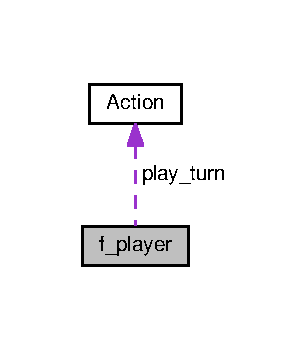
\includegraphics[width=148pt]{structf__player__coll__graph}
\end{center}
\end{figure}
\subsection*{Data Fields}
\begin{DoxyCompactItemize}
\item 
int($\ast$ \hyperlink{structf__player_ae803883f2825f7d13bbf12ad4c9b92ac}{init\-\_\-player} )(int id, int nb\-\_\-player, int nb\-\_\-towns, int nb\-\_\-rails, struct \hyperlink{structRail}{Rail} $\ast$rails, int nb\-\_\-wagons, int nb\-\_\-obj, struct \hyperlink{structObjective}{Objective} $\ast$objs)
\item 
struct \hyperlink{structAction}{Action}($\ast$ \hyperlink{structf__player_acbc97ea5cbb0c80c1a3ce98fea12c52e}{play\-\_\-turn} )(int $\ast$used\-\_\-wagons, int $\ast$cards\-\_\-in\-\_\-hand, int $\ast$objectives, int nb\-\_\-new\-\_\-rails, struct \hyperlink{structNew__rail}{New\-\_\-rail} $\ast$changes, int $\ast$new\-\_\-obj, int $\ast$cards)
\item 
int $\ast$($\ast$ \hyperlink{structf__player_a30b2a1a6dc61d60d60112b63199f72f6}{choose\-\_\-objective} )(int nb, int $\ast$objs, int min)
\item 
int($\ast$ \hyperlink{structf__player_ae47872a4531e4c79eb94348179812809}{free\-\_\-player} )()
\end{DoxyCompactItemize}


\subsection{Field Documentation}
\hypertarget{structf__player_a30b2a1a6dc61d60d60112b63199f72f6}{\index{f\-\_\-player@{f\-\_\-player}!choose\-\_\-objective@{choose\-\_\-objective}}
\index{choose\-\_\-objective@{choose\-\_\-objective}!f_player@{f\-\_\-player}}
\subsubsection[{choose\-\_\-objective}]{\setlength{\rightskip}{0pt plus 5cm}int$\ast$($\ast$ choose\-\_\-objective)(int nb, int $\ast$objs, int min)}}\label{structf__player_a30b2a1a6dc61d60d60112b63199f72f6}
\hypertarget{structf__player_ae47872a4531e4c79eb94348179812809}{\index{f\-\_\-player@{f\-\_\-player}!free\-\_\-player@{free\-\_\-player}}
\index{free\-\_\-player@{free\-\_\-player}!f_player@{f\-\_\-player}}
\subsubsection[{free\-\_\-player}]{\setlength{\rightskip}{0pt plus 5cm}int($\ast$ free\-\_\-player)()}}\label{structf__player_ae47872a4531e4c79eb94348179812809}
\hypertarget{structf__player_ae803883f2825f7d13bbf12ad4c9b92ac}{\index{f\-\_\-player@{f\-\_\-player}!init\-\_\-player@{init\-\_\-player}}
\index{init\-\_\-player@{init\-\_\-player}!f_player@{f\-\_\-player}}
\subsubsection[{init\-\_\-player}]{\setlength{\rightskip}{0pt plus 5cm}int($\ast$ init\-\_\-player)(int id, int nb\-\_\-player, int nb\-\_\-towns, int nb\-\_\-rails, struct {\bf Rail} $\ast$rails, int nb\-\_\-wagons, int nb\-\_\-obj, struct {\bf Objective} $\ast$objs)}}\label{structf__player_ae803883f2825f7d13bbf12ad4c9b92ac}
\hypertarget{structf__player_acbc97ea5cbb0c80c1a3ce98fea12c52e}{\index{f\-\_\-player@{f\-\_\-player}!play\-\_\-turn@{play\-\_\-turn}}
\index{play\-\_\-turn@{play\-\_\-turn}!f_player@{f\-\_\-player}}
\subsubsection[{play\-\_\-turn}]{\setlength{\rightskip}{0pt plus 5cm}struct {\bf Action}($\ast$ play\-\_\-turn)(int $\ast$used\-\_\-wagons, int $\ast$cards\-\_\-in\-\_\-hand, int $\ast$objectives, int nb\-\_\-new\-\_\-rails, struct {\bf New\-\_\-rail} $\ast$changes, int $\ast$new\-\_\-obj, int $\ast$cards)}}\label{structf__player_acbc97ea5cbb0c80c1a3ce98fea12c52e}


The documentation for this struct was generated from the following file\-:\begin{DoxyCompactItemize}
\item 
/net/malt/i/sbrouard/\-Documents/projets6/s6-\/rails-\/1992/trunk/src/\hyperlink{server_8h}{server.\-h}\end{DoxyCompactItemize}

\hypertarget{structLink}{\section{Link Struct Reference}
\label{structLink}\index{Link@{Link}}
}


The \hyperlink{structLink}{Link} struct is a structure composed of the number of ways (rails) between two given towns, and the tabular of the My\-\_\-rail(s) corresponding to those rails.  




{\ttfamily \#include $<$link.\-h$>$}



Collaboration diagram for Link\-:
\nopagebreak
\begin{figure}[H]
\begin{center}
\leavevmode
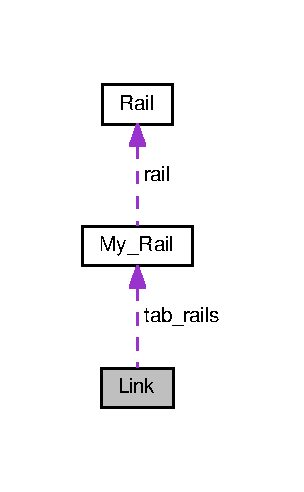
\includegraphics[width=146pt]{structLink__coll__graph}
\end{center}
\end{figure}
\subsection*{Data Fields}
\begin{DoxyCompactItemize}
\item 
int \hyperlink{structLink_a40cf4e4cf21e1686e79e3996ad0f6193}{nbr\-\_\-way}
\item 
struct \hyperlink{structMy__Rail}{My\-\_\-\-Rail} $\ast$ \hyperlink{structLink_ade94502d272c9618b413007c70ee7c83}{tab\-\_\-rails}
\end{DoxyCompactItemize}


\subsection{Detailed Description}
The \hyperlink{structLink}{Link} struct is a structure composed of the number of ways (rails) between two given towns, and the tabular of the My\-\_\-rail(s) corresponding to those rails. 

\subsection{Field Documentation}
\hypertarget{structLink_a40cf4e4cf21e1686e79e3996ad0f6193}{\index{Link@{Link}!nbr\-\_\-way@{nbr\-\_\-way}}
\index{nbr\-\_\-way@{nbr\-\_\-way}!Link@{Link}}
\subsubsection[{nbr\-\_\-way}]{\setlength{\rightskip}{0pt plus 5cm}int nbr\-\_\-way}}\label{structLink_a40cf4e4cf21e1686e79e3996ad0f6193}
\hypertarget{structLink_ade94502d272c9618b413007c70ee7c83}{\index{Link@{Link}!tab\-\_\-rails@{tab\-\_\-rails}}
\index{tab\-\_\-rails@{tab\-\_\-rails}!Link@{Link}}
\subsubsection[{tab\-\_\-rails}]{\setlength{\rightskip}{0pt plus 5cm}struct {\bf My\-\_\-\-Rail}$\ast$ tab\-\_\-rails}}\label{structLink_ade94502d272c9618b413007c70ee7c83}


The documentation for this struct was generated from the following file\-:\begin{DoxyCompactItemize}
\item 
/net/malt/i/sbrouard/\-Documents/projets6/s6-\/rails-\/1992/trunk/src/\hyperlink{link_8h}{link.\-h}\end{DoxyCompactItemize}

\hypertarget{structMap__info}{\section{Map\-\_\-info Struct Reference}
\label{structMap__info}\index{Map\-\_\-info@{Map\-\_\-info}}
}


{\ttfamily \#include $<$server.\-h$>$}

\subsection*{Data Fields}
\begin{DoxyCompactItemize}
\item 
int \hyperlink{structMap__info_ae5e7951963b1f7f7c7b80f42c7a6b04c}{nb\-\_\-towns}
\item 
int \hyperlink{structMap__info_a7c2cf198292c68f636c7c9be53dfbe82}{nb\-\_\-links}
\item 
int \hyperlink{structMap__info_af5511048dfe5f40291ef406c0c00bb1f}{nb\-\_\-objs}
\item 
int \hyperlink{structMap__info_a5fb8f492f437e97001f4f86eb758998b}{nb\-\_\-w\-\_\-player}
\end{DoxyCompactItemize}


\subsection{Field Documentation}
\hypertarget{structMap__info_a7c2cf198292c68f636c7c9be53dfbe82}{\index{Map\-\_\-info@{Map\-\_\-info}!nb\-\_\-links@{nb\-\_\-links}}
\index{nb\-\_\-links@{nb\-\_\-links}!Map_info@{Map\-\_\-info}}
\subsubsection[{nb\-\_\-links}]{\setlength{\rightskip}{0pt plus 5cm}int nb\-\_\-links}}\label{structMap__info_a7c2cf198292c68f636c7c9be53dfbe82}
\hypertarget{structMap__info_af5511048dfe5f40291ef406c0c00bb1f}{\index{Map\-\_\-info@{Map\-\_\-info}!nb\-\_\-objs@{nb\-\_\-objs}}
\index{nb\-\_\-objs@{nb\-\_\-objs}!Map_info@{Map\-\_\-info}}
\subsubsection[{nb\-\_\-objs}]{\setlength{\rightskip}{0pt plus 5cm}int nb\-\_\-objs}}\label{structMap__info_af5511048dfe5f40291ef406c0c00bb1f}
\hypertarget{structMap__info_ae5e7951963b1f7f7c7b80f42c7a6b04c}{\index{Map\-\_\-info@{Map\-\_\-info}!nb\-\_\-towns@{nb\-\_\-towns}}
\index{nb\-\_\-towns@{nb\-\_\-towns}!Map_info@{Map\-\_\-info}}
\subsubsection[{nb\-\_\-towns}]{\setlength{\rightskip}{0pt plus 5cm}int nb\-\_\-towns}}\label{structMap__info_ae5e7951963b1f7f7c7b80f42c7a6b04c}
\hypertarget{structMap__info_a5fb8f492f437e97001f4f86eb758998b}{\index{Map\-\_\-info@{Map\-\_\-info}!nb\-\_\-w\-\_\-player@{nb\-\_\-w\-\_\-player}}
\index{nb\-\_\-w\-\_\-player@{nb\-\_\-w\-\_\-player}!Map_info@{Map\-\_\-info}}
\subsubsection[{nb\-\_\-w\-\_\-player}]{\setlength{\rightskip}{0pt plus 5cm}int nb\-\_\-w\-\_\-player}}\label{structMap__info_a5fb8f492f437e97001f4f86eb758998b}


The documentation for this struct was generated from the following file\-:\begin{DoxyCompactItemize}
\item 
/net/malt/i/sbrouard/\-Documents/projets6/s6-\/rails-\/1992/trunk/src/\hyperlink{server_8h}{server.\-h}\end{DoxyCompactItemize}

\hypertarget{structMy__Rail}{\section{My\-\_\-\-Rail Struct Reference}
\label{structMy__Rail}\index{My\-\_\-\-Rail@{My\-\_\-\-Rail}}
}


The \hyperlink{structMy__Rail}{My\-\_\-\-Rail} struct is a structure composed of a pointer to a rail, the identifier of the player in the rail (-\/1 if none), and the identifier of the rail.  




{\ttfamily \#include $<$link.\-h$>$}



Collaboration diagram for My\-\_\-\-Rail\-:
\nopagebreak
\begin{figure}[H]
\begin{center}
\leavevmode
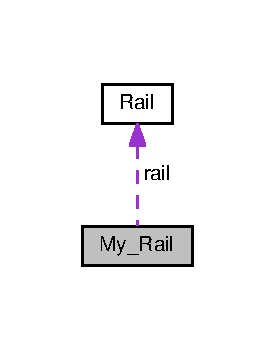
\includegraphics[width=132pt]{structMy__Rail__coll__graph}
\end{center}
\end{figure}
\subsection*{Data Fields}
\begin{DoxyCompactItemize}
\item 
struct \hyperlink{structRail}{Rail} const $\ast$ \hyperlink{structMy__Rail_ac3b4b1be4ff56fa71c889afa8c8c7888}{rail}
\item 
int \hyperlink{structMy__Rail_a7a793a40560fbe6a7df025a117e93272}{id\-\_\-player}
\item 
int \hyperlink{structMy__Rail_a79d06d37269735dfc8b180a8be0fe759}{id\-\_\-rail}
\end{DoxyCompactItemize}


\subsection{Detailed Description}
The \hyperlink{structMy__Rail}{My\-\_\-\-Rail} struct is a structure composed of a pointer to a rail, the identifier of the player in the rail (-\/1 if none), and the identifier of the rail. 

\subsection{Field Documentation}
\hypertarget{structMy__Rail_a7a793a40560fbe6a7df025a117e93272}{\index{My\-\_\-\-Rail@{My\-\_\-\-Rail}!id\-\_\-player@{id\-\_\-player}}
\index{id\-\_\-player@{id\-\_\-player}!My_Rail@{My\-\_\-\-Rail}}
\subsubsection[{id\-\_\-player}]{\setlength{\rightskip}{0pt plus 5cm}int id\-\_\-player}}\label{structMy__Rail_a7a793a40560fbe6a7df025a117e93272}
\hypertarget{structMy__Rail_a79d06d37269735dfc8b180a8be0fe759}{\index{My\-\_\-\-Rail@{My\-\_\-\-Rail}!id\-\_\-rail@{id\-\_\-rail}}
\index{id\-\_\-rail@{id\-\_\-rail}!My_Rail@{My\-\_\-\-Rail}}
\subsubsection[{id\-\_\-rail}]{\setlength{\rightskip}{0pt plus 5cm}int id\-\_\-rail}}\label{structMy__Rail_a79d06d37269735dfc8b180a8be0fe759}
\hypertarget{structMy__Rail_ac3b4b1be4ff56fa71c889afa8c8c7888}{\index{My\-\_\-\-Rail@{My\-\_\-\-Rail}!rail@{rail}}
\index{rail@{rail}!My_Rail@{My\-\_\-\-Rail}}
\subsubsection[{rail}]{\setlength{\rightskip}{0pt plus 5cm}struct {\bf Rail} const$\ast$ rail}}\label{structMy__Rail_ac3b4b1be4ff56fa71c889afa8c8c7888}


The documentation for this struct was generated from the following file\-:\begin{DoxyCompactItemize}
\item 
/net/malt/i/sbrouard/\-Documents/projets6/s6-\/rails-\/1992/trunk/src/\hyperlink{link_8h}{link.\-h}\end{DoxyCompactItemize}

\hypertarget{structNew__rail}{\section{New\-\_\-rail Struct Reference}
\label{structNew__rail}\index{New\-\_\-rail@{New\-\_\-rail}}
}


The \hyperlink{structNew__rail}{New\-\_\-rail} struct.  




{\ttfamily \#include $<$interface.\-h$>$}

\subsection*{Data Fields}
\begin{DoxyCompactItemize}
\item 
int \hyperlink{structNew__rail_a1017757e6fb62c1e1415b8663a5fc128}{rail}
\item 
int \hyperlink{structNew__rail_ae78f447e0fc84c538b91b0cc8c8a34fa}{player}
\end{DoxyCompactItemize}


\subsection{Detailed Description}
The \hyperlink{structNew__rail}{New\-\_\-rail} struct. 

\subsection{Field Documentation}
\hypertarget{structNew__rail_ae78f447e0fc84c538b91b0cc8c8a34fa}{\index{New\-\_\-rail@{New\-\_\-rail}!player@{player}}
\index{player@{player}!New_rail@{New\-\_\-rail}}
\subsubsection[{player}]{\setlength{\rightskip}{0pt plus 5cm}int player}}\label{structNew__rail_ae78f447e0fc84c538b91b0cc8c8a34fa}
\hypertarget{structNew__rail_a1017757e6fb62c1e1415b8663a5fc128}{\index{New\-\_\-rail@{New\-\_\-rail}!rail@{rail}}
\index{rail@{rail}!New_rail@{New\-\_\-rail}}
\subsubsection[{rail}]{\setlength{\rightskip}{0pt plus 5cm}int rail}}\label{structNew__rail_a1017757e6fb62c1e1415b8663a5fc128}


The documentation for this struct was generated from the following file\-:\begin{DoxyCompactItemize}
\item 
/net/malt/i/sbrouard/\-Documents/projets6/s6-\/rails-\/1992/trunk/src/\hyperlink{interface_8h}{interface.\-h}\end{DoxyCompactItemize}

\hypertarget{structObjective}{\section{Objective Struct Reference}
\label{structObjective}\index{Objective@{Objective}}
}


The \hyperlink{structObjective}{Objective} struct.  




{\ttfamily \#include $<$interface.\-h$>$}

\subsection*{Data Fields}
\begin{DoxyCompactItemize}
\item 
int \hyperlink{structObjective_a98fff246793d7da82f5befd043b04451}{town1}
\item 
int \hyperlink{structObjective_a38f94b482519ddfc27b054eb3dde308e}{town2}
\item 
int \hyperlink{structObjective_af7f8f4a4e39e09fdb5e9f02330ecabef}{points}
\end{DoxyCompactItemize}


\subsection{Detailed Description}
The \hyperlink{structObjective}{Objective} struct. 

\subsection{Field Documentation}
\hypertarget{structObjective_af7f8f4a4e39e09fdb5e9f02330ecabef}{\index{Objective@{Objective}!points@{points}}
\index{points@{points}!Objective@{Objective}}
\subsubsection[{points}]{\setlength{\rightskip}{0pt plus 5cm}int points}}\label{structObjective_af7f8f4a4e39e09fdb5e9f02330ecabef}
\hypertarget{structObjective_a98fff246793d7da82f5befd043b04451}{\index{Objective@{Objective}!town1@{town1}}
\index{town1@{town1}!Objective@{Objective}}
\subsubsection[{town1}]{\setlength{\rightskip}{0pt plus 5cm}int town1}}\label{structObjective_a98fff246793d7da82f5befd043b04451}
\hypertarget{structObjective_a38f94b482519ddfc27b054eb3dde308e}{\index{Objective@{Objective}!town2@{town2}}
\index{town2@{town2}!Objective@{Objective}}
\subsubsection[{town2}]{\setlength{\rightskip}{0pt plus 5cm}int town2}}\label{structObjective_a38f94b482519ddfc27b054eb3dde308e}


The documentation for this struct was generated from the following file\-:\begin{DoxyCompactItemize}
\item 
/net/malt/i/sbrouard/\-Documents/projets6/s6-\/rails-\/1992/trunk/src/\hyperlink{interface_8h}{interface.\-h}\end{DoxyCompactItemize}

\hypertarget{structPlayer}{\section{Player Struct Reference}
\label{structPlayer}\index{Player@{Player}}
}


{\ttfamily \#include $<$player.\-h$>$}



Collaboration diagram for Player\-:
\nopagebreak
\begin{figure}[H]
\begin{center}
\leavevmode
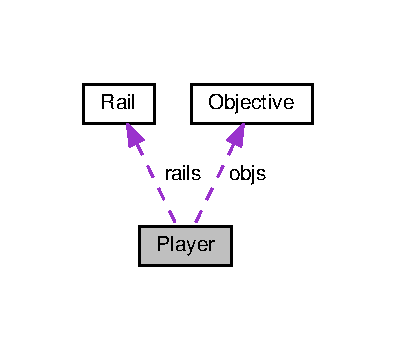
\includegraphics[width=190pt]{structPlayer__coll__graph}
\end{center}
\end{figure}
\subsection*{Data Fields}
\begin{DoxyCompactItemize}
\item 
int \hyperlink{structPlayer_a7a793a40560fbe6a7df025a117e93272}{id\-\_\-player}
\item 
int \hyperlink{structPlayer_af7f8f4a4e39e09fdb5e9f02330ecabef}{points}
\item 
int \hyperlink{structPlayer_a973dc11c7f9c09051fa782fde7863008}{nb\-\_\-players}
\item 
int \hyperlink{structPlayer_ae5e7951963b1f7f7c7b80f42c7a6b04c}{nb\-\_\-towns}
\item 
int \hyperlink{structPlayer_a124f37fc2c314fcfaf31544e4cd44e04}{nb\-\_\-colors}
\item 
int $\ast$ \hyperlink{structPlayer_a59bb1b4ae5e06f9146329fb82bfc1fd8}{nb\-\_\-remaining\-\_\-wagons}
\item 
int $\ast$ \hyperlink{structPlayer_a0fb92c4053d85148a96e9d22c796a76d}{nb\-\_\-remaining\-\_\-wagon\-\_\-cards}
\item 
int $\ast$ \hyperlink{structPlayer_a1773af477d4422d225e2611b07a0d562}{nb\-\_\-remaining\-\_\-objective\-\_\-cards}
\item 
int \hyperlink{structPlayer_a562c60af4150255b182aec231848d6ee}{nb\-\_\-rails}
\item 
struct \hyperlink{structRail}{Rail} $\ast$ \hyperlink{structPlayer_ac10a216b2c62ce10b7f08f2f9f4eb0b9}{rails}
\item 
int \hyperlink{structPlayer_acc2384127a7ee30a148aed382793ac45}{total\-\_\-nb\-\_\-obj}
\item 
struct \hyperlink{structObjective}{Objective} $\ast$ \hyperlink{structPlayer_a67d8ce3ce9168c68cd75c3055fd9ac38}{objs}
\item 
int \hyperlink{structPlayer_a433a97164a6a81495cbfa182ea9c1595}{nb\-\_\-personal\-\_\-objs}
\item 
int \hyperlink{structPlayer_ad3848dcc6461808764a8a9a2edd51f2e}{nb\-\_\-objs\-\_\-completed}
\item 
int $\ast$ \hyperlink{structPlayer_a8a02542940938a5fefa5bfe6dfeabb25}{personal\-\_\-objs}
\item 
int \hyperlink{structPlayer_a5bd2c82fb0dd0f0b540423e8793afe4d}{nb\-\_\-personal\-\_\-wagon\-\_\-cards}
\item 
int $\ast$ \hyperlink{structPlayer_a2fe65be556aa052d9443725c575df02e}{personal\-\_\-wagon\-\_\-cards}
\item 
int \hyperlink{structPlayer_a5b9e0fc618ea17cf04e114d28b2c253b}{nb\-\_\-objectives\-\_\-chosen}
\item 
int \hyperlink{structPlayer_a7c4c6059396a73859fc4dc4591f0c1af}{draw\-\_\-chosen}
\end{DoxyCompactItemize}


\subsection{Field Documentation}
\hypertarget{structPlayer_a7c4c6059396a73859fc4dc4591f0c1af}{\index{Player@{Player}!draw\-\_\-chosen@{draw\-\_\-chosen}}
\index{draw\-\_\-chosen@{draw\-\_\-chosen}!Player@{Player}}
\subsubsection[{draw\-\_\-chosen}]{\setlength{\rightskip}{0pt plus 5cm}int draw\-\_\-chosen}}\label{structPlayer_a7c4c6059396a73859fc4dc4591f0c1af}
\hypertarget{structPlayer_a7a793a40560fbe6a7df025a117e93272}{\index{Player@{Player}!id\-\_\-player@{id\-\_\-player}}
\index{id\-\_\-player@{id\-\_\-player}!Player@{Player}}
\subsubsection[{id\-\_\-player}]{\setlength{\rightskip}{0pt plus 5cm}int id\-\_\-player}}\label{structPlayer_a7a793a40560fbe6a7df025a117e93272}
\hypertarget{structPlayer_a124f37fc2c314fcfaf31544e4cd44e04}{\index{Player@{Player}!nb\-\_\-colors@{nb\-\_\-colors}}
\index{nb\-\_\-colors@{nb\-\_\-colors}!Player@{Player}}
\subsubsection[{nb\-\_\-colors}]{\setlength{\rightskip}{0pt plus 5cm}int nb\-\_\-colors}}\label{structPlayer_a124f37fc2c314fcfaf31544e4cd44e04}
\hypertarget{structPlayer_a5b9e0fc618ea17cf04e114d28b2c253b}{\index{Player@{Player}!nb\-\_\-objectives\-\_\-chosen@{nb\-\_\-objectives\-\_\-chosen}}
\index{nb\-\_\-objectives\-\_\-chosen@{nb\-\_\-objectives\-\_\-chosen}!Player@{Player}}
\subsubsection[{nb\-\_\-objectives\-\_\-chosen}]{\setlength{\rightskip}{0pt plus 5cm}int nb\-\_\-objectives\-\_\-chosen}}\label{structPlayer_a5b9e0fc618ea17cf04e114d28b2c253b}
\hypertarget{structPlayer_ad3848dcc6461808764a8a9a2edd51f2e}{\index{Player@{Player}!nb\-\_\-objs\-\_\-completed@{nb\-\_\-objs\-\_\-completed}}
\index{nb\-\_\-objs\-\_\-completed@{nb\-\_\-objs\-\_\-completed}!Player@{Player}}
\subsubsection[{nb\-\_\-objs\-\_\-completed}]{\setlength{\rightskip}{0pt plus 5cm}int nb\-\_\-objs\-\_\-completed}}\label{structPlayer_ad3848dcc6461808764a8a9a2edd51f2e}
\hypertarget{structPlayer_a433a97164a6a81495cbfa182ea9c1595}{\index{Player@{Player}!nb\-\_\-personal\-\_\-objs@{nb\-\_\-personal\-\_\-objs}}
\index{nb\-\_\-personal\-\_\-objs@{nb\-\_\-personal\-\_\-objs}!Player@{Player}}
\subsubsection[{nb\-\_\-personal\-\_\-objs}]{\setlength{\rightskip}{0pt plus 5cm}int nb\-\_\-personal\-\_\-objs}}\label{structPlayer_a433a97164a6a81495cbfa182ea9c1595}
\hypertarget{structPlayer_a5bd2c82fb0dd0f0b540423e8793afe4d}{\index{Player@{Player}!nb\-\_\-personal\-\_\-wagon\-\_\-cards@{nb\-\_\-personal\-\_\-wagon\-\_\-cards}}
\index{nb\-\_\-personal\-\_\-wagon\-\_\-cards@{nb\-\_\-personal\-\_\-wagon\-\_\-cards}!Player@{Player}}
\subsubsection[{nb\-\_\-personal\-\_\-wagon\-\_\-cards}]{\setlength{\rightskip}{0pt plus 5cm}int nb\-\_\-personal\-\_\-wagon\-\_\-cards}}\label{structPlayer_a5bd2c82fb0dd0f0b540423e8793afe4d}
\hypertarget{structPlayer_a973dc11c7f9c09051fa782fde7863008}{\index{Player@{Player}!nb\-\_\-players@{nb\-\_\-players}}
\index{nb\-\_\-players@{nb\-\_\-players}!Player@{Player}}
\subsubsection[{nb\-\_\-players}]{\setlength{\rightskip}{0pt plus 5cm}int nb\-\_\-players}}\label{structPlayer_a973dc11c7f9c09051fa782fde7863008}
\hypertarget{structPlayer_a562c60af4150255b182aec231848d6ee}{\index{Player@{Player}!nb\-\_\-rails@{nb\-\_\-rails}}
\index{nb\-\_\-rails@{nb\-\_\-rails}!Player@{Player}}
\subsubsection[{nb\-\_\-rails}]{\setlength{\rightskip}{0pt plus 5cm}int nb\-\_\-rails}}\label{structPlayer_a562c60af4150255b182aec231848d6ee}
\hypertarget{structPlayer_a1773af477d4422d225e2611b07a0d562}{\index{Player@{Player}!nb\-\_\-remaining\-\_\-objective\-\_\-cards@{nb\-\_\-remaining\-\_\-objective\-\_\-cards}}
\index{nb\-\_\-remaining\-\_\-objective\-\_\-cards@{nb\-\_\-remaining\-\_\-objective\-\_\-cards}!Player@{Player}}
\subsubsection[{nb\-\_\-remaining\-\_\-objective\-\_\-cards}]{\setlength{\rightskip}{0pt plus 5cm}int$\ast$ nb\-\_\-remaining\-\_\-objective\-\_\-cards}}\label{structPlayer_a1773af477d4422d225e2611b07a0d562}
\hypertarget{structPlayer_a0fb92c4053d85148a96e9d22c796a76d}{\index{Player@{Player}!nb\-\_\-remaining\-\_\-wagon\-\_\-cards@{nb\-\_\-remaining\-\_\-wagon\-\_\-cards}}
\index{nb\-\_\-remaining\-\_\-wagon\-\_\-cards@{nb\-\_\-remaining\-\_\-wagon\-\_\-cards}!Player@{Player}}
\subsubsection[{nb\-\_\-remaining\-\_\-wagon\-\_\-cards}]{\setlength{\rightskip}{0pt plus 5cm}int$\ast$ nb\-\_\-remaining\-\_\-wagon\-\_\-cards}}\label{structPlayer_a0fb92c4053d85148a96e9d22c796a76d}
\hypertarget{structPlayer_a59bb1b4ae5e06f9146329fb82bfc1fd8}{\index{Player@{Player}!nb\-\_\-remaining\-\_\-wagons@{nb\-\_\-remaining\-\_\-wagons}}
\index{nb\-\_\-remaining\-\_\-wagons@{nb\-\_\-remaining\-\_\-wagons}!Player@{Player}}
\subsubsection[{nb\-\_\-remaining\-\_\-wagons}]{\setlength{\rightskip}{0pt plus 5cm}int$\ast$ nb\-\_\-remaining\-\_\-wagons}}\label{structPlayer_a59bb1b4ae5e06f9146329fb82bfc1fd8}
\hypertarget{structPlayer_ae5e7951963b1f7f7c7b80f42c7a6b04c}{\index{Player@{Player}!nb\-\_\-towns@{nb\-\_\-towns}}
\index{nb\-\_\-towns@{nb\-\_\-towns}!Player@{Player}}
\subsubsection[{nb\-\_\-towns}]{\setlength{\rightskip}{0pt plus 5cm}int nb\-\_\-towns}}\label{structPlayer_ae5e7951963b1f7f7c7b80f42c7a6b04c}
\hypertarget{structPlayer_a67d8ce3ce9168c68cd75c3055fd9ac38}{\index{Player@{Player}!objs@{objs}}
\index{objs@{objs}!Player@{Player}}
\subsubsection[{objs}]{\setlength{\rightskip}{0pt plus 5cm}struct {\bf Objective}$\ast$ objs}}\label{structPlayer_a67d8ce3ce9168c68cd75c3055fd9ac38}
\hypertarget{structPlayer_a8a02542940938a5fefa5bfe6dfeabb25}{\index{Player@{Player}!personal\-\_\-objs@{personal\-\_\-objs}}
\index{personal\-\_\-objs@{personal\-\_\-objs}!Player@{Player}}
\subsubsection[{personal\-\_\-objs}]{\setlength{\rightskip}{0pt plus 5cm}int$\ast$ personal\-\_\-objs}}\label{structPlayer_a8a02542940938a5fefa5bfe6dfeabb25}
\hypertarget{structPlayer_a2fe65be556aa052d9443725c575df02e}{\index{Player@{Player}!personal\-\_\-wagon\-\_\-cards@{personal\-\_\-wagon\-\_\-cards}}
\index{personal\-\_\-wagon\-\_\-cards@{personal\-\_\-wagon\-\_\-cards}!Player@{Player}}
\subsubsection[{personal\-\_\-wagon\-\_\-cards}]{\setlength{\rightskip}{0pt plus 5cm}int$\ast$ personal\-\_\-wagon\-\_\-cards}}\label{structPlayer_a2fe65be556aa052d9443725c575df02e}
\hypertarget{structPlayer_af7f8f4a4e39e09fdb5e9f02330ecabef}{\index{Player@{Player}!points@{points}}
\index{points@{points}!Player@{Player}}
\subsubsection[{points}]{\setlength{\rightskip}{0pt plus 5cm}int points}}\label{structPlayer_af7f8f4a4e39e09fdb5e9f02330ecabef}
\hypertarget{structPlayer_ac10a216b2c62ce10b7f08f2f9f4eb0b9}{\index{Player@{Player}!rails@{rails}}
\index{rails@{rails}!Player@{Player}}
\subsubsection[{rails}]{\setlength{\rightskip}{0pt plus 5cm}struct {\bf Rail}$\ast$ rails}}\label{structPlayer_ac10a216b2c62ce10b7f08f2f9f4eb0b9}
\hypertarget{structPlayer_acc2384127a7ee30a148aed382793ac45}{\index{Player@{Player}!total\-\_\-nb\-\_\-obj@{total\-\_\-nb\-\_\-obj}}
\index{total\-\_\-nb\-\_\-obj@{total\-\_\-nb\-\_\-obj}!Player@{Player}}
\subsubsection[{total\-\_\-nb\-\_\-obj}]{\setlength{\rightskip}{0pt plus 5cm}int total\-\_\-nb\-\_\-obj}}\label{structPlayer_acc2384127a7ee30a148aed382793ac45}


The documentation for this struct was generated from the following file\-:\begin{DoxyCompactItemize}
\item 
/net/malt/i/sbrouard/\-Documents/projets6/s6-\/rails-\/1992/trunk/src/\hyperlink{player_8h}{player.\-h}\end{DoxyCompactItemize}

\hypertarget{structRail}{\section{Rail Struct Reference}
\label{structRail}\index{Rail@{Rail}}
}


The \hyperlink{structRail}{Rail} struct.  




{\ttfamily \#include $<$interface.\-h$>$}

\subsection*{Data Fields}
\begin{DoxyCompactItemize}
\item 
int \hyperlink{structRail_a98fff246793d7da82f5befd043b04451}{town1}
\item 
int \hyperlink{structRail_a38f94b482519ddfc27b054eb3dde308e}{town2}
\item 
int \hyperlink{structRail_a9f59b34b1f25fe00023291b678246bcc}{length}
\item 
int \hyperlink{structRail_a0fd02fb9277ffcb35a75066ffe95e8c7}{color}
\end{DoxyCompactItemize}


\subsection{Detailed Description}
The \hyperlink{structRail}{Rail} struct. 

\subsection{Field Documentation}
\hypertarget{structRail_a0fd02fb9277ffcb35a75066ffe95e8c7}{\index{Rail@{Rail}!color@{color}}
\index{color@{color}!Rail@{Rail}}
\subsubsection[{color}]{\setlength{\rightskip}{0pt plus 5cm}int color}}\label{structRail_a0fd02fb9277ffcb35a75066ffe95e8c7}
\hypertarget{structRail_a9f59b34b1f25fe00023291b678246bcc}{\index{Rail@{Rail}!length@{length}}
\index{length@{length}!Rail@{Rail}}
\subsubsection[{length}]{\setlength{\rightskip}{0pt plus 5cm}int length}}\label{structRail_a9f59b34b1f25fe00023291b678246bcc}
\hypertarget{structRail_a98fff246793d7da82f5befd043b04451}{\index{Rail@{Rail}!town1@{town1}}
\index{town1@{town1}!Rail@{Rail}}
\subsubsection[{town1}]{\setlength{\rightskip}{0pt plus 5cm}int town1}}\label{structRail_a98fff246793d7da82f5befd043b04451}
\hypertarget{structRail_a38f94b482519ddfc27b054eb3dde308e}{\index{Rail@{Rail}!town2@{town2}}
\index{town2@{town2}!Rail@{Rail}}
\subsubsection[{town2}]{\setlength{\rightskip}{0pt plus 5cm}int town2}}\label{structRail_a38f94b482519ddfc27b054eb3dde308e}


The documentation for this struct was generated from the following file\-:\begin{DoxyCompactItemize}
\item 
/net/malt/i/sbrouard/\-Documents/projets6/s6-\/rails-\/1992/trunk/src/\hyperlink{interface_8h}{interface.\-h}\end{DoxyCompactItemize}

\chapter{File Documentation}
\hypertarget{CMakeCCompilerId_8c}{\section{/net/malt/i/sbrouard/\-Documents/projets6/s6-\/rails-\/1992/trunk/build/\-C\-Make\-Files/2.8.12.2/\-Compiler\-Id\-C/\-C\-Make\-C\-Compiler\-Id.c File Reference}
\label{CMakeCCompilerId_8c}\index{/net/malt/i/sbrouard/\-Documents/projets6/s6-\/rails-\/1992/trunk/build/\-C\-Make\-Files/2.\-8.\-12.\-2/\-Compiler\-Id\-C/\-C\-Make\-C\-Compiler\-Id.\-c@{/net/malt/i/sbrouard/\-Documents/projets6/s6-\/rails-\/1992/trunk/build/\-C\-Make\-Files/2.\-8.\-12.\-2/\-Compiler\-Id\-C/\-C\-Make\-C\-Compiler\-Id.\-c}}
}
\subsection*{Macros}
\begin{DoxyCompactItemize}
\item 
\#define \hyperlink{CMakeCCompilerId_8c_a81dee0709ded976b2e0319239f72d174}{C\-O\-M\-P\-I\-L\-E\-R\-\_\-\-I\-D}~\char`\"{}\char`\"{}
\item 
\#define \hyperlink{CMakeCCompilerId_8c_adbc5372f40838899018fadbc89bd588b}{P\-L\-A\-T\-F\-O\-R\-M\-\_\-\-I\-D}~\char`\"{}\char`\"{}
\item 
\#define \hyperlink{CMakeCCompilerId_8c_aba35d0d200deaeb06aee95ca297acb28}{A\-R\-C\-H\-I\-T\-E\-C\-T\-U\-R\-E\-\_\-\-I\-D}~\char`\"{}\char`\"{}
\item 
\#define \hyperlink{CMakeCCompilerId_8c_ad1280362da42492bbc11aa78cbf776ad}{D\-E\-C}(n)
\item 
\#define \hyperlink{CMakeCCompilerId_8c_a46d5d95daa1bef867bd0179594310ed5}{H\-E\-X}(n)
\end{DoxyCompactItemize}
\subsection*{Functions}
\begin{DoxyCompactItemize}
\item 
int \hyperlink{CMakeCCompilerId_8c_a0ddf1224851353fc92bfbff6f499fa97}{main} (int argc, char $\ast$argv\mbox{[}$\,$\mbox{]})
\end{DoxyCompactItemize}
\subsection*{Variables}
\begin{DoxyCompactItemize}
\item 
char const $\ast$ \hyperlink{CMakeCCompilerId_8c_a4b0efeb7a5d59313986b3a0390f050f6}{info\-\_\-compiler} = \char`\"{}I\-N\-F\-O\char`\"{} \char`\"{}\-:\char`\"{} \char`\"{}compiler\mbox{[}\char`\"{} C\-O\-M\-P\-I\-L\-E\-R\-\_\-\-I\-D \char`\"{}\mbox{]}\char`\"{}
\item 
char const $\ast$ \hyperlink{CMakeCCompilerId_8c_a2321403dee54ee23f0c2fa849c60f7d4}{info\-\_\-platform} = \char`\"{}I\-N\-F\-O\char`\"{} \char`\"{}\-:\char`\"{} \char`\"{}platform\mbox{[}\char`\"{} P\-L\-A\-T\-F\-O\-R\-M\-\_\-\-I\-D \char`\"{}\mbox{]}\char`\"{}
\item 
char const $\ast$ \hyperlink{CMakeCCompilerId_8c_a59647e99d304ed33b15cb284c27ed391}{info\-\_\-arch} = \char`\"{}I\-N\-F\-O\char`\"{} \char`\"{}\-:\char`\"{} \char`\"{}arch\mbox{[}\char`\"{} A\-R\-C\-H\-I\-T\-E\-C\-T\-U\-R\-E\-\_\-\-I\-D \char`\"{}\mbox{]}\char`\"{}
\end{DoxyCompactItemize}


\subsection{Macro Definition Documentation}
\hypertarget{CMakeCCompilerId_8c_aba35d0d200deaeb06aee95ca297acb28}{\index{C\-Make\-C\-Compiler\-Id.\-c@{C\-Make\-C\-Compiler\-Id.\-c}!A\-R\-C\-H\-I\-T\-E\-C\-T\-U\-R\-E\-\_\-\-I\-D@{A\-R\-C\-H\-I\-T\-E\-C\-T\-U\-R\-E\-\_\-\-I\-D}}
\index{A\-R\-C\-H\-I\-T\-E\-C\-T\-U\-R\-E\-\_\-\-I\-D@{A\-R\-C\-H\-I\-T\-E\-C\-T\-U\-R\-E\-\_\-\-I\-D}!CMakeCCompilerId.c@{C\-Make\-C\-Compiler\-Id.\-c}}
\subsubsection[{A\-R\-C\-H\-I\-T\-E\-C\-T\-U\-R\-E\-\_\-\-I\-D}]{\setlength{\rightskip}{0pt plus 5cm}\#define A\-R\-C\-H\-I\-T\-E\-C\-T\-U\-R\-E\-\_\-\-I\-D~\char`\"{}\char`\"{}}}\label{CMakeCCompilerId_8c_aba35d0d200deaeb06aee95ca297acb28}
\hypertarget{CMakeCCompilerId_8c_a81dee0709ded976b2e0319239f72d174}{\index{C\-Make\-C\-Compiler\-Id.\-c@{C\-Make\-C\-Compiler\-Id.\-c}!C\-O\-M\-P\-I\-L\-E\-R\-\_\-\-I\-D@{C\-O\-M\-P\-I\-L\-E\-R\-\_\-\-I\-D}}
\index{C\-O\-M\-P\-I\-L\-E\-R\-\_\-\-I\-D@{C\-O\-M\-P\-I\-L\-E\-R\-\_\-\-I\-D}!CMakeCCompilerId.c@{C\-Make\-C\-Compiler\-Id.\-c}}
\subsubsection[{C\-O\-M\-P\-I\-L\-E\-R\-\_\-\-I\-D}]{\setlength{\rightskip}{0pt plus 5cm}\#define C\-O\-M\-P\-I\-L\-E\-R\-\_\-\-I\-D~\char`\"{}\char`\"{}}}\label{CMakeCCompilerId_8c_a81dee0709ded976b2e0319239f72d174}
\hypertarget{CMakeCCompilerId_8c_ad1280362da42492bbc11aa78cbf776ad}{\index{C\-Make\-C\-Compiler\-Id.\-c@{C\-Make\-C\-Compiler\-Id.\-c}!D\-E\-C@{D\-E\-C}}
\index{D\-E\-C@{D\-E\-C}!CMakeCCompilerId.c@{C\-Make\-C\-Compiler\-Id.\-c}}
\subsubsection[{D\-E\-C}]{\setlength{\rightskip}{0pt plus 5cm}\#define D\-E\-C(
\begin{DoxyParamCaption}
\item[{}]{n}
\end{DoxyParamCaption}
)}}\label{CMakeCCompilerId_8c_ad1280362da42492bbc11aa78cbf776ad}
{\bfseries Value\-:}
\begin{DoxyCode}
(\textcolor{charliteral}{'0'} + (((n) / 10000000)%10)), \(\backslash\)
  (\textcolor{charliteral}{'0'} + (((n) / 1000000)%10)),  \(\backslash\)
  (\textcolor{charliteral}{'0'} + (((n) / 100000)%10)),   \(\backslash\)
  (\textcolor{charliteral}{'0'} + (((n) / 10000)%10)),    \(\backslash\)
  (\textcolor{charliteral}{'0'} + (((n) / 1000)%10)),     \(\backslash\)
  (\textcolor{charliteral}{'0'} + (((n) / 100)%10)),      \(\backslash\)
  (\textcolor{charliteral}{'0'} + (((n) / 10)%10)),       \(\backslash\)
  (\textcolor{charliteral}{'0'} +  ((n) % 10))
\end{DoxyCode}
\hypertarget{CMakeCCompilerId_8c_a46d5d95daa1bef867bd0179594310ed5}{\index{C\-Make\-C\-Compiler\-Id.\-c@{C\-Make\-C\-Compiler\-Id.\-c}!H\-E\-X@{H\-E\-X}}
\index{H\-E\-X@{H\-E\-X}!CMakeCCompilerId.c@{C\-Make\-C\-Compiler\-Id.\-c}}
\subsubsection[{H\-E\-X}]{\setlength{\rightskip}{0pt plus 5cm}\#define H\-E\-X(
\begin{DoxyParamCaption}
\item[{}]{n}
\end{DoxyParamCaption}
)}}\label{CMakeCCompilerId_8c_a46d5d95daa1bef867bd0179594310ed5}
{\bfseries Value\-:}
\begin{DoxyCode}
(\textcolor{charliteral}{'0'} + ((n)>>28 & 0xF)), \(\backslash\)
  (\textcolor{charliteral}{'0'} + ((n)>>24 & 0xF)), \(\backslash\)
  (\textcolor{charliteral}{'0'} + ((n)>>20 & 0xF)), \(\backslash\)
  (\textcolor{charliteral}{'0'} + ((n)>>16 & 0xF)), \(\backslash\)
  (\textcolor{charliteral}{'0'} + ((n)>>12 & 0xF)), \(\backslash\)
  (\textcolor{charliteral}{'0'} + ((n)>>8  & 0xF)), \(\backslash\)
  (\textcolor{charliteral}{'0'} + ((n)>>4  & 0xF)), \(\backslash\)
  (\textcolor{charliteral}{'0'} + ((n)     & 0xF))
\end{DoxyCode}
\hypertarget{CMakeCCompilerId_8c_adbc5372f40838899018fadbc89bd588b}{\index{C\-Make\-C\-Compiler\-Id.\-c@{C\-Make\-C\-Compiler\-Id.\-c}!P\-L\-A\-T\-F\-O\-R\-M\-\_\-\-I\-D@{P\-L\-A\-T\-F\-O\-R\-M\-\_\-\-I\-D}}
\index{P\-L\-A\-T\-F\-O\-R\-M\-\_\-\-I\-D@{P\-L\-A\-T\-F\-O\-R\-M\-\_\-\-I\-D}!CMakeCCompilerId.c@{C\-Make\-C\-Compiler\-Id.\-c}}
\subsubsection[{P\-L\-A\-T\-F\-O\-R\-M\-\_\-\-I\-D}]{\setlength{\rightskip}{0pt plus 5cm}\#define P\-L\-A\-T\-F\-O\-R\-M\-\_\-\-I\-D~\char`\"{}\char`\"{}}}\label{CMakeCCompilerId_8c_adbc5372f40838899018fadbc89bd588b}


\subsection{Function Documentation}
\hypertarget{CMakeCCompilerId_8c_a0ddf1224851353fc92bfbff6f499fa97}{\index{C\-Make\-C\-Compiler\-Id.\-c@{C\-Make\-C\-Compiler\-Id.\-c}!main@{main}}
\index{main@{main}!CMakeCCompilerId.c@{C\-Make\-C\-Compiler\-Id.\-c}}
\subsubsection[{main}]{\setlength{\rightskip}{0pt plus 5cm}int main (
\begin{DoxyParamCaption}
\item[{int}]{argc, }
\item[{char $\ast$}]{argv\mbox{[}$\,$\mbox{]}}
\end{DoxyParamCaption}
)}}\label{CMakeCCompilerId_8c_a0ddf1224851353fc92bfbff6f499fa97}


\subsection{Variable Documentation}
\hypertarget{CMakeCCompilerId_8c_a59647e99d304ed33b15cb284c27ed391}{\index{C\-Make\-C\-Compiler\-Id.\-c@{C\-Make\-C\-Compiler\-Id.\-c}!info\-\_\-arch@{info\-\_\-arch}}
\index{info\-\_\-arch@{info\-\_\-arch}!CMakeCCompilerId.c@{C\-Make\-C\-Compiler\-Id.\-c}}
\subsubsection[{info\-\_\-arch}]{\setlength{\rightskip}{0pt plus 5cm}char const$\ast$ info\-\_\-arch = \char`\"{}I\-N\-F\-O\char`\"{} \char`\"{}\-:\char`\"{} \char`\"{}arch\mbox{[}\char`\"{} A\-R\-C\-H\-I\-T\-E\-C\-T\-U\-R\-E\-\_\-\-I\-D \char`\"{}\mbox{]}\char`\"{}}}\label{CMakeCCompilerId_8c_a59647e99d304ed33b15cb284c27ed391}
\hypertarget{CMakeCCompilerId_8c_a4b0efeb7a5d59313986b3a0390f050f6}{\index{C\-Make\-C\-Compiler\-Id.\-c@{C\-Make\-C\-Compiler\-Id.\-c}!info\-\_\-compiler@{info\-\_\-compiler}}
\index{info\-\_\-compiler@{info\-\_\-compiler}!CMakeCCompilerId.c@{C\-Make\-C\-Compiler\-Id.\-c}}
\subsubsection[{info\-\_\-compiler}]{\setlength{\rightskip}{0pt plus 5cm}char const$\ast$ info\-\_\-compiler = \char`\"{}I\-N\-F\-O\char`\"{} \char`\"{}\-:\char`\"{} \char`\"{}compiler\mbox{[}\char`\"{} C\-O\-M\-P\-I\-L\-E\-R\-\_\-\-I\-D \char`\"{}\mbox{]}\char`\"{}}}\label{CMakeCCompilerId_8c_a4b0efeb7a5d59313986b3a0390f050f6}
\hypertarget{CMakeCCompilerId_8c_a2321403dee54ee23f0c2fa849c60f7d4}{\index{C\-Make\-C\-Compiler\-Id.\-c@{C\-Make\-C\-Compiler\-Id.\-c}!info\-\_\-platform@{info\-\_\-platform}}
\index{info\-\_\-platform@{info\-\_\-platform}!CMakeCCompilerId.c@{C\-Make\-C\-Compiler\-Id.\-c}}
\subsubsection[{info\-\_\-platform}]{\setlength{\rightskip}{0pt plus 5cm}char const$\ast$ info\-\_\-platform = \char`\"{}I\-N\-F\-O\char`\"{} \char`\"{}\-:\char`\"{} \char`\"{}platform\mbox{[}\char`\"{} P\-L\-A\-T\-F\-O\-R\-M\-\_\-\-I\-D \char`\"{}\mbox{]}\char`\"{}}}\label{CMakeCCompilerId_8c_a2321403dee54ee23f0c2fa849c60f7d4}

\hypertarget{CMakeCXXCompilerId_8cpp}{\section{/net/malt/i/sbrouard/\-Documents/projets6/s6-\/rails-\/1992/trunk/build/\-C\-Make\-Files/2.8.12.2/\-Compiler\-Id\-C\-X\-X/\-C\-Make\-C\-X\-X\-Compiler\-Id.cpp File Reference}
\label{CMakeCXXCompilerId_8cpp}\index{/net/malt/i/sbrouard/\-Documents/projets6/s6-\/rails-\/1992/trunk/build/\-C\-Make\-Files/2.\-8.\-12.\-2/\-Compiler\-Id\-C\-X\-X/\-C\-Make\-C\-X\-X\-Compiler\-Id.\-cpp@{/net/malt/i/sbrouard/\-Documents/projets6/s6-\/rails-\/1992/trunk/build/\-C\-Make\-Files/2.\-8.\-12.\-2/\-Compiler\-Id\-C\-X\-X/\-C\-Make\-C\-X\-X\-Compiler\-Id.\-cpp}}
}
\subsection*{Macros}
\begin{DoxyCompactItemize}
\item 
\#define \hyperlink{CMakeCXXCompilerId_8cpp_a81dee0709ded976b2e0319239f72d174}{C\-O\-M\-P\-I\-L\-E\-R\-\_\-\-I\-D}~\char`\"{}\char`\"{}
\item 
\#define \hyperlink{CMakeCXXCompilerId_8cpp_adbc5372f40838899018fadbc89bd588b}{P\-L\-A\-T\-F\-O\-R\-M\-\_\-\-I\-D}~\char`\"{}\char`\"{}
\item 
\#define \hyperlink{CMakeCXXCompilerId_8cpp_aba35d0d200deaeb06aee95ca297acb28}{A\-R\-C\-H\-I\-T\-E\-C\-T\-U\-R\-E\-\_\-\-I\-D}~\char`\"{}\char`\"{}
\item 
\#define \hyperlink{CMakeCXXCompilerId_8cpp_ad1280362da42492bbc11aa78cbf776ad}{D\-E\-C}(n)
\item 
\#define \hyperlink{CMakeCXXCompilerId_8cpp_a46d5d95daa1bef867bd0179594310ed5}{H\-E\-X}(n)
\end{DoxyCompactItemize}
\subsection*{Functions}
\begin{DoxyCompactItemize}
\item 
int \hyperlink{CMakeCXXCompilerId_8cpp_a0ddf1224851353fc92bfbff6f499fa97}{main} (int argc, char $\ast$argv\mbox{[}$\,$\mbox{]})
\end{DoxyCompactItemize}
\subsection*{Variables}
\begin{DoxyCompactItemize}
\item 
char const $\ast$ \hyperlink{CMakeCXXCompilerId_8cpp_a4b0efeb7a5d59313986b3a0390f050f6}{info\-\_\-compiler} = \char`\"{}I\-N\-F\-O\char`\"{} \char`\"{}\-:\char`\"{} \char`\"{}compiler\mbox{[}\char`\"{} C\-O\-M\-P\-I\-L\-E\-R\-\_\-\-I\-D \char`\"{}\mbox{]}\char`\"{}
\item 
char const $\ast$ \hyperlink{CMakeCXXCompilerId_8cpp_a2321403dee54ee23f0c2fa849c60f7d4}{info\-\_\-platform} = \char`\"{}I\-N\-F\-O\char`\"{} \char`\"{}\-:\char`\"{} \char`\"{}platform\mbox{[}\char`\"{} P\-L\-A\-T\-F\-O\-R\-M\-\_\-\-I\-D \char`\"{}\mbox{]}\char`\"{}
\item 
char const $\ast$ \hyperlink{CMakeCXXCompilerId_8cpp_a59647e99d304ed33b15cb284c27ed391}{info\-\_\-arch} = \char`\"{}I\-N\-F\-O\char`\"{} \char`\"{}\-:\char`\"{} \char`\"{}arch\mbox{[}\char`\"{} A\-R\-C\-H\-I\-T\-E\-C\-T\-U\-R\-E\-\_\-\-I\-D \char`\"{}\mbox{]}\char`\"{}
\end{DoxyCompactItemize}


\subsection{Macro Definition Documentation}
\hypertarget{CMakeCXXCompilerId_8cpp_aba35d0d200deaeb06aee95ca297acb28}{\index{C\-Make\-C\-X\-X\-Compiler\-Id.\-cpp@{C\-Make\-C\-X\-X\-Compiler\-Id.\-cpp}!A\-R\-C\-H\-I\-T\-E\-C\-T\-U\-R\-E\-\_\-\-I\-D@{A\-R\-C\-H\-I\-T\-E\-C\-T\-U\-R\-E\-\_\-\-I\-D}}
\index{A\-R\-C\-H\-I\-T\-E\-C\-T\-U\-R\-E\-\_\-\-I\-D@{A\-R\-C\-H\-I\-T\-E\-C\-T\-U\-R\-E\-\_\-\-I\-D}!CMakeCXXCompilerId.cpp@{C\-Make\-C\-X\-X\-Compiler\-Id.\-cpp}}
\subsubsection[{A\-R\-C\-H\-I\-T\-E\-C\-T\-U\-R\-E\-\_\-\-I\-D}]{\setlength{\rightskip}{0pt plus 5cm}\#define A\-R\-C\-H\-I\-T\-E\-C\-T\-U\-R\-E\-\_\-\-I\-D~\char`\"{}\char`\"{}}}\label{CMakeCXXCompilerId_8cpp_aba35d0d200deaeb06aee95ca297acb28}
\hypertarget{CMakeCXXCompilerId_8cpp_a81dee0709ded976b2e0319239f72d174}{\index{C\-Make\-C\-X\-X\-Compiler\-Id.\-cpp@{C\-Make\-C\-X\-X\-Compiler\-Id.\-cpp}!C\-O\-M\-P\-I\-L\-E\-R\-\_\-\-I\-D@{C\-O\-M\-P\-I\-L\-E\-R\-\_\-\-I\-D}}
\index{C\-O\-M\-P\-I\-L\-E\-R\-\_\-\-I\-D@{C\-O\-M\-P\-I\-L\-E\-R\-\_\-\-I\-D}!CMakeCXXCompilerId.cpp@{C\-Make\-C\-X\-X\-Compiler\-Id.\-cpp}}
\subsubsection[{C\-O\-M\-P\-I\-L\-E\-R\-\_\-\-I\-D}]{\setlength{\rightskip}{0pt plus 5cm}\#define C\-O\-M\-P\-I\-L\-E\-R\-\_\-\-I\-D~\char`\"{}\char`\"{}}}\label{CMakeCXXCompilerId_8cpp_a81dee0709ded976b2e0319239f72d174}
\hypertarget{CMakeCXXCompilerId_8cpp_ad1280362da42492bbc11aa78cbf776ad}{\index{C\-Make\-C\-X\-X\-Compiler\-Id.\-cpp@{C\-Make\-C\-X\-X\-Compiler\-Id.\-cpp}!D\-E\-C@{D\-E\-C}}
\index{D\-E\-C@{D\-E\-C}!CMakeCXXCompilerId.cpp@{C\-Make\-C\-X\-X\-Compiler\-Id.\-cpp}}
\subsubsection[{D\-E\-C}]{\setlength{\rightskip}{0pt plus 5cm}\#define D\-E\-C(
\begin{DoxyParamCaption}
\item[{}]{n}
\end{DoxyParamCaption}
)}}\label{CMakeCXXCompilerId_8cpp_ad1280362da42492bbc11aa78cbf776ad}
{\bfseries Value\-:}
\begin{DoxyCode}
(\textcolor{charliteral}{'0'} + (((n) / 10000000)%10)), \(\backslash\)
  (\textcolor{charliteral}{'0'} + (((n) / 1000000)%10)),  \(\backslash\)
  (\textcolor{charliteral}{'0'} + (((n) / 100000)%10)),   \(\backslash\)
  (\textcolor{charliteral}{'0'} + (((n) / 10000)%10)),    \(\backslash\)
  (\textcolor{charliteral}{'0'} + (((n) / 1000)%10)),     \(\backslash\)
  (\textcolor{charliteral}{'0'} + (((n) / 100)%10)),      \(\backslash\)
  (\textcolor{charliteral}{'0'} + (((n) / 10)%10)),       \(\backslash\)
  (\textcolor{charliteral}{'0'} +  ((n) % 10))
\end{DoxyCode}
\hypertarget{CMakeCXXCompilerId_8cpp_a46d5d95daa1bef867bd0179594310ed5}{\index{C\-Make\-C\-X\-X\-Compiler\-Id.\-cpp@{C\-Make\-C\-X\-X\-Compiler\-Id.\-cpp}!H\-E\-X@{H\-E\-X}}
\index{H\-E\-X@{H\-E\-X}!CMakeCXXCompilerId.cpp@{C\-Make\-C\-X\-X\-Compiler\-Id.\-cpp}}
\subsubsection[{H\-E\-X}]{\setlength{\rightskip}{0pt plus 5cm}\#define H\-E\-X(
\begin{DoxyParamCaption}
\item[{}]{n}
\end{DoxyParamCaption}
)}}\label{CMakeCXXCompilerId_8cpp_a46d5d95daa1bef867bd0179594310ed5}
{\bfseries Value\-:}
\begin{DoxyCode}
(\textcolor{charliteral}{'0'} + ((n)>>28 & 0xF)), \(\backslash\)
  (\textcolor{charliteral}{'0'} + ((n)>>24 & 0xF)), \(\backslash\)
  (\textcolor{charliteral}{'0'} + ((n)>>20 & 0xF)), \(\backslash\)
  (\textcolor{charliteral}{'0'} + ((n)>>16 & 0xF)), \(\backslash\)
  (\textcolor{charliteral}{'0'} + ((n)>>12 & 0xF)), \(\backslash\)
  (\textcolor{charliteral}{'0'} + ((n)>>8  & 0xF)), \(\backslash\)
  (\textcolor{charliteral}{'0'} + ((n)>>4  & 0xF)), \(\backslash\)
  (\textcolor{charliteral}{'0'} + ((n)     & 0xF))
\end{DoxyCode}
\hypertarget{CMakeCXXCompilerId_8cpp_adbc5372f40838899018fadbc89bd588b}{\index{C\-Make\-C\-X\-X\-Compiler\-Id.\-cpp@{C\-Make\-C\-X\-X\-Compiler\-Id.\-cpp}!P\-L\-A\-T\-F\-O\-R\-M\-\_\-\-I\-D@{P\-L\-A\-T\-F\-O\-R\-M\-\_\-\-I\-D}}
\index{P\-L\-A\-T\-F\-O\-R\-M\-\_\-\-I\-D@{P\-L\-A\-T\-F\-O\-R\-M\-\_\-\-I\-D}!CMakeCXXCompilerId.cpp@{C\-Make\-C\-X\-X\-Compiler\-Id.\-cpp}}
\subsubsection[{P\-L\-A\-T\-F\-O\-R\-M\-\_\-\-I\-D}]{\setlength{\rightskip}{0pt plus 5cm}\#define P\-L\-A\-T\-F\-O\-R\-M\-\_\-\-I\-D~\char`\"{}\char`\"{}}}\label{CMakeCXXCompilerId_8cpp_adbc5372f40838899018fadbc89bd588b}


\subsection{Function Documentation}
\hypertarget{CMakeCXXCompilerId_8cpp_a0ddf1224851353fc92bfbff6f499fa97}{\index{C\-Make\-C\-X\-X\-Compiler\-Id.\-cpp@{C\-Make\-C\-X\-X\-Compiler\-Id.\-cpp}!main@{main}}
\index{main@{main}!CMakeCXXCompilerId.cpp@{C\-Make\-C\-X\-X\-Compiler\-Id.\-cpp}}
\subsubsection[{main}]{\setlength{\rightskip}{0pt plus 5cm}int main (
\begin{DoxyParamCaption}
\item[{int}]{argc, }
\item[{char $\ast$}]{argv\mbox{[}$\,$\mbox{]}}
\end{DoxyParamCaption}
)}}\label{CMakeCXXCompilerId_8cpp_a0ddf1224851353fc92bfbff6f499fa97}


\subsection{Variable Documentation}
\hypertarget{CMakeCXXCompilerId_8cpp_a59647e99d304ed33b15cb284c27ed391}{\index{C\-Make\-C\-X\-X\-Compiler\-Id.\-cpp@{C\-Make\-C\-X\-X\-Compiler\-Id.\-cpp}!info\-\_\-arch@{info\-\_\-arch}}
\index{info\-\_\-arch@{info\-\_\-arch}!CMakeCXXCompilerId.cpp@{C\-Make\-C\-X\-X\-Compiler\-Id.\-cpp}}
\subsubsection[{info\-\_\-arch}]{\setlength{\rightskip}{0pt plus 5cm}char const$\ast$ info\-\_\-arch = \char`\"{}I\-N\-F\-O\char`\"{} \char`\"{}\-:\char`\"{} \char`\"{}arch\mbox{[}\char`\"{} A\-R\-C\-H\-I\-T\-E\-C\-T\-U\-R\-E\-\_\-\-I\-D \char`\"{}\mbox{]}\char`\"{}}}\label{CMakeCXXCompilerId_8cpp_a59647e99d304ed33b15cb284c27ed391}
\hypertarget{CMakeCXXCompilerId_8cpp_a4b0efeb7a5d59313986b3a0390f050f6}{\index{C\-Make\-C\-X\-X\-Compiler\-Id.\-cpp@{C\-Make\-C\-X\-X\-Compiler\-Id.\-cpp}!info\-\_\-compiler@{info\-\_\-compiler}}
\index{info\-\_\-compiler@{info\-\_\-compiler}!CMakeCXXCompilerId.cpp@{C\-Make\-C\-X\-X\-Compiler\-Id.\-cpp}}
\subsubsection[{info\-\_\-compiler}]{\setlength{\rightskip}{0pt plus 5cm}char const$\ast$ info\-\_\-compiler = \char`\"{}I\-N\-F\-O\char`\"{} \char`\"{}\-:\char`\"{} \char`\"{}compiler\mbox{[}\char`\"{} C\-O\-M\-P\-I\-L\-E\-R\-\_\-\-I\-D \char`\"{}\mbox{]}\char`\"{}}}\label{CMakeCXXCompilerId_8cpp_a4b0efeb7a5d59313986b3a0390f050f6}
\hypertarget{CMakeCXXCompilerId_8cpp_a2321403dee54ee23f0c2fa849c60f7d4}{\index{C\-Make\-C\-X\-X\-Compiler\-Id.\-cpp@{C\-Make\-C\-X\-X\-Compiler\-Id.\-cpp}!info\-\_\-platform@{info\-\_\-platform}}
\index{info\-\_\-platform@{info\-\_\-platform}!CMakeCXXCompilerId.cpp@{C\-Make\-C\-X\-X\-Compiler\-Id.\-cpp}}
\subsubsection[{info\-\_\-platform}]{\setlength{\rightskip}{0pt plus 5cm}char const$\ast$ info\-\_\-platform = \char`\"{}I\-N\-F\-O\char`\"{} \char`\"{}\-:\char`\"{} \char`\"{}platform\mbox{[}\char`\"{} P\-L\-A\-T\-F\-O\-R\-M\-\_\-\-I\-D \char`\"{}\mbox{]}\char`\"{}}}\label{CMakeCXXCompilerId_8cpp_a2321403dee54ee23f0c2fa849c60f7d4}

\hypertarget{DartConfiguration_8tcl}{\section{/net/malt/i/sbrouard/\-Documents/projets6/s6-\/rails-\/1992/trunk/build/\-Dart\-Configuration.tcl File Reference}
\label{DartConfiguration_8tcl}\index{/net/malt/i/sbrouard/\-Documents/projets6/s6-\/rails-\/1992/trunk/build/\-Dart\-Configuration.\-tcl@{/net/malt/i/sbrouard/\-Documents/projets6/s6-\/rails-\/1992/trunk/build/\-Dart\-Configuration.\-tcl}}
}

\hypertarget{AI__0_8c}{\section{/net/malt/i/sbrouard/\-Documents/projets6/s6-\/rails-\/1992/trunk/src/\-A\-I\-\_\-0.c File Reference}
\label{AI__0_8c}\index{/net/malt/i/sbrouard/\-Documents/projets6/s6-\/rails-\/1992/trunk/src/\-A\-I\-\_\-0.\-c@{/net/malt/i/sbrouard/\-Documents/projets6/s6-\/rails-\/1992/trunk/src/\-A\-I\-\_\-0.\-c}}
}
{\ttfamily \#include $<$stdlib.\-h$>$}\\*
{\ttfamily \#include $<$stdio.\-h$>$}\\*
{\ttfamily \#include $<$time.\-h$>$}\\*
{\ttfamily \#include \char`\"{}player.\-h\char`\"{}}\\*
{\ttfamily \#include \char`\"{}link.\-h\char`\"{}}\\*
{\ttfamily \#include \char`\"{}interface.\-h\char`\"{}}\\*
{\ttfamily \#include \char`\"{}server.\-h\char`\"{}}\\*
Include dependency graph for A\-I\-\_\-0.\-c\-:
\nopagebreak
\begin{figure}[H]
\begin{center}
\leavevmode
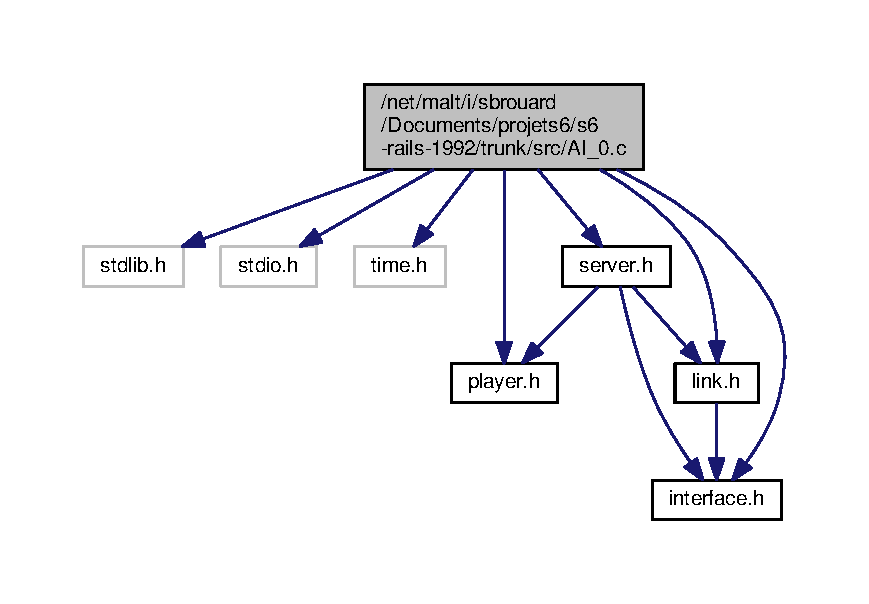
\includegraphics[width=350pt]{AI__0_8c__incl}
\end{center}
\end{figure}
\subsection*{Functions}
\begin{DoxyCompactItemize}
\item 
void \hyperlink{AI__0_8c_ae6a5a9fb92d4c61bff427f6d8964b1ce}{A\-I\-\_\-0\-\_\-fill\-\_\-tab\-\_\-accessible} (int $\ast$tab\-\_\-to\-\_\-fill, int current\-\_\-town, int id)
\begin{DoxyCompactList}\small\item\em A\-I\-\_\-0\-\_\-fill\-\_\-tab\-\_\-accessible (auxiliary function of the function \char`\"{}objective\-\_\-realised\char`\"{}) \end{DoxyCompactList}\item 
int \hyperlink{AI__0_8c_aca091cff3a4de4b7399735d192d204fc}{A\-I\-\_\-0\-\_\-objective\-\_\-realised} (int town1, int town2, int id)
\begin{DoxyCompactList}\small\item\em A\-I\-\_\-0\-\_\-objective\-\_\-realised. \end{DoxyCompactList}\item 
int \hyperlink{AI__0_8c_a4ed15e4ae5472f5bf9b586526318fcf3}{A\-I\-\_\-0\-\_\-init\-\_\-player} (int id, int nb\-\_\-players, int nb\-\_\-towns, int nb\-\_\-rails, struct \hyperlink{structRail}{Rail} $\ast$rails, int nb\-\_\-initial\-\_\-wagons, int nb\-\_\-obj, struct \hyperlink{structObjective}{Objective} $\ast$objs)
\begin{DoxyCompactList}\small\item\em A\-I\-\_\-0\-\_\-init\-\_\-player Initialises all the parameters of a struct \hyperlink{structPlayer}{Player} (composed of the general game parameters, and his own informations about the game). \end{DoxyCompactList}\item 
struct \hyperlink{structAction}{Action} \hyperlink{AI__0_8c_af51c2bc8672ee161b102e06843c3a045}{A\-I\-\_\-0\-\_\-play\-\_\-turn} (int $\ast$used\-\_\-wagons, int $\ast$cards\-\_\-in\-\_\-hand, int $\ast$objectives, int nb\-\_\-new\-\_\-rails, struct \hyperlink{structNew__rail}{New\-\_\-rail} $\ast$changes, int $\ast$new\-\_\-obj, int $\ast$cards)
\begin{DoxyCompactList}\small\item\em A\-I\-\_\-0\-\_\-play\-\_\-turn Calls the player, actualises all the changes that occured since the last time the player was called, and asks the player which action he wants. \end{DoxyCompactList}\item 
int $\ast$ \hyperlink{AI__0_8c_a776a149dd4b7d4685277ade0dd37c78a}{A\-I\-\_\-0\-\_\-choose\-\_\-objective} (int nb, int $\ast$objs, int min)
\begin{DoxyCompactList}\small\item\em A\-I\-\_\-0\-\_\-choose\-\_\-objective. \end{DoxyCompactList}\item 
int \hyperlink{AI__0_8c_aee5609d0a03a97567e6a828fbff34a7e}{A\-I\-\_\-0\-\_\-free\-\_\-player} ()
\begin{DoxyCompactList}\small\item\em A\-I\-\_\-0\-\_\-free\-\_\-player Frees the struct \hyperlink{structPlayer}{Player} of the player. \end{DoxyCompactList}\end{DoxyCompactItemize}


\subsection{Function Documentation}
\hypertarget{AI__0_8c_a776a149dd4b7d4685277ade0dd37c78a}{\index{A\-I\-\_\-0.\-c@{A\-I\-\_\-0.\-c}!A\-I\-\_\-0\-\_\-choose\-\_\-objective@{A\-I\-\_\-0\-\_\-choose\-\_\-objective}}
\index{A\-I\-\_\-0\-\_\-choose\-\_\-objective@{A\-I\-\_\-0\-\_\-choose\-\_\-objective}!AI_0.c@{A\-I\-\_\-0.\-c}}
\subsubsection[{A\-I\-\_\-0\-\_\-choose\-\_\-objective}]{\setlength{\rightskip}{0pt plus 5cm}int $\ast$ A\-I\-\_\-0\-\_\-choose\-\_\-objective (
\begin{DoxyParamCaption}
\item[{int}]{nb, }
\item[{int $\ast$}]{objs, }
\item[{int}]{min}
\end{DoxyParamCaption}
)}}\label{AI__0_8c_a776a149dd4b7d4685277ade0dd37c78a}


A\-I\-\_\-0\-\_\-choose\-\_\-objective. 


\begin{DoxyParams}{Parameters}
{\em nb} & is the number of objectives proposed to the player. \\
\hline
{\em objs} & is the tabular of the objectives proposed to the player. \\
\hline
{\em min} & is the minimum number of objectives that the player has to chose in the tabular \char`\"{}objs\char`\"{}. \\
\hline
\end{DoxyParams}
\begin{DoxyReturn}{Returns}
Returns a tabular (in the stack, but instantly registered by the server) indicating which objectives have been chosen. 
\end{DoxyReturn}


Here is the caller graph for this function\-:
\nopagebreak
\begin{figure}[H]
\begin{center}
\leavevmode
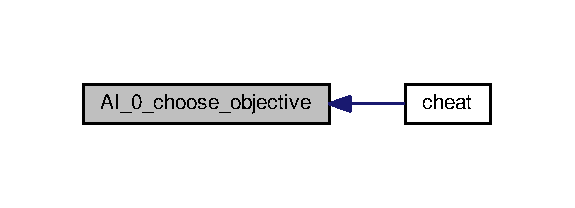
\includegraphics[width=276pt]{AI__0_8c_a776a149dd4b7d4685277ade0dd37c78a_icgraph}
\end{center}
\end{figure}


\hypertarget{AI__0_8c_ae6a5a9fb92d4c61bff427f6d8964b1ce}{\index{A\-I\-\_\-0.\-c@{A\-I\-\_\-0.\-c}!A\-I\-\_\-0\-\_\-fill\-\_\-tab\-\_\-accessible@{A\-I\-\_\-0\-\_\-fill\-\_\-tab\-\_\-accessible}}
\index{A\-I\-\_\-0\-\_\-fill\-\_\-tab\-\_\-accessible@{A\-I\-\_\-0\-\_\-fill\-\_\-tab\-\_\-accessible}!AI_0.c@{A\-I\-\_\-0.\-c}}
\subsubsection[{A\-I\-\_\-0\-\_\-fill\-\_\-tab\-\_\-accessible}]{\setlength{\rightskip}{0pt plus 5cm}void A\-I\-\_\-0\-\_\-fill\-\_\-tab\-\_\-accessible (
\begin{DoxyParamCaption}
\item[{int $\ast$}]{tab\-\_\-to\-\_\-fill, }
\item[{int}]{current\-\_\-town, }
\item[{int}]{id}
\end{DoxyParamCaption}
)}}\label{AI__0_8c_ae6a5a9fb92d4c61bff427f6d8964b1ce}


A\-I\-\_\-0\-\_\-fill\-\_\-tab\-\_\-accessible (auxiliary function of the function \char`\"{}objective\-\_\-realised\char`\"{}) 


\begin{DoxyParams}{Parameters}
{\em tab\-\_\-to\-\_\-fill} & is a tabular of size the total number of towns; the function is going to set tab\-\_\-to\-\_\-fill\mbox{[}i\mbox{]} at 1 if the town \char`\"{}i\char`\"{} is accessible by the player from the town \char`\"{}current\-\_\-town\char`\"{}. \\
\hline
{\em current\-\_\-town} & is the town from which the function is going to search all towns accessible by the player (if he has set a rails from this town); at the begining\-: current\-\_\-town=town1 or town2 of the objective \\
\hline
{\em id} & is the identifier of the player. \\
\hline
\end{DoxyParams}


Here is the call graph for this function\-:
\nopagebreak
\begin{figure}[H]
\begin{center}
\leavevmode
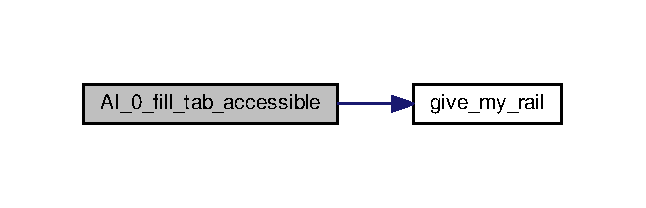
\includegraphics[width=310pt]{AI__0_8c_ae6a5a9fb92d4c61bff427f6d8964b1ce_cgraph}
\end{center}
\end{figure}




Here is the caller graph for this function\-:
\nopagebreak
\begin{figure}[H]
\begin{center}
\leavevmode
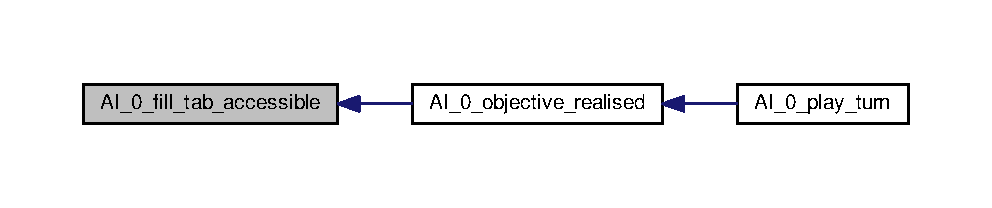
\includegraphics[width=350pt]{AI__0_8c_ae6a5a9fb92d4c61bff427f6d8964b1ce_icgraph}
\end{center}
\end{figure}


\hypertarget{AI__0_8c_aee5609d0a03a97567e6a828fbff34a7e}{\index{A\-I\-\_\-0.\-c@{A\-I\-\_\-0.\-c}!A\-I\-\_\-0\-\_\-free\-\_\-player@{A\-I\-\_\-0\-\_\-free\-\_\-player}}
\index{A\-I\-\_\-0\-\_\-free\-\_\-player@{A\-I\-\_\-0\-\_\-free\-\_\-player}!AI_0.c@{A\-I\-\_\-0.\-c}}
\subsubsection[{A\-I\-\_\-0\-\_\-free\-\_\-player}]{\setlength{\rightskip}{0pt plus 5cm}int A\-I\-\_\-0\-\_\-free\-\_\-player (
\begin{DoxyParamCaption}
{}
\end{DoxyParamCaption}
)}}\label{AI__0_8c_aee5609d0a03a97567e6a828fbff34a7e}


A\-I\-\_\-0\-\_\-free\-\_\-player Frees the struct \hyperlink{structPlayer}{Player} of the player. 

\begin{DoxyReturn}{Returns}
Returns 1 if the player has been freed well. 
\end{DoxyReturn}


Here is the caller graph for this function\-:
\nopagebreak
\begin{figure}[H]
\begin{center}
\leavevmode
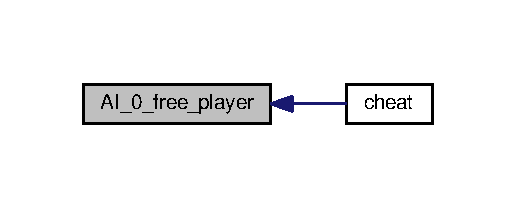
\includegraphics[width=248pt]{AI__0_8c_aee5609d0a03a97567e6a828fbff34a7e_icgraph}
\end{center}
\end{figure}


\hypertarget{AI__0_8c_a4ed15e4ae5472f5bf9b586526318fcf3}{\index{A\-I\-\_\-0.\-c@{A\-I\-\_\-0.\-c}!A\-I\-\_\-0\-\_\-init\-\_\-player@{A\-I\-\_\-0\-\_\-init\-\_\-player}}
\index{A\-I\-\_\-0\-\_\-init\-\_\-player@{A\-I\-\_\-0\-\_\-init\-\_\-player}!AI_0.c@{A\-I\-\_\-0.\-c}}
\subsubsection[{A\-I\-\_\-0\-\_\-init\-\_\-player}]{\setlength{\rightskip}{0pt plus 5cm}int A\-I\-\_\-0\-\_\-init\-\_\-player (
\begin{DoxyParamCaption}
\item[{int}]{id, }
\item[{int}]{nb\-\_\-players, }
\item[{int}]{nb\-\_\-towns, }
\item[{int}]{nb\-\_\-rails, }
\item[{struct {\bf Rail} $\ast$}]{rails, }
\item[{int}]{nb\-\_\-initial\-\_\-wagons, }
\item[{int}]{nb\-\_\-obj, }
\item[{struct {\bf Objective} $\ast$}]{objs}
\end{DoxyParamCaption}
)}}\label{AI__0_8c_a4ed15e4ae5472f5bf9b586526318fcf3}


A\-I\-\_\-0\-\_\-init\-\_\-player Initialises all the parameters of a struct \hyperlink{structPlayer}{Player} (composed of the general game parameters, and his own informations about the game). 


\begin{DoxyParams}{Parameters}
{\em id} & is the identifier of the player. \\
\hline
{\em nb\-\_\-players} & is the total number of players in the game. \\
\hline
{\em nb\-\_\-towns} & is the total number of towns in the game. \\
\hline
{\em nb\-\_\-rails} & is the total number of rails in the game. \\
\hline
{\em rails} & is the tabular composed of all the rails of the game. \\
\hline
{\em nb\-\_\-initial\-\_\-wagons} & is the number of wagons that each player has at the begining of the game. \\
\hline
{\em nb\-\_\-obj} & is the total number of objective-\/cards of the game. \\
\hline
{\em objs} & is the tabular composed of all the objective-\/cards of the game. \\
\hline
\end{DoxyParams}
\begin{DoxyReturn}{Returns}
Returns 1 if the initialisation went well; 0 otherwise. 
\end{DoxyReturn}


Here is the call graph for this function\-:
\nopagebreak
\begin{figure}[H]
\begin{center}
\leavevmode
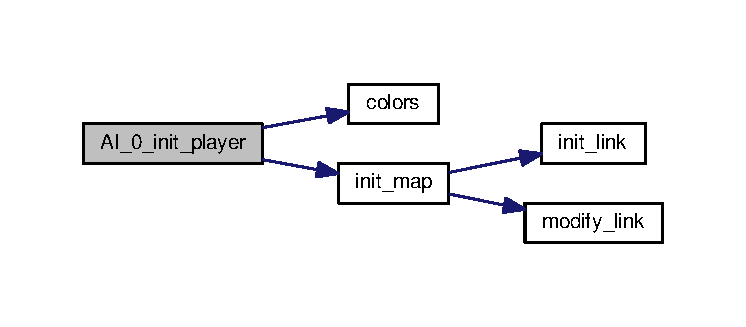
\includegraphics[width=350pt]{AI__0_8c_a4ed15e4ae5472f5bf9b586526318fcf3_cgraph}
\end{center}
\end{figure}




Here is the caller graph for this function\-:
\nopagebreak
\begin{figure}[H]
\begin{center}
\leavevmode
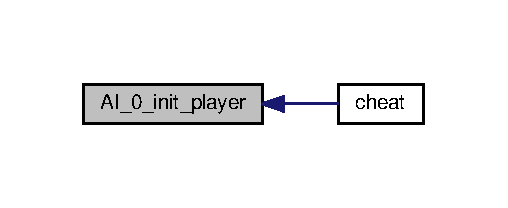
\includegraphics[width=244pt]{AI__0_8c_a4ed15e4ae5472f5bf9b586526318fcf3_icgraph}
\end{center}
\end{figure}


\hypertarget{AI__0_8c_aca091cff3a4de4b7399735d192d204fc}{\index{A\-I\-\_\-0.\-c@{A\-I\-\_\-0.\-c}!A\-I\-\_\-0\-\_\-objective\-\_\-realised@{A\-I\-\_\-0\-\_\-objective\-\_\-realised}}
\index{A\-I\-\_\-0\-\_\-objective\-\_\-realised@{A\-I\-\_\-0\-\_\-objective\-\_\-realised}!AI_0.c@{A\-I\-\_\-0.\-c}}
\subsubsection[{A\-I\-\_\-0\-\_\-objective\-\_\-realised}]{\setlength{\rightskip}{0pt plus 5cm}int A\-I\-\_\-0\-\_\-objective\-\_\-realised (
\begin{DoxyParamCaption}
\item[{int}]{town1, }
\item[{int}]{town2, }
\item[{int}]{id}
\end{DoxyParamCaption}
)}}\label{AI__0_8c_aca091cff3a4de4b7399735d192d204fc}


A\-I\-\_\-0\-\_\-objective\-\_\-realised. 


\begin{DoxyParams}{Parameters}
{\em town1} & is the town1 of the objective. \\
\hline
{\em town2} & is the town2 of the objective. \\
\hline
{\em id} & is the identifier of a given player. \\
\hline
\end{DoxyParams}
\begin{DoxyReturn}{Returns}
Returns 1 if the objective has been realised by the player. 
\end{DoxyReturn}


Here is the call graph for this function\-:
\nopagebreak
\begin{figure}[H]
\begin{center}
\leavevmode
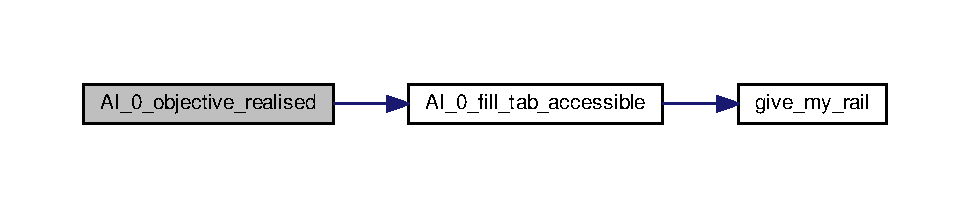
\includegraphics[width=350pt]{AI__0_8c_aca091cff3a4de4b7399735d192d204fc_cgraph}
\end{center}
\end{figure}




Here is the caller graph for this function\-:
\nopagebreak
\begin{figure}[H]
\begin{center}
\leavevmode
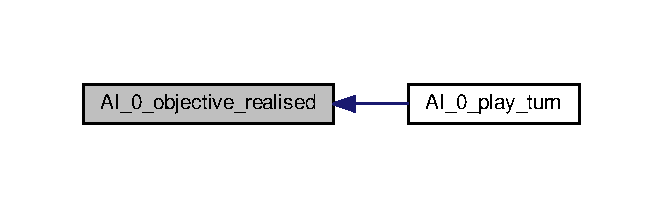
\includegraphics[width=318pt]{AI__0_8c_aca091cff3a4de4b7399735d192d204fc_icgraph}
\end{center}
\end{figure}


\hypertarget{AI__0_8c_af51c2bc8672ee161b102e06843c3a045}{\index{A\-I\-\_\-0.\-c@{A\-I\-\_\-0.\-c}!A\-I\-\_\-0\-\_\-play\-\_\-turn@{A\-I\-\_\-0\-\_\-play\-\_\-turn}}
\index{A\-I\-\_\-0\-\_\-play\-\_\-turn@{A\-I\-\_\-0\-\_\-play\-\_\-turn}!AI_0.c@{A\-I\-\_\-0.\-c}}
\subsubsection[{A\-I\-\_\-0\-\_\-play\-\_\-turn}]{\setlength{\rightskip}{0pt plus 5cm}struct {\bf Action} A\-I\-\_\-0\-\_\-play\-\_\-turn (
\begin{DoxyParamCaption}
\item[{int $\ast$}]{used\-\_\-wagons, }
\item[{int $\ast$}]{cards\-\_\-in\-\_\-hand, }
\item[{int $\ast$}]{objectives, }
\item[{int}]{nb\-\_\-new\-\_\-rails, }
\item[{struct {\bf New\-\_\-rail} $\ast$}]{changes, }
\item[{int $\ast$}]{new\-\_\-obj, }
\item[{int $\ast$}]{cards}
\end{DoxyParamCaption}
)}}\label{AI__0_8c_af51c2bc8672ee161b102e06843c3a045}


A\-I\-\_\-0\-\_\-play\-\_\-turn Calls the player, actualises all the changes that occured since the last time the player was called, and asks the player which action he wants. 


\begin{DoxyParams}{Parameters}
{\em used\-\_\-wagons} & is a tabular which length is the number of players (for a given player, the tabular's value is the number of wagons he has set during the last round). \\
\hline
{\em cards\-\_\-in\-\_\-hand} & is a tabular which length is the number of players (for a given player, the tabular's value is the number of cards that the player has won or lost during the last round\-: negative if lost). \\
\hline
{\em objectives} & is a tabular composed of the number of objectives drawned by each player. \\
\hline
{\em nb\-\_\-new\-\_\-rails} & is the length of the tabular changes (= the number of rails that the current player has set during the last round). \\
\hline
{\em changes} & is the tabular of all the rails that the players have set during the last round. \\
\hline
{\em new\-\_\-obj} & is the tabular of the objectives that the current player has drawned during the last round. \\
\hline
{\em cards} & If the action chosen in the last round was \char`\"{}draw\char`\"{}\-: \char`\"{}cards\char`\"{} is the tabular of all the colors (= wagon-\/cards) drawned. If the action chosen was \char`\"{}build\char`\"{}\-: \char`\"{}cards\char`\"{} is the tabular of all the colors lost (because set). \\
\hline
\end{DoxyParams}
\begin{DoxyReturn}{Returns}
Returns the struct \hyperlink{structAction}{Action} chosen and completed by the player according to his strategy. 
\end{DoxyReturn}


Here is the call graph for this function\-:
\nopagebreak
\begin{figure}[H]
\begin{center}
\leavevmode
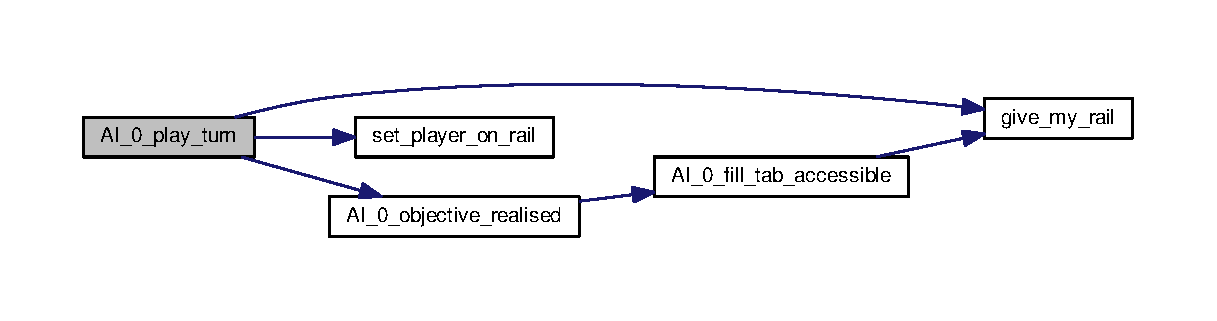
\includegraphics[width=350pt]{AI__0_8c_af51c2bc8672ee161b102e06843c3a045_cgraph}
\end{center}
\end{figure}



\hypertarget{AI__1_8c}{\section{/net/malt/i/sbrouard/\-Documents/projets6/s6-\/rails-\/1992/trunk/src/\-A\-I\-\_\-1.c File Reference}
\label{AI__1_8c}\index{/net/malt/i/sbrouard/\-Documents/projets6/s6-\/rails-\/1992/trunk/src/\-A\-I\-\_\-1.\-c@{/net/malt/i/sbrouard/\-Documents/projets6/s6-\/rails-\/1992/trunk/src/\-A\-I\-\_\-1.\-c}}
}
{\ttfamily \#include \char`\"{}player.\-h\char`\"{}}\\*
{\ttfamily \#include \char`\"{}link.\-h\char`\"{}}\\*
{\ttfamily \#include \char`\"{}interface.\-h\char`\"{}}\\*
{\ttfamily \#include \char`\"{}server.\-h\char`\"{}}\\*
{\ttfamily \#include $<$stdio.\-h$>$}\\*
{\ttfamily \#include $<$stdlib.\-h$>$}\\*
Include dependency graph for A\-I\-\_\-1.\-c\-:
\nopagebreak
\begin{figure}[H]
\begin{center}
\leavevmode
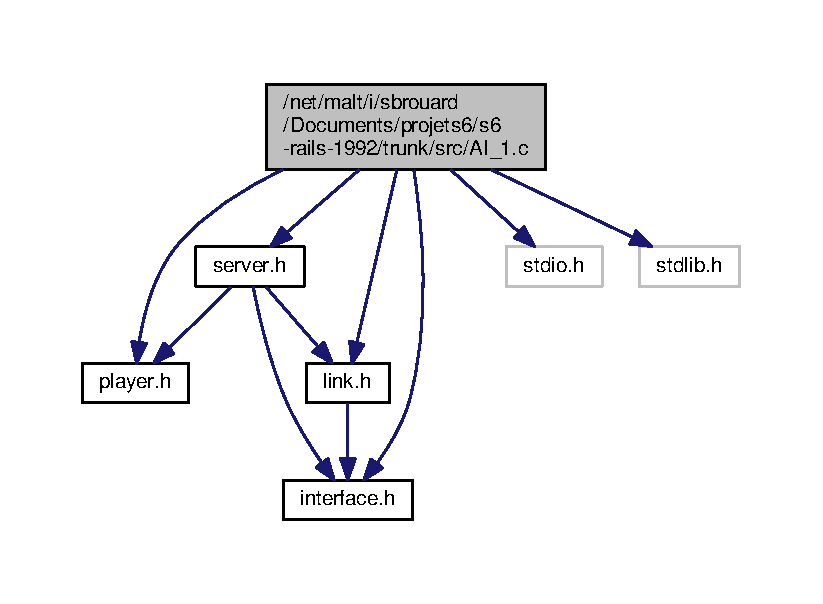
\includegraphics[width=350pt]{AI__1_8c__incl}
\end{center}
\end{figure}
\subsection*{Functions}
\begin{DoxyCompactItemize}
\item 
int \hyperlink{AI__1_8c_a1795878e593a98deac75d49b176d5591}{give\-\_\-size\-\_\-accessible\-\_\-rails} (struct \hyperlink{structRail}{Rail} $\ast$tab, int size, int id)
\begin{DoxyCompactList}\small\item\em give\-\_\-size\-\_\-accessible\-\_\-rails \end{DoxyCompactList}\item 
void \hyperlink{AI__1_8c_ac8b1940d56dd92a1ec206747bd3846c6}{accessible\-\_\-rails} (struct \hyperlink{structRail}{Rail} $\ast$tab, int $\ast$tab\-\_\-indices, int size, int id)
\begin{DoxyCompactList}\small\item\em accessible\-\_\-rails \end{DoxyCompactList}\item 
void \hyperlink{AI__1_8c_ac3468cbfd5d55ca81b2d1f65c77263c3}{sort\-\_\-length} (struct \hyperlink{structRail}{Rail} $\ast$tab, int $\ast$tab\-\_\-indices, int size)
\begin{DoxyCompactList}\small\item\em sort\-\_\-length \end{DoxyCompactList}\item 
void \hyperlink{AI__1_8c_a059af6cb848a8b0392218ef6d97a0a87}{A\-I\-\_\-1\-\_\-fill\-\_\-tab\-\_\-accessible} (int $\ast$tab\-\_\-to\-\_\-fill, int current\-\_\-town, int id)
\begin{DoxyCompactList}\small\item\em A\-I\-\_\-1\-\_\-fill\-\_\-tab\-\_\-accessible (auxiliary function of the function \char`\"{}objective\-\_\-realised\char`\"{}) \end{DoxyCompactList}\item 
int \hyperlink{AI__1_8c_ad92748bc33ab88fa6ea22a4da3ac71fc}{A\-I\-\_\-1\-\_\-objective\-\_\-realised} (int town1, int town2, int id)
\begin{DoxyCompactList}\small\item\em A\-I\-\_\-1\-\_\-objective\-\_\-realised. \end{DoxyCompactList}\item 
void \hyperlink{AI__1_8c_a44afa06d0ad3e478f1046db37fffb663}{actualise\-\_\-all\-\_\-parameters\-\_\-received} (int $\ast$used\-\_\-wagons, int $\ast$cards\-\_\-in\-\_\-hand, int $\ast$objectives, int nb\-\_\-new\-\_\-rails, struct \hyperlink{structNew__rail}{New\-\_\-rail} $\ast$changes, int $\ast$new\-\_\-obj, int $\ast$cards)
\begin{DoxyCompactList}\small\item\em actualise\-\_\-all\-\_\-parameters\-\_\-received Actualises all the changes that occured since the last time the player was called. \end{DoxyCompactList}\item 
void \hyperlink{AI__1_8c_a72603999060857e266eeb57fe4651028}{fill\-\_\-tab\-\_\-acyclic} (struct \hyperlink{structRail}{Rail} $\ast$tab, int size, int $\ast$tab\-\_\-to\-\_\-fill, int current\-\_\-town)
\begin{DoxyCompactList}\small\item\em fill\-\_\-tab\-\_\-acyclic Is a recursive function which fills the tabular \char`\"{}tab\-\_\-to\-\_\-fill\char`\"{} (set the indice \char`\"{}i\char`\"{} at 1 if the town \char`\"{}i\char`\"{} is accessible from the town \char`\"{}current\-\_\-town\char`\"{} by using rails of the tabular \char`\"{}tab\char`\"{}, 0 otherwise). \end{DoxyCompactList}\item 
int \hyperlink{AI__1_8c_a44c081878b0293e9b15eca36357a9731}{acyclic} (struct \hyperlink{structRail}{Rail} $\ast$tab, int size, struct \hyperlink{structRail}{Rail} rail)
\begin{DoxyCompactList}\small\item\em acyclic \end{DoxyCompactList}\item 
int \hyperlink{AI__1_8c_a570906173de0ecea152cada5a76f8a44}{fill\-\_\-tab\-\_\-rail\-\_\-free\-\_\-in\-\_\-\-A\-C\-M} (struct \hyperlink{structRail}{Rail} $\ast$tab, int $\ast$acm\-\_\-tab\-\_\-indices, int size, int $\ast$tab\-\_\-towns\-\_\-to\-\_\-fill, int $\ast$tab\-\_\-rails\-\_\-to\-\_\-fill, int current\-\_\-town, int town\-\_\-to\-\_\-reach)
\begin{DoxyCompactList}\small\item\em fill\-\_\-tab\-\_\-rail\-\_\-free\-\_\-in\-\_\-\-A\-C\-M \end{DoxyCompactList}\item 
int \hyperlink{AI__1_8c_ab12b4fcf8835504e67cc690b905a6e3c}{rail\-\_\-free\-\_\-in\-\_\-\-A\-C\-M} (struct \hyperlink{structRail}{Rail} $\ast$acm, int $\ast$acm\-\_\-tab\-\_\-indices, int size, int town1, int town2)
\begin{DoxyCompactList}\small\item\em rail\-\_\-free\-\_\-in\-\_\-\-A\-C\-M \end{DoxyCompactList}\item 
int \hyperlink{AI__1_8c_a4b129a9daa97da56708afe7568021aa1}{A\-I\-\_\-1\-\_\-init\-\_\-player} (int id, int nb\-\_\-players, int nb\-\_\-towns, int nb\-\_\-rails, struct \hyperlink{structRail}{Rail} $\ast$rails, int nb\-\_\-initial\-\_\-wagons, int nb\-\_\-obj, struct \hyperlink{structObjective}{Objective} $\ast$objs)
\begin{DoxyCompactList}\small\item\em A\-I\-\_\-0\-\_\-init\-\_\-player Initialises all the parameters of a struct \hyperlink{structPlayer}{Player} (composed of the general game parameters, and his own informations about the game). \end{DoxyCompactList}\item 
struct \hyperlink{structAction}{Action} \hyperlink{AI__1_8c_a8f776e760f32f938ce3203363f807f35}{A\-I\-\_\-1\-\_\-play\-\_\-turn} (int $\ast$used\-\_\-wagons, int $\ast$cards\-\_\-in\-\_\-hand, int $\ast$objectives, int nb\-\_\-new\-\_\-rails, struct \hyperlink{structNew__rail}{New\-\_\-rail} $\ast$changes, int $\ast$new\-\_\-obj, int $\ast$cards)
\begin{DoxyCompactList}\small\item\em A\-I\-\_\-0\-\_\-play\-\_\-turn Calls the player, actualises all the changes that occured since the last time the player was called, and asks the player which action he wants. \end{DoxyCompactList}\item 
int \hyperlink{AI__1_8c_aa14010606b2c569bd491a7101a020023}{min\-\_\-point\-\_\-objs} (int nb, int $\ast$objs, int $\ast$tab)
\begin{DoxyCompactList}\small\item\em min\-\_\-point\-\_\-objs \end{DoxyCompactList}\item 
int $\ast$ \hyperlink{AI__1_8c_a48809ba554faa1bf2ef2118392330ae2}{A\-I\-\_\-1\-\_\-choose\-\_\-objective} (int nb, int $\ast$objs, int min)
\begin{DoxyCompactList}\small\item\em A\-I\-\_\-0\-\_\-choose\-\_\-objective. \end{DoxyCompactList}\item 
int \hyperlink{AI__1_8c_a064e38e8072edd14b0bef80985ddd412}{A\-I\-\_\-1\-\_\-free\-\_\-player} ()
\begin{DoxyCompactList}\small\item\em A\-I\-\_\-0\-\_\-free\-\_\-player Frees the struct \hyperlink{structPlayer}{Player} of the player. \end{DoxyCompactList}\end{DoxyCompactItemize}
\subsection*{Variables}
\begin{DoxyCompactItemize}
\item 
struct \hyperlink{structPlayer}{Player} \hyperlink{AI__1_8c_a47a2d030ed3cc6ecfbb6afd9a65b7869}{A\-I\-\_\-1}
\end{DoxyCompactItemize}


\subsection{Function Documentation}
\hypertarget{AI__1_8c_ac8b1940d56dd92a1ec206747bd3846c6}{\index{A\-I\-\_\-1.\-c@{A\-I\-\_\-1.\-c}!accessible\-\_\-rails@{accessible\-\_\-rails}}
\index{accessible\-\_\-rails@{accessible\-\_\-rails}!AI_1.c@{A\-I\-\_\-1.\-c}}
\subsubsection[{accessible\-\_\-rails}]{\setlength{\rightskip}{0pt plus 5cm}void accessible\-\_\-rails (
\begin{DoxyParamCaption}
\item[{struct {\bf Rail} $\ast$}]{tab, }
\item[{int $\ast$}]{tab\-\_\-indices, }
\item[{int}]{size, }
\item[{int}]{id}
\end{DoxyParamCaption}
)}}\label{AI__1_8c_ac8b1940d56dd92a1ec206747bd3846c6}


accessible\-\_\-rails 


\begin{DoxyParams}{Parameters}
{\em tab} & is the tabular of struct Rails from which the function is going to keep the still accessible rails and the rails already owned by the given player. \\
\hline
{\em tab\-\_\-indices} & is the tabular that the function is going to fill (if struct \hyperlink{structRail}{Rail} at indice \char`\"{}i\char`\"{} is kept, tab\-\_\-indices\mbox{[}i\mbox{]}=1, 0 otherwise). \\
\hline
{\em size} & is the length of the tabular \char`\"{}tab\char`\"{}. \\
\hline
{\em id} & is the identifier of a given player. \\
\hline
\end{DoxyParams}


Here is the call graph for this function\-:
\nopagebreak
\begin{figure}[H]
\begin{center}
\leavevmode
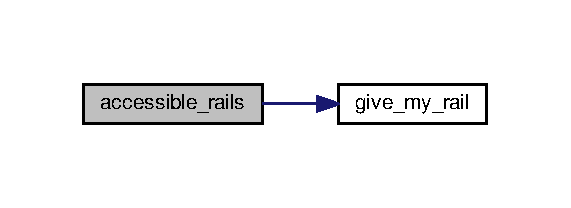
\includegraphics[width=274pt]{AI__1_8c_ac8b1940d56dd92a1ec206747bd3846c6_cgraph}
\end{center}
\end{figure}




Here is the caller graph for this function\-:
\nopagebreak
\begin{figure}[H]
\begin{center}
\leavevmode
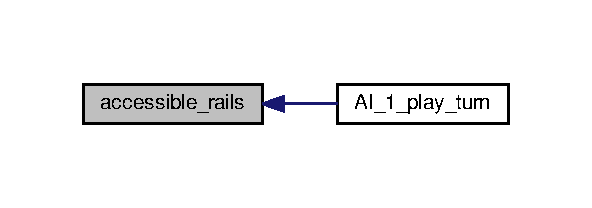
\includegraphics[width=284pt]{AI__1_8c_ac8b1940d56dd92a1ec206747bd3846c6_icgraph}
\end{center}
\end{figure}


\hypertarget{AI__1_8c_a44afa06d0ad3e478f1046db37fffb663}{\index{A\-I\-\_\-1.\-c@{A\-I\-\_\-1.\-c}!actualise\-\_\-all\-\_\-parameters\-\_\-received@{actualise\-\_\-all\-\_\-parameters\-\_\-received}}
\index{actualise\-\_\-all\-\_\-parameters\-\_\-received@{actualise\-\_\-all\-\_\-parameters\-\_\-received}!AI_1.c@{A\-I\-\_\-1.\-c}}
\subsubsection[{actualise\-\_\-all\-\_\-parameters\-\_\-received}]{\setlength{\rightskip}{0pt plus 5cm}void actualise\-\_\-all\-\_\-parameters\-\_\-received (
\begin{DoxyParamCaption}
\item[{int $\ast$}]{used\-\_\-wagons, }
\item[{int $\ast$}]{cards\-\_\-in\-\_\-hand, }
\item[{int $\ast$}]{objectives, }
\item[{int}]{nb\-\_\-new\-\_\-rails, }
\item[{struct {\bf New\-\_\-rail} $\ast$}]{changes, }
\item[{int $\ast$}]{new\-\_\-obj, }
\item[{int $\ast$}]{cards}
\end{DoxyParamCaption}
)}}\label{AI__1_8c_a44afa06d0ad3e478f1046db37fffb663}


actualise\-\_\-all\-\_\-parameters\-\_\-received Actualises all the changes that occured since the last time the player was called. 


\begin{DoxyParams}{Parameters}
{\em used\-\_\-wagons} & is a tabular which length is the number of players (for a given player, the tabular's value is the number of wagons he has set during the last round). \\
\hline
{\em cards\-\_\-in\-\_\-hand} & is a tabular which length is the number of players (for a given player, the tabular's value is the number of cards that the player has won or lost during the last round). \\
\hline
{\em objectives} & is a tabular composed of the number of objectives drawned by each player. \\
\hline
{\em nb\-\_\-new\-\_\-rails} & is the length of the tabular changes (= the number of rails that the current player has set during the last round). \\
\hline
{\em changes} & is the tabular of all the rails that the current player has set during the last round. \\
\hline
{\em new\-\_\-obj} & is the tabular of the objectives that the current player has drawned during the last round. \\
\hline
{\em cards} & If the action chosen in the last round was \char`\"{}draw\char`\"{}\-: \char`\"{}cards\char`\"{} is the tabuler of all the colors (= wagon-\/cards) drawned. If the action chosen was \char`\"{}build\char`\"{}\-: \char`\"{}cards\char`\"{} is the tabular of all the colors lost (because set). \\
\hline
\end{DoxyParams}


Here is the call graph for this function\-:
\nopagebreak
\begin{figure}[H]
\begin{center}
\leavevmode
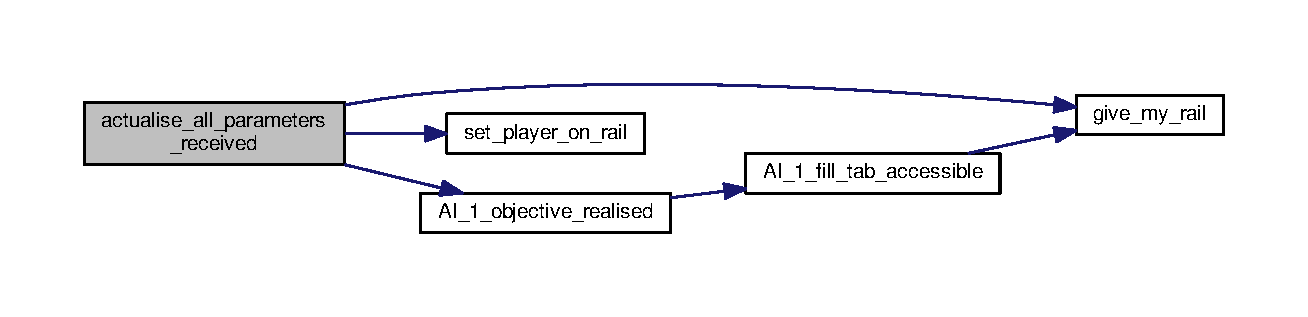
\includegraphics[width=350pt]{AI__1_8c_a44afa06d0ad3e478f1046db37fffb663_cgraph}
\end{center}
\end{figure}




Here is the caller graph for this function\-:
\nopagebreak
\begin{figure}[H]
\begin{center}
\leavevmode
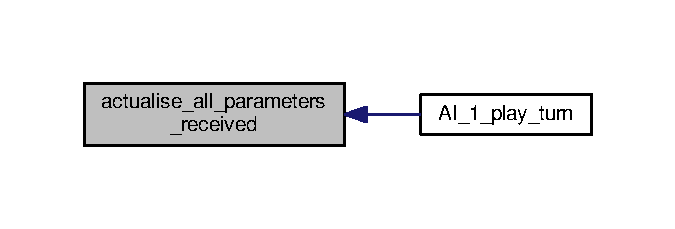
\includegraphics[width=324pt]{AI__1_8c_a44afa06d0ad3e478f1046db37fffb663_icgraph}
\end{center}
\end{figure}


\hypertarget{AI__1_8c_a44c081878b0293e9b15eca36357a9731}{\index{A\-I\-\_\-1.\-c@{A\-I\-\_\-1.\-c}!acyclic@{acyclic}}
\index{acyclic@{acyclic}!AI_1.c@{A\-I\-\_\-1.\-c}}
\subsubsection[{acyclic}]{\setlength{\rightskip}{0pt plus 5cm}int acyclic (
\begin{DoxyParamCaption}
\item[{struct {\bf Rail} $\ast$}]{tab, }
\item[{int}]{size, }
\item[{struct {\bf Rail}}]{rail}
\end{DoxyParamCaption}
)}}\label{AI__1_8c_a44c081878b0293e9b15eca36357a9731}


acyclic 


\begin{DoxyParams}{Parameters}
{\em tab} & is a tabular of struct Rails which correspond to a certain number of rails which represent an acyclic graph. \\
\hline
{\em size} & is the length of the tabular \char`\"{}tab\char`\"{}. \\
\hline
{\em rail} & is a rail which is not already in the tabular \char`\"{}tab\char`\"{}. \\
\hline
\end{DoxyParams}
\begin{DoxyReturn}{Returns}
Returns 1 if all the rails of the tabular \char`\"{}tab\char`\"{} plus the rail \char`\"{}rail\char`\"{} represent an acyclic graph. 
\end{DoxyReturn}


Here is the call graph for this function\-:
\nopagebreak
\begin{figure}[H]
\begin{center}
\leavevmode
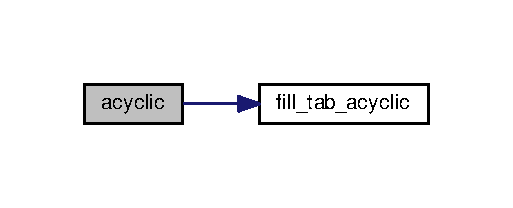
\includegraphics[width=246pt]{AI__1_8c_a44c081878b0293e9b15eca36357a9731_cgraph}
\end{center}
\end{figure}




Here is the caller graph for this function\-:
\nopagebreak
\begin{figure}[H]
\begin{center}
\leavevmode
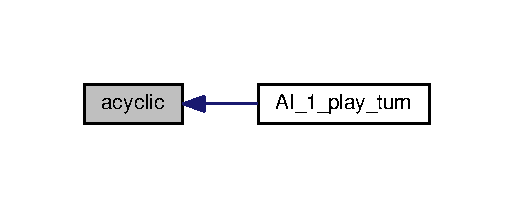
\includegraphics[width=246pt]{AI__1_8c_a44c081878b0293e9b15eca36357a9731_icgraph}
\end{center}
\end{figure}


\hypertarget{AI__1_8c_a48809ba554faa1bf2ef2118392330ae2}{\index{A\-I\-\_\-1.\-c@{A\-I\-\_\-1.\-c}!A\-I\-\_\-1\-\_\-choose\-\_\-objective@{A\-I\-\_\-1\-\_\-choose\-\_\-objective}}
\index{A\-I\-\_\-1\-\_\-choose\-\_\-objective@{A\-I\-\_\-1\-\_\-choose\-\_\-objective}!AI_1.c@{A\-I\-\_\-1.\-c}}
\subsubsection[{A\-I\-\_\-1\-\_\-choose\-\_\-objective}]{\setlength{\rightskip}{0pt plus 5cm}int $\ast$ A\-I\-\_\-1\-\_\-choose\-\_\-objective (
\begin{DoxyParamCaption}
\item[{int}]{nb, }
\item[{int $\ast$}]{objs, }
\item[{int}]{min}
\end{DoxyParamCaption}
)}}\label{AI__1_8c_a48809ba554faa1bf2ef2118392330ae2}


A\-I\-\_\-0\-\_\-choose\-\_\-objective. 


\begin{DoxyParams}{Parameters}
{\em nb} & is the number of objectives proposed to the player. \\
\hline
{\em objs} & is the tabular of the objectives proposed to the player. \\
\hline
{\em min} & is the minimum number of objectives that the player has to chose in the tabular \char`\"{}objs\char`\"{}. \\
\hline
\end{DoxyParams}
\begin{DoxyReturn}{Returns}
Returns a tabular (in the stack, but instantly registered by the server) indicating which objectives have been chosen. 
\end{DoxyReturn}


Here is the call graph for this function\-:
\nopagebreak
\begin{figure}[H]
\begin{center}
\leavevmode
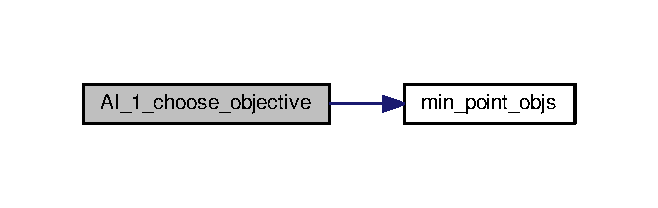
\includegraphics[width=316pt]{AI__1_8c_a48809ba554faa1bf2ef2118392330ae2_cgraph}
\end{center}
\end{figure}




Here is the caller graph for this function\-:
\nopagebreak
\begin{figure}[H]
\begin{center}
\leavevmode
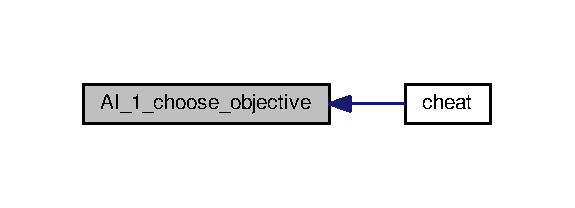
\includegraphics[width=276pt]{AI__1_8c_a48809ba554faa1bf2ef2118392330ae2_icgraph}
\end{center}
\end{figure}


\hypertarget{AI__1_8c_a059af6cb848a8b0392218ef6d97a0a87}{\index{A\-I\-\_\-1.\-c@{A\-I\-\_\-1.\-c}!A\-I\-\_\-1\-\_\-fill\-\_\-tab\-\_\-accessible@{A\-I\-\_\-1\-\_\-fill\-\_\-tab\-\_\-accessible}}
\index{A\-I\-\_\-1\-\_\-fill\-\_\-tab\-\_\-accessible@{A\-I\-\_\-1\-\_\-fill\-\_\-tab\-\_\-accessible}!AI_1.c@{A\-I\-\_\-1.\-c}}
\subsubsection[{A\-I\-\_\-1\-\_\-fill\-\_\-tab\-\_\-accessible}]{\setlength{\rightskip}{0pt plus 5cm}void A\-I\-\_\-1\-\_\-fill\-\_\-tab\-\_\-accessible (
\begin{DoxyParamCaption}
\item[{int $\ast$}]{tab\-\_\-to\-\_\-fill, }
\item[{int}]{current\-\_\-town, }
\item[{int}]{id}
\end{DoxyParamCaption}
)}}\label{AI__1_8c_a059af6cb848a8b0392218ef6d97a0a87}


A\-I\-\_\-1\-\_\-fill\-\_\-tab\-\_\-accessible (auxiliary function of the function \char`\"{}objective\-\_\-realised\char`\"{}) 


\begin{DoxyParams}{Parameters}
{\em tab\-\_\-to\-\_\-fill} & is a tabular of size the total number of towns; the function is going to set tab\-\_\-to\-\_\-fill\mbox{[}i\mbox{]} at 1 if the town \char`\"{}i\char`\"{} is accessible by the player from the town \char`\"{}current\-\_\-town\char`\"{}. \\
\hline
{\em current\-\_\-town} & is the town from which the function is going to search all towns accessible by the player (if he has set a rails from this town); at the begining\-: current\-\_\-town=town1 or town2 of the objective \\
\hline
{\em id} & is the identifier of the player. \\
\hline
\end{DoxyParams}


Here is the call graph for this function\-:
\nopagebreak
\begin{figure}[H]
\begin{center}
\leavevmode
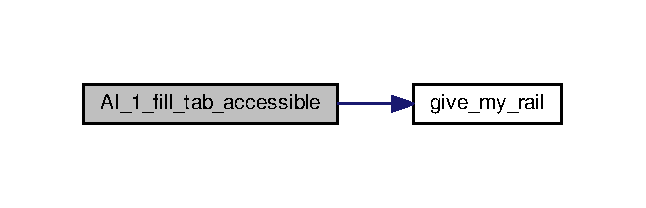
\includegraphics[width=310pt]{AI__1_8c_a059af6cb848a8b0392218ef6d97a0a87_cgraph}
\end{center}
\end{figure}




Here is the caller graph for this function\-:
\nopagebreak
\begin{figure}[H]
\begin{center}
\leavevmode
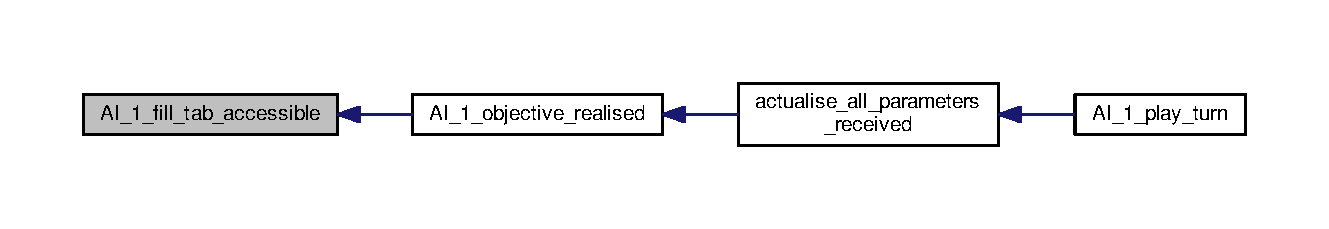
\includegraphics[width=350pt]{AI__1_8c_a059af6cb848a8b0392218ef6d97a0a87_icgraph}
\end{center}
\end{figure}


\hypertarget{AI__1_8c_a064e38e8072edd14b0bef80985ddd412}{\index{A\-I\-\_\-1.\-c@{A\-I\-\_\-1.\-c}!A\-I\-\_\-1\-\_\-free\-\_\-player@{A\-I\-\_\-1\-\_\-free\-\_\-player}}
\index{A\-I\-\_\-1\-\_\-free\-\_\-player@{A\-I\-\_\-1\-\_\-free\-\_\-player}!AI_1.c@{A\-I\-\_\-1.\-c}}
\subsubsection[{A\-I\-\_\-1\-\_\-free\-\_\-player}]{\setlength{\rightskip}{0pt plus 5cm}int A\-I\-\_\-1\-\_\-free\-\_\-player (
\begin{DoxyParamCaption}
{}
\end{DoxyParamCaption}
)}}\label{AI__1_8c_a064e38e8072edd14b0bef80985ddd412}


A\-I\-\_\-0\-\_\-free\-\_\-player Frees the struct \hyperlink{structPlayer}{Player} of the player. 

\begin{DoxyReturn}{Returns}
Returns 1 if the player has been freed well. 
\end{DoxyReturn}


Here is the caller graph for this function\-:
\nopagebreak
\begin{figure}[H]
\begin{center}
\leavevmode
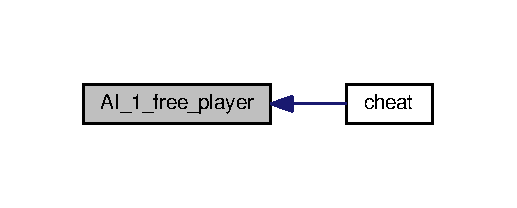
\includegraphics[width=248pt]{AI__1_8c_a064e38e8072edd14b0bef80985ddd412_icgraph}
\end{center}
\end{figure}


\hypertarget{AI__1_8c_a4b129a9daa97da56708afe7568021aa1}{\index{A\-I\-\_\-1.\-c@{A\-I\-\_\-1.\-c}!A\-I\-\_\-1\-\_\-init\-\_\-player@{A\-I\-\_\-1\-\_\-init\-\_\-player}}
\index{A\-I\-\_\-1\-\_\-init\-\_\-player@{A\-I\-\_\-1\-\_\-init\-\_\-player}!AI_1.c@{A\-I\-\_\-1.\-c}}
\subsubsection[{A\-I\-\_\-1\-\_\-init\-\_\-player}]{\setlength{\rightskip}{0pt plus 5cm}int A\-I\-\_\-1\-\_\-init\-\_\-player (
\begin{DoxyParamCaption}
\item[{int}]{id, }
\item[{int}]{nb\-\_\-players, }
\item[{int}]{nb\-\_\-towns, }
\item[{int}]{nb\-\_\-rails, }
\item[{struct {\bf Rail} $\ast$}]{rails, }
\item[{int}]{nb\-\_\-initial\-\_\-wagons, }
\item[{int}]{nb\-\_\-obj, }
\item[{struct {\bf Objective} $\ast$}]{objs}
\end{DoxyParamCaption}
)}}\label{AI__1_8c_a4b129a9daa97da56708afe7568021aa1}


A\-I\-\_\-0\-\_\-init\-\_\-player Initialises all the parameters of a struct \hyperlink{structPlayer}{Player} (composed of the general game parameters, and his own informations about the game). 


\begin{DoxyParams}{Parameters}
{\em id} & is the identifier of the player. \\
\hline
{\em nb\-\_\-players} & is the total number of players in the game. \\
\hline
{\em nb\-\_\-towns} & is the total number of towns in the game. \\
\hline
{\em nb\-\_\-rails} & is the total number of rails in the game. \\
\hline
{\em rails} & is the tabular composed of all the rails of the game. \\
\hline
{\em nb\-\_\-initial\-\_\-wagons} & is the number of wagons that each player has at the begining of the game. \\
\hline
{\em nb\-\_\-obj} & is the total number of objective-\/cards of the game. \\
\hline
{\em objs} & is the tabular composed of all the objective-\/cards of the game. \\
\hline
\end{DoxyParams}
\begin{DoxyReturn}{Returns}
Returns 1 if the initialisation went well; 0 otherwise. 
\end{DoxyReturn}


Here is the call graph for this function\-:
\nopagebreak
\begin{figure}[H]
\begin{center}
\leavevmode
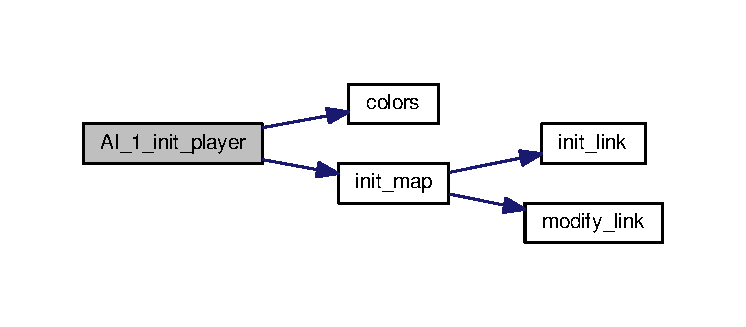
\includegraphics[width=350pt]{AI__1_8c_a4b129a9daa97da56708afe7568021aa1_cgraph}
\end{center}
\end{figure}




Here is the caller graph for this function\-:
\nopagebreak
\begin{figure}[H]
\begin{center}
\leavevmode
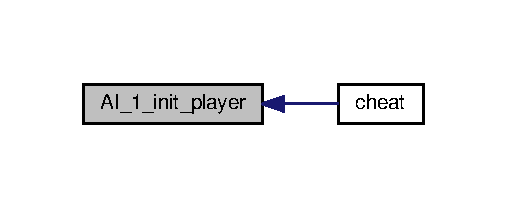
\includegraphics[width=244pt]{AI__1_8c_a4b129a9daa97da56708afe7568021aa1_icgraph}
\end{center}
\end{figure}


\hypertarget{AI__1_8c_ad92748bc33ab88fa6ea22a4da3ac71fc}{\index{A\-I\-\_\-1.\-c@{A\-I\-\_\-1.\-c}!A\-I\-\_\-1\-\_\-objective\-\_\-realised@{A\-I\-\_\-1\-\_\-objective\-\_\-realised}}
\index{A\-I\-\_\-1\-\_\-objective\-\_\-realised@{A\-I\-\_\-1\-\_\-objective\-\_\-realised}!AI_1.c@{A\-I\-\_\-1.\-c}}
\subsubsection[{A\-I\-\_\-1\-\_\-objective\-\_\-realised}]{\setlength{\rightskip}{0pt plus 5cm}int A\-I\-\_\-1\-\_\-objective\-\_\-realised (
\begin{DoxyParamCaption}
\item[{int}]{town1, }
\item[{int}]{town2, }
\item[{int}]{id}
\end{DoxyParamCaption}
)}}\label{AI__1_8c_ad92748bc33ab88fa6ea22a4da3ac71fc}


A\-I\-\_\-1\-\_\-objective\-\_\-realised. 


\begin{DoxyParams}{Parameters}
{\em town1} & is the town1 of the objective. \\
\hline
{\em town2} & is the town2 of the objective. \\
\hline
{\em id} & is the identifier of a given player. \\
\hline
\end{DoxyParams}
\begin{DoxyReturn}{Returns}
Returns 1 if the objective has been realised by the player. 
\end{DoxyReturn}


Here is the call graph for this function\-:
\nopagebreak
\begin{figure}[H]
\begin{center}
\leavevmode
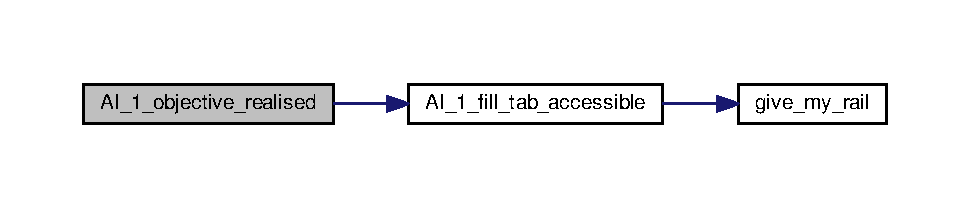
\includegraphics[width=350pt]{AI__1_8c_ad92748bc33ab88fa6ea22a4da3ac71fc_cgraph}
\end{center}
\end{figure}




Here is the caller graph for this function\-:
\nopagebreak
\begin{figure}[H]
\begin{center}
\leavevmode
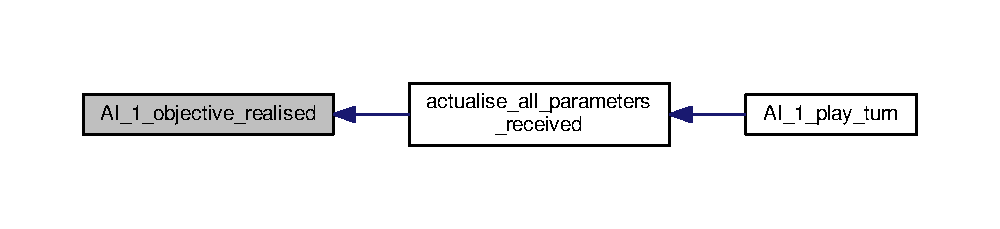
\includegraphics[width=350pt]{AI__1_8c_ad92748bc33ab88fa6ea22a4da3ac71fc_icgraph}
\end{center}
\end{figure}


\hypertarget{AI__1_8c_a8f776e760f32f938ce3203363f807f35}{\index{A\-I\-\_\-1.\-c@{A\-I\-\_\-1.\-c}!A\-I\-\_\-1\-\_\-play\-\_\-turn@{A\-I\-\_\-1\-\_\-play\-\_\-turn}}
\index{A\-I\-\_\-1\-\_\-play\-\_\-turn@{A\-I\-\_\-1\-\_\-play\-\_\-turn}!AI_1.c@{A\-I\-\_\-1.\-c}}
\subsubsection[{A\-I\-\_\-1\-\_\-play\-\_\-turn}]{\setlength{\rightskip}{0pt plus 5cm}struct {\bf Action} A\-I\-\_\-1\-\_\-play\-\_\-turn (
\begin{DoxyParamCaption}
\item[{int $\ast$}]{used\-\_\-wagons, }
\item[{int $\ast$}]{cards\-\_\-in\-\_\-hand, }
\item[{int $\ast$}]{objectives, }
\item[{int}]{nb\-\_\-new\-\_\-rails, }
\item[{struct {\bf New\-\_\-rail} $\ast$}]{changes, }
\item[{int $\ast$}]{new\-\_\-obj, }
\item[{int $\ast$}]{cards}
\end{DoxyParamCaption}
)}}\label{AI__1_8c_a8f776e760f32f938ce3203363f807f35}


A\-I\-\_\-0\-\_\-play\-\_\-turn Calls the player, actualises all the changes that occured since the last time the player was called, and asks the player which action he wants. 


\begin{DoxyParams}{Parameters}
{\em used\-\_\-wagons} & is a tabular which length is the number of players (for a given player, the tabular's value is the number of wagons he has set during the last round). \\
\hline
{\em cards\-\_\-in\-\_\-hand} & is a tabular which length is the number of players (for a given player, the tabular's value is the number of cards that the player has won or lost during the last round). \\
\hline
{\em objectives} & is a tabular composed of the number of objectives drawned by each player. \\
\hline
{\em nb\-\_\-new\-\_\-rails} & is the length of the tabular changes (= the number of rails that the current player has set during the last round). \\
\hline
{\em changes} & is the tabular of all the rails that the current player has set during the last round. \\
\hline
{\em new\-\_\-obj} & is the tabular of the objectives that the current player has drawned during the last round. \\
\hline
{\em cards} & If the action chosen in the last round was \char`\"{}draw\char`\"{}\-: \char`\"{}cards\char`\"{} is the tabuler of all the colors (= wagon-\/cards) drawned. If the action chosen was \char`\"{}build\char`\"{}\-: \char`\"{}cards\char`\"{} is the tabular of all the colors lost (because set). \\
\hline
\end{DoxyParams}
\begin{DoxyReturn}{Returns}
Returns the struct \hyperlink{structAction}{Action} chosen and completed by the player according to his strategy. 
\end{DoxyReturn}


Here is the call graph for this function\-:
\nopagebreak
\begin{figure}[H]
\begin{center}
\leavevmode
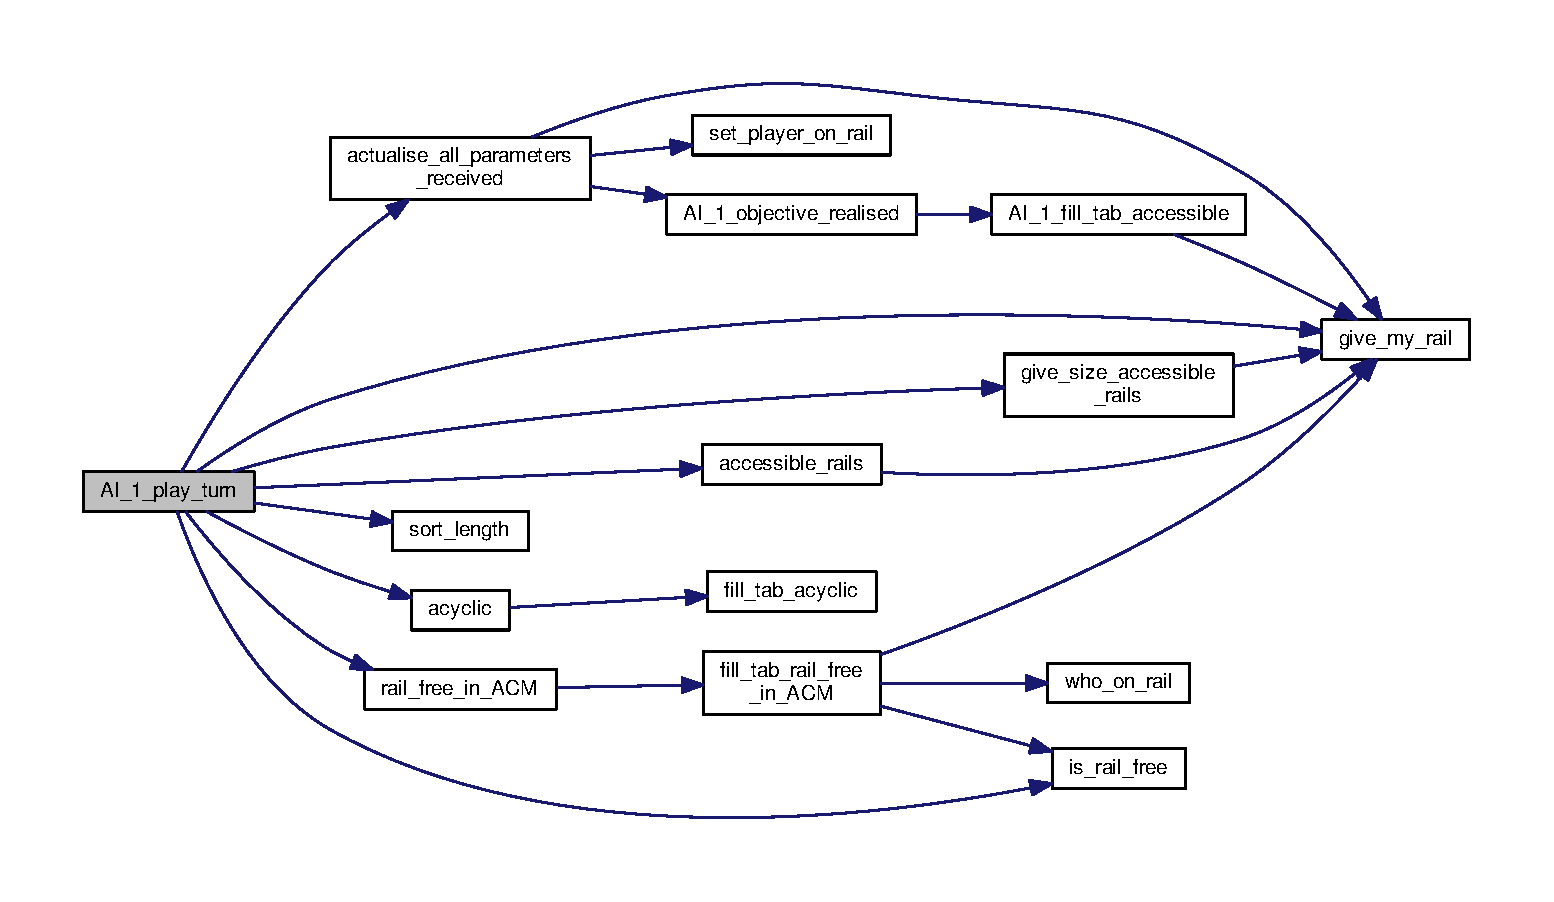
\includegraphics[width=350pt]{AI__1_8c_a8f776e760f32f938ce3203363f807f35_cgraph}
\end{center}
\end{figure}


\hypertarget{AI__1_8c_a72603999060857e266eeb57fe4651028}{\index{A\-I\-\_\-1.\-c@{A\-I\-\_\-1.\-c}!fill\-\_\-tab\-\_\-acyclic@{fill\-\_\-tab\-\_\-acyclic}}
\index{fill\-\_\-tab\-\_\-acyclic@{fill\-\_\-tab\-\_\-acyclic}!AI_1.c@{A\-I\-\_\-1.\-c}}
\subsubsection[{fill\-\_\-tab\-\_\-acyclic}]{\setlength{\rightskip}{0pt plus 5cm}void fill\-\_\-tab\-\_\-acyclic (
\begin{DoxyParamCaption}
\item[{struct {\bf Rail} $\ast$}]{tab, }
\item[{int}]{size, }
\item[{int $\ast$}]{tab\-\_\-to\-\_\-fill, }
\item[{int}]{current\-\_\-town}
\end{DoxyParamCaption}
)}}\label{AI__1_8c_a72603999060857e266eeb57fe4651028}


fill\-\_\-tab\-\_\-acyclic Is a recursive function which fills the tabular \char`\"{}tab\-\_\-to\-\_\-fill\char`\"{} (set the indice \char`\"{}i\char`\"{} at 1 if the town \char`\"{}i\char`\"{} is accessible from the town \char`\"{}current\-\_\-town\char`\"{} by using rails of the tabular \char`\"{}tab\char`\"{}, 0 otherwise). 


\begin{DoxyParams}{Parameters}
{\em tab} & is a tabular of struct Rails which is going to be analysed by the function. \\
\hline
{\em size} & is the length of the tabular \char`\"{}tab\char`\"{}. \\
\hline
{\em tab\-\_\-to\-\_\-fill} & is the tabular which is going to be filled (the indice \char`\"{}i\char`\"{} is set at 1 if the town \char`\"{}i\char`\"{} is accessible from the town \char`\"{}current\-\_\-town\char`\"{} by using rails of the tabular \char`\"{}tab\char`\"{}, 0 otherwise). \\
\hline
{\em current\-\_\-town} & is a town accessible from the first town analysed (= the first value of \char`\"{}current\-\_\-town\char`\"{}), and from which all the rails still accessible are going to be analysed. \\
\hline
\end{DoxyParams}


Here is the caller graph for this function\-:
\nopagebreak
\begin{figure}[H]
\begin{center}
\leavevmode
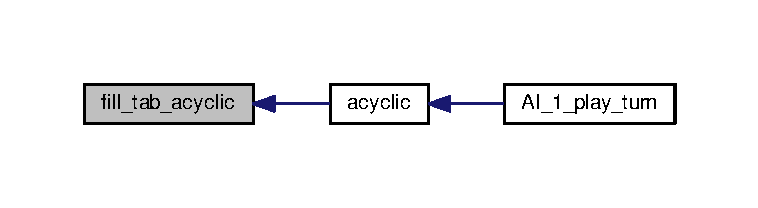
\includegraphics[width=350pt]{AI__1_8c_a72603999060857e266eeb57fe4651028_icgraph}
\end{center}
\end{figure}


\hypertarget{AI__1_8c_a570906173de0ecea152cada5a76f8a44}{\index{A\-I\-\_\-1.\-c@{A\-I\-\_\-1.\-c}!fill\-\_\-tab\-\_\-rail\-\_\-free\-\_\-in\-\_\-\-A\-C\-M@{fill\-\_\-tab\-\_\-rail\-\_\-free\-\_\-in\-\_\-\-A\-C\-M}}
\index{fill\-\_\-tab\-\_\-rail\-\_\-free\-\_\-in\-\_\-\-A\-C\-M@{fill\-\_\-tab\-\_\-rail\-\_\-free\-\_\-in\-\_\-\-A\-C\-M}!AI_1.c@{A\-I\-\_\-1.\-c}}
\subsubsection[{fill\-\_\-tab\-\_\-rail\-\_\-free\-\_\-in\-\_\-\-A\-C\-M}]{\setlength{\rightskip}{0pt plus 5cm}int fill\-\_\-tab\-\_\-rail\-\_\-free\-\_\-in\-\_\-\-A\-C\-M (
\begin{DoxyParamCaption}
\item[{struct {\bf Rail} $\ast$}]{tab, }
\item[{int $\ast$}]{acm\-\_\-tab\-\_\-indices, }
\item[{int}]{size, }
\item[{int $\ast$}]{tab\-\_\-towns\-\_\-to\-\_\-fill, }
\item[{int $\ast$}]{tab\-\_\-rails\-\_\-to\-\_\-fill, }
\item[{int}]{current\-\_\-town, }
\item[{int}]{town\-\_\-to\-\_\-reach}
\end{DoxyParamCaption}
)}}\label{AI__1_8c_a570906173de0ecea152cada5a76f8a44}


fill\-\_\-tab\-\_\-rail\-\_\-free\-\_\-in\-\_\-\-A\-C\-M 


\begin{DoxyParams}{Parameters}
{\em tab} & is the A\-C\-M tabular. \\
\hline
{\em acm\-\_\-tab\-\_\-indices} & is the tabular of the indices of the rails in \char`\"{}tab\char`\"{}. \\
\hline
{\em size} & is the length of the tabulars \char`\"{}tab\char`\"{} and \char`\"{}acm\-\_\-tab\-\_\-indices\char`\"{}. \\
\hline
{\em tab\-\_\-towns\-\_\-to\-\_\-fill} & is a boolean tab which indicates which towns are accessible by town1 or town2 of an objective. \\
\hline
{\em tab\-\_\-rails\-\_\-to\-\_\-fill} & is a boolean tab which indicates which rails are accessible by town1 or town2 of an objective. \\
\hline
{\em current\-\_\-town} & is called at the begining with town1 or town2 of an objective owned by the player; the function is going to set at 1 \char`\"{}tab\-\_\-towns\-\_\-to\-\_\-fill\mbox{[}i\mbox{]}\char`\"{} and \char`\"{}tab\-\_\-rails\-\_\-to\-\_\-fill\mbox{[}j\mbox{]}\char`\"{} if the town \char`\"{}i\char`\"{} and the rail \char`\"{}j\char`\"{} are accessible by the player from the town2. \\
\hline
\end{DoxyParams}


Here is the call graph for this function\-:
\nopagebreak
\begin{figure}[H]
\begin{center}
\leavevmode
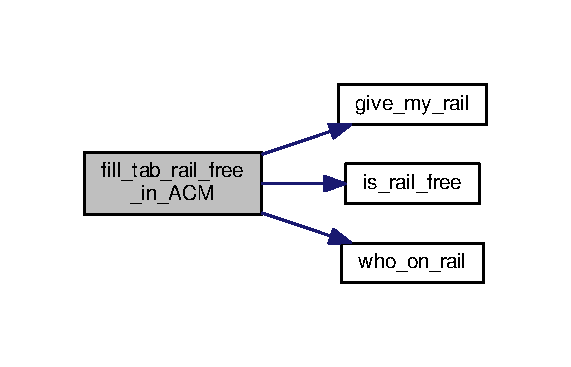
\includegraphics[width=274pt]{AI__1_8c_a570906173de0ecea152cada5a76f8a44_cgraph}
\end{center}
\end{figure}




Here is the caller graph for this function\-:
\nopagebreak
\begin{figure}[H]
\begin{center}
\leavevmode
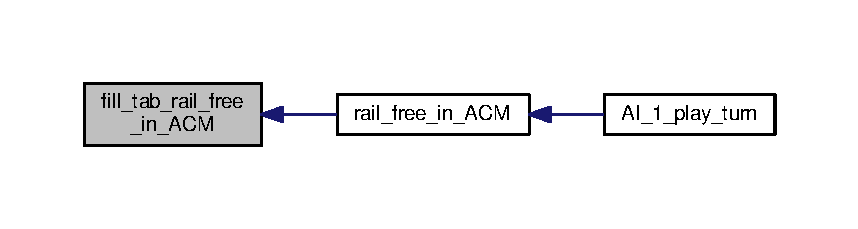
\includegraphics[width=350pt]{AI__1_8c_a570906173de0ecea152cada5a76f8a44_icgraph}
\end{center}
\end{figure}


\hypertarget{AI__1_8c_a1795878e593a98deac75d49b176d5591}{\index{A\-I\-\_\-1.\-c@{A\-I\-\_\-1.\-c}!give\-\_\-size\-\_\-accessible\-\_\-rails@{give\-\_\-size\-\_\-accessible\-\_\-rails}}
\index{give\-\_\-size\-\_\-accessible\-\_\-rails@{give\-\_\-size\-\_\-accessible\-\_\-rails}!AI_1.c@{A\-I\-\_\-1.\-c}}
\subsubsection[{give\-\_\-size\-\_\-accessible\-\_\-rails}]{\setlength{\rightskip}{0pt plus 5cm}int give\-\_\-size\-\_\-accessible\-\_\-rails (
\begin{DoxyParamCaption}
\item[{struct {\bf Rail} $\ast$}]{tab, }
\item[{int}]{size, }
\item[{int}]{id}
\end{DoxyParamCaption}
)}}\label{AI__1_8c_a1795878e593a98deac75d49b176d5591}


give\-\_\-size\-\_\-accessible\-\_\-rails 


\begin{DoxyParams}{Parameters}
{\em tab} & is the tabular of struct \hyperlink{structRail}{Rail} of which the function is going to count the non-\/occupied rails and the rails occupied by a given player. \\
\hline
{\em size} & is the size of the tabular \char`\"{}tab\char`\"{}. \\
\hline
{\em id} & is the identifier of a given player. \\
\hline
\end{DoxyParams}
\begin{DoxyReturn}{Returns}
Returns a tabular of the rails from the tabular \char`\"{}tab\char`\"{} not already occupied by other players. 
\end{DoxyReturn}


Here is the call graph for this function\-:
\nopagebreak
\begin{figure}[H]
\begin{center}
\leavevmode
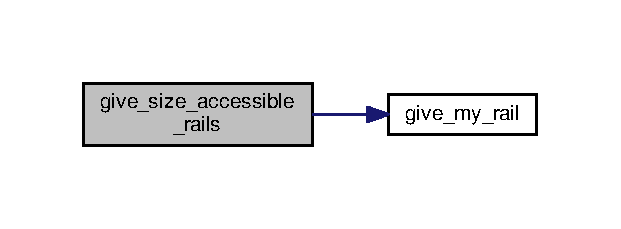
\includegraphics[width=298pt]{AI__1_8c_a1795878e593a98deac75d49b176d5591_cgraph}
\end{center}
\end{figure}




Here is the caller graph for this function\-:
\nopagebreak
\begin{figure}[H]
\begin{center}
\leavevmode
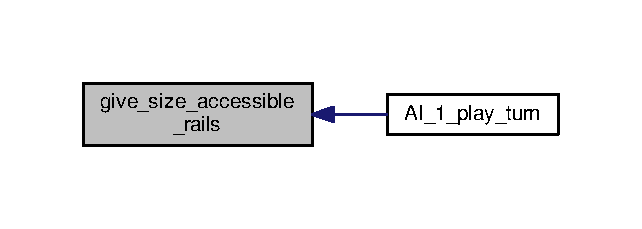
\includegraphics[width=308pt]{AI__1_8c_a1795878e593a98deac75d49b176d5591_icgraph}
\end{center}
\end{figure}


\hypertarget{AI__1_8c_aa14010606b2c569bd491a7101a020023}{\index{A\-I\-\_\-1.\-c@{A\-I\-\_\-1.\-c}!min\-\_\-point\-\_\-objs@{min\-\_\-point\-\_\-objs}}
\index{min\-\_\-point\-\_\-objs@{min\-\_\-point\-\_\-objs}!AI_1.c@{A\-I\-\_\-1.\-c}}
\subsubsection[{min\-\_\-point\-\_\-objs}]{\setlength{\rightskip}{0pt plus 5cm}int min\-\_\-point\-\_\-objs (
\begin{DoxyParamCaption}
\item[{int}]{nb, }
\item[{int $\ast$}]{objs, }
\item[{int $\ast$}]{tab}
\end{DoxyParamCaption}
)}}\label{AI__1_8c_aa14010606b2c569bd491a7101a020023}


min\-\_\-point\-\_\-objs 


\begin{DoxyParams}{Parameters}
{\em nb} & is the length of the tabular \char`\"{}objs\char`\"{}. \\
\hline
{\em objs} & is a tabular of objectives proposed to the player (it is the tabular of the indices of the objectives). \\
\hline
{\em tab} & is a tabular indicating which objectives have already been chosen (tab\mbox{[}i\mbox{]}=1 if the objective \char`\"{}i\char`\"{} has already been chosen, 0 otherwise). \\
\hline
\end{DoxyParams}
\begin{DoxyReturn}{Returns}
Returns the objective (not already chosen by the player) which has the minimal number of points in the tabular \char`\"{}objs\char`\"{}. 
\end{DoxyReturn}


Here is the caller graph for this function\-:
\nopagebreak
\begin{figure}[H]
\begin{center}
\leavevmode
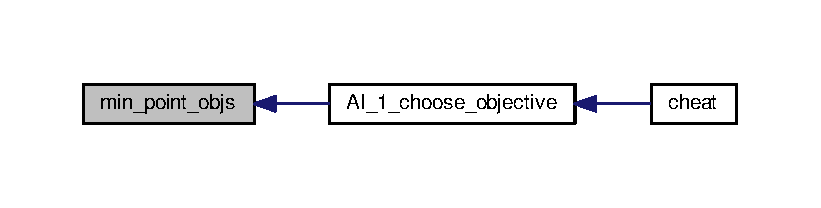
\includegraphics[width=350pt]{AI__1_8c_aa14010606b2c569bd491a7101a020023_icgraph}
\end{center}
\end{figure}


\hypertarget{AI__1_8c_ab12b4fcf8835504e67cc690b905a6e3c}{\index{A\-I\-\_\-1.\-c@{A\-I\-\_\-1.\-c}!rail\-\_\-free\-\_\-in\-\_\-\-A\-C\-M@{rail\-\_\-free\-\_\-in\-\_\-\-A\-C\-M}}
\index{rail\-\_\-free\-\_\-in\-\_\-\-A\-C\-M@{rail\-\_\-free\-\_\-in\-\_\-\-A\-C\-M}!AI_1.c@{A\-I\-\_\-1.\-c}}
\subsubsection[{rail\-\_\-free\-\_\-in\-\_\-\-A\-C\-M}]{\setlength{\rightskip}{0pt plus 5cm}int rail\-\_\-free\-\_\-in\-\_\-\-A\-C\-M (
\begin{DoxyParamCaption}
\item[{struct {\bf Rail} $\ast$}]{acm, }
\item[{int $\ast$}]{acm\-\_\-tab\-\_\-indices, }
\item[{int}]{size, }
\item[{int}]{town1, }
\item[{int}]{town2}
\end{DoxyParamCaption}
)}}\label{AI__1_8c_ab12b4fcf8835504e67cc690b905a6e3c}


rail\-\_\-free\-\_\-in\-\_\-\-A\-C\-M 


\begin{DoxyParams}{Parameters}
{\em acm} & is the tabular in which the function is going to search for a free rail between town1 and town2 if the all way between the two towns is free. \\
\hline
{\em acm\-\_\-tab\-\_\-indices} & is the tabular of the indices of the rails in the tabular \char`\"{}acm\char`\"{}. \\
\hline
{\em size} & is the length of the tabulars \char`\"{}acm\char`\"{} and \char`\"{}acm\-\_\-tab\-\_\-indices\char`\"{}. \\
\hline
{\em town1} & is the town1 of a given objective. \\
\hline
{\em town2} & is the town2 of of a given objective. \\
\hline
\end{DoxyParams}
\begin{DoxyReturn}{Returns}
Returns the indice of a free rail between the two towns of the objective given if the all way is still free or partially owned by the player and if the player has enough wagons and wagon-\/cards to build this rail; returns -\/1 otherwise. 
\end{DoxyReturn}


Here is the call graph for this function\-:
\nopagebreak
\begin{figure}[H]
\begin{center}
\leavevmode
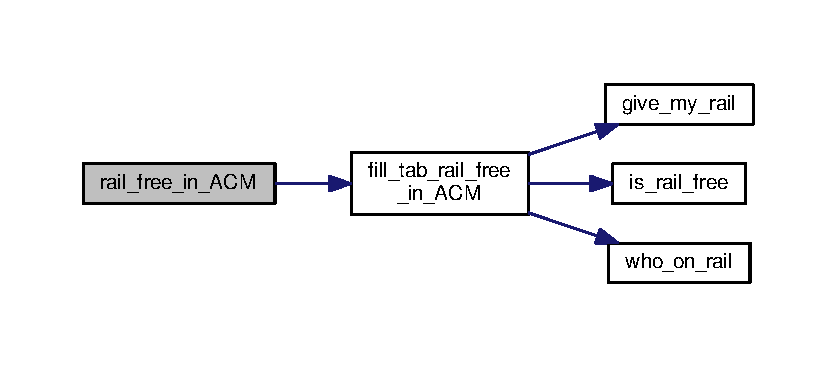
\includegraphics[width=350pt]{AI__1_8c_ab12b4fcf8835504e67cc690b905a6e3c_cgraph}
\end{center}
\end{figure}




Here is the caller graph for this function\-:
\nopagebreak
\begin{figure}[H]
\begin{center}
\leavevmode
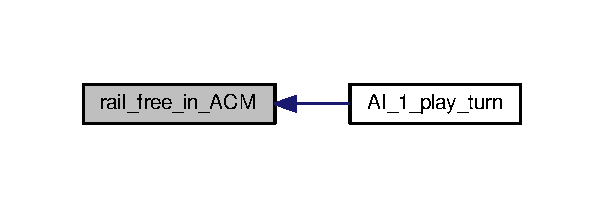
\includegraphics[width=290pt]{AI__1_8c_ab12b4fcf8835504e67cc690b905a6e3c_icgraph}
\end{center}
\end{figure}


\hypertarget{AI__1_8c_ac3468cbfd5d55ca81b2d1f65c77263c3}{\index{A\-I\-\_\-1.\-c@{A\-I\-\_\-1.\-c}!sort\-\_\-length@{sort\-\_\-length}}
\index{sort\-\_\-length@{sort\-\_\-length}!AI_1.c@{A\-I\-\_\-1.\-c}}
\subsubsection[{sort\-\_\-length}]{\setlength{\rightskip}{0pt plus 5cm}void sort\-\_\-length (
\begin{DoxyParamCaption}
\item[{struct {\bf Rail} $\ast$}]{tab, }
\item[{int $\ast$}]{tab\-\_\-indices, }
\item[{int}]{size}
\end{DoxyParamCaption}
)}}\label{AI__1_8c_ac3468cbfd5d55ca81b2d1f65c77263c3}


sort\-\_\-length 


\begin{DoxyParams}{Parameters}
{\em tab} & is the tabular of struc Rails which is going to be sorted by the function (from the shortest rail to the longest). \\
\hline
{\em tab\-\_\-indices} & is the tabular of indices of rails which is going to be sorted (from the shortest rail to the longest). \\
\hline
{\em size} & is the size of the tabulars \char`\"{}tab\char`\"{} and \char`\"{}tab\-\_\-indices\char`\"{}. \\
\hline
\end{DoxyParams}


Here is the caller graph for this function\-:
\nopagebreak
\begin{figure}[H]
\begin{center}
\leavevmode
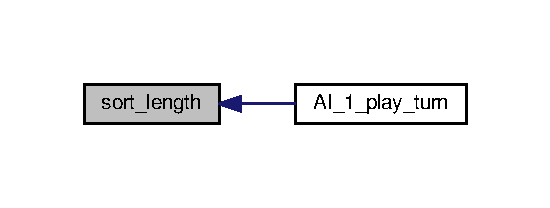
\includegraphics[width=264pt]{AI__1_8c_ac3468cbfd5d55ca81b2d1f65c77263c3_icgraph}
\end{center}
\end{figure}




\subsection{Variable Documentation}
\hypertarget{AI__1_8c_a47a2d030ed3cc6ecfbb6afd9a65b7869}{\index{A\-I\-\_\-1.\-c@{A\-I\-\_\-1.\-c}!A\-I\-\_\-1@{A\-I\-\_\-1}}
\index{A\-I\-\_\-1@{A\-I\-\_\-1}!AI_1.c@{A\-I\-\_\-1.\-c}}
\subsubsection[{A\-I\-\_\-1}]{\setlength{\rightskip}{0pt plus 5cm}struct {\bf Player} A\-I\-\_\-1}}\label{AI__1_8c_a47a2d030ed3cc6ecfbb6afd9a65b7869}

\hypertarget{build__rail_8c}{\section{/net/malt/i/sbrouard/\-Documents/projets6/s6-\/rails-\/1992/trunk/src/build\-\_\-rail.c File Reference}
\label{build__rail_8c}\index{/net/malt/i/sbrouard/\-Documents/projets6/s6-\/rails-\/1992/trunk/src/build\-\_\-rail.\-c@{/net/malt/i/sbrouard/\-Documents/projets6/s6-\/rails-\/1992/trunk/src/build\-\_\-rail.\-c}}
}
{\ttfamily \#include $<$stdio.\-h$>$}\\*
{\ttfamily \#include $<$stdlib.\-h$>$}\\*
{\ttfamily \#include \char`\"{}interface.\-h\char`\"{}}\\*
{\ttfamily \#include \char`\"{}server.\-h\char`\"{}}\\*
Include dependency graph for build\-\_\-rail.\-c\-:
\nopagebreak
\begin{figure}[H]
\begin{center}
\leavevmode
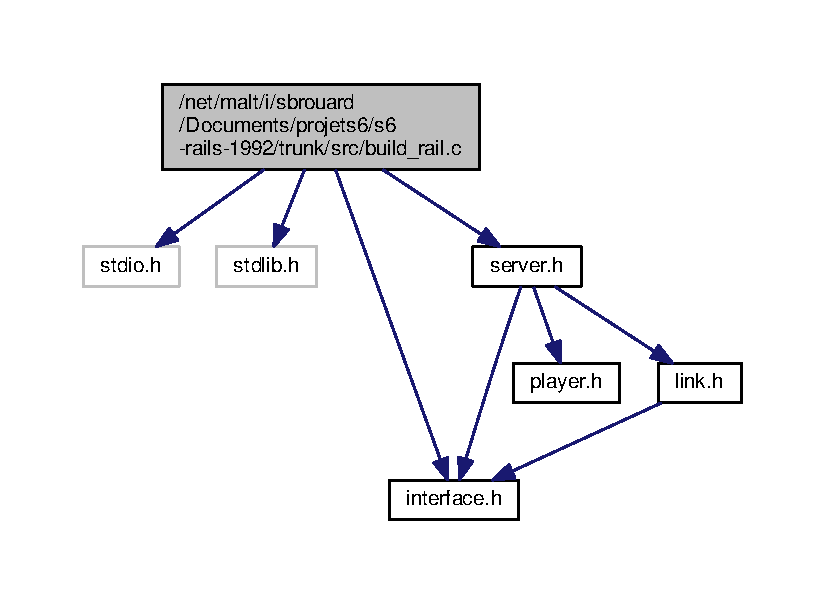
\includegraphics[width=350pt]{build__rail_8c__incl}
\end{center}
\end{figure}
\subsection*{Functions}
\begin{DoxyCompactItemize}
\item 
void \hyperlink{build__rail_8c_ada2781c3fc6ea007f3426d76fbcb8082}{build\-\_\-rail} (int player, int nb\-\_\-players, int rail, int $\ast$$\ast$card\-\_\-hands, int $\ast$nb\-\_\-cards, int $\ast$wagon\-\_\-cards\-\_\-modif, int $\ast$$\ast$cards, struct \hyperlink{structLink}{Link} $\ast$$\ast$map, struct \hyperlink{structRail}{Rail} $\ast$rails, int $\ast$wagons\-\_\-remaining, int $\ast$used\-\_\-wagons)
\begin{DoxyCompactList}\small\item\em build\-\_\-rail Applies modification in the map and the player when a player builds a rail \end{DoxyCompactList}\end{DoxyCompactItemize}


\subsection{Function Documentation}
\hypertarget{build__rail_8c_ada2781c3fc6ea007f3426d76fbcb8082}{\index{build\-\_\-rail.\-c@{build\-\_\-rail.\-c}!build\-\_\-rail@{build\-\_\-rail}}
\index{build\-\_\-rail@{build\-\_\-rail}!build_rail.c@{build\-\_\-rail.\-c}}
\subsubsection[{build\-\_\-rail}]{\setlength{\rightskip}{0pt plus 5cm}void build\-\_\-rail (
\begin{DoxyParamCaption}
\item[{int}]{player, }
\item[{int}]{nb\-\_\-players, }
\item[{int}]{rail, }
\item[{int $\ast$$\ast$}]{card\-\_\-hand, }
\item[{int $\ast$}]{nb\-\_\-cards, }
\item[{int $\ast$}]{wagon\-\_\-cards\-\_\-modif, }
\item[{int $\ast$$\ast$}]{cards, }
\item[{struct {\bf Link} $\ast$$\ast$}]{map, }
\item[{struct {\bf Rail} $\ast$}]{rails, }
\item[{int $\ast$}]{wagons\-\_\-remaining, }
\item[{int $\ast$}]{used\-\_\-wagons}
\end{DoxyParamCaption}
)}}\label{build__rail_8c_ada2781c3fc6ea007f3426d76fbcb8082}


build\-\_\-rail Applies modification in the map and the player when a player builds a rail 


\begin{DoxyParams}{Parameters}
{\em player} & id of the player who is playing \\
\hline
{\em nb\-\_\-players} & total number of player in the game \\
\hline
{\em rail} & id of the rail that the player want to build \\
\hline
{\em card\-\_\-hand} & colors of cards of each player \\
\hline
{\em nb\-\_\-cards} & array of number of color cards of each player \\
\hline
{\em wagon\-\_\-cards\-\_\-modif} & array of number of more (+) or less (-\/) cards of each player \\
\hline
{\em cards} & array of colors of changed cards of each player \\
\hline
{\em map} & \\
\hline
{\em rails} & Array with all the rails \\
\hline
{\em nb\-\_\-rails} & \\
\hline
{\em wagons\-\_\-remaining} & array of number of wagons remaining for each player \\
\hline
{\em used\-\_\-wagons} & array of number of wagons used during this turn \\
\hline
\end{DoxyParams}


Here is the caller graph for this function\-:
\nopagebreak
\begin{figure}[H]
\begin{center}
\leavevmode
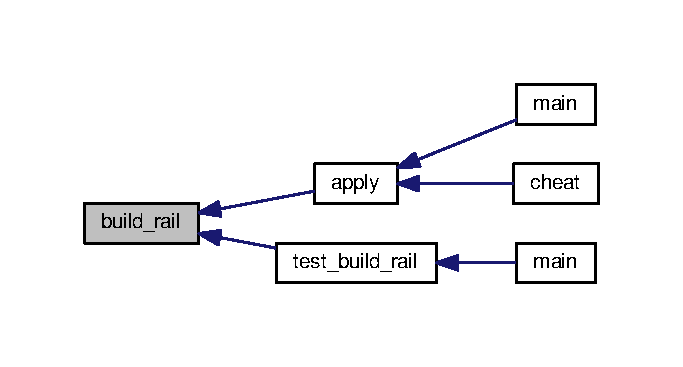
\includegraphics[width=328pt]{build__rail_8c_ada2781c3fc6ea007f3426d76fbcb8082_icgraph}
\end{center}
\end{figure}



\hypertarget{cards__gestion_8c}{\section{/net/malt/i/sbrouard/\-Documents/projets6/s6-\/rails-\/1992/trunk/src/cards\-\_\-gestion.c File Reference}
\label{cards__gestion_8c}\index{/net/malt/i/sbrouard/\-Documents/projets6/s6-\/rails-\/1992/trunk/src/cards\-\_\-gestion.\-c@{/net/malt/i/sbrouard/\-Documents/projets6/s6-\/rails-\/1992/trunk/src/cards\-\_\-gestion.\-c}}
}
{\ttfamily \#include $<$stdio.\-h$>$}\\*
{\ttfamily \#include $<$stdlib.\-h$>$}\\*
{\ttfamily \#include \char`\"{}interface.\-h\char`\"{}}\\*
{\ttfamily \#include \char`\"{}server.\-h\char`\"{}}\\*
{\ttfamily \#include \char`\"{}link.\-h\char`\"{}}\\*
{\ttfamily \#include \char`\"{}concat.\-h\char`\"{}}\\*
{\ttfamily \#include $<$time.\-h$>$}\\*
Include dependency graph for cards\-\_\-gestion.\-c\-:
\nopagebreak
\begin{figure}[H]
\begin{center}
\leavevmode
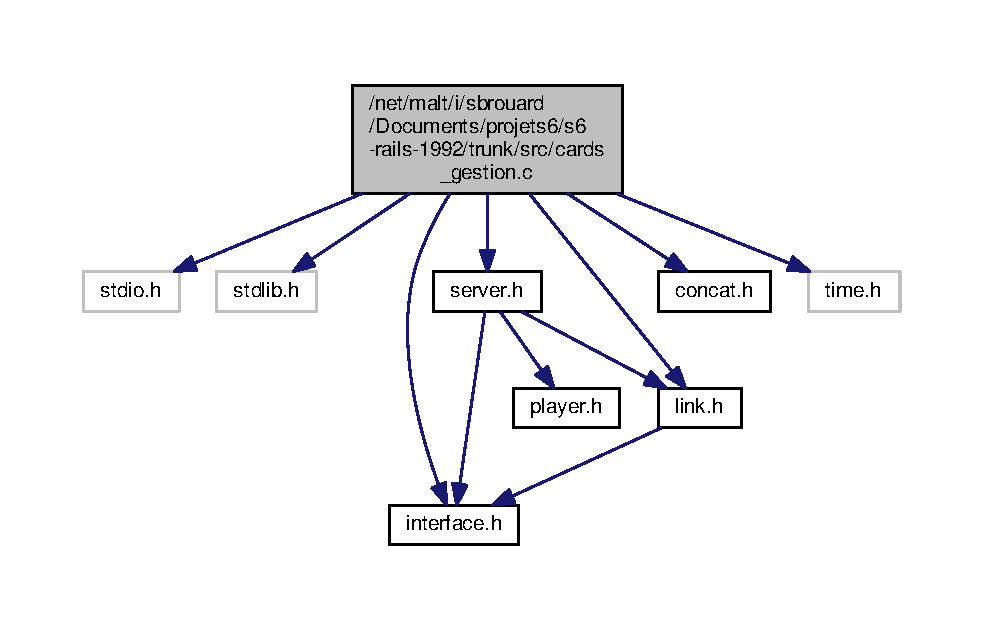
\includegraphics[width=350pt]{cards__gestion_8c__incl}
\end{center}
\end{figure}
\subsection*{Functions}
\begin{DoxyCompactItemize}
\item 
int \hyperlink{cards__gestion_8c_a6476a83be99f343b2baff69567b03280}{colors} (struct \hyperlink{structRail}{Rail} $\ast$rails, int nb\-\_\-rails, int $\ast$$\ast$col)
\begin{DoxyCompactList}\small\item\em colors Complete the array with the colors used in the game and return the number of colors \end{DoxyCompactList}\item 
void \hyperlink{cards__gestion_8c_a10839b86959ad4336606d439d85cf2ac}{init\-\_\-card\-\_\-hands} (int nb\-\_\-players, int nb\-\_\-starting\-\_\-cards, int $\ast$$\ast$card\-\_\-hands, int $\ast$\hyperlink{server_8h_a6476a83be99f343b2baff69567b03280}{colors}, int nb\-\_\-colors)
\begin{DoxyCompactList}\small\item\em init\-\_\-card\-\_\-hands initialisation of the cards in possession of each player at the beginning of the game \end{DoxyCompactList}\item 
void \hyperlink{cards__gestion_8c_abbbcd18606eb6dc90250f2d7814c17a8}{init\-\_\-obj\-\_\-hands} (int nb\-\_\-players, int nb\-\_\-starting\-\_\-objs, int $\ast$$\ast$obj\-\_\-hands, struct \hyperlink{structObjective}{Objective} $\ast$objectives, int nb\-\_\-objs, int $\ast$objectives\-\_\-condition)
\begin{DoxyCompactList}\small\item\em init\-\_\-obj\-\_\-hands \end{DoxyCompactList}\item 
void \hyperlink{cards__gestion_8c_a87f6a92801d41d1ea98ee373cb4932b8}{init\-\_\-nb\-\_\-objs} (int nb\-\_\-players, int nb\-\_\-starting\-\_\-objs, int $\ast$nb\-\_\-objs)
\begin{DoxyCompactList}\small\item\em init\-\_\-nb\-\_\-objs \end{DoxyCompactList}\item 
void \hyperlink{cards__gestion_8c_a29db272fe208ef85ffd21981b50dbe23}{draw\-\_\-color\-\_\-card} (int player, int nb\-\_\-players, int $\ast$$\ast$card\-\_\-hand, int $\ast$nb\-\_\-cards, int $\ast$wagon\-\_\-cards\-\_\-modif, int $\ast$$\ast$cards, int nb\-\_\-colors, int $\ast$\hyperlink{server_8h_a6476a83be99f343b2baff69567b03280}{colors}, int colored\-\_\-game)
\begin{DoxyCompactList}\small\item\em draw\-\_\-color\-\_\-card applies modif if the player draw color cards \end{DoxyCompactList}\item 
void \hyperlink{cards__gestion_8c_a87da09cde6e4fc0c6d8d8280bd4863d9}{draw\-\_\-objectives} (int player, int nb\-\_\-players, int $\ast$$\ast$obj\-\_\-hands, int nb\-\_\-objs\-\_\-total, int $\ast$objs\-\_\-cond, int $\ast$$\ast$new\-\_\-objs, int nb\-\_\-objs\-\_\-drawn\-\_\-max, int min\-\_\-objs\-\_\-to\-\_\-pick, struct \hyperlink{structf__player}{f\-\_\-player} $\ast$player\-\_\-fonctions, int $\ast$nb\-\_\-objs, int $\ast$nb\-\_\-new\-\_\-objs)
\begin{DoxyCompactList}\small\item\em draw\-\_\-objectives Applies modification in the server and the player when a player draws objectives \end{DoxyCompactList}\item 
void \hyperlink{cards__gestion_8c_a720d4a54fde8ac30d82ea055669dfc6c}{init\-\_\-first\-\_\-chosen\-\_\-objs} (int $\ast$T\-\_\-chosen\-\_\-objs, int nb\-\_\-objs\-\_\-given, int $\ast$all\-\_\-objective\-\_\-conditions, int all\-\_\-objs\-\_\-conditions\-\_\-size, int $\ast$obj\-\_\-player\-\_\-hand, int $\ast$nb\-\_\-objs, int $\ast$objectives, int $\ast$new\-\_\-obj, int player)
\begin{DoxyCompactList}\small\item\em init\-\_\-first\-\_\-chosen\-\_\-objs modifies the initial hand of objectives of a player, the informations about objectives in function of his choice \end{DoxyCompactList}\end{DoxyCompactItemize}


\subsection{Function Documentation}
\hypertarget{cards__gestion_8c_a6476a83be99f343b2baff69567b03280}{\index{cards\-\_\-gestion.\-c@{cards\-\_\-gestion.\-c}!colors@{colors}}
\index{colors@{colors}!cards_gestion.c@{cards\-\_\-gestion.\-c}}
\subsubsection[{colors}]{\setlength{\rightskip}{0pt plus 5cm}int colors (
\begin{DoxyParamCaption}
\item[{struct {\bf Rail} $\ast$}]{rails, }
\item[{int}]{nb\-\_\-rails, }
\item[{int $\ast$$\ast$}]{col}
\end{DoxyParamCaption}
)}}\label{cards__gestion_8c_a6476a83be99f343b2baff69567b03280}


colors Complete the array with the colors used in the game and return the number of colors 


\begin{DoxyParams}{Parameters}
{\em rails} & Array with all the rails, where there are the colors \\
\hline
{\em nb\-\_\-rails} & The number of rails, length of rails \\
\hline
{\em col} & Array to be completed \\
\hline
\end{DoxyParams}
\begin{DoxyReturn}{Returns}
The number of colors in the game = length of colors 
\end{DoxyReturn}


Here is the caller graph for this function\-:
\nopagebreak
\begin{figure}[H]
\begin{center}
\leavevmode
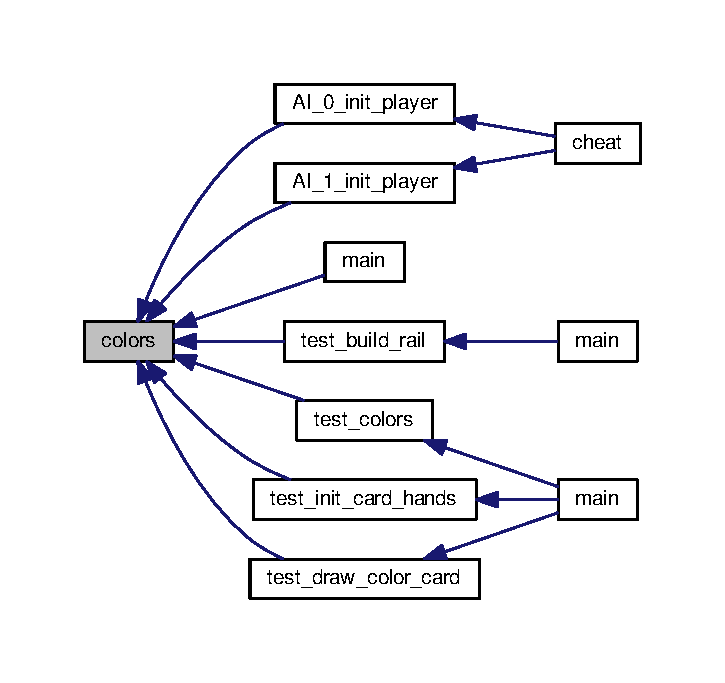
\includegraphics[width=348pt]{cards__gestion_8c_a6476a83be99f343b2baff69567b03280_icgraph}
\end{center}
\end{figure}


\hypertarget{cards__gestion_8c_a29db272fe208ef85ffd21981b50dbe23}{\index{cards\-\_\-gestion.\-c@{cards\-\_\-gestion.\-c}!draw\-\_\-color\-\_\-card@{draw\-\_\-color\-\_\-card}}
\index{draw\-\_\-color\-\_\-card@{draw\-\_\-color\-\_\-card}!cards_gestion.c@{cards\-\_\-gestion.\-c}}
\subsubsection[{draw\-\_\-color\-\_\-card}]{\setlength{\rightskip}{0pt plus 5cm}void draw\-\_\-color\-\_\-card (
\begin{DoxyParamCaption}
\item[{int}]{player, }
\item[{int}]{nb\-\_\-players, }
\item[{int $\ast$$\ast$}]{card\-\_\-hand, }
\item[{int $\ast$}]{nb\-\_\-cards, }
\item[{int $\ast$}]{wagon\-\_\-cards\-\_\-modif, }
\item[{int $\ast$$\ast$}]{cards, }
\item[{int}]{nb\-\_\-colors, }
\item[{int $\ast$}]{col, }
\item[{int}]{colored\-\_\-game}
\end{DoxyParamCaption}
)}}\label{cards__gestion_8c_a29db272fe208ef85ffd21981b50dbe23}


draw\-\_\-color\-\_\-card applies modif if the player draw color cards 


\begin{DoxyParams}{Parameters}
{\em player} & player who is playing \\
\hline
{\em nb\-\_\-players} & \\
\hline
{\em card\-\_\-hand} & colors of cards of each player \\
\hline
{\em nb\-\_\-cards} & array of number of color cards of each player \\
\hline
{\em wagon\-\_\-cards\-\_\-modif} & array of number of more (+) or less (-\/) cards of each player \\
\hline
{\em cards} & array of colors of changed cards of each player \\
\hline
{\em nb\-\_\-colors} & nb of different colors in the game \\
\hline
{\em col} & array of all the colors in the game \\
\hline
\end{DoxyParams}


Here is the caller graph for this function\-:
\nopagebreak
\begin{figure}[H]
\begin{center}
\leavevmode
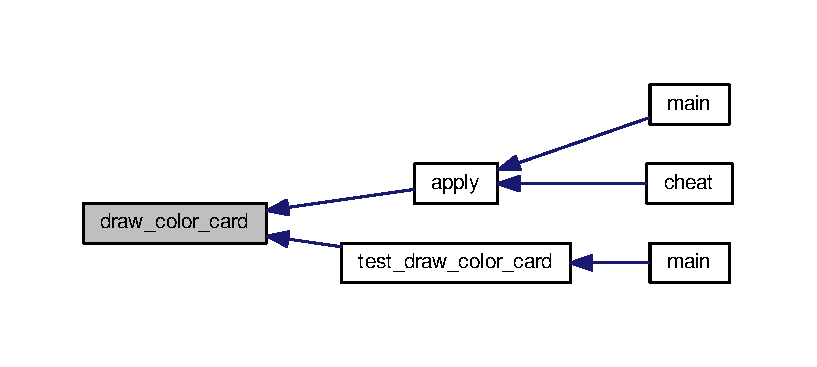
\includegraphics[width=350pt]{cards__gestion_8c_a29db272fe208ef85ffd21981b50dbe23_icgraph}
\end{center}
\end{figure}


\hypertarget{cards__gestion_8c_a87da09cde6e4fc0c6d8d8280bd4863d9}{\index{cards\-\_\-gestion.\-c@{cards\-\_\-gestion.\-c}!draw\-\_\-objectives@{draw\-\_\-objectives}}
\index{draw\-\_\-objectives@{draw\-\_\-objectives}!cards_gestion.c@{cards\-\_\-gestion.\-c}}
\subsubsection[{draw\-\_\-objectives}]{\setlength{\rightskip}{0pt plus 5cm}void draw\-\_\-objectives (
\begin{DoxyParamCaption}
\item[{int}]{player, }
\item[{int}]{nb\-\_\-players, }
\item[{int $\ast$$\ast$}]{obj\-\_\-hands, }
\item[{int}]{nb\-\_\-objs\-\_\-total, }
\item[{int $\ast$}]{objs\-\_\-cond, }
\item[{int $\ast$$\ast$}]{new\-\_\-objs, }
\item[{int}]{nb\-\_\-objs\-\_\-drawn\-\_\-max, }
\item[{int}]{min\-\_\-objs\-\_\-to\-\_\-pick, }
\item[{struct {\bf f\-\_\-player} $\ast$}]{player\-\_\-fonctions, }
\item[{int $\ast$}]{nb\-\_\-objs, }
\item[{int $\ast$}]{nb\-\_\-new\-\_\-objs}
\end{DoxyParamCaption}
)}}\label{cards__gestion_8c_a87da09cde6e4fc0c6d8d8280bd4863d9}


draw\-\_\-objectives Applies modification in the server and the player when a player draws objectives 


\begin{DoxyParams}{Parameters}
{\em player} & id of the player who is playing \\
\hline
{\em nb\-\_\-players} & \\
\hline
{\em obj\-\_\-hands} & matrix whith all objs of each player \\
\hline
{\em nb\-\_\-objs\-\_\-total} & number of total objectives in the game \\
\hline
{\em objs\-\_\-cond} & array of boleans 1=player draws this onjective, 0=he doesn't \\
\hline
{\em new\-\_\-objs} & array of new objs for each player \\
\hline
{\em nb\-\_\-objs\-\_\-drawn\-\_\-max} & \\
\hline
\end{DoxyParams}


Here is the call graph for this function\-:
\nopagebreak
\begin{figure}[H]
\begin{center}
\leavevmode
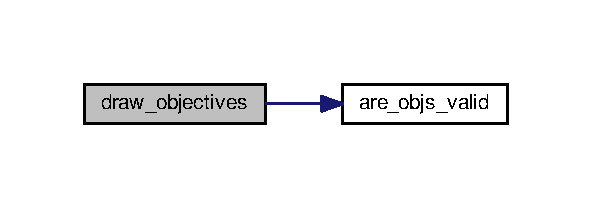
\includegraphics[width=284pt]{cards__gestion_8c_a87da09cde6e4fc0c6d8d8280bd4863d9_cgraph}
\end{center}
\end{figure}




Here is the caller graph for this function\-:
\nopagebreak
\begin{figure}[H]
\begin{center}
\leavevmode
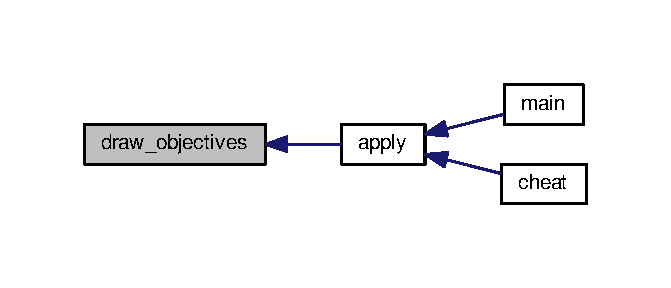
\includegraphics[width=322pt]{cards__gestion_8c_a87da09cde6e4fc0c6d8d8280bd4863d9_icgraph}
\end{center}
\end{figure}


\hypertarget{cards__gestion_8c_a10839b86959ad4336606d439d85cf2ac}{\index{cards\-\_\-gestion.\-c@{cards\-\_\-gestion.\-c}!init\-\_\-card\-\_\-hands@{init\-\_\-card\-\_\-hands}}
\index{init\-\_\-card\-\_\-hands@{init\-\_\-card\-\_\-hands}!cards_gestion.c@{cards\-\_\-gestion.\-c}}
\subsubsection[{init\-\_\-card\-\_\-hands}]{\setlength{\rightskip}{0pt plus 5cm}void init\-\_\-card\-\_\-hands (
\begin{DoxyParamCaption}
\item[{int}]{nb\-\_\-players, }
\item[{int}]{nb\-\_\-starting\-\_\-objs, }
\item[{int $\ast$$\ast$}]{card\-\_\-hands, }
\item[{int $\ast$}]{colors, }
\item[{int}]{nb\-\_\-colors}
\end{DoxyParamCaption}
)}}\label{cards__gestion_8c_a10839b86959ad4336606d439d85cf2ac}


init\-\_\-card\-\_\-hands initialisation of the cards in possession of each player at the beginning of the game 


\begin{DoxyParams}{Parameters}
{\em card\-\_\-hands} & array to be completed \\
\hline
{\em colors} & array of all colors \\
\hline
{\em nb\-\_\-colors} & nomber of colors = length of color \\
\hline
\end{DoxyParams}


Here is the caller graph for this function\-:
\nopagebreak
\begin{figure}[H]
\begin{center}
\leavevmode
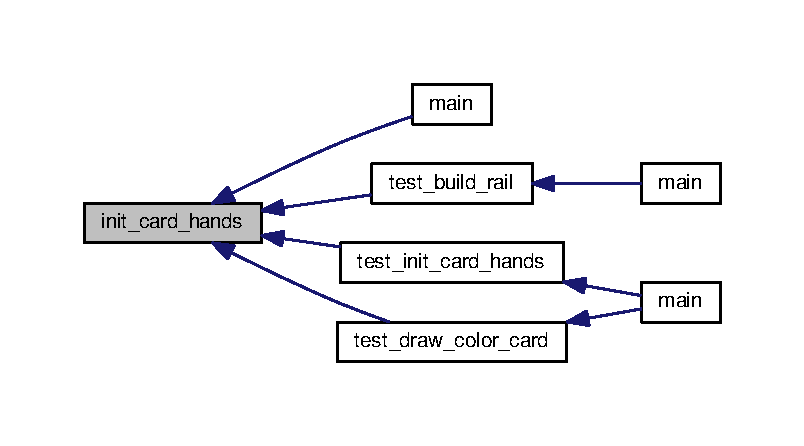
\includegraphics[width=350pt]{cards__gestion_8c_a10839b86959ad4336606d439d85cf2ac_icgraph}
\end{center}
\end{figure}


\hypertarget{cards__gestion_8c_a720d4a54fde8ac30d82ea055669dfc6c}{\index{cards\-\_\-gestion.\-c@{cards\-\_\-gestion.\-c}!init\-\_\-first\-\_\-chosen\-\_\-objs@{init\-\_\-first\-\_\-chosen\-\_\-objs}}
\index{init\-\_\-first\-\_\-chosen\-\_\-objs@{init\-\_\-first\-\_\-chosen\-\_\-objs}!cards_gestion.c@{cards\-\_\-gestion.\-c}}
\subsubsection[{init\-\_\-first\-\_\-chosen\-\_\-objs}]{\setlength{\rightskip}{0pt plus 5cm}void init\-\_\-first\-\_\-chosen\-\_\-objs (
\begin{DoxyParamCaption}
\item[{int $\ast$}]{T\-\_\-chosen\-\_\-objs, }
\item[{int}]{nb\-\_\-objs\-\_\-given, }
\item[{int $\ast$}]{all\-\_\-objective\-\_\-conditions, }
\item[{int}]{all\-\_\-objs\-\_\-conditions\-\_\-size, }
\item[{int $\ast$}]{obj\-\_\-player\-\_\-hand, }
\item[{int $\ast$}]{nb\-\_\-objs, }
\item[{int $\ast$}]{objectives, }
\item[{int $\ast$}]{new\-\_\-obj, }
\item[{int}]{player}
\end{DoxyParamCaption}
)}}\label{cards__gestion_8c_a720d4a54fde8ac30d82ea055669dfc6c}


init\-\_\-first\-\_\-chosen\-\_\-objs modifies the initial hand of objectives of a player, the informations about objectives in function of his choice 


\begin{DoxyParams}{Parameters}
{\em T\-\_\-chosen\-\_\-objs} & array of boolean representing the choice of the player for each objective (picked or not) \\
\hline
{\em nb\-\_\-objs\-\_\-given} & the number of objectives initially given to the player \\
\hline
{\em all\-\_\-objective\-\_\-conditions} & array of the objective conditions (1 \-: drawn and 0 \-: not) \\
\hline
{\em all\-\_\-objs\-\_\-size} & size of the array all\-\_\-objective\-\_\-conditions \\
\hline
{\em obj\-\_\-player\-\_\-hand} & array of the index of the objectives the player has \\
\hline
{\em nb\-\_\-\-\_\-player\-\_\-objs} & array the number of objectives of each player \\
\hline
{\em objectives} & array of the number of objectives drawn last turn by each player \\
\hline
{\em new\-\_\-obj} & array of the index of the objectives drawn last turn by the player \\
\hline
{\em player} & the number of the player \\
\hline
\end{DoxyParams}


Here is the caller graph for this function\-:
\nopagebreak
\begin{figure}[H]
\begin{center}
\leavevmode
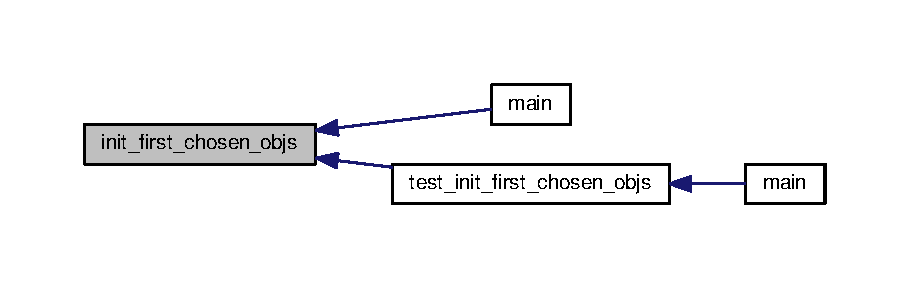
\includegraphics[width=350pt]{cards__gestion_8c_a720d4a54fde8ac30d82ea055669dfc6c_icgraph}
\end{center}
\end{figure}


\hypertarget{cards__gestion_8c_a87f6a92801d41d1ea98ee373cb4932b8}{\index{cards\-\_\-gestion.\-c@{cards\-\_\-gestion.\-c}!init\-\_\-nb\-\_\-objs@{init\-\_\-nb\-\_\-objs}}
\index{init\-\_\-nb\-\_\-objs@{init\-\_\-nb\-\_\-objs}!cards_gestion.c@{cards\-\_\-gestion.\-c}}
\subsubsection[{init\-\_\-nb\-\_\-objs}]{\setlength{\rightskip}{0pt plus 5cm}void init\-\_\-nb\-\_\-objs (
\begin{DoxyParamCaption}
\item[{int}]{nb\-\_\-players, }
\item[{int}]{nb\-\_\-starting\-\_\-objs, }
\item[{int $\ast$}]{nb\-\_\-objs}
\end{DoxyParamCaption}
)}}\label{cards__gestion_8c_a87f6a92801d41d1ea98ee373cb4932b8}


init\-\_\-nb\-\_\-objs 


\begin{DoxyParams}{Parameters}
{\em nb\-\_\-players} & \\
\hline
{\em nb\-\_\-starting\-\_\-objs} & \\
\hline
{\em nb\-\_\-objs} & array with nb\-\_\-players cases which correspond to the nb of objs of each player \\
\hline
\end{DoxyParams}


Here is the caller graph for this function\-:
\nopagebreak
\begin{figure}[H]
\begin{center}
\leavevmode
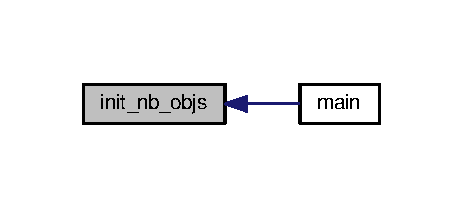
\includegraphics[width=222pt]{cards__gestion_8c_a87f6a92801d41d1ea98ee373cb4932b8_icgraph}
\end{center}
\end{figure}


\hypertarget{cards__gestion_8c_abbbcd18606eb6dc90250f2d7814c17a8}{\index{cards\-\_\-gestion.\-c@{cards\-\_\-gestion.\-c}!init\-\_\-obj\-\_\-hands@{init\-\_\-obj\-\_\-hands}}
\index{init\-\_\-obj\-\_\-hands@{init\-\_\-obj\-\_\-hands}!cards_gestion.c@{cards\-\_\-gestion.\-c}}
\subsubsection[{init\-\_\-obj\-\_\-hands}]{\setlength{\rightskip}{0pt plus 5cm}void init\-\_\-obj\-\_\-hands (
\begin{DoxyParamCaption}
\item[{int}]{nb\-\_\-players, }
\item[{int}]{nb\-\_\-starting\-\_\-objs, }
\item[{int $\ast$$\ast$}]{obj\-\_\-hands, }
\item[{struct {\bf Objective} $\ast$}]{all\-\_\-objectives, }
\item[{int}]{nb\-\_\-objs, }
\item[{int $\ast$}]{all\-\_\-objective\-\_\-conditions}
\end{DoxyParamCaption}
)}}\label{cards__gestion_8c_abbbcd18606eb6dc90250f2d7814c17a8}


init\-\_\-obj\-\_\-hands 


\begin{DoxyParams}{Parameters}
{\em nb\-\_\-players} & number of players toatal in the game \\
\hline
{\em nb\-\_\-starting\-\_\-objs} & number of objectives in the hand of each player in the beginning of the game \\
\hline
{\em obj\-\_\-hands} & array to be completed, each case is an array for each player of size nb\-\_\-starting objs, the int is the index in the array objectives \\
\hline
{\em all\-\_\-objectives} & array of all the objectives of the game \\
\hline
{\em nb\-\_\-objs} & number total of objectives in the game \\
\hline
{\em all\-\_\-objectives\-\_\-conditions} & array of booleans \-: 0 = free 1 = already drawn \\
\hline
\end{DoxyParams}


Here is the caller graph for this function\-:
\nopagebreak
\begin{figure}[H]
\begin{center}
\leavevmode
\includegraphics[width=298pt]{cards__gestion_8c_abbbcd18606eb6dc90250f2d7814c17a8_icgraph}
\end{center}
\end{figure}



\hypertarget{concat_8h}{\section{/net/malt/i/sbrouard/\-Documents/projets6/s6-\/rails-\/1992/trunk/src/concat.h File Reference}
\label{concat_8h}\index{/net/malt/i/sbrouard/\-Documents/projets6/s6-\/rails-\/1992/trunk/src/concat.\-h@{/net/malt/i/sbrouard/\-Documents/projets6/s6-\/rails-\/1992/trunk/src/concat.\-h}}
}
This graph shows which files directly or indirectly include this file\-:
\nopagebreak
\begin{figure}[H]
\begin{center}
\leavevmode
\includegraphics[width=350pt]{concat_8h__dep__incl}
\end{center}
\end{figure}
\subsection*{Macros}
\begin{DoxyCompactItemize}
\item 
\#define \hyperlink{concat_8h_ac1bd762df6f68795cfe6a980728bf233}{C\-O\-N\-C\-A\-T1}(a, b)~a \#\# b
\item 
\#define \hyperlink{concat_8h_a88fa737059e67b4b17ec980e5877361e}{C\-O\-N\-C\-A\-T}(a, b)~\hyperlink{concat_8h_ac1bd762df6f68795cfe6a980728bf233}{C\-O\-N\-C\-A\-T1}(a,b)
\end{DoxyCompactItemize}


\subsection{Macro Definition Documentation}
\hypertarget{concat_8h_a88fa737059e67b4b17ec980e5877361e}{\index{concat.\-h@{concat.\-h}!C\-O\-N\-C\-A\-T@{C\-O\-N\-C\-A\-T}}
\index{C\-O\-N\-C\-A\-T@{C\-O\-N\-C\-A\-T}!concat.h@{concat.\-h}}
\subsubsection[{C\-O\-N\-C\-A\-T}]{\setlength{\rightskip}{0pt plus 5cm}\#define C\-O\-N\-C\-A\-T(
\begin{DoxyParamCaption}
\item[{}]{a, }
\item[{}]{b}
\end{DoxyParamCaption}
)~{\bf C\-O\-N\-C\-A\-T1}(a,b)}}\label{concat_8h_a88fa737059e67b4b17ec980e5877361e}
\hypertarget{concat_8h_ac1bd762df6f68795cfe6a980728bf233}{\index{concat.\-h@{concat.\-h}!C\-O\-N\-C\-A\-T1@{C\-O\-N\-C\-A\-T1}}
\index{C\-O\-N\-C\-A\-T1@{C\-O\-N\-C\-A\-T1}!concat.h@{concat.\-h}}
\subsubsection[{C\-O\-N\-C\-A\-T1}]{\setlength{\rightskip}{0pt plus 5cm}\#define C\-O\-N\-C\-A\-T1(
\begin{DoxyParamCaption}
\item[{}]{a, }
\item[{}]{b}
\end{DoxyParamCaption}
)~a \#\# b}}\label{concat_8h_ac1bd762df6f68795cfe6a980728bf233}

\hypertarget{free_8c}{\section{/net/malt/i/sbrouard/\-Documents/projets6/s6-\/rails-\/1992/trunk/src/free.c File Reference}
\label{free_8c}\index{/net/malt/i/sbrouard/\-Documents/projets6/s6-\/rails-\/1992/trunk/src/free.\-c@{/net/malt/i/sbrouard/\-Documents/projets6/s6-\/rails-\/1992/trunk/src/free.\-c}}
}
{\ttfamily \#include $<$stdio.\-h$>$}\\*
{\ttfamily \#include $<$stdlib.\-h$>$}\\*
{\ttfamily \#include \char`\"{}interface.\-h\char`\"{}}\\*
{\ttfamily \#include \char`\"{}server.\-h\char`\"{}}\\*
{\ttfamily \#include \char`\"{}link.\-h\char`\"{}}\\*
Include dependency graph for free.\-c\-:
\nopagebreak
\begin{figure}[H]
\begin{center}
\leavevmode
\includegraphics[width=350pt]{free_8c__incl}
\end{center}
\end{figure}
\subsection*{Functions}
\begin{DoxyCompactItemize}
\item 
void \hyperlink{free_8c_a262b55585a5658ee48ad53ba1ee0cb11}{free\-\_\-all} (int $\ast$col, int nb\-\_\-towns, struct \hyperlink{structLink}{Link} $\ast$$\ast$map, int nb\-\_\-players, int $\ast$$\ast$card\-\_\-hands, int $\ast$$\ast$obj\-\_\-hands, struct \hyperlink{structf__player}{f\-\_\-player} $\ast$player\-\_\-functions, int $\ast$$\ast$new\-\_\-obj, int $\ast$$\ast$cards, int $\ast$T\-\_\-chosen\-\_\-objs)
\end{DoxyCompactItemize}


\subsection{Function Documentation}
\hypertarget{free_8c_a262b55585a5658ee48ad53ba1ee0cb11}{\index{free.\-c@{free.\-c}!free\-\_\-all@{free\-\_\-all}}
\index{free\-\_\-all@{free\-\_\-all}!free.c@{free.\-c}}
\subsubsection[{free\-\_\-all}]{\setlength{\rightskip}{0pt plus 5cm}void free\-\_\-all (
\begin{DoxyParamCaption}
\item[{int $\ast$}]{col, }
\item[{int}]{nb\-\_\-towns, }
\item[{struct {\bf Link} $\ast$$\ast$}]{map, }
\item[{int}]{nb\-\_\-players, }
\item[{int $\ast$$\ast$}]{card\-\_\-hands, }
\item[{int $\ast$$\ast$}]{obj\-\_\-hands, }
\item[{struct {\bf f\-\_\-player} $\ast$}]{player\-\_\-functions, }
\item[{int $\ast$$\ast$}]{new\-\_\-obj, }
\item[{int $\ast$$\ast$}]{cards, }
\item[{int $\ast$}]{T\-\_\-chosen\-\_\-objs}
\end{DoxyParamCaption}
)}}\label{free_8c_a262b55585a5658ee48ad53ba1ee0cb11}


Here is the call graph for this function\-:
\nopagebreak
\begin{figure}[H]
\begin{center}
\leavevmode
\includegraphics[width=312pt]{free_8c_a262b55585a5658ee48ad53ba1ee0cb11_cgraph}
\end{center}
\end{figure}




Here is the caller graph for this function\-:
\nopagebreak
\begin{figure}[H]
\begin{center}
\leavevmode
\includegraphics[width=206pt]{free_8c_a262b55585a5658ee48ad53ba1ee0cb11_icgraph}
\end{center}
\end{figure}



\hypertarget{init_8c}{\section{/net/malt/i/sbrouard/\-Documents/projets6/s6-\/rails-\/1992/trunk/src/init.c File Reference}
\label{init_8c}\index{/net/malt/i/sbrouard/\-Documents/projets6/s6-\/rails-\/1992/trunk/src/init.\-c@{/net/malt/i/sbrouard/\-Documents/projets6/s6-\/rails-\/1992/trunk/src/init.\-c}}
}
{\ttfamily \#include $<$stdlib.\-h$>$}\\*
{\ttfamily \#include $<$stdio.\-h$>$}\\*
{\ttfamily \#include \char`\"{}interface.\-h\char`\"{}}\\*
{\ttfamily \#include \char`\"{}server.\-h\char`\"{}}\\*
Include dependency graph for init.\-c\-:
\nopagebreak
\begin{figure}[H]
\begin{center}
\leavevmode
\includegraphics[width=350pt]{init_8c__incl}
\end{center}
\end{figure}
\subsection*{Functions}
\begin{DoxyCompactItemize}
\item 
struct \hyperlink{structMap__info}{Map\-\_\-info} \hyperlink{init_8c_a58328afc943f169a939734e4f698718e}{get\-\_\-map\-\_\-info} (char $\ast$file\-\_\-name)
\begin{DoxyCompactList}\small\item\em get\-\_\-map\-\_\-info \end{DoxyCompactList}\item 
void \hyperlink{init_8c_a9bddd065021bc892861112c69dc641df}{file2rails} (struct \hyperlink{structRail}{Rail} $\ast$rails, int nb\-\_\-rails, struct \hyperlink{structObjective}{Objective} $\ast$objs, int nb\-\_\-objs, char $\ast$file\-\_\-name)
\begin{DoxyCompactList}\small\item\em file2rails \end{DoxyCompactList}\end{DoxyCompactItemize}


\subsection{Function Documentation}
\hypertarget{init_8c_a9bddd065021bc892861112c69dc641df}{\index{init.\-c@{init.\-c}!file2rails@{file2rails}}
\index{file2rails@{file2rails}!init.c@{init.\-c}}
\subsubsection[{file2rails}]{\setlength{\rightskip}{0pt plus 5cm}void file2rails (
\begin{DoxyParamCaption}
\item[{struct {\bf Rail} $\ast$}]{rails, }
\item[{int}]{nb\-\_\-rails, }
\item[{struct {\bf Objective} $\ast$}]{objs, }
\item[{int}]{nb\-\_\-objs, }
\item[{char $\ast$}]{file\-\_\-name}
\end{DoxyParamCaption}
)}}\label{init_8c_a9bddd065021bc892861112c69dc641df}


file2rails 


\begin{DoxyParams}{Parameters}
{\em rails} & empty table of rails to be completed \\
\hline
{\em size} & the nb of links \\
\hline
{\em file\-\_\-name} & file\-\_\-name file which contains the game info\\
\hline
\end{DoxyParams}
Completes the table rails with all the rail of the map 

Here is the caller graph for this function\-:
\nopagebreak
\begin{figure}[H]
\begin{center}
\leavevmode
\includegraphics[width=350pt]{init_8c_a9bddd065021bc892861112c69dc641df_icgraph}
\end{center}
\end{figure}


\hypertarget{init_8c_a58328afc943f169a939734e4f698718e}{\index{init.\-c@{init.\-c}!get\-\_\-map\-\_\-info@{get\-\_\-map\-\_\-info}}
\index{get\-\_\-map\-\_\-info@{get\-\_\-map\-\_\-info}!init.c@{init.\-c}}
\subsubsection[{get\-\_\-map\-\_\-info}]{\setlength{\rightskip}{0pt plus 5cm}struct {\bf Map\-\_\-info} get\-\_\-map\-\_\-info (
\begin{DoxyParamCaption}
\item[{char $\ast$}]{file\-\_\-name}
\end{DoxyParamCaption}
)}}\label{init_8c_a58328afc943f169a939734e4f698718e}


get\-\_\-map\-\_\-info 


\begin{DoxyParams}{Parameters}
{\em file\-\_\-name} & file which contains the game info \\
\hline
\end{DoxyParams}
\begin{DoxyReturn}{Returns}
nb of towns, nb of links, nb of objectves and nb of wagon per player 
\end{DoxyReturn}


Here is the caller graph for this function\-:
\nopagebreak
\begin{figure}[H]
\begin{center}
\leavevmode
\includegraphics[width=350pt]{init_8c_a58328afc943f169a939734e4f698718e_icgraph}
\end{center}
\end{figure}



\hypertarget{init__info_8c}{\section{/net/malt/i/sbrouard/\-Documents/projets6/s6-\/rails-\/1992/trunk/src/init\-\_\-info.c File Reference}
\label{init__info_8c}\index{/net/malt/i/sbrouard/\-Documents/projets6/s6-\/rails-\/1992/trunk/src/init\-\_\-info.\-c@{/net/malt/i/sbrouard/\-Documents/projets6/s6-\/rails-\/1992/trunk/src/init\-\_\-info.\-c}}
}
{\ttfamily \#include $<$stdio.\-h$>$}\\*
{\ttfamily \#include $<$stdlib.\-h$>$}\\*
{\ttfamily \#include \char`\"{}interface.\-h\char`\"{}}\\*
{\ttfamily \#include \char`\"{}server.\-h\char`\"{}}\\*
{\ttfamily \#include \char`\"{}link.\-h\char`\"{}}\\*
Include dependency graph for init\-\_\-info.\-c\-:
\nopagebreak
\begin{figure}[H]
\begin{center}
\leavevmode
\includegraphics[width=350pt]{init__info_8c__incl}
\end{center}
\end{figure}
\subsection*{Functions}
\begin{DoxyCompactItemize}
\item 
void \hyperlink{init__info_8c_a0de9947110eecc050be071f5549dc25c}{init\-\_\-all\-\_\-objective\-\_\-conditions} (int $\ast$all\-\_\-objectives\-\_\-conditions, int nb\-\_\-objs)
\begin{DoxyCompactList}\small\item\em init\-\_\-all\-\_\-objectives\-\_\-conditions initialise the condition of all objectives to not drawn \end{DoxyCompactList}\item 
int \hyperlink{init__info_8c_ad7a67018b01e818a68662e3ecc7bce64}{max\-\_\-rail\-\_\-length} (struct \hyperlink{structRail}{Rail} $\ast$rails, int nb\-\_\-rails)
\begin{DoxyCompactList}\small\item\em max\-\_\-rail\-\_\-length \end{DoxyCompactList}\item 
void \hyperlink{init__info_8c_a9ee02bd78772fa104e7d455b9f97b279}{init\-\_\-wagons} (int $\ast$wagons\-\_\-remaining, int nb\-\_\-players, int nb\-\_\-w\-\_\-player)
\begin{DoxyCompactList}\small\item\em init\-\_\-wagons initialisation of the number of wagons in possession of each player at the beginning of the game \end{DoxyCompactList}\item 
void \hyperlink{init__info_8c_a34cae5918fa3688a1d31ccd185922830}{init\-\_\-turn\-\_\-informations} (int $\ast$used\-\_\-wagons, int $\ast$cards\-\_\-in\-\_\-hands, int $\ast$objectives, struct \hyperlink{structNew__rail}{New\-\_\-rail} $\ast$changes, int $\ast$new\-\_\-obj\mbox{[}$\,$\mbox{]}, int $\ast$cards\mbox{[}$\,$\mbox{]}, int nb\-\_\-players, int nb\-\_\-starting\-\_\-cards, int nb\-\_\-obj\-\_\-drawn\-\_\-max, int \hyperlink{server_8h_ad7a67018b01e818a68662e3ecc7bce64}{max\-\_\-rail\-\_\-length})
\begin{DoxyCompactList}\small\item\em init\-\_\-turn\-\_\-informations initialisation of the different informations given to clients each turn \end{DoxyCompactList}\end{DoxyCompactItemize}


\subsection{Function Documentation}
\hypertarget{init__info_8c_a0de9947110eecc050be071f5549dc25c}{\index{init\-\_\-info.\-c@{init\-\_\-info.\-c}!init\-\_\-all\-\_\-objective\-\_\-conditions@{init\-\_\-all\-\_\-objective\-\_\-conditions}}
\index{init\-\_\-all\-\_\-objective\-\_\-conditions@{init\-\_\-all\-\_\-objective\-\_\-conditions}!init_info.c@{init\-\_\-info.\-c}}
\subsubsection[{init\-\_\-all\-\_\-objective\-\_\-conditions}]{\setlength{\rightskip}{0pt plus 5cm}void init\-\_\-all\-\_\-objective\-\_\-conditions (
\begin{DoxyParamCaption}
\item[{int $\ast$}]{all\-\_\-objective\-\_\-conditions, }
\item[{int}]{nb\-\_\-objs}
\end{DoxyParamCaption}
)}}\label{init__info_8c_a0de9947110eecc050be071f5549dc25c}


init\-\_\-all\-\_\-objectives\-\_\-conditions initialise the condition of all objectives to not drawn 


\begin{DoxyParams}{Parameters}
{\em all\-\_\-objectives\-\_\-conditions} & array of the objective conditions ( 1 \-: drawn, 0 \-: not) \\
\hline
{\em nb\-\_\-objs} & the number of objectives \\
\hline
\end{DoxyParams}


Here is the caller graph for this function\-:
\nopagebreak
\begin{figure}[H]
\begin{center}
\leavevmode
\includegraphics[width=244pt]{init__info_8c_a0de9947110eecc050be071f5549dc25c_icgraph}
\end{center}
\end{figure}


\hypertarget{init__info_8c_a34cae5918fa3688a1d31ccd185922830}{\index{init\-\_\-info.\-c@{init\-\_\-info.\-c}!init\-\_\-turn\-\_\-informations@{init\-\_\-turn\-\_\-informations}}
\index{init\-\_\-turn\-\_\-informations@{init\-\_\-turn\-\_\-informations}!init_info.c@{init\-\_\-info.\-c}}
\subsubsection[{init\-\_\-turn\-\_\-informations}]{\setlength{\rightskip}{0pt plus 5cm}void init\-\_\-turn\-\_\-informations (
\begin{DoxyParamCaption}
\item[{int $\ast$}]{used\-\_\-wagons, }
\item[{int $\ast$}]{cards\-\_\-in\-\_\-hands, }
\item[{int $\ast$}]{objectives, }
\item[{struct {\bf New\-\_\-rail} $\ast$}]{changes, }
\item[{int $\ast$}]{new\-\_\-obj\mbox{[}$\,$\mbox{]}, }
\item[{int $\ast$}]{cards\mbox{[}$\,$\mbox{]}, }
\item[{int}]{nb\-\_\-players, }
\item[{int}]{nb\-\_\-starting\-\_\-cards, }
\item[{int}]{nb\-\_\-obj\-\_\-drawn\-\_\-max, }
\item[{int}]{max\-\_\-rail\-\_\-length}
\end{DoxyParamCaption}
)}}\label{init__info_8c_a34cae5918fa3688a1d31ccd185922830}


init\-\_\-turn\-\_\-informations initialisation of the different informations given to clients each turn 


\begin{DoxyParams}{Parameters}
{\em used\-\_\-wagons} & array of the number of wagons used during the last turn \\
\hline
{\em cards\-\_\-in\-\_\-hands} & array of the variation of the number of wagon cards in each hands ($>$=0 if draw, $<$= if built) \\
\hline
{\em objectives} & array of the number of objective cards drawn during the last by each player \\
\hline
{\em changes} & array of the rails built during the last turn \\
\hline
{\em new\-\_\-obj} & array of the index of the objectives drawn by each player during the last turn \\
\hline
{\em cards} & array of the color of cards modified by each player during the last turn \\
\hline
{\em nb\-\_\-players} & the number of players \\
\hline
{\em nb\-\_\-starting\-\_\-cards} & the number of wagon cards given to players at the beginning of the game \\
\hline
{\em nb\-\_\-obj\-\_\-drawn\-\_\-max} & the number of objectives given to players when they draw objectives \\
\hline
{\em max\-\_\-rail\-\_\-length} & the length of the longuest rail of the map \\
\hline
\end{DoxyParams}


Here is the call graph for this function\-:
\nopagebreak
\begin{figure}[H]
\begin{center}
\leavevmode
\includegraphics[width=312pt]{init__info_8c_a34cae5918fa3688a1d31ccd185922830_cgraph}
\end{center}
\end{figure}




Here is the caller graph for this function\-:
\nopagebreak
\begin{figure}[H]
\begin{center}
\leavevmode
\includegraphics[width=350pt]{init__info_8c_a34cae5918fa3688a1d31ccd185922830_icgraph}
\end{center}
\end{figure}


\hypertarget{init__info_8c_a9ee02bd78772fa104e7d455b9f97b279}{\index{init\-\_\-info.\-c@{init\-\_\-info.\-c}!init\-\_\-wagons@{init\-\_\-wagons}}
\index{init\-\_\-wagons@{init\-\_\-wagons}!init_info.c@{init\-\_\-info.\-c}}
\subsubsection[{init\-\_\-wagons}]{\setlength{\rightskip}{0pt plus 5cm}void init\-\_\-wagons (
\begin{DoxyParamCaption}
\item[{int $\ast$}]{wagons\-\_\-remaining, }
\item[{int}]{nb\-\_\-player, }
\item[{int}]{nb\-\_\-w\-\_\-player}
\end{DoxyParamCaption}
)}}\label{init__info_8c_a9ee02bd78772fa104e7d455b9f97b279}


init\-\_\-wagons initialisation of the number of wagons in possession of each player at the beginning of the game 


\begin{DoxyParams}{Parameters}
{\em wagons\-\_\-remaining} & array of the wagons remaining of each player \\
\hline
{\em nb\-\_\-player} & the number of players \\
\hline
{\em nb\-\_\-w\-\_\-player} & the number of wagons given to each players at the beginning of the game \\
\hline
\end{DoxyParams}


Here is the caller graph for this function\-:
\nopagebreak
\begin{figure}[H]
\begin{center}
\leavevmode
\includegraphics[width=348pt]{init__info_8c_a9ee02bd78772fa104e7d455b9f97b279_icgraph}
\end{center}
\end{figure}


\hypertarget{init__info_8c_ad7a67018b01e818a68662e3ecc7bce64}{\index{init\-\_\-info.\-c@{init\-\_\-info.\-c}!max\-\_\-rail\-\_\-length@{max\-\_\-rail\-\_\-length}}
\index{max\-\_\-rail\-\_\-length@{max\-\_\-rail\-\_\-length}!init_info.c@{init\-\_\-info.\-c}}
\subsubsection[{max\-\_\-rail\-\_\-length}]{\setlength{\rightskip}{0pt plus 5cm}int max\-\_\-rail\-\_\-length (
\begin{DoxyParamCaption}
\item[{struct {\bf Rail} $\ast$}]{rails, }
\item[{int}]{nb\-\_\-rails}
\end{DoxyParamCaption}
)}}\label{init__info_8c_ad7a67018b01e818a68662e3ecc7bce64}


max\-\_\-rail\-\_\-length 


\begin{DoxyParams}{Parameters}
{\em rails} & Array with all the rails \\
\hline
{\em nb\-\_\-rails} & The number of rails = length of rails \\
\hline
\end{DoxyParams}
\begin{DoxyReturn}{Returns}
The length of the longest rail of the map 
\end{DoxyReturn}


Here is the caller graph for this function\-:
\nopagebreak
\begin{figure}[H]
\begin{center}
\leavevmode
\includegraphics[width=350pt]{init__info_8c_ad7a67018b01e818a68662e3ecc7bce64_icgraph}
\end{center}
\end{figure}



\hypertarget{interface_8c}{\section{/net/malt/i/sbrouard/\-Documents/projets6/s6-\/rails-\/1992/trunk/src/interface.c File Reference}
\label{interface_8c}\index{/net/malt/i/sbrouard/\-Documents/projets6/s6-\/rails-\/1992/trunk/src/interface.\-c@{/net/malt/i/sbrouard/\-Documents/projets6/s6-\/rails-\/1992/trunk/src/interface.\-c}}
}

\hypertarget{interface_8h}{\section{/net/malt/i/sbrouard/\-Documents/projets6/s6-\/rails-\/1992/trunk/src/interface.h File Reference}
\label{interface_8h}\index{/net/malt/i/sbrouard/\-Documents/projets6/s6-\/rails-\/1992/trunk/src/interface.\-h@{/net/malt/i/sbrouard/\-Documents/projets6/s6-\/rails-\/1992/trunk/src/interface.\-h}}
}
This graph shows which files directly or indirectly include this file\-:
\nopagebreak
\begin{figure}[H]
\begin{center}
\leavevmode
\includegraphics[width=350pt]{interface_8h__dep__incl}
\end{center}
\end{figure}
\subsection*{Data Structures}
\begin{DoxyCompactItemize}
\item 
struct \hyperlink{structRail}{Rail}
\begin{DoxyCompactList}\small\item\em The \hyperlink{structRail}{Rail} struct. \end{DoxyCompactList}\item 
struct \hyperlink{structObjective}{Objective}
\begin{DoxyCompactList}\small\item\em The \hyperlink{structObjective}{Objective} struct. \end{DoxyCompactList}\item 
struct \hyperlink{structNew__rail}{New\-\_\-rail}
\begin{DoxyCompactList}\small\item\em The \hyperlink{structNew__rail}{New\-\_\-rail} struct. \end{DoxyCompactList}\item 
struct \hyperlink{structAction}{Action}
\begin{DoxyCompactList}\small\item\em The \hyperlink{structAction}{Action} struct. \end{DoxyCompactList}\end{DoxyCompactItemize}
\subsection*{Functions}
\begin{DoxyCompactItemize}
\item 
int \hyperlink{interface_8h_ac56b2b299ec0026d58e59d4a8c3807ba}{init\-\_\-player} (int id, int nb\-\_\-player, int nb\-\_\-towns, int nb\-\_\-rails, struct \hyperlink{structRail}{Rail} $\ast$rails, int nb\-\_\-wagons, int nb\-\_\-obj, struct \hyperlink{structObjective}{Objective} $\ast$objs)
\begin{DoxyCompactList}\small\item\em init\-\_\-player Communication functions (between the server and the clients) \end{DoxyCompactList}\item 
struct \hyperlink{structAction}{Action} \hyperlink{interface_8h_ac37ce8ffe10134c6721ce92826b7997d}{play\-\_\-turn} (int $\ast$used\-\_\-wagons, int $\ast$cards\-\_\-in\-\_\-hand, int $\ast$objectives, int nb\-\_\-new\-\_\-rails, struct \hyperlink{structNew__rail}{New\-\_\-rail} $\ast$changes, int $\ast$new\-\_\-obj, int $\ast$cards)
\begin{DoxyCompactList}\small\item\em play\-\_\-turn \end{DoxyCompactList}\item 
int $\ast$ \hyperlink{interface_8h_aea85dd39bf4641aa9d55cc143dadd4e8}{choose\-\_\-objective} (int nb, int $\ast$objs, int min)
\begin{DoxyCompactList}\small\item\em choose\-\_\-objective \end{DoxyCompactList}\item 
int \hyperlink{interface_8h_a044fc4ef29d5cf46be230bc6502577a1}{free\-\_\-player} ()
\begin{DoxyCompactList}\small\item\em free\-\_\-player \end{DoxyCompactList}\end{DoxyCompactItemize}


\subsection{Function Documentation}
\hypertarget{interface_8h_aea85dd39bf4641aa9d55cc143dadd4e8}{\index{interface.\-h@{interface.\-h}!choose\-\_\-objective@{choose\-\_\-objective}}
\index{choose\-\_\-objective@{choose\-\_\-objective}!interface.h@{interface.\-h}}
\subsubsection[{choose\-\_\-objective}]{\setlength{\rightskip}{0pt plus 5cm}int$\ast$ choose\-\_\-objective (
\begin{DoxyParamCaption}
\item[{int}]{nb, }
\item[{int $\ast$}]{objs, }
\item[{int}]{min}
\end{DoxyParamCaption}
)}}\label{interface_8h_aea85dd39bf4641aa9d55cc143dadd4e8}


choose\-\_\-objective 

min=minimum number of objectives that a player has to keep at the beginning; nb=number of objectives proposed; objs=tabular of \char`\"{}nb\char`\"{} objectives if the player doesn't choose at least \char`\"{}min\char`\"{} objectives, the server gives him all the objectives of the tabular \char`\"{}objs\char`\"{} 
\begin{DoxyParams}{Parameters}
{\em nb} & \\
\hline
{\em objs} & \\
\hline
{\em min} & Returns a boolean tab of size nb (to say which objectives are chosen in the tabular \char`\"{}objs\char`\"{}) \\
\hline
\end{DoxyParams}
\begin{DoxyReturn}{Returns}

\end{DoxyReturn}
\hypertarget{interface_8h_a044fc4ef29d5cf46be230bc6502577a1}{\index{interface.\-h@{interface.\-h}!free\-\_\-player@{free\-\_\-player}}
\index{free\-\_\-player@{free\-\_\-player}!interface.h@{interface.\-h}}
\subsubsection[{free\-\_\-player}]{\setlength{\rightskip}{0pt plus 5cm}int free\-\_\-player (
\begin{DoxyParamCaption}
{}
\end{DoxyParamCaption}
)}}\label{interface_8h_a044fc4ef29d5cf46be230bc6502577a1}


free\-\_\-player 

\begin{DoxyReturn}{Returns}

\end{DoxyReturn}
\hypertarget{interface_8h_ac56b2b299ec0026d58e59d4a8c3807ba}{\index{interface.\-h@{interface.\-h}!init\-\_\-player@{init\-\_\-player}}
\index{init\-\_\-player@{init\-\_\-player}!interface.h@{interface.\-h}}
\subsubsection[{init\-\_\-player}]{\setlength{\rightskip}{0pt plus 5cm}int init\-\_\-player (
\begin{DoxyParamCaption}
\item[{int}]{id, }
\item[{int}]{nb\-\_\-player, }
\item[{int}]{nb\-\_\-towns, }
\item[{int}]{nb\-\_\-rails, }
\item[{struct {\bf Rail} $\ast$}]{rails, }
\item[{int}]{nb\-\_\-wagons, }
\item[{int}]{nb\-\_\-obj, }
\item[{struct {\bf Objective} $\ast$}]{objs}
\end{DoxyParamCaption}
)}}\label{interface_8h_ac56b2b299ec0026d58e59d4a8c3807ba}


init\-\_\-player Communication functions (between the server and the clients) 

objs=tabular of all the objectives existing indices of each element in the tabular \char`\"{}objs\char`\"{} are the identifiers of each objective rails=tabular of all the rails existing indices of each element in the tabuler \char`\"{}rails\char`\"{} are the identifiers of each rail 
\begin{DoxyParams}{Parameters}
{\em id} & \\
\hline
{\em nb\-\_\-player} & \\
\hline
{\em nb\-\_\-towns} & \\
\hline
{\em nb\-\_\-rails} & \\
\hline
{\em rails} & \\
\hline
{\em nb\-\_\-wagons} & \\
\hline
{\em nb\-\_\-obj} & \\
\hline
{\em objs} & \\
\hline
\end{DoxyParams}
\begin{DoxyReturn}{Returns}

\end{DoxyReturn}
\hypertarget{interface_8h_ac37ce8ffe10134c6721ce92826b7997d}{\index{interface.\-h@{interface.\-h}!play\-\_\-turn@{play\-\_\-turn}}
\index{play\-\_\-turn@{play\-\_\-turn}!interface.h@{interface.\-h}}
\subsubsection[{play\-\_\-turn}]{\setlength{\rightskip}{0pt plus 5cm}struct {\bf Action} play\-\_\-turn (
\begin{DoxyParamCaption}
\item[{int $\ast$}]{used\-\_\-wagons, }
\item[{int $\ast$}]{cards\-\_\-in\-\_\-hand, }
\item[{int $\ast$}]{objectives, }
\item[{int}]{nb\-\_\-new\-\_\-rails, }
\item[{struct {\bf New\-\_\-rail} $\ast$}]{changes, }
\item[{int $\ast$}]{new\-\_\-obj, }
\item[{int $\ast$}]{cards}
\end{DoxyParamCaption}
)}}\label{interface_8h_ac37ce8ffe10134c6721ce92826b7997d}


play\-\_\-turn 

used\-\_\-wagons$>$=0 ; cards\-\_\-in\-\_\-hand$>$=0 if D\-R\-A\-W, $<$=0 if B\-U\-I\-L\-D ; objectives$>$=0 ; cards pointing to the array of colors 
\begin{DoxyParams}{Parameters}
{\em used\-\_\-wagons} & \\
\hline
{\em cards\-\_\-in\-\_\-hand} & \\
\hline
{\em objectives} & \\
\hline
{\em nb\-\_\-new\-\_\-rails} & \\
\hline
{\em changes} & \\
\hline
{\em new\-\_\-obj} & \\
\hline
{\em cards} & \\
\hline
\end{DoxyParams}
\begin{DoxyReturn}{Returns}

\end{DoxyReturn}

\hypertarget{link_8c}{\section{/net/malt/i/sbrouard/\-Documents/projets6/s6-\/rails-\/1992/trunk/src/link.c File Reference}
\label{link_8c}\index{/net/malt/i/sbrouard/\-Documents/projets6/s6-\/rails-\/1992/trunk/src/link.\-c@{/net/malt/i/sbrouard/\-Documents/projets6/s6-\/rails-\/1992/trunk/src/link.\-c}}
}
{\ttfamily \#include $<$stdlib.\-h$>$}\\*
{\ttfamily \#include $<$stdio.\-h$>$}\\*
{\ttfamily \#include \char`\"{}link.\-h\char`\"{}}\\*
{\ttfamily \#include \char`\"{}interface.\-h\char`\"{}}\\*
Include dependency graph for link.\-c\-:
\nopagebreak
\begin{figure}[H]
\begin{center}
\leavevmode
\includegraphics[width=285pt]{link_8c__incl}
\end{center}
\end{figure}
\subsection*{Functions}
\begin{DoxyCompactItemize}
\item 
void \hyperlink{link_8c_a425217f6f8098b1637ec3f27d905830c}{init\-\_\-link} (struct \hyperlink{structLink}{Link} $\ast$res)
\begin{DoxyCompactList}\small\item\em init\-\_\-link \end{DoxyCompactList}\item 
void \hyperlink{link_8c_aca0a177bc91fb070f332b263da3b0153}{modify\-\_\-link} (struct \hyperlink{structLink}{Link} $\ast$link, struct \hyperlink{structRail}{Rail} $\ast$rail, int id\-\_\-rail)
\begin{DoxyCompactList}\small\item\em modify\-\_\-link \end{DoxyCompactList}\item 
void \hyperlink{link_8c_a7ba155c466dd741201dca708bdec8042}{free\-\_\-link} (struct \hyperlink{structLink}{Link} $\ast$link)
\begin{DoxyCompactList}\small\item\em free\-\_\-link \end{DoxyCompactList}\item 
struct \hyperlink{structLink}{Link} $\ast$$\ast$ \hyperlink{link_8c_aa356dd1a6ef6b845619ba56fa563d0f5}{init\-\_\-map} (int nbr\-\_\-towns, struct \hyperlink{structRail}{Rail} $\ast$tab\-\_\-rails, int size\-\_\-tab\-\_\-rails)
\begin{DoxyCompactList}\small\item\em init\-\_\-map Initialises the matrix of all the \hyperlink{structLink}{Link(s)} composed of all the \hyperlink{structMy__Rail}{My\-\_\-\-Rail(s)} corresponding to all the rails of the game. \end{DoxyCompactList}\item 
void \hyperlink{link_8c_a22a173777c8b30fc8003e2bf6b58dc0b}{free\-\_\-map} (struct \hyperlink{structLink}{Link} $\ast$$\ast$matrix, int nbr\-\_\-towns)
\begin{DoxyCompactList}\small\item\em free\-\_\-map Frees the matrix created by the function \char`\"{}init\-\_\-map\char`\"{}. \end{DoxyCompactList}\item 
void \hyperlink{link_8c_af9b110cbe33aa6495ae1315f48392a57}{set\-\_\-player\-\_\-on\-\_\-rail} (struct \hyperlink{structMy__Rail}{My\-\_\-\-Rail} $\ast$rail, int id)
\begin{DoxyCompactList}\small\item\em set\-\_\-player\-\_\-on\-\_\-rail \end{DoxyCompactList}\item 
int \hyperlink{link_8c_aa411a7aab379ecada4b140fd00078bca}{is\-\_\-rail\-\_\-free} (struct \hyperlink{structMy__Rail}{My\-\_\-\-Rail} $\ast$rail)
\begin{DoxyCompactList}\small\item\em is\-\_\-rail\-\_\-free \end{DoxyCompactList}\item 
int \hyperlink{link_8c_aad404b1a4dc11e07cd7361e27106fe7a}{who\-\_\-on\-\_\-rail} (struct \hyperlink{structMy__Rail}{My\-\_\-\-Rail} $\ast$rail)
\begin{DoxyCompactList}\small\item\em who\-\_\-on\-\_\-rail \end{DoxyCompactList}\item 
int \hyperlink{link_8c_af168bfabee8aa1bb9edf5ee37bd27541}{rail\-\_\-size} (struct \hyperlink{structMy__Rail}{My\-\_\-\-Rail} $\ast$rail)
\begin{DoxyCompactList}\small\item\em rail\-\_\-size \end{DoxyCompactList}\item 
struct \hyperlink{structMy__Rail}{My\-\_\-\-Rail} $\ast$ \hyperlink{link_8c_a6ccd449d6f68b97d9b90fd006bdd6108}{give\-\_\-my\-\_\-rail} (int id\-\_\-rail, struct \hyperlink{structLink}{Link} $\ast$$\ast$matrix, struct \hyperlink{structRail}{Rail} $\ast$tab\-\_\-rails)
\begin{DoxyCompactList}\small\item\em give\-\_\-my\-\_\-rail \end{DoxyCompactList}\end{DoxyCompactItemize}
\subsection*{Variables}
\begin{DoxyCompactItemize}
\item 
struct \hyperlink{structRail}{Rail} const \hyperlink{link_8c_ad8018e773ffbf48b9f9ef7d446349023}{rail\-\_\-defaut} = \{-\/1,-\/1,-\/1,-\/1\}
\end{DoxyCompactItemize}


\subsection{Function Documentation}
\hypertarget{link_8c_a7ba155c466dd741201dca708bdec8042}{\index{link.\-c@{link.\-c}!free\-\_\-link@{free\-\_\-link}}
\index{free\-\_\-link@{free\-\_\-link}!link.c@{link.\-c}}
\subsubsection[{free\-\_\-link}]{\setlength{\rightskip}{0pt plus 5cm}void free\-\_\-link (
\begin{DoxyParamCaption}
\item[{struct {\bf Link} $\ast$}]{link}
\end{DoxyParamCaption}
)}}\label{link_8c_a7ba155c466dd741201dca708bdec8042}


free\-\_\-link 


\begin{DoxyParams}{Parameters}
{\em link} & is a pointer to the struct \hyperlink{structLink}{Link} which is going to be freed. \\
\hline
\end{DoxyParams}


Here is the caller graph for this function\-:
\nopagebreak
\begin{figure}[H]
\begin{center}
\leavevmode
\includegraphics[width=350pt]{link_8c_a7ba155c466dd741201dca708bdec8042_icgraph}
\end{center}
\end{figure}


\hypertarget{link_8c_a22a173777c8b30fc8003e2bf6b58dc0b}{\index{link.\-c@{link.\-c}!free\-\_\-map@{free\-\_\-map}}
\index{free\-\_\-map@{free\-\_\-map}!link.c@{link.\-c}}
\subsubsection[{free\-\_\-map}]{\setlength{\rightskip}{0pt plus 5cm}void free\-\_\-map (
\begin{DoxyParamCaption}
\item[{struct {\bf Link} $\ast$$\ast$}]{matrix, }
\item[{int}]{nbr\-\_\-towns}
\end{DoxyParamCaption}
)}}\label{link_8c_a22a173777c8b30fc8003e2bf6b58dc0b}


free\-\_\-map Frees the matrix created by the function \char`\"{}init\-\_\-map\char`\"{}. 


\begin{DoxyParams}{Parameters}
{\em matrix} & is the matrix created by the function \char`\"{}init\-\_\-map\char`\"{}. \\
\hline
{\em nbr\-\_\-towns} & is the total number of towns. \\
\hline
\end{DoxyParams}


Here is the call graph for this function\-:
\nopagebreak
\begin{figure}[H]
\begin{center}
\leavevmode
\includegraphics[width=228pt]{link_8c_a22a173777c8b30fc8003e2bf6b58dc0b_cgraph}
\end{center}
\end{figure}




Here is the caller graph for this function\-:
\nopagebreak
\begin{figure}[H]
\begin{center}
\leavevmode
\includegraphics[width=328pt]{link_8c_a22a173777c8b30fc8003e2bf6b58dc0b_icgraph}
\end{center}
\end{figure}


\hypertarget{link_8c_a6ccd449d6f68b97d9b90fd006bdd6108}{\index{link.\-c@{link.\-c}!give\-\_\-my\-\_\-rail@{give\-\_\-my\-\_\-rail}}
\index{give\-\_\-my\-\_\-rail@{give\-\_\-my\-\_\-rail}!link.c@{link.\-c}}
\subsubsection[{give\-\_\-my\-\_\-rail}]{\setlength{\rightskip}{0pt plus 5cm}struct {\bf My\-\_\-\-Rail}$\ast$ give\-\_\-my\-\_\-rail (
\begin{DoxyParamCaption}
\item[{int}]{id\-\_\-rail, }
\item[{struct {\bf Link} $\ast$$\ast$}]{matrix, }
\item[{struct {\bf Rail} $\ast$}]{tab\-\_\-rails}
\end{DoxyParamCaption}
)}}\label{link_8c_a6ccd449d6f68b97d9b90fd006bdd6108}


give\-\_\-my\-\_\-rail 


\begin{DoxyParams}{Parameters}
{\em id\-\_\-rail} & is the identifier of the rail wanted. \\
\hline
{\em matrix} & is the matrix of all \hyperlink{structLink}{Link(s)} composed of all the \hyperlink{structMy__Rail}{My\-\_\-\-Rail(s)} corresponding to all the rails of the game. \\
\hline
{\em tab\-\_\-rails} & is the tabular composed of all the rails of the game. \\
\hline
\end{DoxyParams}
\begin{DoxyReturn}{Returns}
the \hyperlink{structMy__Rail}{My\-\_\-\-Rail} corresponding to the identifier \char`\"{}id\-\_\-rail\char`\"{} of a given rail in the tabular \char`\"{}tab\-\_\-rails\char`\"{}. 
\end{DoxyReturn}


Here is the caller graph for this function\-:
\nopagebreak
\begin{figure}[H]
\begin{center}
\leavevmode
\includegraphics[width=350pt]{link_8c_a6ccd449d6f68b97d9b90fd006bdd6108_icgraph}
\end{center}
\end{figure}


\hypertarget{link_8c_a425217f6f8098b1637ec3f27d905830c}{\index{link.\-c@{link.\-c}!init\-\_\-link@{init\-\_\-link}}
\index{init\-\_\-link@{init\-\_\-link}!link.c@{link.\-c}}
\subsubsection[{init\-\_\-link}]{\setlength{\rightskip}{0pt plus 5cm}void init\-\_\-link (
\begin{DoxyParamCaption}
\item[{struct {\bf Link} $\ast$}]{link}
\end{DoxyParamCaption}
)}}\label{link_8c_a425217f6f8098b1637ec3f27d905830c}


init\-\_\-link 


\begin{DoxyParams}{Parameters}
{\em link} & is a pointer to the struct \hyperlink{structLink}{Link} which is going to be initialised. \\
\hline
\end{DoxyParams}


Here is the caller graph for this function\-:
\nopagebreak
\begin{figure}[H]
\begin{center}
\leavevmode
\includegraphics[width=350pt]{link_8c_a425217f6f8098b1637ec3f27d905830c_icgraph}
\end{center}
\end{figure}


\hypertarget{link_8c_aa356dd1a6ef6b845619ba56fa563d0f5}{\index{link.\-c@{link.\-c}!init\-\_\-map@{init\-\_\-map}}
\index{init\-\_\-map@{init\-\_\-map}!link.c@{link.\-c}}
\subsubsection[{init\-\_\-map}]{\setlength{\rightskip}{0pt plus 5cm}struct {\bf Link}$\ast$$\ast$ init\-\_\-map (
\begin{DoxyParamCaption}
\item[{int}]{nbr\-\_\-towns, }
\item[{struct {\bf Rail} $\ast$}]{tab\-\_\-rails, }
\item[{int}]{size\-\_\-tab\-\_\-rails}
\end{DoxyParamCaption}
)}}\label{link_8c_aa356dd1a6ef6b845619ba56fa563d0f5}


init\-\_\-map Initialises the matrix of all the \hyperlink{structLink}{Link(s)} composed of all the \hyperlink{structMy__Rail}{My\-\_\-\-Rail(s)} corresponding to all the rails of the game. 


\begin{DoxyParams}{Parameters}
{\em nbr\-\_\-towns} & is the total number of towns. \\
\hline
{\em tab\-\_\-rails} & is the tabular of all the rails of the game. \\
\hline
{\em size\-\_\-tab\-\_\-rails} & is the length of the tabular \char`\"{}tab\-\_\-rails\char`\"{}. \\
\hline
\end{DoxyParams}
\begin{DoxyReturn}{Returns}
Returns a matrix so that matrix\mbox{[}i\mbox{]}\mbox{[}j\mbox{]} is the struct \hyperlink{structLink}{Link} corresponding to the rails between town \char`\"{}i\char`\"{} and town \char`\"{}j\char`\"{}. 
\end{DoxyReturn}


Here is the call graph for this function\-:
\nopagebreak
\begin{figure}[H]
\begin{center}
\leavevmode
\includegraphics[width=236pt]{link_8c_aa356dd1a6ef6b845619ba56fa563d0f5_cgraph}
\end{center}
\end{figure}




Here is the caller graph for this function\-:
\nopagebreak
\begin{figure}[H]
\begin{center}
\leavevmode
\includegraphics[width=350pt]{link_8c_aa356dd1a6ef6b845619ba56fa563d0f5_icgraph}
\end{center}
\end{figure}


\hypertarget{link_8c_aa411a7aab379ecada4b140fd00078bca}{\index{link.\-c@{link.\-c}!is\-\_\-rail\-\_\-free@{is\-\_\-rail\-\_\-free}}
\index{is\-\_\-rail\-\_\-free@{is\-\_\-rail\-\_\-free}!link.c@{link.\-c}}
\subsubsection[{is\-\_\-rail\-\_\-free}]{\setlength{\rightskip}{0pt plus 5cm}int is\-\_\-rail\-\_\-free (
\begin{DoxyParamCaption}
\item[{struct {\bf My\-\_\-\-Rail} $\ast$}]{rail}
\end{DoxyParamCaption}
)}}\label{link_8c_aa411a7aab379ecada4b140fd00078bca}


is\-\_\-rail\-\_\-free 


\begin{DoxyParams}{Parameters}
{\em rail} & is a pointer to the struct \hyperlink{structMy__Rail}{My\-\_\-\-Rail} which is going to be analysed. \\
\hline
\end{DoxyParams}
\begin{DoxyReturn}{Returns}
1 if the struct \hyperlink{structMy__Rail}{My\-\_\-\-Rail} is free, 0 otherwise. 
\end{DoxyReturn}


Here is the caller graph for this function\-:
\nopagebreak
\begin{figure}[H]
\begin{center}
\leavevmode
\includegraphics[width=350pt]{link_8c_aa411a7aab379ecada4b140fd00078bca_icgraph}
\end{center}
\end{figure}


\hypertarget{link_8c_aca0a177bc91fb070f332b263da3b0153}{\index{link.\-c@{link.\-c}!modify\-\_\-link@{modify\-\_\-link}}
\index{modify\-\_\-link@{modify\-\_\-link}!link.c@{link.\-c}}
\subsubsection[{modify\-\_\-link}]{\setlength{\rightskip}{0pt plus 5cm}void modify\-\_\-link (
\begin{DoxyParamCaption}
\item[{struct {\bf Link} $\ast$}]{link, }
\item[{struct {\bf Rail} $\ast$}]{rail, }
\item[{int}]{}
\end{DoxyParamCaption}
)}}\label{link_8c_aca0a177bc91fb070f332b263da3b0153}


modify\-\_\-link 


\begin{DoxyParams}{Parameters}
{\em link} & is a pointer to the struct \hyperlink{structLink}{Link} where a rail is going to be added. \\
\hline
{\em rail} & is a pointer to the struct \hyperlink{structRail}{Rail} which is going to be added in the given struct \hyperlink{structLink}{Link}. \\
\hline
\end{DoxyParams}


Here is the caller graph for this function\-:
\nopagebreak
\begin{figure}[H]
\begin{center}
\leavevmode
\includegraphics[width=350pt]{link_8c_aca0a177bc91fb070f332b263da3b0153_icgraph}
\end{center}
\end{figure}


\hypertarget{link_8c_af168bfabee8aa1bb9edf5ee37bd27541}{\index{link.\-c@{link.\-c}!rail\-\_\-size@{rail\-\_\-size}}
\index{rail\-\_\-size@{rail\-\_\-size}!link.c@{link.\-c}}
\subsubsection[{rail\-\_\-size}]{\setlength{\rightskip}{0pt plus 5cm}int rail\-\_\-size (
\begin{DoxyParamCaption}
\item[{struct {\bf My\-\_\-\-Rail} $\ast$}]{rail}
\end{DoxyParamCaption}
)}}\label{link_8c_af168bfabee8aa1bb9edf5ee37bd27541}


rail\-\_\-size 


\begin{DoxyParams}{Parameters}
{\em rail} & is a pointer to the struct \hyperlink{structMy__Rail}{My\-\_\-\-Rail} of which the size is wanted. \\
\hline
\end{DoxyParams}
\begin{DoxyReturn}{Returns}
the size of the struct \hyperlink{structMy__Rail}{My\-\_\-\-Rail} given. 
\end{DoxyReturn}


Here is the caller graph for this function\-:
\nopagebreak
\begin{figure}[H]
\begin{center}
\leavevmode
\includegraphics[width=318pt]{link_8c_af168bfabee8aa1bb9edf5ee37bd27541_icgraph}
\end{center}
\end{figure}


\hypertarget{link_8c_af9b110cbe33aa6495ae1315f48392a57}{\index{link.\-c@{link.\-c}!set\-\_\-player\-\_\-on\-\_\-rail@{set\-\_\-player\-\_\-on\-\_\-rail}}
\index{set\-\_\-player\-\_\-on\-\_\-rail@{set\-\_\-player\-\_\-on\-\_\-rail}!link.c@{link.\-c}}
\subsubsection[{set\-\_\-player\-\_\-on\-\_\-rail}]{\setlength{\rightskip}{0pt plus 5cm}void set\-\_\-player\-\_\-on\-\_\-rail (
\begin{DoxyParamCaption}
\item[{struct {\bf My\-\_\-\-Rail} $\ast$}]{rail, }
\item[{int}]{id}
\end{DoxyParamCaption}
)}}\label{link_8c_af9b110cbe33aa6495ae1315f48392a57}


set\-\_\-player\-\_\-on\-\_\-rail 


\begin{DoxyParams}{Parameters}
{\em rail} & is a pointer to the struct \hyperlink{structMy__Rail}{My\-\_\-\-Rail} where the player is going to be placed. \\
\hline
{\em id} & is the identifier of the player who is going to be placed on the \hyperlink{structMy__Rail}{My\-\_\-\-Rail}. \\
\hline
\end{DoxyParams}


Here is the caller graph for this function\-:
\nopagebreak
\begin{figure}[H]
\begin{center}
\leavevmode
\includegraphics[width=350pt]{link_8c_af9b110cbe33aa6495ae1315f48392a57_icgraph}
\end{center}
\end{figure}


\hypertarget{link_8c_aad404b1a4dc11e07cd7361e27106fe7a}{\index{link.\-c@{link.\-c}!who\-\_\-on\-\_\-rail@{who\-\_\-on\-\_\-rail}}
\index{who\-\_\-on\-\_\-rail@{who\-\_\-on\-\_\-rail}!link.c@{link.\-c}}
\subsubsection[{who\-\_\-on\-\_\-rail}]{\setlength{\rightskip}{0pt plus 5cm}int who\-\_\-on\-\_\-rail (
\begin{DoxyParamCaption}
\item[{struct {\bf My\-\_\-\-Rail} $\ast$}]{rail}
\end{DoxyParamCaption}
)}}\label{link_8c_aad404b1a4dc11e07cd7361e27106fe7a}


who\-\_\-on\-\_\-rail 


\begin{DoxyParams}{Parameters}
{\em rail} & is a pointer to the struct \hyperlink{structMy__Rail}{My\-\_\-\-Rail} which is going to be analysed. \\
\hline
\end{DoxyParams}
\begin{DoxyReturn}{Returns}
the identifier of the player set on the given struct \hyperlink{structMy__Rail}{My\-\_\-\-Rail}. 
\end{DoxyReturn}


Here is the caller graph for this function\-:
\nopagebreak
\begin{figure}[H]
\begin{center}
\leavevmode
\includegraphics[width=350pt]{link_8c_aad404b1a4dc11e07cd7361e27106fe7a_icgraph}
\end{center}
\end{figure}




\subsection{Variable Documentation}
\hypertarget{link_8c_ad8018e773ffbf48b9f9ef7d446349023}{\index{link.\-c@{link.\-c}!rail\-\_\-defaut@{rail\-\_\-defaut}}
\index{rail\-\_\-defaut@{rail\-\_\-defaut}!link.c@{link.\-c}}
\subsubsection[{rail\-\_\-defaut}]{\setlength{\rightskip}{0pt plus 5cm}struct {\bf Rail} const rail\-\_\-defaut = \{-\/1,-\/1,-\/1,-\/1\}}}\label{link_8c_ad8018e773ffbf48b9f9ef7d446349023}

\hypertarget{link_8h}{\section{/net/malt/i/sbrouard/\-Documents/projets6/s6-\/rails-\/1992/trunk/src/link.h File Reference}
\label{link_8h}\index{/net/malt/i/sbrouard/\-Documents/projets6/s6-\/rails-\/1992/trunk/src/link.\-h@{/net/malt/i/sbrouard/\-Documents/projets6/s6-\/rails-\/1992/trunk/src/link.\-h}}
}
{\ttfamily \#include \char`\"{}interface.\-h\char`\"{}}\\*
Include dependency graph for link.\-h\-:
\nopagebreak
\begin{figure}[H]
\begin{center}
\leavevmode
\includegraphics[width=208pt]{link_8h__incl}
\end{center}
\end{figure}
This graph shows which files directly or indirectly include this file\-:
\nopagebreak
\begin{figure}[H]
\begin{center}
\leavevmode
\includegraphics[width=350pt]{link_8h__dep__incl}
\end{center}
\end{figure}
\subsection*{Data Structures}
\begin{DoxyCompactItemize}
\item 
struct \hyperlink{structMy__Rail}{My\-\_\-\-Rail}
\begin{DoxyCompactList}\small\item\em The \hyperlink{structMy__Rail}{My\-\_\-\-Rail} struct is a structure composed of a pointer to a rail, the identifier of the player in the rail (-\/1 if none), and the identifier of the rail. \end{DoxyCompactList}\item 
struct \hyperlink{structLink}{Link}
\begin{DoxyCompactList}\small\item\em The \hyperlink{structLink}{Link} struct is a structure composed of the number of ways (rails) between two given towns, and the tabular of the My\-\_\-rail(s) corresponding to those rails. \end{DoxyCompactList}\end{DoxyCompactItemize}
\subsection*{Functions}
\begin{DoxyCompactItemize}
\item 
struct \hyperlink{structMy__Rail}{My\-\_\-\-Rail} $\ast$ \hyperlink{link_8h_a6ccd449d6f68b97d9b90fd006bdd6108}{give\-\_\-my\-\_\-rail} (int id\-\_\-rail, struct \hyperlink{structLink}{Link} $\ast$$\ast$matrix, struct \hyperlink{structRail}{Rail} $\ast$tab\-\_\-rails)
\begin{DoxyCompactList}\small\item\em give\-\_\-my\-\_\-rail \end{DoxyCompactList}\item 
int \hyperlink{link_8h_af168bfabee8aa1bb9edf5ee37bd27541}{rail\-\_\-size} (struct \hyperlink{structMy__Rail}{My\-\_\-\-Rail} $\ast$rail)
\begin{DoxyCompactList}\small\item\em rail\-\_\-size \end{DoxyCompactList}\item 
void \hyperlink{link_8h_af9b110cbe33aa6495ae1315f48392a57}{set\-\_\-player\-\_\-on\-\_\-rail} (struct \hyperlink{structMy__Rail}{My\-\_\-\-Rail} $\ast$rail, int id)
\begin{DoxyCompactList}\small\item\em set\-\_\-player\-\_\-on\-\_\-rail \end{DoxyCompactList}\item 
int \hyperlink{link_8h_aa411a7aab379ecada4b140fd00078bca}{is\-\_\-rail\-\_\-free} (struct \hyperlink{structMy__Rail}{My\-\_\-\-Rail} $\ast$rail)
\begin{DoxyCompactList}\small\item\em is\-\_\-rail\-\_\-free \end{DoxyCompactList}\item 
int \hyperlink{link_8h_aad404b1a4dc11e07cd7361e27106fe7a}{who\-\_\-on\-\_\-rail} (struct \hyperlink{structMy__Rail}{My\-\_\-\-Rail} $\ast$rail)
\begin{DoxyCompactList}\small\item\em who\-\_\-on\-\_\-rail \end{DoxyCompactList}\item 
void \hyperlink{link_8h_a33f2372bd038223f3f785f0c5939daab}{init\-\_\-link} (struct \hyperlink{structLink}{Link} $\ast$link)
\begin{DoxyCompactList}\small\item\em init\-\_\-link \end{DoxyCompactList}\item 
void \hyperlink{link_8h_a3aa42821d9d6a17f5146019e6737af88}{modify\-\_\-link} (struct \hyperlink{structLink}{Link} $\ast$link, struct \hyperlink{structRail}{Rail} $\ast$rail, int)
\begin{DoxyCompactList}\small\item\em modify\-\_\-link \end{DoxyCompactList}\item 
void \hyperlink{link_8h_a7ba155c466dd741201dca708bdec8042}{free\-\_\-link} (struct \hyperlink{structLink}{Link} $\ast$link)
\begin{DoxyCompactList}\small\item\em free\-\_\-link \end{DoxyCompactList}\item 
struct \hyperlink{structLink}{Link} $\ast$$\ast$ \hyperlink{link_8h_aa356dd1a6ef6b845619ba56fa563d0f5}{init\-\_\-map} (int nbr\-\_\-towns, struct \hyperlink{structRail}{Rail} $\ast$tab\-\_\-rails, int size\-\_\-tab\-\_\-rails)
\begin{DoxyCompactList}\small\item\em init\-\_\-map Initialises the matrix of all the \hyperlink{structLink}{Link(s)} composed of all the \hyperlink{structMy__Rail}{My\-\_\-\-Rail(s)} corresponding to all the rails of the game. \end{DoxyCompactList}\item 
void \hyperlink{link_8h_a22a173777c8b30fc8003e2bf6b58dc0b}{free\-\_\-map} (struct \hyperlink{structLink}{Link} $\ast$$\ast$matrix, int nbr\-\_\-towns)
\begin{DoxyCompactList}\small\item\em free\-\_\-map Frees the matrix created by the function \char`\"{}init\-\_\-map\char`\"{}. \end{DoxyCompactList}\end{DoxyCompactItemize}


\subsection{Function Documentation}
\hypertarget{link_8h_a7ba155c466dd741201dca708bdec8042}{\index{link.\-h@{link.\-h}!free\-\_\-link@{free\-\_\-link}}
\index{free\-\_\-link@{free\-\_\-link}!link.h@{link.\-h}}
\subsubsection[{free\-\_\-link}]{\setlength{\rightskip}{0pt plus 5cm}void free\-\_\-link (
\begin{DoxyParamCaption}
\item[{struct {\bf Link} $\ast$}]{link}
\end{DoxyParamCaption}
)}}\label{link_8h_a7ba155c466dd741201dca708bdec8042}


free\-\_\-link 


\begin{DoxyParams}{Parameters}
{\em link} & is a pointer to the struct \hyperlink{structLink}{Link} which is going to be freed. \\
\hline
\end{DoxyParams}


Here is the caller graph for this function\-:
\nopagebreak
\begin{figure}[H]
\begin{center}
\leavevmode
\includegraphics[width=350pt]{link_8h_a7ba155c466dd741201dca708bdec8042_icgraph}
\end{center}
\end{figure}


\hypertarget{link_8h_a22a173777c8b30fc8003e2bf6b58dc0b}{\index{link.\-h@{link.\-h}!free\-\_\-map@{free\-\_\-map}}
\index{free\-\_\-map@{free\-\_\-map}!link.h@{link.\-h}}
\subsubsection[{free\-\_\-map}]{\setlength{\rightskip}{0pt plus 5cm}void free\-\_\-map (
\begin{DoxyParamCaption}
\item[{struct {\bf Link} $\ast$$\ast$}]{matrix, }
\item[{int}]{nbr\-\_\-towns}
\end{DoxyParamCaption}
)}}\label{link_8h_a22a173777c8b30fc8003e2bf6b58dc0b}


free\-\_\-map Frees the matrix created by the function \char`\"{}init\-\_\-map\char`\"{}. 


\begin{DoxyParams}{Parameters}
{\em matrix} & is the matrix created by the function \char`\"{}init\-\_\-map\char`\"{}. \\
\hline
{\em nbr\-\_\-towns} & is the total number of towns. \\
\hline
\end{DoxyParams}


Here is the call graph for this function\-:
\nopagebreak
\begin{figure}[H]
\begin{center}
\leavevmode
\includegraphics[width=228pt]{link_8h_a22a173777c8b30fc8003e2bf6b58dc0b_cgraph}
\end{center}
\end{figure}




Here is the caller graph for this function\-:
\nopagebreak
\begin{figure}[H]
\begin{center}
\leavevmode
\includegraphics[width=328pt]{link_8h_a22a173777c8b30fc8003e2bf6b58dc0b_icgraph}
\end{center}
\end{figure}


\hypertarget{link_8h_a6ccd449d6f68b97d9b90fd006bdd6108}{\index{link.\-h@{link.\-h}!give\-\_\-my\-\_\-rail@{give\-\_\-my\-\_\-rail}}
\index{give\-\_\-my\-\_\-rail@{give\-\_\-my\-\_\-rail}!link.h@{link.\-h}}
\subsubsection[{give\-\_\-my\-\_\-rail}]{\setlength{\rightskip}{0pt plus 5cm}struct {\bf My\-\_\-\-Rail}$\ast$ give\-\_\-my\-\_\-rail (
\begin{DoxyParamCaption}
\item[{int}]{id\-\_\-rail, }
\item[{struct {\bf Link} $\ast$$\ast$}]{matrix, }
\item[{struct {\bf Rail} $\ast$}]{tab\-\_\-rails}
\end{DoxyParamCaption}
)}}\label{link_8h_a6ccd449d6f68b97d9b90fd006bdd6108}


give\-\_\-my\-\_\-rail 


\begin{DoxyParams}{Parameters}
{\em id\-\_\-rail} & is the identifier of the rail wanted. \\
\hline
{\em matrix} & is the matrix of all \hyperlink{structLink}{Link(s)} composed of all the \hyperlink{structMy__Rail}{My\-\_\-\-Rail(s)} corresponding to all the rails of the game. \\
\hline
{\em tab\-\_\-rails} & is the tabular composed of all the rails of the game. \\
\hline
\end{DoxyParams}
\begin{DoxyReturn}{Returns}
the \hyperlink{structMy__Rail}{My\-\_\-\-Rail} corresponding to the identifier \char`\"{}id\-\_\-rail\char`\"{} of a given rail in the tabular \char`\"{}tab\-\_\-rails\char`\"{}. 
\end{DoxyReturn}


Here is the caller graph for this function\-:
\nopagebreak
\begin{figure}[H]
\begin{center}
\leavevmode
\includegraphics[width=350pt]{link_8h_a6ccd449d6f68b97d9b90fd006bdd6108_icgraph}
\end{center}
\end{figure}


\hypertarget{link_8h_a33f2372bd038223f3f785f0c5939daab}{\index{link.\-h@{link.\-h}!init\-\_\-link@{init\-\_\-link}}
\index{init\-\_\-link@{init\-\_\-link}!link.h@{link.\-h}}
\subsubsection[{init\-\_\-link}]{\setlength{\rightskip}{0pt plus 5cm}void init\-\_\-link (
\begin{DoxyParamCaption}
\item[{struct {\bf Link} $\ast$}]{link}
\end{DoxyParamCaption}
)}}\label{link_8h_a33f2372bd038223f3f785f0c5939daab}


init\-\_\-link 


\begin{DoxyParams}{Parameters}
{\em link} & is a pointer to the struct \hyperlink{structLink}{Link} which is going to be initialised. \\
\hline
\end{DoxyParams}


Here is the caller graph for this function\-:
\nopagebreak
\begin{figure}[H]
\begin{center}
\leavevmode
\includegraphics[width=350pt]{link_8h_a33f2372bd038223f3f785f0c5939daab_icgraph}
\end{center}
\end{figure}


\hypertarget{link_8h_aa356dd1a6ef6b845619ba56fa563d0f5}{\index{link.\-h@{link.\-h}!init\-\_\-map@{init\-\_\-map}}
\index{init\-\_\-map@{init\-\_\-map}!link.h@{link.\-h}}
\subsubsection[{init\-\_\-map}]{\setlength{\rightskip}{0pt plus 5cm}struct {\bf Link}$\ast$$\ast$ init\-\_\-map (
\begin{DoxyParamCaption}
\item[{int}]{nbr\-\_\-towns, }
\item[{struct {\bf Rail} $\ast$}]{tab\-\_\-rails, }
\item[{int}]{size\-\_\-tab\-\_\-rails}
\end{DoxyParamCaption}
)}}\label{link_8h_aa356dd1a6ef6b845619ba56fa563d0f5}


init\-\_\-map Initialises the matrix of all the \hyperlink{structLink}{Link(s)} composed of all the \hyperlink{structMy__Rail}{My\-\_\-\-Rail(s)} corresponding to all the rails of the game. 


\begin{DoxyParams}{Parameters}
{\em nbr\-\_\-towns} & is the total number of towns. \\
\hline
{\em tab\-\_\-rails} & is the tabular of all the rails of the game. \\
\hline
{\em size\-\_\-tab\-\_\-rails} & is the length of the tabular \char`\"{}tab\-\_\-rails\char`\"{}. \\
\hline
\end{DoxyParams}
\begin{DoxyReturn}{Returns}
Returns a matrix so that matrix\mbox{[}i\mbox{]}\mbox{[}j\mbox{]} is the struct \hyperlink{structLink}{Link} corresponding to the rails between town \char`\"{}i\char`\"{} and town \char`\"{}j\char`\"{}. 
\end{DoxyReturn}


Here is the call graph for this function\-:
\nopagebreak
\begin{figure}[H]
\begin{center}
\leavevmode
\includegraphics[width=236pt]{link_8h_aa356dd1a6ef6b845619ba56fa563d0f5_cgraph}
\end{center}
\end{figure}




Here is the caller graph for this function\-:
\nopagebreak
\begin{figure}[H]
\begin{center}
\leavevmode
\includegraphics[width=350pt]{link_8h_aa356dd1a6ef6b845619ba56fa563d0f5_icgraph}
\end{center}
\end{figure}


\hypertarget{link_8h_aa411a7aab379ecada4b140fd00078bca}{\index{link.\-h@{link.\-h}!is\-\_\-rail\-\_\-free@{is\-\_\-rail\-\_\-free}}
\index{is\-\_\-rail\-\_\-free@{is\-\_\-rail\-\_\-free}!link.h@{link.\-h}}
\subsubsection[{is\-\_\-rail\-\_\-free}]{\setlength{\rightskip}{0pt plus 5cm}int is\-\_\-rail\-\_\-free (
\begin{DoxyParamCaption}
\item[{struct {\bf My\-\_\-\-Rail} $\ast$}]{rail}
\end{DoxyParamCaption}
)}}\label{link_8h_aa411a7aab379ecada4b140fd00078bca}


is\-\_\-rail\-\_\-free 


\begin{DoxyParams}{Parameters}
{\em rail} & is a pointer to the struct \hyperlink{structMy__Rail}{My\-\_\-\-Rail} which is going to be analysed. \\
\hline
\end{DoxyParams}
\begin{DoxyReturn}{Returns}
1 if the struct \hyperlink{structMy__Rail}{My\-\_\-\-Rail} is free, 0 otherwise. 
\end{DoxyReturn}


Here is the caller graph for this function\-:
\nopagebreak
\begin{figure}[H]
\begin{center}
\leavevmode
\includegraphics[width=350pt]{link_8h_aa411a7aab379ecada4b140fd00078bca_icgraph}
\end{center}
\end{figure}


\hypertarget{link_8h_a3aa42821d9d6a17f5146019e6737af88}{\index{link.\-h@{link.\-h}!modify\-\_\-link@{modify\-\_\-link}}
\index{modify\-\_\-link@{modify\-\_\-link}!link.h@{link.\-h}}
\subsubsection[{modify\-\_\-link}]{\setlength{\rightskip}{0pt plus 5cm}void modify\-\_\-link (
\begin{DoxyParamCaption}
\item[{struct {\bf Link} $\ast$}]{link, }
\item[{struct {\bf Rail} $\ast$}]{rail, }
\item[{int}]{}
\end{DoxyParamCaption}
)}}\label{link_8h_a3aa42821d9d6a17f5146019e6737af88}


modify\-\_\-link 


\begin{DoxyParams}{Parameters}
{\em link} & is a pointer to the struct \hyperlink{structLink}{Link} where a rail is going to be added. \\
\hline
{\em rail} & is a pointer to the struct \hyperlink{structRail}{Rail} which is going to be added in the given struct \hyperlink{structLink}{Link}. \\
\hline
\end{DoxyParams}


Here is the caller graph for this function\-:
\nopagebreak
\begin{figure}[H]
\begin{center}
\leavevmode
\includegraphics[width=350pt]{link_8h_a3aa42821d9d6a17f5146019e6737af88_icgraph}
\end{center}
\end{figure}


\hypertarget{link_8h_af168bfabee8aa1bb9edf5ee37bd27541}{\index{link.\-h@{link.\-h}!rail\-\_\-size@{rail\-\_\-size}}
\index{rail\-\_\-size@{rail\-\_\-size}!link.h@{link.\-h}}
\subsubsection[{rail\-\_\-size}]{\setlength{\rightskip}{0pt plus 5cm}int rail\-\_\-size (
\begin{DoxyParamCaption}
\item[{struct {\bf My\-\_\-\-Rail} $\ast$}]{rail}
\end{DoxyParamCaption}
)}}\label{link_8h_af168bfabee8aa1bb9edf5ee37bd27541}


rail\-\_\-size 


\begin{DoxyParams}{Parameters}
{\em rail} & is a pointer to the struct \hyperlink{structMy__Rail}{My\-\_\-\-Rail} of which the size is wanted. \\
\hline
\end{DoxyParams}
\begin{DoxyReturn}{Returns}
the size of the struct \hyperlink{structMy__Rail}{My\-\_\-\-Rail} given. 
\end{DoxyReturn}


Here is the caller graph for this function\-:
\nopagebreak
\begin{figure}[H]
\begin{center}
\leavevmode
\includegraphics[width=318pt]{link_8h_af168bfabee8aa1bb9edf5ee37bd27541_icgraph}
\end{center}
\end{figure}


\hypertarget{link_8h_af9b110cbe33aa6495ae1315f48392a57}{\index{link.\-h@{link.\-h}!set\-\_\-player\-\_\-on\-\_\-rail@{set\-\_\-player\-\_\-on\-\_\-rail}}
\index{set\-\_\-player\-\_\-on\-\_\-rail@{set\-\_\-player\-\_\-on\-\_\-rail}!link.h@{link.\-h}}
\subsubsection[{set\-\_\-player\-\_\-on\-\_\-rail}]{\setlength{\rightskip}{0pt plus 5cm}void set\-\_\-player\-\_\-on\-\_\-rail (
\begin{DoxyParamCaption}
\item[{struct {\bf My\-\_\-\-Rail} $\ast$}]{rail, }
\item[{int}]{id}
\end{DoxyParamCaption}
)}}\label{link_8h_af9b110cbe33aa6495ae1315f48392a57}


set\-\_\-player\-\_\-on\-\_\-rail 


\begin{DoxyParams}{Parameters}
{\em rail} & is a pointer to the struct \hyperlink{structMy__Rail}{My\-\_\-\-Rail} where the player is going to be placed. \\
\hline
{\em id} & is the identifier of the player who is going to be placed on the \hyperlink{structMy__Rail}{My\-\_\-\-Rail}. \\
\hline
\end{DoxyParams}


Here is the caller graph for this function\-:
\nopagebreak
\begin{figure}[H]
\begin{center}
\leavevmode
\includegraphics[width=350pt]{link_8h_af9b110cbe33aa6495ae1315f48392a57_icgraph}
\end{center}
\end{figure}


\hypertarget{link_8h_aad404b1a4dc11e07cd7361e27106fe7a}{\index{link.\-h@{link.\-h}!who\-\_\-on\-\_\-rail@{who\-\_\-on\-\_\-rail}}
\index{who\-\_\-on\-\_\-rail@{who\-\_\-on\-\_\-rail}!link.h@{link.\-h}}
\subsubsection[{who\-\_\-on\-\_\-rail}]{\setlength{\rightskip}{0pt plus 5cm}int who\-\_\-on\-\_\-rail (
\begin{DoxyParamCaption}
\item[{struct {\bf My\-\_\-\-Rail} $\ast$}]{rail}
\end{DoxyParamCaption}
)}}\label{link_8h_aad404b1a4dc11e07cd7361e27106fe7a}


who\-\_\-on\-\_\-rail 


\begin{DoxyParams}{Parameters}
{\em rail} & is a pointer to the struct \hyperlink{structMy__Rail}{My\-\_\-\-Rail} which is going to be analysed. \\
\hline
\end{DoxyParams}
\begin{DoxyReturn}{Returns}
the identifier of the player set on the given struct \hyperlink{structMy__Rail}{My\-\_\-\-Rail}. 
\end{DoxyReturn}


Here is the caller graph for this function\-:
\nopagebreak
\begin{figure}[H]
\begin{center}
\leavevmode
\includegraphics[width=350pt]{link_8h_aad404b1a4dc11e07cd7361e27106fe7a_icgraph}
\end{center}
\end{figure}



\hypertarget{play__turn_8c}{\section{/net/malt/i/sbrouard/\-Documents/projets6/s6-\/rails-\/1992/trunk/src/play\-\_\-turn.c File Reference}
\label{play__turn_8c}\index{/net/malt/i/sbrouard/\-Documents/projets6/s6-\/rails-\/1992/trunk/src/play\-\_\-turn.\-c@{/net/malt/i/sbrouard/\-Documents/projets6/s6-\/rails-\/1992/trunk/src/play\-\_\-turn.\-c}}
}
{\ttfamily \#include $<$stdio.\-h$>$}\\*
{\ttfamily \#include $<$stdlib.\-h$>$}\\*
{\ttfamily \#include \char`\"{}interface.\-h\char`\"{}}\\*
{\ttfamily \#include \char`\"{}server.\-h\char`\"{}}\\*
{\ttfamily \#include \char`\"{}link.\-h\char`\"{}}\\*
Include dependency graph for play\-\_\-turn.\-c\-:
\nopagebreak
\begin{figure}[H]
\begin{center}
\leavevmode
\includegraphics[width=350pt]{play__turn_8c__incl}
\end{center}
\end{figure}
\subsection*{Functions}
\begin{DoxyCompactItemize}
\item 
int \hyperlink{play__turn_8c_aaa888be4170e398de74e3b123d0c194b}{is\-\_\-last\-\_\-turn} (int $\ast$wagons\-\_\-remaining, int nb\-\_\-players)
\begin{DoxyCompactList}\small\item\em game\-\_\-end \end{DoxyCompactList}\item 
int \hyperlink{play__turn_8c_aa51d57181d4ae1b13ba31dd55181f6eb}{are\-\_\-objs\-\_\-valid} (int $\ast$T\-\_\-chosen\-\_\-objs, int min\-\_\-objs\-\_\-to\-\_\-pick, int nb\-\_\-objs\-\_\-given)
\begin{DoxyCompactList}\small\item\em are\-\_\-objs\-\_\-valid tests if the number of chosen objectives is between the minimum and the number of objectives initially given \end{DoxyCompactList}\item 
int \hyperlink{play__turn_8c_a091e5087dae440aa98617aa831fecd28}{cheat} (struct \hyperlink{structAction}{Action} action, int nb\-\_\-players, int player, int nb\-\_\-objs\-\_\-tot, int $\ast$nb\-\_\-objs, struct \hyperlink{structRail}{Rail} $\ast$rails, int nb\-\_\-rails, int $\ast$wagons\-\_\-remaining, int $\ast$$\ast$card\-\_\-hands, int $\ast$nb\-\_\-cards, struct \hyperlink{structLink}{Link} $\ast$$\ast$map, int nb\-\_\-town)
\item 
void \hyperlink{play__turn_8c_ad1f55ecdce64f0b9fc7e10aeb0275029}{apply} (int player, struct \hyperlink{structAction}{Action} action, int nb\-\_\-players, int $\ast$$\ast$card\-\_\-hand, int $\ast$nb\-\_\-cards, int $\ast$wagon\-\_\-cards\-\_\-modif, int $\ast$$\ast$cards, int nb\-\_\-colors, int $\ast$col, struct \hyperlink{structLink}{Link} $\ast$$\ast$map, struct \hyperlink{structRail}{Rail} $\ast$rails, int $\ast$wagons\-\_\-remaining, int $\ast$used\-\_\-wagons, int $\ast$$\ast$obj\-\_\-hands, int nb\-\_\-objs\-\_\-total, int $\ast$objs\-\_\-cond, int $\ast$$\ast$new\-\_\-objs, int nb\-\_\-objs\-\_\-drawn\-\_\-max, int min\-\_\-objs\-\_\-to\-\_\-pick, struct \hyperlink{structf__player}{f\-\_\-player} $\ast$player\-\_\-fonctions, int $\ast$nb\-\_\-objs, int $\ast$nb\-\_\-new\-\_\-objs, int colored\-\_\-game)
\end{DoxyCompactItemize}


\subsection{Function Documentation}
\hypertarget{play__turn_8c_ad1f55ecdce64f0b9fc7e10aeb0275029}{\index{play\-\_\-turn.\-c@{play\-\_\-turn.\-c}!apply@{apply}}
\index{apply@{apply}!play_turn.c@{play\-\_\-turn.\-c}}
\subsubsection[{apply}]{\setlength{\rightskip}{0pt plus 5cm}void apply (
\begin{DoxyParamCaption}
\item[{int}]{player, }
\item[{struct {\bf Action}}]{action, }
\item[{int}]{nb\-\_\-players, }
\item[{int $\ast$$\ast$}]{card\-\_\-hand, }
\item[{int $\ast$}]{nb\-\_\-cards, }
\item[{int $\ast$}]{wagon\-\_\-cards\-\_\-modif, }
\item[{int $\ast$$\ast$}]{cards, }
\item[{int}]{nb\-\_\-colors, }
\item[{int $\ast$}]{col, }
\item[{struct {\bf Link} $\ast$$\ast$}]{map, }
\item[{struct {\bf Rail} $\ast$}]{rails, }
\item[{int $\ast$}]{wagons\-\_\-remaining, }
\item[{int $\ast$}]{used\-\_\-wagons, }
\item[{int $\ast$$\ast$}]{obj\-\_\-hands, }
\item[{int}]{nb\-\_\-objs\-\_\-total, }
\item[{int $\ast$}]{objs\-\_\-cond, }
\item[{int $\ast$$\ast$}]{new\-\_\-objs, }
\item[{int}]{nb\-\_\-objs\-\_\-drawn\-\_\-max, }
\item[{int}]{min\-\_\-objs\-\_\-to\-\_\-pick, }
\item[{struct {\bf f\-\_\-player} $\ast$}]{player\-\_\-fonctions, }
\item[{int $\ast$}]{nb\-\_\-objs, }
\item[{int $\ast$}]{nb\-\_\-new\-\_\-objs, }
\item[{int}]{colored\-\_\-game}
\end{DoxyParamCaption}
)}}\label{play__turn_8c_ad1f55ecdce64f0b9fc7e10aeb0275029}


Here is the call graph for this function\-:
\nopagebreak
\begin{figure}[H]
\begin{center}
\leavevmode
\includegraphics[width=350pt]{play__turn_8c_ad1f55ecdce64f0b9fc7e10aeb0275029_cgraph}
\end{center}
\end{figure}




Here is the caller graph for this function\-:
\nopagebreak
\begin{figure}[H]
\begin{center}
\leavevmode
\includegraphics[width=198pt]{play__turn_8c_ad1f55ecdce64f0b9fc7e10aeb0275029_icgraph}
\end{center}
\end{figure}


\hypertarget{play__turn_8c_aa51d57181d4ae1b13ba31dd55181f6eb}{\index{play\-\_\-turn.\-c@{play\-\_\-turn.\-c}!are\-\_\-objs\-\_\-valid@{are\-\_\-objs\-\_\-valid}}
\index{are\-\_\-objs\-\_\-valid@{are\-\_\-objs\-\_\-valid}!play_turn.c@{play\-\_\-turn.\-c}}
\subsubsection[{are\-\_\-objs\-\_\-valid}]{\setlength{\rightskip}{0pt plus 5cm}int are\-\_\-objs\-\_\-valid (
\begin{DoxyParamCaption}
\item[{int $\ast$}]{T\-\_\-chosen\-\_\-objs, }
\item[{int}]{min\-\_\-objs\-\_\-to\-\_\-pick, }
\item[{int}]{nb\-\_\-objs\-\_\-given}
\end{DoxyParamCaption}
)}}\label{play__turn_8c_aa51d57181d4ae1b13ba31dd55181f6eb}


are\-\_\-objs\-\_\-valid tests if the number of chosen objectives is between the minimum and the number of objectives initially given 


\begin{DoxyParams}{Parameters}
{\em T\-\_\-chosen\-\_\-objs} & array of boolean representing the choice of the player for each objective (picked or not) \\
\hline
{\em min\-\_\-objs\-\_\-to\-\_\-pick} & minimum of objective the player has to pick \\
\hline
{\em nb\-\_\-objs\-\_\-given} & the number of objectives initially given to the player \\
\hline
\end{DoxyParams}
\begin{DoxyReturn}{Returns}

\end{DoxyReturn}


Here is the caller graph for this function\-:
\nopagebreak
\begin{figure}[H]
\begin{center}
\leavevmode
\includegraphics[width=350pt]{play__turn_8c_aa51d57181d4ae1b13ba31dd55181f6eb_icgraph}
\end{center}
\end{figure}


\hypertarget{play__turn_8c_a091e5087dae440aa98617aa831fecd28}{\index{play\-\_\-turn.\-c@{play\-\_\-turn.\-c}!cheat@{cheat}}
\index{cheat@{cheat}!play_turn.c@{play\-\_\-turn.\-c}}
\subsubsection[{cheat}]{\setlength{\rightskip}{0pt plus 5cm}int cheat (
\begin{DoxyParamCaption}
\item[{struct {\bf Action}}]{action, }
\item[{int}]{nb\-\_\-players, }
\item[{int}]{player, }
\item[{int}]{nb\-\_\-objs\-\_\-tot, }
\item[{int $\ast$}]{nb\-\_\-objs, }
\item[{struct {\bf Rail} $\ast$}]{rails, }
\item[{int}]{nb\-\_\-rails, }
\item[{int $\ast$}]{wagons\-\_\-remaining, }
\item[{int $\ast$$\ast$}]{card\-\_\-hands, }
\item[{int $\ast$}]{nb\-\_\-cards, }
\item[{struct {\bf Link} $\ast$$\ast$}]{map, }
\item[{int}]{nb\-\_\-town}
\end{DoxyParamCaption}
)}}\label{play__turn_8c_a091e5087dae440aa98617aa831fecd28}
apply apply in the server and for the players the modifications caused by the action of a player 
\begin{DoxyParams}{Parameters}
{\em player} & id of the player who is playing \\
\hline
{\em action} & action chose by the player \\
\hline
{\em nb\-\_\-players} & \\
\hline
{\em card\-\_\-hand} & \\
\hline
{\em nb\-\_\-cards} & \\
\hline
{\em wagon\-\_\-cards\-\_\-modif} & \\
\hline
{\em cards} & \\
\hline
{\em nb\-\_\-colors} & \\
\hline
{\em col} & \\
\hline
{\em map} & \\
\hline
{\em rails} & \\
\hline
{\em wagons\-\_\-remaining} & \\
\hline
{\em used\-\_\-wagons} & \\
\hline
{\em obj\-\_\-hands} & \\
\hline
{\em nb\-\_\-objs\-\_\-total} & \\
\hline
{\em objs\-\_\-cond} & \\
\hline
{\em new\-\_\-objs} & \\
\hline
{\em nb\-\_\-objs\-\_\-drawn\-\_\-max} & \\
\hline
{\em min\-\_\-objs\-\_\-to\-\_\-pick} & \\
\hline
{\em player\-\_\-fonctions} & \\
\hline
{\em nb\-\_\-objs} & \\
\hline
{\em nb\-\_\-new\-\_\-objs} & \\
\hline
{\em colored\-\_\-game} & \\
\hline
\end{DoxyParams}
winner determined who is the winner (by counting rails points and objectives points) 
\begin{DoxyParams}{Parameters}
{\em map} & \\
\hline
{\em nb\-\_\-towns} & \\
\hline
{\em nb\-\_\-players} & \\
\hline
{\em all\-\_\-objectives} & \\
\hline
{\em obj\-\_\-hands} & \\
\hline
{\em nb\-\_\-objs} & \\
\hline
{\em nb\-\_\-rails} & \\
\hline
{\em rails} & \\
\hline
\end{DoxyParams}
\begin{DoxyReturn}{Returns}
the id of the winner
\end{DoxyReturn}
points\-\_\-rails add rails points of each player, in the array points 
\begin{DoxyParams}{Parameters}
{\em map} & \\
\hline
{\em nb\-\_\-towns} & \\
\hline
{\em nb\-\_\-players} & \\
\hline
{\em points} & \\
\hline
\end{DoxyParams}
points\-\_\-objs add points of objectives which have been done points of each player, in the array points 
\begin{DoxyParams}{Parameters}
{\em map} & \\
\hline
{\em nb\-\_\-towns} & \\
\hline
{\em nb\-\_\-players} & \\
\hline
{\em all\-\_\-objectives} & \\
\hline
{\em obj\-\_\-hands} & \\
\hline
{\em nb\-\_\-objs} & \\
\hline
{\em points} & \\
\hline
{\em nb\-\_\-rails} & \\
\hline
{\em rails} & \\
\hline
\end{DoxyParams}
free\-\_\-all free all the memory which have been used for the game 
\begin{DoxyParams}{Parameters}
{\em col} & \\
\hline
{\em nb\-\_\-towns} & \\
\hline
{\em map} & \\
\hline
{\em nb\-\_\-players} & \\
\hline
{\em card\-\_\-hands} & \\
\hline
{\em obj\-\_\-hands} & \\
\hline
{\em player\-\_\-functions} & \\
\hline
{\em new\-\_\-obj} & \\
\hline
{\em cards} & \\
\hline
{\em T\-\_\-chosen\-\_\-objs} & \\
\hline
\end{DoxyParams}


Here is the caller graph for this function\-:
\nopagebreak
\begin{figure}[H]
\begin{center}
\leavevmode
\includegraphics[width=294pt]{play__turn_8c_a091e5087dae440aa98617aa831fecd28_icgraph}
\end{center}
\end{figure}


\hypertarget{play__turn_8c_aaa888be4170e398de74e3b123d0c194b}{\index{play\-\_\-turn.\-c@{play\-\_\-turn.\-c}!is\-\_\-last\-\_\-turn@{is\-\_\-last\-\_\-turn}}
\index{is\-\_\-last\-\_\-turn@{is\-\_\-last\-\_\-turn}!play_turn.c@{play\-\_\-turn.\-c}}
\subsubsection[{is\-\_\-last\-\_\-turn}]{\setlength{\rightskip}{0pt plus 5cm}int is\-\_\-last\-\_\-turn (
\begin{DoxyParamCaption}
\item[{int $\ast$}]{wagons\-\_\-remaining, }
\item[{int}]{nb\-\_\-players}
\end{DoxyParamCaption}
)}}\label{play__turn_8c_aaa888be4170e398de74e3b123d0c194b}


game\-\_\-end 


\begin{DoxyParams}{Parameters}
{\em wagons\-\_\-remaining} & array with nb\-\_\-players cases which correspond to the nb of wagon of each player \\
\hline
{\em nb\-\_\-players} & \\
\hline
\end{DoxyParams}
\begin{DoxyReturn}{Returns}
0 if all players have more than 2 wagons and the show must go on ! else 1 this this the last turn 
\end{DoxyReturn}


Here is the caller graph for this function\-:
\nopagebreak
\begin{figure}[H]
\begin{center}
\leavevmode
\includegraphics[width=348pt]{play__turn_8c_aaa888be4170e398de74e3b123d0c194b_icgraph}
\end{center}
\end{figure}



\hypertarget{player_8h}{\section{/net/malt/i/sbrouard/\-Documents/projets6/s6-\/rails-\/1992/trunk/src/player.h File Reference}
\label{player_8h}\index{/net/malt/i/sbrouard/\-Documents/projets6/s6-\/rails-\/1992/trunk/src/player.\-h@{/net/malt/i/sbrouard/\-Documents/projets6/s6-\/rails-\/1992/trunk/src/player.\-h}}
}
This graph shows which files directly or indirectly include this file\-:
\nopagebreak
\begin{figure}[H]
\begin{center}
\leavevmode
\includegraphics[width=350pt]{player_8h__dep__incl}
\end{center}
\end{figure}
\subsection*{Data Structures}
\begin{DoxyCompactItemize}
\item 
struct \hyperlink{structPlayer}{Player}
\end{DoxyCompactItemize}

\hypertarget{server_8c}{\section{/net/malt/i/sbrouard/\-Documents/projets6/s6-\/rails-\/1992/trunk/src/server.c File Reference}
\label{server_8c}\index{/net/malt/i/sbrouard/\-Documents/projets6/s6-\/rails-\/1992/trunk/src/server.\-c@{/net/malt/i/sbrouard/\-Documents/projets6/s6-\/rails-\/1992/trunk/src/server.\-c}}
}
{\ttfamily \#include $<$stdio.\-h$>$}\\*
{\ttfamily \#include $<$stdlib.\-h$>$}\\*
{\ttfamily \#include $<$time.\-h$>$}\\*
{\ttfamily \#include \char`\"{}interface.\-h\char`\"{}}\\*
{\ttfamily \#include \char`\"{}server.\-h\char`\"{}}\\*
{\ttfamily \#include \char`\"{}link.\-h\char`\"{}}\\*
{\ttfamily \#include \char`\"{}concat.\-h\char`\"{}}\\*
Include dependency graph for server.\-c\-:
\nopagebreak
\begin{figure}[H]
\begin{center}
\leavevmode
\includegraphics[width=350pt]{server_8c__incl}
\end{center}
\end{figure}
\subsection*{Macros}
\begin{DoxyCompactItemize}
\item 
\#define \hyperlink{server_8c_a063165e36f1905a19e98c412ee181878}{N\-B\-\_\-\-P\-L\-A\-Y\-E\-R\-S}~1
\item 
\#define \hyperlink{server_8c_ace8a77cde8a80fb5299458c57f68e2ba}{N\-B\-\_\-\-P\-L\-A\-Y\-E\-R\-S\-\_\-\-M\-A\-X}~2
\item 
\#define \hyperlink{server_8c_a13c4b5f82757d8a5c7fe0250f0ea8547}{N\-B\-\_\-\-S\-T\-A\-R\-T\-I\-N\-G\-\_\-\-C\-A\-R\-D\-S}~4
\item 
\#define \hyperlink{server_8c_a67cd6d05e7f3cb1a583bd1c2ee96d88e}{N\-B\-\_\-\-S\-T\-A\-R\-T\-I\-N\-G\-\_\-\-O\-B\-J\-S}~3
\item 
\#define \hyperlink{server_8c_ad1b911d5e10e950806c86ba4ea7b7c83}{N\-B\-\_\-\-O\-B\-J\-\_\-\-D\-R\-A\-W\-N\-\_\-\-M\-A\-X}~3
\item 
\#define \hyperlink{server_8c_a4878c9ff1e1f8c9290b7d3236907dfb5}{M\-I\-N\-\_\-\-O\-B\-J\-S\-\_\-\-T\-O\-\_\-\-P\-I\-C\-K}~1
\item 
\#define \hyperlink{server_8c_a2c9bf5f9fd20afce0c58742ebb761b56}{C\-O\-L\-O\-R\-E\-D\-\_\-\-G\-A\-M\-E}~0
\end{DoxyCompactItemize}
\subsection*{Functions}
\begin{DoxyCompactItemize}
\item 
int \hyperlink{server_8c_a0ddf1224851353fc92bfbff6f499fa97}{main} (int argc, char $\ast$argv\mbox{[}$\,$\mbox{]})
\end{DoxyCompactItemize}


\subsection{Macro Definition Documentation}
\hypertarget{server_8c_a2c9bf5f9fd20afce0c58742ebb761b56}{\index{server.\-c@{server.\-c}!C\-O\-L\-O\-R\-E\-D\-\_\-\-G\-A\-M\-E@{C\-O\-L\-O\-R\-E\-D\-\_\-\-G\-A\-M\-E}}
\index{C\-O\-L\-O\-R\-E\-D\-\_\-\-G\-A\-M\-E@{C\-O\-L\-O\-R\-E\-D\-\_\-\-G\-A\-M\-E}!server.c@{server.\-c}}
\subsubsection[{C\-O\-L\-O\-R\-E\-D\-\_\-\-G\-A\-M\-E}]{\setlength{\rightskip}{0pt plus 5cm}\#define C\-O\-L\-O\-R\-E\-D\-\_\-\-G\-A\-M\-E~0}}\label{server_8c_a2c9bf5f9fd20afce0c58742ebb761b56}
\hypertarget{server_8c_a4878c9ff1e1f8c9290b7d3236907dfb5}{\index{server.\-c@{server.\-c}!M\-I\-N\-\_\-\-O\-B\-J\-S\-\_\-\-T\-O\-\_\-\-P\-I\-C\-K@{M\-I\-N\-\_\-\-O\-B\-J\-S\-\_\-\-T\-O\-\_\-\-P\-I\-C\-K}}
\index{M\-I\-N\-\_\-\-O\-B\-J\-S\-\_\-\-T\-O\-\_\-\-P\-I\-C\-K@{M\-I\-N\-\_\-\-O\-B\-J\-S\-\_\-\-T\-O\-\_\-\-P\-I\-C\-K}!server.c@{server.\-c}}
\subsubsection[{M\-I\-N\-\_\-\-O\-B\-J\-S\-\_\-\-T\-O\-\_\-\-P\-I\-C\-K}]{\setlength{\rightskip}{0pt plus 5cm}\#define M\-I\-N\-\_\-\-O\-B\-J\-S\-\_\-\-T\-O\-\_\-\-P\-I\-C\-K~1}}\label{server_8c_a4878c9ff1e1f8c9290b7d3236907dfb5}
\hypertarget{server_8c_ad1b911d5e10e950806c86ba4ea7b7c83}{\index{server.\-c@{server.\-c}!N\-B\-\_\-\-O\-B\-J\-\_\-\-D\-R\-A\-W\-N\-\_\-\-M\-A\-X@{N\-B\-\_\-\-O\-B\-J\-\_\-\-D\-R\-A\-W\-N\-\_\-\-M\-A\-X}}
\index{N\-B\-\_\-\-O\-B\-J\-\_\-\-D\-R\-A\-W\-N\-\_\-\-M\-A\-X@{N\-B\-\_\-\-O\-B\-J\-\_\-\-D\-R\-A\-W\-N\-\_\-\-M\-A\-X}!server.c@{server.\-c}}
\subsubsection[{N\-B\-\_\-\-O\-B\-J\-\_\-\-D\-R\-A\-W\-N\-\_\-\-M\-A\-X}]{\setlength{\rightskip}{0pt plus 5cm}\#define N\-B\-\_\-\-O\-B\-J\-\_\-\-D\-R\-A\-W\-N\-\_\-\-M\-A\-X~3}}\label{server_8c_ad1b911d5e10e950806c86ba4ea7b7c83}
\hypertarget{server_8c_a063165e36f1905a19e98c412ee181878}{\index{server.\-c@{server.\-c}!N\-B\-\_\-\-P\-L\-A\-Y\-E\-R\-S@{N\-B\-\_\-\-P\-L\-A\-Y\-E\-R\-S}}
\index{N\-B\-\_\-\-P\-L\-A\-Y\-E\-R\-S@{N\-B\-\_\-\-P\-L\-A\-Y\-E\-R\-S}!server.c@{server.\-c}}
\subsubsection[{N\-B\-\_\-\-P\-L\-A\-Y\-E\-R\-S}]{\setlength{\rightskip}{0pt plus 5cm}\#define N\-B\-\_\-\-P\-L\-A\-Y\-E\-R\-S~1}}\label{server_8c_a063165e36f1905a19e98c412ee181878}
\hypertarget{server_8c_ace8a77cde8a80fb5299458c57f68e2ba}{\index{server.\-c@{server.\-c}!N\-B\-\_\-\-P\-L\-A\-Y\-E\-R\-S\-\_\-\-M\-A\-X@{N\-B\-\_\-\-P\-L\-A\-Y\-E\-R\-S\-\_\-\-M\-A\-X}}
\index{N\-B\-\_\-\-P\-L\-A\-Y\-E\-R\-S\-\_\-\-M\-A\-X@{N\-B\-\_\-\-P\-L\-A\-Y\-E\-R\-S\-\_\-\-M\-A\-X}!server.c@{server.\-c}}
\subsubsection[{N\-B\-\_\-\-P\-L\-A\-Y\-E\-R\-S\-\_\-\-M\-A\-X}]{\setlength{\rightskip}{0pt plus 5cm}\#define N\-B\-\_\-\-P\-L\-A\-Y\-E\-R\-S\-\_\-\-M\-A\-X~2}}\label{server_8c_ace8a77cde8a80fb5299458c57f68e2ba}
\hypertarget{server_8c_a13c4b5f82757d8a5c7fe0250f0ea8547}{\index{server.\-c@{server.\-c}!N\-B\-\_\-\-S\-T\-A\-R\-T\-I\-N\-G\-\_\-\-C\-A\-R\-D\-S@{N\-B\-\_\-\-S\-T\-A\-R\-T\-I\-N\-G\-\_\-\-C\-A\-R\-D\-S}}
\index{N\-B\-\_\-\-S\-T\-A\-R\-T\-I\-N\-G\-\_\-\-C\-A\-R\-D\-S@{N\-B\-\_\-\-S\-T\-A\-R\-T\-I\-N\-G\-\_\-\-C\-A\-R\-D\-S}!server.c@{server.\-c}}
\subsubsection[{N\-B\-\_\-\-S\-T\-A\-R\-T\-I\-N\-G\-\_\-\-C\-A\-R\-D\-S}]{\setlength{\rightskip}{0pt plus 5cm}\#define N\-B\-\_\-\-S\-T\-A\-R\-T\-I\-N\-G\-\_\-\-C\-A\-R\-D\-S~4}}\label{server_8c_a13c4b5f82757d8a5c7fe0250f0ea8547}
\hypertarget{server_8c_a67cd6d05e7f3cb1a583bd1c2ee96d88e}{\index{server.\-c@{server.\-c}!N\-B\-\_\-\-S\-T\-A\-R\-T\-I\-N\-G\-\_\-\-O\-B\-J\-S@{N\-B\-\_\-\-S\-T\-A\-R\-T\-I\-N\-G\-\_\-\-O\-B\-J\-S}}
\index{N\-B\-\_\-\-S\-T\-A\-R\-T\-I\-N\-G\-\_\-\-O\-B\-J\-S@{N\-B\-\_\-\-S\-T\-A\-R\-T\-I\-N\-G\-\_\-\-O\-B\-J\-S}!server.c@{server.\-c}}
\subsubsection[{N\-B\-\_\-\-S\-T\-A\-R\-T\-I\-N\-G\-\_\-\-O\-B\-J\-S}]{\setlength{\rightskip}{0pt plus 5cm}\#define N\-B\-\_\-\-S\-T\-A\-R\-T\-I\-N\-G\-\_\-\-O\-B\-J\-S~3}}\label{server_8c_a67cd6d05e7f3cb1a583bd1c2ee96d88e}


\subsection{Function Documentation}
\hypertarget{server_8c_a0ddf1224851353fc92bfbff6f499fa97}{\index{server.\-c@{server.\-c}!main@{main}}
\index{main@{main}!server.c@{server.\-c}}
\subsubsection[{main}]{\setlength{\rightskip}{0pt plus 5cm}int main (
\begin{DoxyParamCaption}
\item[{int}]{argc, }
\item[{char $\ast$}]{argv\mbox{[}$\,$\mbox{]}}
\end{DoxyParamCaption}
)}}\label{server_8c_a0ddf1224851353fc92bfbff6f499fa97}


Here is the call graph for this function\-:
\nopagebreak
\begin{figure}[H]
\begin{center}
\leavevmode
\includegraphics[width=350pt]{server_8c_a0ddf1224851353fc92bfbff6f499fa97_cgraph}
\end{center}
\end{figure}



\hypertarget{server_8h}{\section{/net/malt/i/sbrouard/\-Documents/projets6/s6-\/rails-\/1992/trunk/src/server.h File Reference}
\label{server_8h}\index{/net/malt/i/sbrouard/\-Documents/projets6/s6-\/rails-\/1992/trunk/src/server.\-h@{/net/malt/i/sbrouard/\-Documents/projets6/s6-\/rails-\/1992/trunk/src/server.\-h}}
}
{\ttfamily \#include \char`\"{}interface.\-h\char`\"{}}\\*
{\ttfamily \#include \char`\"{}player.\-h\char`\"{}}\\*
{\ttfamily \#include \char`\"{}link.\-h\char`\"{}}\\*
Include dependency graph for server.\-h\-:
\nopagebreak
\begin{figure}[H]
\begin{center}
\leavevmode
\includegraphics[width=234pt]{server_8h__incl}
\end{center}
\end{figure}
This graph shows which files directly or indirectly include this file\-:
\nopagebreak
\begin{figure}[H]
\begin{center}
\leavevmode
\includegraphics[width=350pt]{server_8h__dep__incl}
\end{center}
\end{figure}
\subsection*{Data Structures}
\begin{DoxyCompactItemize}
\item 
struct \hyperlink{structf__player}{f\-\_\-player}
\item 
struct \hyperlink{structMap__info}{Map\-\_\-info}
\end{DoxyCompactItemize}
\subsection*{Functions}
\begin{DoxyCompactItemize}
\item 
struct \hyperlink{structMap__info}{Map\-\_\-info} \hyperlink{server_8h_a58328afc943f169a939734e4f698718e}{get\-\_\-map\-\_\-info} (char $\ast$file\-\_\-name)
\begin{DoxyCompactList}\small\item\em get\-\_\-map\-\_\-info \end{DoxyCompactList}\item 
void \hyperlink{server_8h_a9bddd065021bc892861112c69dc641df}{file2rails} (struct \hyperlink{structRail}{Rail} $\ast$rails, int nb\-\_\-rails, struct \hyperlink{structObjective}{Objective} $\ast$objs, int nb\-\_\-objs, char $\ast$file\-\_\-name)
\begin{DoxyCompactList}\small\item\em file2rails \end{DoxyCompactList}\item 
int \hyperlink{server_8h_a6476a83be99f343b2baff69567b03280}{colors} (struct \hyperlink{structRail}{Rail} $\ast$rails, int nb\-\_\-rails, int $\ast$$\ast$col)
\begin{DoxyCompactList}\small\item\em colors Complete the array with the colors used in the game and return the number of colors \end{DoxyCompactList}\item 
void \hyperlink{server_8h_acd7d4a9ecc43468c3721e30e6514a584}{init\-\_\-card\-\_\-hands} (int nb\-\_\-players, int nb\-\_\-starting\-\_\-objs, int $\ast$$\ast$card\-\_\-hands, int $\ast$\hyperlink{server_8h_a6476a83be99f343b2baff69567b03280}{colors}, int nb\-\_\-colors)
\begin{DoxyCompactList}\small\item\em init\-\_\-card\-\_\-hands initialisation of the cards in possession of each player at the beginning of the game \end{DoxyCompactList}\item 
void \hyperlink{server_8h_a853ab4c7465d14410a86426b44f5bc13}{init\-\_\-all\-\_\-objective\-\_\-conditions} (int $\ast$all\-\_\-objective\-\_\-conditions, int nb\-\_\-objs)
\begin{DoxyCompactList}\small\item\em init\-\_\-all\-\_\-objectives\-\_\-conditions initialise the condition of all objectives to not drawn \end{DoxyCompactList}\item 
int \hyperlink{server_8h_ad7a67018b01e818a68662e3ecc7bce64}{max\-\_\-rail\-\_\-length} (struct \hyperlink{structRail}{Rail} $\ast$rails, int nb\-\_\-rails)
\begin{DoxyCompactList}\small\item\em max\-\_\-rail\-\_\-length \end{DoxyCompactList}\item 
void \hyperlink{server_8h_a5df900a96daf420d1dbef57d1385ab7f}{init\-\_\-wagons} (int $\ast$wagons\-\_\-remaining, int nb\-\_\-player, int nb\-\_\-w\-\_\-player)
\begin{DoxyCompactList}\small\item\em init\-\_\-wagons initialisation of the number of wagons in possession of each player at the beginning of the game \end{DoxyCompactList}\item 
void \hyperlink{server_8h_a34cae5918fa3688a1d31ccd185922830}{init\-\_\-turn\-\_\-informations} (int $\ast$used\-\_\-wagons, int $\ast$cards\-\_\-in\-\_\-hands, int $\ast$objectives, struct \hyperlink{structNew__rail}{New\-\_\-rail} $\ast$changes, int $\ast$new\-\_\-obj\mbox{[}$\,$\mbox{]}, int $\ast$cards\mbox{[}$\,$\mbox{]}, int nb\-\_\-players, int nb\-\_\-starting\-\_\-cards, int nb\-\_\-obj\-\_\-drawn\-\_\-max, int \hyperlink{server_8h_ad7a67018b01e818a68662e3ecc7bce64}{max\-\_\-rail\-\_\-length})
\begin{DoxyCompactList}\small\item\em init\-\_\-turn\-\_\-informations initialisation of the different informations given to clients each turn \end{DoxyCompactList}\item 
void \hyperlink{server_8h_a849bbef74d7b33ec6a1cebdbcafe299c}{init\-\_\-obj\-\_\-hands} (int nb\-\_\-players, int nb\-\_\-starting\-\_\-objs, int $\ast$$\ast$obj\-\_\-hands, struct \hyperlink{structObjective}{Objective} $\ast$all\-\_\-objectives, int nb\-\_\-objs, int $\ast$all\-\_\-objective\-\_\-conditions)
\begin{DoxyCompactList}\small\item\em init\-\_\-obj\-\_\-hands \end{DoxyCompactList}\item 
void \hyperlink{server_8h_a87f6a92801d41d1ea98ee373cb4932b8}{init\-\_\-nb\-\_\-objs} (int nb\-\_\-players, int nb\-\_\-starting\-\_\-objs, int $\ast$nb\-\_\-objs)
\begin{DoxyCompactList}\small\item\em init\-\_\-nb\-\_\-objs \end{DoxyCompactList}\item 
int \hyperlink{server_8h_aaa888be4170e398de74e3b123d0c194b}{is\-\_\-last\-\_\-turn} (int $\ast$wagons\-\_\-remaining, int nb\-\_\-players)
\begin{DoxyCompactList}\small\item\em game\-\_\-end \end{DoxyCompactList}\item 
int \hyperlink{server_8h_a091e5087dae440aa98617aa831fecd28}{cheat} (struct \hyperlink{structAction}{Action} action, int nb\-\_\-players, int player, int nb\-\_\-objs\-\_\-tot, int $\ast$nb\-\_\-objs, struct \hyperlink{structRail}{Rail} $\ast$rails, int nb\-\_\-rails, int $\ast$wagons\-\_\-remaining, int $\ast$$\ast$card\-\_\-hands, int $\ast$nb\-\_\-cards, struct \hyperlink{structLink}{Link} $\ast$$\ast$map, int nb\-\_\-town)
\begin{DoxyCompactList}\small\item\em cheat \end{DoxyCompactList}\item 
void \hyperlink{server_8h_ae10a4822c1af3a5c56da757123793d6c}{draw\-\_\-color\-\_\-card} (int player, int nb\-\_\-players, int $\ast$$\ast$card\-\_\-hand, int $\ast$nb\-\_\-cards, int $\ast$wagon\-\_\-cards\-\_\-modif, int $\ast$$\ast$cards, int nb\-\_\-colors, int $\ast$col, int colored\-\_\-game)
\begin{DoxyCompactList}\small\item\em draw\-\_\-color\-\_\-card applies modif if the player draw color cards \end{DoxyCompactList}\item 
void \hyperlink{server_8h_a4c705b4f5a72b770def168b61e138c1e}{build\-\_\-rail} (int player, int nb\-\_\-players, int rail, int $\ast$$\ast$card\-\_\-hand, int $\ast$nb\-\_\-cards, int $\ast$wagon\-\_\-cards\-\_\-modif, int $\ast$$\ast$cards, struct \hyperlink{structLink}{Link} $\ast$$\ast$map, struct \hyperlink{structRail}{Rail} $\ast$rails, int $\ast$wagons\-\_\-remaining, int $\ast$used\-\_\-wagons)
\begin{DoxyCompactList}\small\item\em build\-\_\-rail Applies modification in the map and the player when a player builds a rail \end{DoxyCompactList}\item 
int \hyperlink{server_8h_aa51d57181d4ae1b13ba31dd55181f6eb}{are\-\_\-objs\-\_\-valid} (int $\ast$T\-\_\-chosen\-\_\-objs, int min\-\_\-objs\-\_\-to\-\_\-pick, int nb\-\_\-objs\-\_\-given)
\begin{DoxyCompactList}\small\item\em are\-\_\-objs\-\_\-valid tests if the number of chosen objectives is between the minimum and the number of objectives initially given \end{DoxyCompactList}\item 
void \hyperlink{server_8h_a720d4a54fde8ac30d82ea055669dfc6c}{init\-\_\-first\-\_\-chosen\-\_\-objs} (int $\ast$T\-\_\-chosen\-\_\-objs, int nb\-\_\-objs\-\_\-given, int $\ast$all\-\_\-objective\-\_\-conditions, int all\-\_\-objs\-\_\-conditions\-\_\-size, int $\ast$obj\-\_\-player\-\_\-hand, int $\ast$nb\-\_\-objs, int $\ast$objectives, int $\ast$new\-\_\-obj, int player)
\begin{DoxyCompactList}\small\item\em init\-\_\-first\-\_\-chosen\-\_\-objs modifies the initial hand of objectives of a player, the informations about objectives in function of his choice \end{DoxyCompactList}\item 
void \hyperlink{server_8h_a87da09cde6e4fc0c6d8d8280bd4863d9}{draw\-\_\-objectives} (int player, int nb\-\_\-players, int $\ast$$\ast$obj\-\_\-hands, int nb\-\_\-objs\-\_\-total, int $\ast$objs\-\_\-cond, int $\ast$$\ast$new\-\_\-objs, int nb\-\_\-objs\-\_\-drawn\-\_\-max, int min\-\_\-objs\-\_\-to\-\_\-pick, struct \hyperlink{structf__player}{f\-\_\-player} $\ast$player\-\_\-fonctions, int $\ast$nb\-\_\-objs, int $\ast$nb\-\_\-new\-\_\-objs)
\begin{DoxyCompactList}\small\item\em draw\-\_\-objectives Applies modification in the server and the player when a player draws objectives \end{DoxyCompactList}\end{DoxyCompactItemize}


\subsection{Function Documentation}
\hypertarget{server_8h_aa51d57181d4ae1b13ba31dd55181f6eb}{\index{server.\-h@{server.\-h}!are\-\_\-objs\-\_\-valid@{are\-\_\-objs\-\_\-valid}}
\index{are\-\_\-objs\-\_\-valid@{are\-\_\-objs\-\_\-valid}!server.h@{server.\-h}}
\subsubsection[{are\-\_\-objs\-\_\-valid}]{\setlength{\rightskip}{0pt plus 5cm}int are\-\_\-objs\-\_\-valid (
\begin{DoxyParamCaption}
\item[{int $\ast$}]{T\-\_\-chosen\-\_\-objs, }
\item[{int}]{min\-\_\-objs\-\_\-to\-\_\-pick, }
\item[{int}]{nb\-\_\-objs\-\_\-given}
\end{DoxyParamCaption}
)}}\label{server_8h_aa51d57181d4ae1b13ba31dd55181f6eb}


are\-\_\-objs\-\_\-valid tests if the number of chosen objectives is between the minimum and the number of objectives initially given 


\begin{DoxyParams}{Parameters}
{\em T\-\_\-chosen\-\_\-objs} & array of boolean representing the choice of the player for each objective (picked or not) \\
\hline
{\em min\-\_\-objs\-\_\-to\-\_\-pick} & minimum of objective the player has to pick \\
\hline
{\em nb\-\_\-objs\-\_\-given} & the number of objectives initially given to the player \\
\hline
\end{DoxyParams}
\begin{DoxyReturn}{Returns}

\end{DoxyReturn}


Here is the caller graph for this function\-:
\nopagebreak
\begin{figure}[H]
\begin{center}
\leavevmode
\includegraphics[width=350pt]{server_8h_aa51d57181d4ae1b13ba31dd55181f6eb_icgraph}
\end{center}
\end{figure}


\hypertarget{server_8h_a4c705b4f5a72b770def168b61e138c1e}{\index{server.\-h@{server.\-h}!build\-\_\-rail@{build\-\_\-rail}}
\index{build\-\_\-rail@{build\-\_\-rail}!server.h@{server.\-h}}
\subsubsection[{build\-\_\-rail}]{\setlength{\rightskip}{0pt plus 5cm}void build\-\_\-rail (
\begin{DoxyParamCaption}
\item[{int}]{player, }
\item[{int}]{nb\-\_\-players, }
\item[{int}]{rail, }
\item[{int $\ast$$\ast$}]{card\-\_\-hand, }
\item[{int $\ast$}]{nb\-\_\-cards, }
\item[{int $\ast$}]{wagon\-\_\-cards\-\_\-modif, }
\item[{int $\ast$$\ast$}]{cards, }
\item[{struct {\bf Link} $\ast$$\ast$}]{map, }
\item[{struct {\bf Rail} $\ast$}]{rails, }
\item[{int $\ast$}]{wagons\-\_\-remaining, }
\item[{int $\ast$}]{used\-\_\-wagons}
\end{DoxyParamCaption}
)}}\label{server_8h_a4c705b4f5a72b770def168b61e138c1e}


build\-\_\-rail Applies modification in the map and the player when a player builds a rail 


\begin{DoxyParams}{Parameters}
{\em player} & id of the player who is playing \\
\hline
{\em nb\-\_\-players} & total number of player in the game \\
\hline
{\em rail} & id of the rail that the player want to build \\
\hline
{\em card\-\_\-hand} & colors of cards of each player \\
\hline
{\em nb\-\_\-cards} & array of number of color cards of each player \\
\hline
{\em wagon\-\_\-cards\-\_\-modif} & array of number of more (+) or less (-\/) cards of each player \\
\hline
{\em cards} & array of colors of changed cards of each player \\
\hline
{\em map} & \\
\hline
{\em rails} & Array with all the rails \\
\hline
{\em nb\-\_\-rails} & \\
\hline
{\em wagons\-\_\-remaining} & array of number of wagons remaining for each player \\
\hline
{\em used\-\_\-wagons} & array of number of wagons used during this turn \\
\hline
\end{DoxyParams}


Here is the caller graph for this function\-:
\nopagebreak
\begin{figure}[H]
\begin{center}
\leavevmode
\includegraphics[width=328pt]{server_8h_a4c705b4f5a72b770def168b61e138c1e_icgraph}
\end{center}
\end{figure}


\hypertarget{server_8h_a091e5087dae440aa98617aa831fecd28}{\index{server.\-h@{server.\-h}!cheat@{cheat}}
\index{cheat@{cheat}!server.h@{server.\-h}}
\subsubsection[{cheat}]{\setlength{\rightskip}{0pt plus 5cm}int cheat (
\begin{DoxyParamCaption}
\item[{struct {\bf Action}}]{action, }
\item[{int}]{nb\-\_\-players, }
\item[{int}]{player, }
\item[{int}]{nb\-\_\-objs\-\_\-tot, }
\item[{int $\ast$}]{nb\-\_\-objs, }
\item[{struct {\bf Rail} $\ast$}]{rails, }
\item[{int}]{nb\-\_\-rails, }
\item[{int $\ast$}]{wagons\-\_\-remaining, }
\item[{int $\ast$$\ast$}]{card\-\_\-hands, }
\item[{int $\ast$}]{nb\-\_\-cards, }
\item[{struct {\bf Link} $\ast$$\ast$}]{map, }
\item[{int}]{nb\-\_\-town}
\end{DoxyParamCaption}
)}}\label{server_8h_a091e5087dae440aa98617aa831fecd28}


cheat 


\begin{DoxyParams}{Parameters}
{\em action} & draw color cards = 0, build a rail = 1, draw objectives = 2 \\
\hline
{\em nb\-\_\-players} & \\
\hline
{\em player} & id of the player of is playing in this turn \\
\hline
{\em nb\-\_\-objs\-\_\-tot} & total number of objectives in the game \\
\hline
{\em nb\-\_\-objs} & array of numbers of objective of each player, index = player \\
\hline
{\em rails} & array of all the rails of the game \\
\hline
{\em nb\-\_\-rails} & \\
\hline
{\em wagons\-\_\-remaining} & array with nb\-\_\-players cases which correspond to the nb of wagon of each player \\
\hline
{\em card\-\_\-hands} & array of arrays with all color cards for each player \\
\hline
{\em nb\-\_\-cards} & array of number of color cards of each player \\
\hline
{\em map} & \\
\hline
{\em nb\-\_\-town} & \\
\hline
\end{DoxyParams}
\begin{DoxyReturn}{Returns}
1 = the player is cheating, 0 = no problem 
\end{DoxyReturn}
apply apply in the server and for the players the modifications caused by the action of a player 
\begin{DoxyParams}{Parameters}
{\em player} & id of the player who is playing \\
\hline
{\em action} & action chose by the player \\
\hline
{\em nb\-\_\-players} & \\
\hline
{\em card\-\_\-hand} & \\
\hline
{\em nb\-\_\-cards} & \\
\hline
{\em wagon\-\_\-cards\-\_\-modif} & \\
\hline
{\em cards} & \\
\hline
{\em nb\-\_\-colors} & \\
\hline
{\em col} & \\
\hline
{\em map} & \\
\hline
{\em rails} & \\
\hline
{\em wagons\-\_\-remaining} & \\
\hline
{\em used\-\_\-wagons} & \\
\hline
{\em obj\-\_\-hands} & \\
\hline
{\em nb\-\_\-objs\-\_\-total} & \\
\hline
{\em objs\-\_\-cond} & \\
\hline
{\em new\-\_\-objs} & \\
\hline
{\em nb\-\_\-objs\-\_\-drawn\-\_\-max} & \\
\hline
{\em min\-\_\-objs\-\_\-to\-\_\-pick} & \\
\hline
{\em player\-\_\-fonctions} & \\
\hline
{\em nb\-\_\-objs} & \\
\hline
{\em nb\-\_\-new\-\_\-objs} & \\
\hline
{\em colored\-\_\-game} & \\
\hline
\end{DoxyParams}
winner determined who is the winner (by counting rails points and objectives points) 
\begin{DoxyParams}{Parameters}
{\em map} & \\
\hline
{\em nb\-\_\-towns} & \\
\hline
{\em nb\-\_\-players} & \\
\hline
{\em all\-\_\-objectives} & \\
\hline
{\em obj\-\_\-hands} & \\
\hline
{\em nb\-\_\-objs} & \\
\hline
{\em nb\-\_\-rails} & \\
\hline
{\em rails} & \\
\hline
\end{DoxyParams}
\begin{DoxyReturn}{Returns}
the id of the winner
\end{DoxyReturn}
points\-\_\-rails add rails points of each player, in the array points 
\begin{DoxyParams}{Parameters}
{\em map} & \\
\hline
{\em nb\-\_\-towns} & \\
\hline
{\em nb\-\_\-players} & \\
\hline
{\em points} & \\
\hline
\end{DoxyParams}
points\-\_\-objs add points of objectives which have been done points of each player, in the array points 
\begin{DoxyParams}{Parameters}
{\em map} & \\
\hline
{\em nb\-\_\-towns} & \\
\hline
{\em nb\-\_\-players} & \\
\hline
{\em all\-\_\-objectives} & \\
\hline
{\em obj\-\_\-hands} & \\
\hline
{\em nb\-\_\-objs} & \\
\hline
{\em points} & \\
\hline
{\em nb\-\_\-rails} & \\
\hline
{\em rails} & \\
\hline
\end{DoxyParams}
free\-\_\-all free all the memory which have been used for the game 
\begin{DoxyParams}{Parameters}
{\em col} & \\
\hline
{\em nb\-\_\-towns} & \\
\hline
{\em map} & \\
\hline
{\em nb\-\_\-players} & \\
\hline
{\em card\-\_\-hands} & \\
\hline
{\em obj\-\_\-hands} & \\
\hline
{\em player\-\_\-functions} & \\
\hline
{\em new\-\_\-obj} & \\
\hline
{\em cards} & \\
\hline
{\em T\-\_\-chosen\-\_\-objs} & \\
\hline
\end{DoxyParams}


Here is the call graph for this function\-:
\nopagebreak
\begin{figure}[H]
\begin{center}
\leavevmode
\includegraphics[width=350pt]{server_8h_a091e5087dae440aa98617aa831fecd28_cgraph}
\end{center}
\end{figure}


\hypertarget{server_8h_a6476a83be99f343b2baff69567b03280}{\index{server.\-h@{server.\-h}!colors@{colors}}
\index{colors@{colors}!server.h@{server.\-h}}
\subsubsection[{colors}]{\setlength{\rightskip}{0pt plus 5cm}int colors (
\begin{DoxyParamCaption}
\item[{struct {\bf Rail} $\ast$}]{rails, }
\item[{int}]{nb\-\_\-rails, }
\item[{int $\ast$$\ast$}]{col}
\end{DoxyParamCaption}
)}}\label{server_8h_a6476a83be99f343b2baff69567b03280}


colors Complete the array with the colors used in the game and return the number of colors 


\begin{DoxyParams}{Parameters}
{\em rails} & Array with all the rails, where there are the colors \\
\hline
{\em nb\-\_\-rails} & The number of rails, length of rails \\
\hline
{\em col} & Array to be completed \\
\hline
\end{DoxyParams}
\begin{DoxyReturn}{Returns}
The number of colors in the game = length of colors 
\end{DoxyReturn}


Here is the caller graph for this function\-:
\nopagebreak
\begin{figure}[H]
\begin{center}
\leavevmode
\includegraphics[width=348pt]{server_8h_a6476a83be99f343b2baff69567b03280_icgraph}
\end{center}
\end{figure}


\hypertarget{server_8h_ae10a4822c1af3a5c56da757123793d6c}{\index{server.\-h@{server.\-h}!draw\-\_\-color\-\_\-card@{draw\-\_\-color\-\_\-card}}
\index{draw\-\_\-color\-\_\-card@{draw\-\_\-color\-\_\-card}!server.h@{server.\-h}}
\subsubsection[{draw\-\_\-color\-\_\-card}]{\setlength{\rightskip}{0pt plus 5cm}void draw\-\_\-color\-\_\-card (
\begin{DoxyParamCaption}
\item[{int}]{player, }
\item[{int}]{nb\-\_\-players, }
\item[{int $\ast$$\ast$}]{card\-\_\-hand, }
\item[{int $\ast$}]{nb\-\_\-cards, }
\item[{int $\ast$}]{wagon\-\_\-cards\-\_\-modif, }
\item[{int $\ast$$\ast$}]{cards, }
\item[{int}]{nb\-\_\-colors, }
\item[{int $\ast$}]{col, }
\item[{int}]{colored\-\_\-game}
\end{DoxyParamCaption}
)}}\label{server_8h_ae10a4822c1af3a5c56da757123793d6c}


draw\-\_\-color\-\_\-card applies modif if the player draw color cards 


\begin{DoxyParams}{Parameters}
{\em player} & player who is playing \\
\hline
{\em nb\-\_\-players} & \\
\hline
{\em card\-\_\-hand} & colors of cards of each player \\
\hline
{\em nb\-\_\-cards} & array of number of color cards of each player \\
\hline
{\em wagon\-\_\-cards\-\_\-modif} & array of number of more (+) or less (-\/) cards of each player \\
\hline
{\em cards} & array of colors of changed cards of each player \\
\hline
{\em nb\-\_\-colors} & nb of different colors in the game \\
\hline
{\em col} & array of all the colors in the game \\
\hline
\end{DoxyParams}


Here is the caller graph for this function\-:
\nopagebreak
\begin{figure}[H]
\begin{center}
\leavevmode
\includegraphics[width=350pt]{server_8h_ae10a4822c1af3a5c56da757123793d6c_icgraph}
\end{center}
\end{figure}


\hypertarget{server_8h_a87da09cde6e4fc0c6d8d8280bd4863d9}{\index{server.\-h@{server.\-h}!draw\-\_\-objectives@{draw\-\_\-objectives}}
\index{draw\-\_\-objectives@{draw\-\_\-objectives}!server.h@{server.\-h}}
\subsubsection[{draw\-\_\-objectives}]{\setlength{\rightskip}{0pt plus 5cm}void draw\-\_\-objectives (
\begin{DoxyParamCaption}
\item[{int}]{player, }
\item[{int}]{nb\-\_\-players, }
\item[{int $\ast$$\ast$}]{obj\-\_\-hands, }
\item[{int}]{nb\-\_\-objs\-\_\-total, }
\item[{int $\ast$}]{objs\-\_\-cond, }
\item[{int $\ast$$\ast$}]{new\-\_\-objs, }
\item[{int}]{nb\-\_\-objs\-\_\-drawn\-\_\-max, }
\item[{int}]{min\-\_\-objs\-\_\-to\-\_\-pick, }
\item[{struct {\bf f\-\_\-player} $\ast$}]{player\-\_\-fonctions, }
\item[{int $\ast$}]{nb\-\_\-objs, }
\item[{int $\ast$}]{nb\-\_\-new\-\_\-objs}
\end{DoxyParamCaption}
)}}\label{server_8h_a87da09cde6e4fc0c6d8d8280bd4863d9}


draw\-\_\-objectives Applies modification in the server and the player when a player draws objectives 


\begin{DoxyParams}{Parameters}
{\em player} & id of the player who is playing \\
\hline
{\em nb\-\_\-players} & \\
\hline
{\em obj\-\_\-hands} & matrix whith all objs of each player \\
\hline
{\em nb\-\_\-objs\-\_\-total} & number of total objectives in the game \\
\hline
{\em objs\-\_\-cond} & array of boleans 1=player draws this onjective, 0=he doesn't \\
\hline
{\em new\-\_\-objs} & array of new objs for each player \\
\hline
{\em nb\-\_\-objs\-\_\-drawn\-\_\-max} & \\
\hline
\end{DoxyParams}


Here is the call graph for this function\-:
\nopagebreak
\begin{figure}[H]
\begin{center}
\leavevmode
\includegraphics[width=284pt]{server_8h_a87da09cde6e4fc0c6d8d8280bd4863d9_cgraph}
\end{center}
\end{figure}




Here is the caller graph for this function\-:
\nopagebreak
\begin{figure}[H]
\begin{center}
\leavevmode
\includegraphics[width=322pt]{server_8h_a87da09cde6e4fc0c6d8d8280bd4863d9_icgraph}
\end{center}
\end{figure}


\hypertarget{server_8h_a9bddd065021bc892861112c69dc641df}{\index{server.\-h@{server.\-h}!file2rails@{file2rails}}
\index{file2rails@{file2rails}!server.h@{server.\-h}}
\subsubsection[{file2rails}]{\setlength{\rightskip}{0pt plus 5cm}void file2rails (
\begin{DoxyParamCaption}
\item[{struct {\bf Rail} $\ast$}]{rails, }
\item[{int}]{nb\-\_\-rails, }
\item[{struct {\bf Objective} $\ast$}]{objs, }
\item[{int}]{nb\-\_\-objs, }
\item[{char $\ast$}]{file\-\_\-name}
\end{DoxyParamCaption}
)}}\label{server_8h_a9bddd065021bc892861112c69dc641df}


file2rails 


\begin{DoxyParams}{Parameters}
{\em rails} & empty table of rails to be completed \\
\hline
{\em size} & the nb of links \\
\hline
{\em file\-\_\-name} & file\-\_\-name file which contains the game info\\
\hline
\end{DoxyParams}
Completes the table rails with all the rail of the map 

Here is the caller graph for this function\-:
\nopagebreak
\begin{figure}[H]
\begin{center}
\leavevmode
\includegraphics[width=350pt]{server_8h_a9bddd065021bc892861112c69dc641df_icgraph}
\end{center}
\end{figure}


\hypertarget{server_8h_a58328afc943f169a939734e4f698718e}{\index{server.\-h@{server.\-h}!get\-\_\-map\-\_\-info@{get\-\_\-map\-\_\-info}}
\index{get\-\_\-map\-\_\-info@{get\-\_\-map\-\_\-info}!server.h@{server.\-h}}
\subsubsection[{get\-\_\-map\-\_\-info}]{\setlength{\rightskip}{0pt plus 5cm}struct {\bf Map\-\_\-info} get\-\_\-map\-\_\-info (
\begin{DoxyParamCaption}
\item[{char $\ast$}]{file\-\_\-name}
\end{DoxyParamCaption}
)}}\label{server_8h_a58328afc943f169a939734e4f698718e}


get\-\_\-map\-\_\-info 


\begin{DoxyParams}{Parameters}
{\em file\-\_\-name} & file which contains the game info \\
\hline
\end{DoxyParams}
\begin{DoxyReturn}{Returns}
nb of towns, nb of links, nb of objectves and nb of wagon per player 
\end{DoxyReturn}


Here is the caller graph for this function\-:
\nopagebreak
\begin{figure}[H]
\begin{center}
\leavevmode
\includegraphics[width=350pt]{server_8h_a58328afc943f169a939734e4f698718e_icgraph}
\end{center}
\end{figure}


\hypertarget{server_8h_a853ab4c7465d14410a86426b44f5bc13}{\index{server.\-h@{server.\-h}!init\-\_\-all\-\_\-objective\-\_\-conditions@{init\-\_\-all\-\_\-objective\-\_\-conditions}}
\index{init\-\_\-all\-\_\-objective\-\_\-conditions@{init\-\_\-all\-\_\-objective\-\_\-conditions}!server.h@{server.\-h}}
\subsubsection[{init\-\_\-all\-\_\-objective\-\_\-conditions}]{\setlength{\rightskip}{0pt plus 5cm}void init\-\_\-all\-\_\-objective\-\_\-conditions (
\begin{DoxyParamCaption}
\item[{int $\ast$}]{all\-\_\-objective\-\_\-conditions, }
\item[{int}]{nb\-\_\-objs}
\end{DoxyParamCaption}
)}}\label{server_8h_a853ab4c7465d14410a86426b44f5bc13}


init\-\_\-all\-\_\-objectives\-\_\-conditions initialise the condition of all objectives to not drawn 


\begin{DoxyParams}{Parameters}
{\em all\-\_\-objectives\-\_\-conditions} & array of the objective conditions ( 1 \-: drawn, 0 \-: not) \\
\hline
{\em nb\-\_\-objs} & the number of objectives \\
\hline
\end{DoxyParams}


Here is the caller graph for this function\-:
\nopagebreak
\begin{figure}[H]
\begin{center}
\leavevmode
\includegraphics[width=244pt]{server_8h_a853ab4c7465d14410a86426b44f5bc13_icgraph}
\end{center}
\end{figure}


\hypertarget{server_8h_acd7d4a9ecc43468c3721e30e6514a584}{\index{server.\-h@{server.\-h}!init\-\_\-card\-\_\-hands@{init\-\_\-card\-\_\-hands}}
\index{init\-\_\-card\-\_\-hands@{init\-\_\-card\-\_\-hands}!server.h@{server.\-h}}
\subsubsection[{init\-\_\-card\-\_\-hands}]{\setlength{\rightskip}{0pt plus 5cm}void init\-\_\-card\-\_\-hands (
\begin{DoxyParamCaption}
\item[{int}]{nb\-\_\-players, }
\item[{int}]{nb\-\_\-starting\-\_\-objs, }
\item[{int $\ast$$\ast$}]{card\-\_\-hands, }
\item[{int $\ast$}]{colors, }
\item[{int}]{nb\-\_\-colors}
\end{DoxyParamCaption}
)}}\label{server_8h_acd7d4a9ecc43468c3721e30e6514a584}


init\-\_\-card\-\_\-hands initialisation of the cards in possession of each player at the beginning of the game 


\begin{DoxyParams}{Parameters}
{\em card\-\_\-hands} & array to be completed \\
\hline
{\em colors} & array of all colors \\
\hline
{\em nb\-\_\-colors} & nomber of colors = length of color \\
\hline
\end{DoxyParams}


Here is the caller graph for this function\-:
\nopagebreak
\begin{figure}[H]
\begin{center}
\leavevmode
\includegraphics[width=350pt]{server_8h_acd7d4a9ecc43468c3721e30e6514a584_icgraph}
\end{center}
\end{figure}


\hypertarget{server_8h_a720d4a54fde8ac30d82ea055669dfc6c}{\index{server.\-h@{server.\-h}!init\-\_\-first\-\_\-chosen\-\_\-objs@{init\-\_\-first\-\_\-chosen\-\_\-objs}}
\index{init\-\_\-first\-\_\-chosen\-\_\-objs@{init\-\_\-first\-\_\-chosen\-\_\-objs}!server.h@{server.\-h}}
\subsubsection[{init\-\_\-first\-\_\-chosen\-\_\-objs}]{\setlength{\rightskip}{0pt plus 5cm}void init\-\_\-first\-\_\-chosen\-\_\-objs (
\begin{DoxyParamCaption}
\item[{int $\ast$}]{T\-\_\-chosen\-\_\-objs, }
\item[{int}]{nb\-\_\-objs\-\_\-given, }
\item[{int $\ast$}]{all\-\_\-objective\-\_\-conditions, }
\item[{int}]{all\-\_\-objs\-\_\-conditions\-\_\-size, }
\item[{int $\ast$}]{obj\-\_\-player\-\_\-hand, }
\item[{int $\ast$}]{nb\-\_\-objs, }
\item[{int $\ast$}]{objectives, }
\item[{int $\ast$}]{new\-\_\-obj, }
\item[{int}]{player}
\end{DoxyParamCaption}
)}}\label{server_8h_a720d4a54fde8ac30d82ea055669dfc6c}


init\-\_\-first\-\_\-chosen\-\_\-objs modifies the initial hand of objectives of a player, the informations about objectives in function of his choice 


\begin{DoxyParams}{Parameters}
{\em T\-\_\-chosen\-\_\-objs} & array of boolean representing the choice of the player for each objective (picked or not) \\
\hline
{\em nb\-\_\-objs\-\_\-given} & the number of objectives initially given to the player \\
\hline
{\em all\-\_\-objective\-\_\-conditions} & array of the objective conditions (1 \-: drawn and 0 \-: not) \\
\hline
{\em all\-\_\-objs\-\_\-size} & size of the array all\-\_\-objective\-\_\-conditions \\
\hline
{\em obj\-\_\-player\-\_\-hand} & array of the index of the objectives the player has \\
\hline
{\em nb\-\_\-\-\_\-player\-\_\-objs} & array the number of objectives of each player \\
\hline
{\em objectives} & array of the number of objectives drawn last turn by each player \\
\hline
{\em new\-\_\-obj} & array of the index of the objectives drawn last turn by the player \\
\hline
{\em player} & the number of the player \\
\hline
\end{DoxyParams}


Here is the caller graph for this function\-:
\nopagebreak
\begin{figure}[H]
\begin{center}
\leavevmode
\includegraphics[width=350pt]{server_8h_a720d4a54fde8ac30d82ea055669dfc6c_icgraph}
\end{center}
\end{figure}


\hypertarget{server_8h_a87f6a92801d41d1ea98ee373cb4932b8}{\index{server.\-h@{server.\-h}!init\-\_\-nb\-\_\-objs@{init\-\_\-nb\-\_\-objs}}
\index{init\-\_\-nb\-\_\-objs@{init\-\_\-nb\-\_\-objs}!server.h@{server.\-h}}
\subsubsection[{init\-\_\-nb\-\_\-objs}]{\setlength{\rightskip}{0pt plus 5cm}void init\-\_\-nb\-\_\-objs (
\begin{DoxyParamCaption}
\item[{int}]{nb\-\_\-players, }
\item[{int}]{nb\-\_\-starting\-\_\-objs, }
\item[{int $\ast$}]{nb\-\_\-objs}
\end{DoxyParamCaption}
)}}\label{server_8h_a87f6a92801d41d1ea98ee373cb4932b8}


init\-\_\-nb\-\_\-objs 


\begin{DoxyParams}{Parameters}
{\em nb\-\_\-players} & \\
\hline
{\em nb\-\_\-starting\-\_\-objs} & \\
\hline
{\em nb\-\_\-objs} & array with nb\-\_\-players cases which correspond to the nb of objs of each player \\
\hline
\end{DoxyParams}


Here is the caller graph for this function\-:
\nopagebreak
\begin{figure}[H]
\begin{center}
\leavevmode
\includegraphics[width=222pt]{server_8h_a87f6a92801d41d1ea98ee373cb4932b8_icgraph}
\end{center}
\end{figure}


\hypertarget{server_8h_a849bbef74d7b33ec6a1cebdbcafe299c}{\index{server.\-h@{server.\-h}!init\-\_\-obj\-\_\-hands@{init\-\_\-obj\-\_\-hands}}
\index{init\-\_\-obj\-\_\-hands@{init\-\_\-obj\-\_\-hands}!server.h@{server.\-h}}
\subsubsection[{init\-\_\-obj\-\_\-hands}]{\setlength{\rightskip}{0pt plus 5cm}void init\-\_\-obj\-\_\-hands (
\begin{DoxyParamCaption}
\item[{int}]{nb\-\_\-players, }
\item[{int}]{nb\-\_\-starting\-\_\-objs, }
\item[{int $\ast$$\ast$}]{obj\-\_\-hands, }
\item[{struct {\bf Objective} $\ast$}]{all\-\_\-objectives, }
\item[{int}]{nb\-\_\-objs, }
\item[{int $\ast$}]{all\-\_\-objective\-\_\-conditions}
\end{DoxyParamCaption}
)}}\label{server_8h_a849bbef74d7b33ec6a1cebdbcafe299c}


init\-\_\-obj\-\_\-hands 


\begin{DoxyParams}{Parameters}
{\em nb\-\_\-players} & number of players toatal in the game \\
\hline
{\em nb\-\_\-starting\-\_\-objs} & number of objectives in the hand of each player in the beginning of the game \\
\hline
{\em obj\-\_\-hands} & array to be completed, each case is an array for each player of size nb\-\_\-starting objs, the int is the index in the array objectives \\
\hline
{\em all\-\_\-objectives} & array of all the objectives of the game \\
\hline
{\em nb\-\_\-objs} & number total of objectives in the game \\
\hline
{\em all\-\_\-objectives\-\_\-conditions} & array of booleans \-: 0 = free 1 = already drawn \\
\hline
\end{DoxyParams}


Here is the caller graph for this function\-:
\nopagebreak
\begin{figure}[H]
\begin{center}
\leavevmode
\includegraphics[width=298pt]{server_8h_a849bbef74d7b33ec6a1cebdbcafe299c_icgraph}
\end{center}
\end{figure}


\hypertarget{server_8h_a34cae5918fa3688a1d31ccd185922830}{\index{server.\-h@{server.\-h}!init\-\_\-turn\-\_\-informations@{init\-\_\-turn\-\_\-informations}}
\index{init\-\_\-turn\-\_\-informations@{init\-\_\-turn\-\_\-informations}!server.h@{server.\-h}}
\subsubsection[{init\-\_\-turn\-\_\-informations}]{\setlength{\rightskip}{0pt plus 5cm}void init\-\_\-turn\-\_\-informations (
\begin{DoxyParamCaption}
\item[{int $\ast$}]{used\-\_\-wagons, }
\item[{int $\ast$}]{cards\-\_\-in\-\_\-hands, }
\item[{int $\ast$}]{objectives, }
\item[{struct {\bf New\-\_\-rail} $\ast$}]{changes, }
\item[{int $\ast$}]{new\-\_\-obj\mbox{[}$\,$\mbox{]}, }
\item[{int $\ast$}]{cards\mbox{[}$\,$\mbox{]}, }
\item[{int}]{nb\-\_\-players, }
\item[{int}]{nb\-\_\-starting\-\_\-cards, }
\item[{int}]{nb\-\_\-obj\-\_\-drawn\-\_\-max, }
\item[{int}]{max\-\_\-rail\-\_\-length}
\end{DoxyParamCaption}
)}}\label{server_8h_a34cae5918fa3688a1d31ccd185922830}


init\-\_\-turn\-\_\-informations initialisation of the different informations given to clients each turn 


\begin{DoxyParams}{Parameters}
{\em used\-\_\-wagons} & array of the number of wagons used during the last turn \\
\hline
{\em cards\-\_\-in\-\_\-hands} & array of the variation of the number of wagon cards in each hands ($>$=0 if draw, $<$= if built) \\
\hline
{\em objectives} & array of the number of objective cards drawn during the last by each player \\
\hline
{\em changes} & array of the rails built during the last turn \\
\hline
{\em new\-\_\-obj} & array of the index of the objectives drawn by each player during the last turn \\
\hline
{\em cards} & array of the color of cards modified by each player during the last turn \\
\hline
{\em nb\-\_\-players} & the number of players \\
\hline
{\em nb\-\_\-starting\-\_\-cards} & the number of wagon cards given to players at the beginning of the game \\
\hline
{\em nb\-\_\-obj\-\_\-drawn\-\_\-max} & the number of objectives given to players when they draw objectives \\
\hline
{\em max\-\_\-rail\-\_\-length} & the length of the longuest rail of the map \\
\hline
\end{DoxyParams}


Here is the call graph for this function\-:
\nopagebreak
\begin{figure}[H]
\begin{center}
\leavevmode
\includegraphics[width=312pt]{server_8h_a34cae5918fa3688a1d31ccd185922830_cgraph}
\end{center}
\end{figure}




Here is the caller graph for this function\-:
\nopagebreak
\begin{figure}[H]
\begin{center}
\leavevmode
\includegraphics[width=350pt]{server_8h_a34cae5918fa3688a1d31ccd185922830_icgraph}
\end{center}
\end{figure}


\hypertarget{server_8h_a5df900a96daf420d1dbef57d1385ab7f}{\index{server.\-h@{server.\-h}!init\-\_\-wagons@{init\-\_\-wagons}}
\index{init\-\_\-wagons@{init\-\_\-wagons}!server.h@{server.\-h}}
\subsubsection[{init\-\_\-wagons}]{\setlength{\rightskip}{0pt plus 5cm}void init\-\_\-wagons (
\begin{DoxyParamCaption}
\item[{int $\ast$}]{wagons\-\_\-remaining, }
\item[{int}]{nb\-\_\-player, }
\item[{int}]{nb\-\_\-w\-\_\-player}
\end{DoxyParamCaption}
)}}\label{server_8h_a5df900a96daf420d1dbef57d1385ab7f}


init\-\_\-wagons initialisation of the number of wagons in possession of each player at the beginning of the game 


\begin{DoxyParams}{Parameters}
{\em wagons\-\_\-remaining} & array of the wagons remaining of each player \\
\hline
{\em nb\-\_\-player} & the number of players \\
\hline
{\em nb\-\_\-w\-\_\-player} & the number of wagons given to each players at the beginning of the game \\
\hline
\end{DoxyParams}


Here is the caller graph for this function\-:
\nopagebreak
\begin{figure}[H]
\begin{center}
\leavevmode
\includegraphics[width=348pt]{server_8h_a5df900a96daf420d1dbef57d1385ab7f_icgraph}
\end{center}
\end{figure}


\hypertarget{server_8h_aaa888be4170e398de74e3b123d0c194b}{\index{server.\-h@{server.\-h}!is\-\_\-last\-\_\-turn@{is\-\_\-last\-\_\-turn}}
\index{is\-\_\-last\-\_\-turn@{is\-\_\-last\-\_\-turn}!server.h@{server.\-h}}
\subsubsection[{is\-\_\-last\-\_\-turn}]{\setlength{\rightskip}{0pt plus 5cm}int is\-\_\-last\-\_\-turn (
\begin{DoxyParamCaption}
\item[{int $\ast$}]{wagons\-\_\-remaining, }
\item[{int}]{nb\-\_\-players}
\end{DoxyParamCaption}
)}}\label{server_8h_aaa888be4170e398de74e3b123d0c194b}


game\-\_\-end 


\begin{DoxyParams}{Parameters}
{\em wagons\-\_\-remaining} & array with nb\-\_\-players cases which correspond to the nb of wagon of each player \\
\hline
{\em nb\-\_\-players} & \\
\hline
\end{DoxyParams}
\begin{DoxyReturn}{Returns}
0 if all players have more than 2 wagons and the show must go on ! else 1 this this the last turn 
\end{DoxyReturn}


Here is the caller graph for this function\-:
\nopagebreak
\begin{figure}[H]
\begin{center}
\leavevmode
\includegraphics[width=348pt]{server_8h_aaa888be4170e398de74e3b123d0c194b_icgraph}
\end{center}
\end{figure}


\hypertarget{server_8h_ad7a67018b01e818a68662e3ecc7bce64}{\index{server.\-h@{server.\-h}!max\-\_\-rail\-\_\-length@{max\-\_\-rail\-\_\-length}}
\index{max\-\_\-rail\-\_\-length@{max\-\_\-rail\-\_\-length}!server.h@{server.\-h}}
\subsubsection[{max\-\_\-rail\-\_\-length}]{\setlength{\rightskip}{0pt plus 5cm}int max\-\_\-rail\-\_\-length (
\begin{DoxyParamCaption}
\item[{struct {\bf Rail} $\ast$}]{rails, }
\item[{int}]{nb\-\_\-rails}
\end{DoxyParamCaption}
)}}\label{server_8h_ad7a67018b01e818a68662e3ecc7bce64}


max\-\_\-rail\-\_\-length 


\begin{DoxyParams}{Parameters}
{\em rails} & Array with all the rails \\
\hline
{\em nb\-\_\-rails} & The number of rails = length of rails \\
\hline
\end{DoxyParams}
\begin{DoxyReturn}{Returns}
The length of the longest rail of the map 
\end{DoxyReturn}


Here is the caller graph for this function\-:
\nopagebreak
\begin{figure}[H]
\begin{center}
\leavevmode
\includegraphics[width=350pt]{server_8h_ad7a67018b01e818a68662e3ecc7bce64_icgraph}
\end{center}
\end{figure}



\hypertarget{winner_8c}{\section{/net/malt/i/sbrouard/\-Documents/projets6/s6-\/rails-\/1992/trunk/src/winner.c File Reference}
\label{winner_8c}\index{/net/malt/i/sbrouard/\-Documents/projets6/s6-\/rails-\/1992/trunk/src/winner.\-c@{/net/malt/i/sbrouard/\-Documents/projets6/s6-\/rails-\/1992/trunk/src/winner.\-c}}
}
{\ttfamily \#include $<$stdio.\-h$>$}\\*
{\ttfamily \#include $<$stdlib.\-h$>$}\\*
{\ttfamily \#include \char`\"{}interface.\-h\char`\"{}}\\*
{\ttfamily \#include \char`\"{}server.\-h\char`\"{}}\\*
{\ttfamily \#include \char`\"{}link.\-h\char`\"{}}\\*
Include dependency graph for winner.\-c\-:
\nopagebreak
\begin{figure}[H]
\begin{center}
\leavevmode
\includegraphics[width=350pt]{winner_8c__incl}
\end{center}
\end{figure}
\subsection*{Functions}
\begin{DoxyCompactItemize}
\item 
int \hyperlink{winner_8c_afb7339ba1d0abb0d8f7e8d530d9ba935}{winner} (struct \hyperlink{structLink}{Link} $\ast$$\ast$map, int nb\-\_\-towns, int nb\-\_\-players, struct \hyperlink{structObjective}{Objective} $\ast$all\-\_\-objectives, int $\ast$$\ast$obj\-\_\-hands, int $\ast$nb\-\_\-objs, int nb\-\_\-rails, struct \hyperlink{structRail}{Rail} $\ast$rails)
\item 
void \hyperlink{winner_8c_a950150d3a0db6c3ad8cbab2a59a38d09}{points\-\_\-rails} (struct \hyperlink{structLink}{Link} $\ast$$\ast$map, int nb\-\_\-towns, int nb\-\_\-players, int $\ast$points)
\item 
void \hyperlink{winner_8c_ae5dc19d61241ea1005a9733c1d1c04de}{fill\-\_\-tab\-\_\-accessible} (int $\ast$tab\-\_\-to\-\_\-fill, int current\-\_\-town, int id, struct \hyperlink{structLink}{Link} $\ast$$\ast$map, int nb\-\_\-rails, struct \hyperlink{structRail}{Rail} $\ast$rails)
\item 
int \hyperlink{winner_8c_aebf975c5c45f7572c7d064c3716754fe}{objective\-\_\-realised} (int town1, int town2, int id, int nb\-\_\-towns, struct \hyperlink{structLink}{Link} $\ast$$\ast$map, int nb\-\_\-rails, struct \hyperlink{structRail}{Rail} $\ast$rails)
\item 
void \hyperlink{winner_8c_ad5c5cd232de97fe909bc6639cf2c5997}{points\-\_\-objs} (struct \hyperlink{structLink}{Link} $\ast$$\ast$map, int nb\-\_\-towns, int nb\-\_\-players, struct \hyperlink{structObjective}{Objective} $\ast$all\-\_\-objectives, int $\ast$$\ast$obj\-\_\-hands, int $\ast$nb\-\_\-objs, int $\ast$points, int nb\-\_\-rails, struct \hyperlink{structRail}{Rail} $\ast$rails)
\end{DoxyCompactItemize}


\subsection{Function Documentation}
\hypertarget{winner_8c_ae5dc19d61241ea1005a9733c1d1c04de}{\index{winner.\-c@{winner.\-c}!fill\-\_\-tab\-\_\-accessible@{fill\-\_\-tab\-\_\-accessible}}
\index{fill\-\_\-tab\-\_\-accessible@{fill\-\_\-tab\-\_\-accessible}!winner.c@{winner.\-c}}
\subsubsection[{fill\-\_\-tab\-\_\-accessible}]{\setlength{\rightskip}{0pt plus 5cm}void fill\-\_\-tab\-\_\-accessible (
\begin{DoxyParamCaption}
\item[{int $\ast$}]{tab\-\_\-to\-\_\-fill, }
\item[{int}]{current\-\_\-town, }
\item[{int}]{id, }
\item[{struct {\bf Link} $\ast$$\ast$}]{map, }
\item[{int}]{nb\-\_\-rails, }
\item[{struct {\bf Rail} $\ast$}]{rails}
\end{DoxyParamCaption}
)}}\label{winner_8c_ae5dc19d61241ea1005a9733c1d1c04de}


Here is the call graph for this function\-:
\nopagebreak
\begin{figure}[H]
\begin{center}
\leavevmode
\includegraphics[width=286pt]{winner_8c_ae5dc19d61241ea1005a9733c1d1c04de_cgraph}
\end{center}
\end{figure}




Here is the caller graph for this function\-:
\nopagebreak
\begin{figure}[H]
\begin{center}
\leavevmode
\includegraphics[width=350pt]{winner_8c_ae5dc19d61241ea1005a9733c1d1c04de_icgraph}
\end{center}
\end{figure}


\hypertarget{winner_8c_aebf975c5c45f7572c7d064c3716754fe}{\index{winner.\-c@{winner.\-c}!objective\-\_\-realised@{objective\-\_\-realised}}
\index{objective\-\_\-realised@{objective\-\_\-realised}!winner.c@{winner.\-c}}
\subsubsection[{objective\-\_\-realised}]{\setlength{\rightskip}{0pt plus 5cm}int objective\-\_\-realised (
\begin{DoxyParamCaption}
\item[{int}]{town1, }
\item[{int}]{town2, }
\item[{int}]{id, }
\item[{int}]{nb\-\_\-towns, }
\item[{struct {\bf Link} $\ast$$\ast$}]{map, }
\item[{int}]{nb\-\_\-rails, }
\item[{struct {\bf Rail} $\ast$}]{rails}
\end{DoxyParamCaption}
)}}\label{winner_8c_aebf975c5c45f7572c7d064c3716754fe}


Here is the call graph for this function\-:
\nopagebreak
\begin{figure}[H]
\begin{center}
\leavevmode
\includegraphics[width=350pt]{winner_8c_aebf975c5c45f7572c7d064c3716754fe_cgraph}
\end{center}
\end{figure}




Here is the caller graph for this function\-:
\nopagebreak
\begin{figure}[H]
\begin{center}
\leavevmode
\includegraphics[width=350pt]{winner_8c_aebf975c5c45f7572c7d064c3716754fe_icgraph}
\end{center}
\end{figure}


\hypertarget{winner_8c_ad5c5cd232de97fe909bc6639cf2c5997}{\index{winner.\-c@{winner.\-c}!points\-\_\-objs@{points\-\_\-objs}}
\index{points\-\_\-objs@{points\-\_\-objs}!winner.c@{winner.\-c}}
\subsubsection[{points\-\_\-objs}]{\setlength{\rightskip}{0pt plus 5cm}void points\-\_\-objs (
\begin{DoxyParamCaption}
\item[{struct {\bf Link} $\ast$$\ast$}]{map, }
\item[{int}]{nb\-\_\-towns, }
\item[{int}]{nb\-\_\-players, }
\item[{struct {\bf Objective} $\ast$}]{all\-\_\-objectives, }
\item[{int $\ast$$\ast$}]{obj\-\_\-hands, }
\item[{int $\ast$}]{nb\-\_\-objs, }
\item[{int $\ast$}]{points, }
\item[{int}]{nb\-\_\-rails, }
\item[{struct {\bf Rail} $\ast$}]{rails}
\end{DoxyParamCaption}
)}}\label{winner_8c_ad5c5cd232de97fe909bc6639cf2c5997}


Here is the call graph for this function\-:
\nopagebreak
\begin{figure}[H]
\begin{center}
\leavevmode
\includegraphics[width=350pt]{winner_8c_ad5c5cd232de97fe909bc6639cf2c5997_cgraph}
\end{center}
\end{figure}




Here is the caller graph for this function\-:
\nopagebreak
\begin{figure}[H]
\begin{center}
\leavevmode
\includegraphics[width=306pt]{winner_8c_ad5c5cd232de97fe909bc6639cf2c5997_icgraph}
\end{center}
\end{figure}


\hypertarget{winner_8c_a950150d3a0db6c3ad8cbab2a59a38d09}{\index{winner.\-c@{winner.\-c}!points\-\_\-rails@{points\-\_\-rails}}
\index{points\-\_\-rails@{points\-\_\-rails}!winner.c@{winner.\-c}}
\subsubsection[{points\-\_\-rails}]{\setlength{\rightskip}{0pt plus 5cm}void points\-\_\-rails (
\begin{DoxyParamCaption}
\item[{struct {\bf Link} $\ast$$\ast$}]{map, }
\item[{int}]{nb\-\_\-towns, }
\item[{int}]{nb\-\_\-players, }
\item[{int $\ast$}]{points}
\end{DoxyParamCaption}
)}}\label{winner_8c_a950150d3a0db6c3ad8cbab2a59a38d09}


Here is the caller graph for this function\-:
\nopagebreak
\begin{figure}[H]
\begin{center}
\leavevmode
\includegraphics[width=350pt]{winner_8c_a950150d3a0db6c3ad8cbab2a59a38d09_icgraph}
\end{center}
\end{figure}


\hypertarget{winner_8c_afb7339ba1d0abb0d8f7e8d530d9ba935}{\index{winner.\-c@{winner.\-c}!winner@{winner}}
\index{winner@{winner}!winner.c@{winner.\-c}}
\subsubsection[{winner}]{\setlength{\rightskip}{0pt plus 5cm}int winner (
\begin{DoxyParamCaption}
\item[{struct {\bf Link} $\ast$$\ast$}]{map, }
\item[{int}]{nb\-\_\-towns, }
\item[{int}]{nb\-\_\-players, }
\item[{struct {\bf Objective} $\ast$}]{all\-\_\-objectives, }
\item[{int $\ast$$\ast$}]{obj\-\_\-hands, }
\item[{int $\ast$}]{nb\-\_\-objs, }
\item[{int}]{nb\-\_\-rails, }
\item[{struct {\bf Rail} $\ast$}]{rails}
\end{DoxyParamCaption}
)}}\label{winner_8c_afb7339ba1d0abb0d8f7e8d530d9ba935}


Here is the call graph for this function\-:
\nopagebreak
\begin{figure}[H]
\begin{center}
\leavevmode
\includegraphics[width=350pt]{winner_8c_afb7339ba1d0abb0d8f7e8d530d9ba935_cgraph}
\end{center}
\end{figure}




Here is the caller graph for this function\-:
\nopagebreak
\begin{figure}[H]
\begin{center}
\leavevmode
\includegraphics[width=204pt]{winner_8c_afb7339ba1d0abb0d8f7e8d530d9ba935_icgraph}
\end{center}
\end{figure}



\hypertarget{test__AI__0_8c}{\section{/net/malt/i/sbrouard/\-Documents/projets6/s6-\/rails-\/1992/trunk/tests/test\-\_\-\-A\-I\-\_\-0.c File Reference}
\label{test__AI__0_8c}\index{/net/malt/i/sbrouard/\-Documents/projets6/s6-\/rails-\/1992/trunk/tests/test\-\_\-\-A\-I\-\_\-0.\-c@{/net/malt/i/sbrouard/\-Documents/projets6/s6-\/rails-\/1992/trunk/tests/test\-\_\-\-A\-I\-\_\-0.\-c}}
}
{\ttfamily \#include $<$stdio.\-h$>$}\\*
{\ttfamily \#include $<$stdlib.\-h$>$}\\*
{\ttfamily \#include $<$assert.\-h$>$}\\*
{\ttfamily \#include $<$time.\-h$>$}\\*
{\ttfamily \#include \char`\"{}../src/interface.\-h\char`\"{}}\\*
{\ttfamily \#include \char`\"{}../src/server.\-h\char`\"{}}\\*
{\ttfamily \#include \char`\"{}../src/link.\-h\char`\"{}}\\*
{\ttfamily \#include \char`\"{}../src/player.\-h\char`\"{}}\\*
Include dependency graph for test\-\_\-\-A\-I\-\_\-0.\-c\-:
\nopagebreak
\begin{figure}[H]
\begin{center}
\leavevmode
\includegraphics[width=350pt]{test__AI__0_8c__incl}
\end{center}
\end{figure}
\subsection*{Functions}
\begin{DoxyCompactItemize}
\item 
int \hyperlink{test__AI__0_8c_acfc7dee91ec1b48616ab4fbb41ed7333}{objective\-\_\-realised} (int town1, int town2, int id)
\item 
void \hyperlink{test__AI__0_8c_a92802f74b65e84424f35ca23a6a84910}{fill\-\_\-tab\-\_\-accessible} (int $\ast$tab\-\_\-to\-\_\-fill, int current\-\_\-town, int id)
\item 
int \hyperlink{test__AI__0_8c_a4ed15e4ae5472f5bf9b586526318fcf3}{A\-I\-\_\-0\-\_\-init\-\_\-player} (int id, int nb\-\_\-players, int nb\-\_\-towns, int nb\-\_\-rails, struct \hyperlink{structRail}{Rail} $\ast$rails, int nb\-\_\-initial\-\_\-wagons, int nb\-\_\-obj, struct \hyperlink{structObjective}{Objective} $\ast$objs)
\item 
struct \hyperlink{structAction}{Action} \hyperlink{test__AI__0_8c_af51c2bc8672ee161b102e06843c3a045}{A\-I\-\_\-0\-\_\-play\-\_\-turn} (int $\ast$used\-\_\-wagons, int $\ast$cards\-\_\-in\-\_\-hand, int $\ast$objectives, int nb\-\_\-new\-\_\-rails, struct \hyperlink{structNew__rail}{New\-\_\-rail} $\ast$changes, int $\ast$new\-\_\-obj, int $\ast$cards)
\item 
int $\ast$ \hyperlink{test__AI__0_8c_af9d3a1d546bdb3fa1e98d4ae8c6b2afa}{A\-I\-\_\-0\-\_\-choose\-\_\-objective} (int nb, int $\ast$objs, int min)
\item 
int \hyperlink{test__AI__0_8c_aee5609d0a03a97567e6a828fbff34a7e}{A\-I\-\_\-0\-\_\-free\-\_\-player} ()
\item 
void \hyperlink{test__AI__0_8c_a7a3be6f5fc9534823762c87146219d8d}{test\-\_\-initialisation} ()
\item 
void \hyperlink{test__AI__0_8c_a498000655653e4aecdb8b93ce6152fc6}{test\-\_\-game\-\_\-actualisation\-\_\-case\-\_\-objective} ()
\item 
void \hyperlink{test__AI__0_8c_ab07668eb63fa739f6e899c68e098dde1}{test\-\_\-game\-\_\-actualisation\-\_\-case\-\_\-build} ()
\item 
void \hyperlink{test__AI__0_8c_aeb0e31ce728fa40bb0f774fe9f97620d}{test\-\_\-game\-\_\-actualisation\-\_\-case\-\_\-draw} ()
\item 
void \hyperlink{test__AI__0_8c_a276fb482d84a86075c77931ed6692b9c}{test\-\_\-actualise\-\_\-nb\-\_\-objs\-\_\-completed} ()
\item 
int \hyperlink{test__AI__0_8c_ae66f6b31b5ad750f1fe042a706a4e3d4}{main} ()
\item 
void \hyperlink{test__AI__0_8c_ae6a5a9fb92d4c61bff427f6d8964b1ce}{A\-I\-\_\-0\-\_\-fill\-\_\-tab\-\_\-accessible} (int $\ast$tab\-\_\-to\-\_\-fill, int current\-\_\-town, int id)
\item 
int \hyperlink{test__AI__0_8c_aca091cff3a4de4b7399735d192d204fc}{A\-I\-\_\-0\-\_\-objective\-\_\-realised} (int town1, int town2, int id)
\end{DoxyCompactItemize}


\subsection{Function Documentation}
\hypertarget{test__AI__0_8c_af9d3a1d546bdb3fa1e98d4ae8c6b2afa}{\index{test\-\_\-\-A\-I\-\_\-0.\-c@{test\-\_\-\-A\-I\-\_\-0.\-c}!A\-I\-\_\-0\-\_\-choose\-\_\-objective@{A\-I\-\_\-0\-\_\-choose\-\_\-objective}}
\index{A\-I\-\_\-0\-\_\-choose\-\_\-objective@{A\-I\-\_\-0\-\_\-choose\-\_\-objective}!test_AI_0.c@{test\-\_\-\-A\-I\-\_\-0.\-c}}
\subsubsection[{A\-I\-\_\-0\-\_\-choose\-\_\-objective}]{\setlength{\rightskip}{0pt plus 5cm}int$\ast$ A\-I\-\_\-0\-\_\-choose\-\_\-objective (
\begin{DoxyParamCaption}
\item[{int}]{nb, }
\item[{int $\ast$}]{objs, }
\item[{int}]{min}
\end{DoxyParamCaption}
)}}\label{test__AI__0_8c_af9d3a1d546bdb3fa1e98d4ae8c6b2afa}
\hypertarget{test__AI__0_8c_ae6a5a9fb92d4c61bff427f6d8964b1ce}{\index{test\-\_\-\-A\-I\-\_\-0.\-c@{test\-\_\-\-A\-I\-\_\-0.\-c}!A\-I\-\_\-0\-\_\-fill\-\_\-tab\-\_\-accessible@{A\-I\-\_\-0\-\_\-fill\-\_\-tab\-\_\-accessible}}
\index{A\-I\-\_\-0\-\_\-fill\-\_\-tab\-\_\-accessible@{A\-I\-\_\-0\-\_\-fill\-\_\-tab\-\_\-accessible}!test_AI_0.c@{test\-\_\-\-A\-I\-\_\-0.\-c}}
\subsubsection[{A\-I\-\_\-0\-\_\-fill\-\_\-tab\-\_\-accessible}]{\setlength{\rightskip}{0pt plus 5cm}void A\-I\-\_\-0\-\_\-fill\-\_\-tab\-\_\-accessible (
\begin{DoxyParamCaption}
\item[{int $\ast$}]{tab\-\_\-to\-\_\-fill, }
\item[{int}]{current\-\_\-town, }
\item[{int}]{id}
\end{DoxyParamCaption}
)}}\label{test__AI__0_8c_ae6a5a9fb92d4c61bff427f6d8964b1ce}


Here is the call graph for this function\-:
\nopagebreak
\begin{figure}[H]
\begin{center}
\leavevmode
\includegraphics[width=310pt]{test__AI__0_8c_ae6a5a9fb92d4c61bff427f6d8964b1ce_cgraph}
\end{center}
\end{figure}




Here is the caller graph for this function\-:
\nopagebreak
\begin{figure}[H]
\begin{center}
\leavevmode
\includegraphics[width=350pt]{test__AI__0_8c_ae6a5a9fb92d4c61bff427f6d8964b1ce_icgraph}
\end{center}
\end{figure}


\hypertarget{test__AI__0_8c_aee5609d0a03a97567e6a828fbff34a7e}{\index{test\-\_\-\-A\-I\-\_\-0.\-c@{test\-\_\-\-A\-I\-\_\-0.\-c}!A\-I\-\_\-0\-\_\-free\-\_\-player@{A\-I\-\_\-0\-\_\-free\-\_\-player}}
\index{A\-I\-\_\-0\-\_\-free\-\_\-player@{A\-I\-\_\-0\-\_\-free\-\_\-player}!test_AI_0.c@{test\-\_\-\-A\-I\-\_\-0.\-c}}
\subsubsection[{A\-I\-\_\-0\-\_\-free\-\_\-player}]{\setlength{\rightskip}{0pt plus 5cm}int A\-I\-\_\-0\-\_\-free\-\_\-player (
\begin{DoxyParamCaption}
{}
\end{DoxyParamCaption}
)}}\label{test__AI__0_8c_aee5609d0a03a97567e6a828fbff34a7e}


Here is the caller graph for this function\-:
\nopagebreak
\begin{figure}[H]
\begin{center}
\leavevmode
\includegraphics[width=244pt]{test__AI__0_8c_aee5609d0a03a97567e6a828fbff34a7e_icgraph}
\end{center}
\end{figure}


\hypertarget{test__AI__0_8c_a4ed15e4ae5472f5bf9b586526318fcf3}{\index{test\-\_\-\-A\-I\-\_\-0.\-c@{test\-\_\-\-A\-I\-\_\-0.\-c}!A\-I\-\_\-0\-\_\-init\-\_\-player@{A\-I\-\_\-0\-\_\-init\-\_\-player}}
\index{A\-I\-\_\-0\-\_\-init\-\_\-player@{A\-I\-\_\-0\-\_\-init\-\_\-player}!test_AI_0.c@{test\-\_\-\-A\-I\-\_\-0.\-c}}
\subsubsection[{A\-I\-\_\-0\-\_\-init\-\_\-player}]{\setlength{\rightskip}{0pt plus 5cm}int A\-I\-\_\-0\-\_\-init\-\_\-player (
\begin{DoxyParamCaption}
\item[{int}]{id, }
\item[{int}]{nb\-\_\-players, }
\item[{int}]{nb\-\_\-towns, }
\item[{int}]{nb\-\_\-rails, }
\item[{struct {\bf Rail} $\ast$}]{rails, }
\item[{int}]{nb\-\_\-initial\-\_\-wagons, }
\item[{int}]{nb\-\_\-obj, }
\item[{struct {\bf Objective} $\ast$}]{objs}
\end{DoxyParamCaption}
)}}\label{test__AI__0_8c_a4ed15e4ae5472f5bf9b586526318fcf3}


Here is the call graph for this function\-:
\nopagebreak
\begin{figure}[H]
\begin{center}
\leavevmode
\includegraphics[width=350pt]{test__AI__0_8c_a4ed15e4ae5472f5bf9b586526318fcf3_cgraph}
\end{center}
\end{figure}




Here is the caller graph for this function\-:
\nopagebreak
\begin{figure}[H]
\begin{center}
\leavevmode
\includegraphics[width=350pt]{test__AI__0_8c_a4ed15e4ae5472f5bf9b586526318fcf3_icgraph}
\end{center}
\end{figure}


\hypertarget{test__AI__0_8c_aca091cff3a4de4b7399735d192d204fc}{\index{test\-\_\-\-A\-I\-\_\-0.\-c@{test\-\_\-\-A\-I\-\_\-0.\-c}!A\-I\-\_\-0\-\_\-objective\-\_\-realised@{A\-I\-\_\-0\-\_\-objective\-\_\-realised}}
\index{A\-I\-\_\-0\-\_\-objective\-\_\-realised@{A\-I\-\_\-0\-\_\-objective\-\_\-realised}!test_AI_0.c@{test\-\_\-\-A\-I\-\_\-0.\-c}}
\subsubsection[{A\-I\-\_\-0\-\_\-objective\-\_\-realised}]{\setlength{\rightskip}{0pt plus 5cm}int A\-I\-\_\-0\-\_\-objective\-\_\-realised (
\begin{DoxyParamCaption}
\item[{int}]{town1, }
\item[{int}]{town2, }
\item[{int}]{id}
\end{DoxyParamCaption}
)}}\label{test__AI__0_8c_aca091cff3a4de4b7399735d192d204fc}


Here is the call graph for this function\-:
\nopagebreak
\begin{figure}[H]
\begin{center}
\leavevmode
\includegraphics[width=350pt]{test__AI__0_8c_aca091cff3a4de4b7399735d192d204fc_cgraph}
\end{center}
\end{figure}




Here is the caller graph for this function\-:
\nopagebreak
\begin{figure}[H]
\begin{center}
\leavevmode
\includegraphics[width=350pt]{test__AI__0_8c_aca091cff3a4de4b7399735d192d204fc_icgraph}
\end{center}
\end{figure}


\hypertarget{test__AI__0_8c_af51c2bc8672ee161b102e06843c3a045}{\index{test\-\_\-\-A\-I\-\_\-0.\-c@{test\-\_\-\-A\-I\-\_\-0.\-c}!A\-I\-\_\-0\-\_\-play\-\_\-turn@{A\-I\-\_\-0\-\_\-play\-\_\-turn}}
\index{A\-I\-\_\-0\-\_\-play\-\_\-turn@{A\-I\-\_\-0\-\_\-play\-\_\-turn}!test_AI_0.c@{test\-\_\-\-A\-I\-\_\-0.\-c}}
\subsubsection[{A\-I\-\_\-0\-\_\-play\-\_\-turn}]{\setlength{\rightskip}{0pt plus 5cm}struct {\bf Action} A\-I\-\_\-0\-\_\-play\-\_\-turn (
\begin{DoxyParamCaption}
\item[{int $\ast$}]{used\-\_\-wagons, }
\item[{int $\ast$}]{cards\-\_\-in\-\_\-hand, }
\item[{int $\ast$}]{objectives, }
\item[{int}]{nb\-\_\-new\-\_\-rails, }
\item[{struct {\bf New\-\_\-rail} $\ast$}]{changes, }
\item[{int $\ast$}]{new\-\_\-obj, }
\item[{int $\ast$}]{cards}
\end{DoxyParamCaption}
)}}\label{test__AI__0_8c_af51c2bc8672ee161b102e06843c3a045}


Here is the call graph for this function\-:
\nopagebreak
\begin{figure}[H]
\begin{center}
\leavevmode
\includegraphics[width=350pt]{test__AI__0_8c_af51c2bc8672ee161b102e06843c3a045_cgraph}
\end{center}
\end{figure}




Here is the caller graph for this function\-:
\nopagebreak
\begin{figure}[H]
\begin{center}
\leavevmode
\includegraphics[width=350pt]{test__AI__0_8c_af51c2bc8672ee161b102e06843c3a045_icgraph}
\end{center}
\end{figure}


\hypertarget{test__AI__0_8c_a92802f74b65e84424f35ca23a6a84910}{\index{test\-\_\-\-A\-I\-\_\-0.\-c@{test\-\_\-\-A\-I\-\_\-0.\-c}!fill\-\_\-tab\-\_\-accessible@{fill\-\_\-tab\-\_\-accessible}}
\index{fill\-\_\-tab\-\_\-accessible@{fill\-\_\-tab\-\_\-accessible}!test_AI_0.c@{test\-\_\-\-A\-I\-\_\-0.\-c}}
\subsubsection[{fill\-\_\-tab\-\_\-accessible}]{\setlength{\rightskip}{0pt plus 5cm}void fill\-\_\-tab\-\_\-accessible (
\begin{DoxyParamCaption}
\item[{int $\ast$}]{tab\-\_\-to\-\_\-fill, }
\item[{int}]{current\-\_\-town, }
\item[{int}]{id}
\end{DoxyParamCaption}
)}}\label{test__AI__0_8c_a92802f74b65e84424f35ca23a6a84910}
\hypertarget{test__AI__0_8c_ae66f6b31b5ad750f1fe042a706a4e3d4}{\index{test\-\_\-\-A\-I\-\_\-0.\-c@{test\-\_\-\-A\-I\-\_\-0.\-c}!main@{main}}
\index{main@{main}!test_AI_0.c@{test\-\_\-\-A\-I\-\_\-0.\-c}}
\subsubsection[{main}]{\setlength{\rightskip}{0pt plus 5cm}int main (
\begin{DoxyParamCaption}
{}
\end{DoxyParamCaption}
)}}\label{test__AI__0_8c_ae66f6b31b5ad750f1fe042a706a4e3d4}


Here is the call graph for this function\-:
\nopagebreak
\begin{figure}[H]
\begin{center}
\leavevmode
\includegraphics[width=350pt]{test__AI__0_8c_ae66f6b31b5ad750f1fe042a706a4e3d4_cgraph}
\end{center}
\end{figure}


\hypertarget{test__AI__0_8c_acfc7dee91ec1b48616ab4fbb41ed7333}{\index{test\-\_\-\-A\-I\-\_\-0.\-c@{test\-\_\-\-A\-I\-\_\-0.\-c}!objective\-\_\-realised@{objective\-\_\-realised}}
\index{objective\-\_\-realised@{objective\-\_\-realised}!test_AI_0.c@{test\-\_\-\-A\-I\-\_\-0.\-c}}
\subsubsection[{objective\-\_\-realised}]{\setlength{\rightskip}{0pt plus 5cm}int objective\-\_\-realised (
\begin{DoxyParamCaption}
\item[{int}]{town1, }
\item[{int}]{town2, }
\item[{int}]{id}
\end{DoxyParamCaption}
)}}\label{test__AI__0_8c_acfc7dee91ec1b48616ab4fbb41ed7333}
\hypertarget{test__AI__0_8c_a276fb482d84a86075c77931ed6692b9c}{\index{test\-\_\-\-A\-I\-\_\-0.\-c@{test\-\_\-\-A\-I\-\_\-0.\-c}!test\-\_\-actualise\-\_\-nb\-\_\-objs\-\_\-completed@{test\-\_\-actualise\-\_\-nb\-\_\-objs\-\_\-completed}}
\index{test\-\_\-actualise\-\_\-nb\-\_\-objs\-\_\-completed@{test\-\_\-actualise\-\_\-nb\-\_\-objs\-\_\-completed}!test_AI_0.c@{test\-\_\-\-A\-I\-\_\-0.\-c}}
\subsubsection[{test\-\_\-actualise\-\_\-nb\-\_\-objs\-\_\-completed}]{\setlength{\rightskip}{0pt plus 5cm}void test\-\_\-actualise\-\_\-nb\-\_\-objs\-\_\-completed (
\begin{DoxyParamCaption}
{}
\end{DoxyParamCaption}
)}}\label{test__AI__0_8c_a276fb482d84a86075c77931ed6692b9c}


Here is the call graph for this function\-:
\nopagebreak
\begin{figure}[H]
\begin{center}
\leavevmode
\includegraphics[width=350pt]{test__AI__0_8c_a276fb482d84a86075c77931ed6692b9c_cgraph}
\end{center}
\end{figure}




Here is the caller graph for this function\-:
\nopagebreak
\begin{figure}[H]
\begin{center}
\leavevmode
\includegraphics[width=270pt]{test__AI__0_8c_a276fb482d84a86075c77931ed6692b9c_icgraph}
\end{center}
\end{figure}


\hypertarget{test__AI__0_8c_ab07668eb63fa739f6e899c68e098dde1}{\index{test\-\_\-\-A\-I\-\_\-0.\-c@{test\-\_\-\-A\-I\-\_\-0.\-c}!test\-\_\-game\-\_\-actualisation\-\_\-case\-\_\-build@{test\-\_\-game\-\_\-actualisation\-\_\-case\-\_\-build}}
\index{test\-\_\-game\-\_\-actualisation\-\_\-case\-\_\-build@{test\-\_\-game\-\_\-actualisation\-\_\-case\-\_\-build}!test_AI_0.c@{test\-\_\-\-A\-I\-\_\-0.\-c}}
\subsubsection[{test\-\_\-game\-\_\-actualisation\-\_\-case\-\_\-build}]{\setlength{\rightskip}{0pt plus 5cm}void test\-\_\-game\-\_\-actualisation\-\_\-case\-\_\-build (
\begin{DoxyParamCaption}
{}
\end{DoxyParamCaption}
)}}\label{test__AI__0_8c_ab07668eb63fa739f6e899c68e098dde1}


Here is the call graph for this function\-:
\nopagebreak
\begin{figure}[H]
\begin{center}
\leavevmode
\includegraphics[width=350pt]{test__AI__0_8c_ab07668eb63fa739f6e899c68e098dde1_cgraph}
\end{center}
\end{figure}




Here is the caller graph for this function\-:
\nopagebreak
\begin{figure}[H]
\begin{center}
\leavevmode
\includegraphics[width=276pt]{test__AI__0_8c_ab07668eb63fa739f6e899c68e098dde1_icgraph}
\end{center}
\end{figure}


\hypertarget{test__AI__0_8c_aeb0e31ce728fa40bb0f774fe9f97620d}{\index{test\-\_\-\-A\-I\-\_\-0.\-c@{test\-\_\-\-A\-I\-\_\-0.\-c}!test\-\_\-game\-\_\-actualisation\-\_\-case\-\_\-draw@{test\-\_\-game\-\_\-actualisation\-\_\-case\-\_\-draw}}
\index{test\-\_\-game\-\_\-actualisation\-\_\-case\-\_\-draw@{test\-\_\-game\-\_\-actualisation\-\_\-case\-\_\-draw}!test_AI_0.c@{test\-\_\-\-A\-I\-\_\-0.\-c}}
\subsubsection[{test\-\_\-game\-\_\-actualisation\-\_\-case\-\_\-draw}]{\setlength{\rightskip}{0pt plus 5cm}void test\-\_\-game\-\_\-actualisation\-\_\-case\-\_\-draw (
\begin{DoxyParamCaption}
{}
\end{DoxyParamCaption}
)}}\label{test__AI__0_8c_aeb0e31ce728fa40bb0f774fe9f97620d}


Here is the call graph for this function\-:
\nopagebreak
\begin{figure}[H]
\begin{center}
\leavevmode
\includegraphics[width=350pt]{test__AI__0_8c_aeb0e31ce728fa40bb0f774fe9f97620d_cgraph}
\end{center}
\end{figure}




Here is the caller graph for this function\-:
\nopagebreak
\begin{figure}[H]
\begin{center}
\leavevmode
\includegraphics[width=276pt]{test__AI__0_8c_aeb0e31ce728fa40bb0f774fe9f97620d_icgraph}
\end{center}
\end{figure}


\hypertarget{test__AI__0_8c_a498000655653e4aecdb8b93ce6152fc6}{\index{test\-\_\-\-A\-I\-\_\-0.\-c@{test\-\_\-\-A\-I\-\_\-0.\-c}!test\-\_\-game\-\_\-actualisation\-\_\-case\-\_\-objective@{test\-\_\-game\-\_\-actualisation\-\_\-case\-\_\-objective}}
\index{test\-\_\-game\-\_\-actualisation\-\_\-case\-\_\-objective@{test\-\_\-game\-\_\-actualisation\-\_\-case\-\_\-objective}!test_AI_0.c@{test\-\_\-\-A\-I\-\_\-0.\-c}}
\subsubsection[{test\-\_\-game\-\_\-actualisation\-\_\-case\-\_\-objective}]{\setlength{\rightskip}{0pt plus 5cm}void test\-\_\-game\-\_\-actualisation\-\_\-case\-\_\-objective (
\begin{DoxyParamCaption}
{}
\end{DoxyParamCaption}
)}}\label{test__AI__0_8c_a498000655653e4aecdb8b93ce6152fc6}


Here is the call graph for this function\-:
\nopagebreak
\begin{figure}[H]
\begin{center}
\leavevmode
\includegraphics[width=350pt]{test__AI__0_8c_a498000655653e4aecdb8b93ce6152fc6_cgraph}
\end{center}
\end{figure}




Here is the caller graph for this function\-:
\nopagebreak
\begin{figure}[H]
\begin{center}
\leavevmode
\includegraphics[width=276pt]{test__AI__0_8c_a498000655653e4aecdb8b93ce6152fc6_icgraph}
\end{center}
\end{figure}


\hypertarget{test__AI__0_8c_a7a3be6f5fc9534823762c87146219d8d}{\index{test\-\_\-\-A\-I\-\_\-0.\-c@{test\-\_\-\-A\-I\-\_\-0.\-c}!test\-\_\-initialisation@{test\-\_\-initialisation}}
\index{test\-\_\-initialisation@{test\-\_\-initialisation}!test_AI_0.c@{test\-\_\-\-A\-I\-\_\-0.\-c}}
\subsubsection[{test\-\_\-initialisation}]{\setlength{\rightskip}{0pt plus 5cm}void test\-\_\-initialisation (
\begin{DoxyParamCaption}
{}
\end{DoxyParamCaption}
)}}\label{test__AI__0_8c_a7a3be6f5fc9534823762c87146219d8d}


Here is the call graph for this function\-:
\nopagebreak
\begin{figure}[H]
\begin{center}
\leavevmode
\includegraphics[width=350pt]{test__AI__0_8c_a7a3be6f5fc9534823762c87146219d8d_cgraph}
\end{center}
\end{figure}




Here is the caller graph for this function\-:
\nopagebreak
\begin{figure}[H]
\begin{center}
\leavevmode
\includegraphics[width=244pt]{test__AI__0_8c_a7a3be6f5fc9534823762c87146219d8d_icgraph}
\end{center}
\end{figure}



\hypertarget{test__AI__1_8c}{\section{/net/malt/i/sbrouard/\-Documents/projets6/s6-\/rails-\/1992/trunk/tests/test\-\_\-\-A\-I\-\_\-1.c File Reference}
\label{test__AI__1_8c}\index{/net/malt/i/sbrouard/\-Documents/projets6/s6-\/rails-\/1992/trunk/tests/test\-\_\-\-A\-I\-\_\-1.\-c@{/net/malt/i/sbrouard/\-Documents/projets6/s6-\/rails-\/1992/trunk/tests/test\-\_\-\-A\-I\-\_\-1.\-c}}
}
{\ttfamily \#include $<$stdio.\-h$>$}\\*
{\ttfamily \#include $<$stdlib.\-h$>$}\\*
{\ttfamily \#include $<$assert.\-h$>$}\\*
{\ttfamily \#include $<$time.\-h$>$}\\*
{\ttfamily \#include \char`\"{}../src/interface.\-h\char`\"{}}\\*
{\ttfamily \#include \char`\"{}../src/server.\-h\char`\"{}}\\*
{\ttfamily \#include \char`\"{}../src/link.\-h\char`\"{}}\\*
{\ttfamily \#include \char`\"{}../src/player.\-h\char`\"{}}\\*
Include dependency graph for test\-\_\-\-A\-I\-\_\-1.\-c\-:
\nopagebreak
\begin{figure}[H]
\begin{center}
\leavevmode
\includegraphics[width=350pt]{test__AI__1_8c__incl}
\end{center}
\end{figure}
\subsection*{Functions}
\begin{DoxyCompactItemize}
\item 
int \hyperlink{test__AI__1_8c_a4b129a9daa97da56708afe7568021aa1}{A\-I\-\_\-1\-\_\-init\-\_\-player} (int id, int nb\-\_\-players, int nb\-\_\-towns, int nb\-\_\-rails, struct \hyperlink{structRail}{Rail} $\ast$rails, int nb\-\_\-initial\-\_\-wagons, int nb\-\_\-obj, struct \hyperlink{structObjective}{Objective} $\ast$objs)
\begin{DoxyCompactList}\small\item\em A\-I\-\_\-0\-\_\-init\-\_\-player Initialises all the parameters of a struct \hyperlink{structPlayer}{Player} (composed of the general game parameters, and his own informations about the game). \end{DoxyCompactList}\item 
struct \hyperlink{structAction}{Action} \hyperlink{test__AI__1_8c_a8f776e760f32f938ce3203363f807f35}{A\-I\-\_\-1\-\_\-play\-\_\-turn} (int $\ast$used\-\_\-wagons, int $\ast$cards\-\_\-in\-\_\-hand, int $\ast$objectives, int nb\-\_\-new\-\_\-rails, struct \hyperlink{structNew__rail}{New\-\_\-rail} $\ast$changes, int $\ast$new\-\_\-obj, int $\ast$cards)
\begin{DoxyCompactList}\small\item\em A\-I\-\_\-0\-\_\-play\-\_\-turn Calls the player, actualises all the changes that occured since the last time the player was called, and asks the player which action he wants. \end{DoxyCompactList}\item 
int $\ast$ \hyperlink{test__AI__1_8c_a3b3cdc3b68514774f2865c636d0f3418}{A\-I\-\_\-1\-\_\-choose\-\_\-objective} (int nb, int $\ast$objs, int min)
\begin{DoxyCompactList}\small\item\em A\-I\-\_\-0\-\_\-choose\-\_\-objective. \end{DoxyCompactList}\item 
int \hyperlink{test__AI__1_8c_a064e38e8072edd14b0bef80985ddd412}{A\-I\-\_\-1\-\_\-free\-\_\-player} ()
\begin{DoxyCompactList}\small\item\em A\-I\-\_\-0\-\_\-free\-\_\-player Frees the struct \hyperlink{structPlayer}{Player} of the player. \end{DoxyCompactList}\item 
void \hyperlink{test__AI__1_8c_a7a3be6f5fc9534823762c87146219d8d}{test\-\_\-initialisation} ()
\item 
void \hyperlink{test__AI__1_8c_a498000655653e4aecdb8b93ce6152fc6}{test\-\_\-game\-\_\-actualisation\-\_\-case\-\_\-objective} ()
\item 
void \hyperlink{test__AI__1_8c_ab07668eb63fa739f6e899c68e098dde1}{test\-\_\-game\-\_\-actualisation\-\_\-case\-\_\-build} ()
\item 
void \hyperlink{test__AI__1_8c_aeb0e31ce728fa40bb0f774fe9f97620d}{test\-\_\-game\-\_\-actualisation\-\_\-case\-\_\-draw} ()
\item 
void \hyperlink{test__AI__1_8c_a276fb482d84a86075c77931ed6692b9c}{test\-\_\-actualise\-\_\-nb\-\_\-objs\-\_\-completed} ()
\item 
void \hyperlink{test__AI__1_8c_abdd3f435ef1978132c5d1355dce961ac}{test\-\_\-choose\-\_\-objective} ()
\item 
int \hyperlink{test__AI__1_8c_ae66f6b31b5ad750f1fe042a706a4e3d4}{main} ()
\item 
int \hyperlink{test__AI__1_8c_a1795878e593a98deac75d49b176d5591}{give\-\_\-size\-\_\-accessible\-\_\-rails} (struct \hyperlink{structRail}{Rail} $\ast$tab, int size, int id)
\begin{DoxyCompactList}\small\item\em give\-\_\-size\-\_\-accessible\-\_\-rails \end{DoxyCompactList}\item 
void \hyperlink{test__AI__1_8c_ac8b1940d56dd92a1ec206747bd3846c6}{accessible\-\_\-rails} (struct \hyperlink{structRail}{Rail} $\ast$tab, int $\ast$tab\-\_\-indices, int size, int id)
\begin{DoxyCompactList}\small\item\em accessible\-\_\-rails \end{DoxyCompactList}\item 
void \hyperlink{test__AI__1_8c_ac3468cbfd5d55ca81b2d1f65c77263c3}{sort\-\_\-length} (struct \hyperlink{structRail}{Rail} $\ast$tab, int $\ast$tab\-\_\-indices, int size)
\begin{DoxyCompactList}\small\item\em sort\-\_\-length \end{DoxyCompactList}\item 
void \hyperlink{test__AI__1_8c_a059af6cb848a8b0392218ef6d97a0a87}{A\-I\-\_\-1\-\_\-fill\-\_\-tab\-\_\-accessible} (int $\ast$tab\-\_\-to\-\_\-fill, int current\-\_\-town, int id)
\begin{DoxyCompactList}\small\item\em A\-I\-\_\-1\-\_\-fill\-\_\-tab\-\_\-accessible (auxiliary function of the function \char`\"{}objective\-\_\-realised\char`\"{}) \end{DoxyCompactList}\item 
int \hyperlink{test__AI__1_8c_ad92748bc33ab88fa6ea22a4da3ac71fc}{A\-I\-\_\-1\-\_\-objective\-\_\-realised} (int town1, int town2, int id)
\begin{DoxyCompactList}\small\item\em A\-I\-\_\-1\-\_\-objective\-\_\-realised. \end{DoxyCompactList}\item 
void \hyperlink{test__AI__1_8c_a44afa06d0ad3e478f1046db37fffb663}{actualise\-\_\-all\-\_\-parameters\-\_\-received} (int $\ast$used\-\_\-wagons, int $\ast$cards\-\_\-in\-\_\-hand, int $\ast$objectives, int nb\-\_\-new\-\_\-rails, struct \hyperlink{structNew__rail}{New\-\_\-rail} $\ast$changes, int $\ast$new\-\_\-obj, int $\ast$cards)
\begin{DoxyCompactList}\small\item\em actualise\-\_\-all\-\_\-parameters\-\_\-received Actualises all the changes that occured since the last time the player was called. \end{DoxyCompactList}\item 
void \hyperlink{test__AI__1_8c_a72603999060857e266eeb57fe4651028}{fill\-\_\-tab\-\_\-acyclic} (struct \hyperlink{structRail}{Rail} $\ast$tab, int size, int $\ast$tab\-\_\-to\-\_\-fill, int current\-\_\-town)
\begin{DoxyCompactList}\small\item\em fill\-\_\-tab\-\_\-acyclic Is a recursive function which fills the tabular \char`\"{}tab\-\_\-to\-\_\-fill\char`\"{} (set the indice \char`\"{}i\char`\"{} at 1 if the town \char`\"{}i\char`\"{} is accessible from the town \char`\"{}current\-\_\-town\char`\"{} by using rails of the tabular \char`\"{}tab\char`\"{}, 0 otherwise). \end{DoxyCompactList}\item 
int \hyperlink{test__AI__1_8c_a44c081878b0293e9b15eca36357a9731}{acyclic} (struct \hyperlink{structRail}{Rail} $\ast$tab, int size, struct \hyperlink{structRail}{Rail} rail)
\begin{DoxyCompactList}\small\item\em acyclic \end{DoxyCompactList}\item 
int \hyperlink{test__AI__1_8c_a570906173de0ecea152cada5a76f8a44}{fill\-\_\-tab\-\_\-rail\-\_\-free\-\_\-in\-\_\-\-A\-C\-M} (struct \hyperlink{structRail}{Rail} $\ast$tab, int $\ast$acm\-\_\-tab\-\_\-indices, int size, int $\ast$tab\-\_\-towns\-\_\-to\-\_\-fill, int $\ast$tab\-\_\-rails\-\_\-to\-\_\-fill, int current\-\_\-town, int town\-\_\-to\-\_\-reach)
\begin{DoxyCompactList}\small\item\em fill\-\_\-tab\-\_\-rail\-\_\-free\-\_\-in\-\_\-\-A\-C\-M \end{DoxyCompactList}\item 
int \hyperlink{test__AI__1_8c_ab12b4fcf8835504e67cc690b905a6e3c}{rail\-\_\-free\-\_\-in\-\_\-\-A\-C\-M} (struct \hyperlink{structRail}{Rail} $\ast$acm, int $\ast$acm\-\_\-tab\-\_\-indices, int size, int town1, int town2)
\begin{DoxyCompactList}\small\item\em rail\-\_\-free\-\_\-in\-\_\-\-A\-C\-M \end{DoxyCompactList}\item 
int \hyperlink{test__AI__1_8c_aa14010606b2c569bd491a7101a020023}{min\-\_\-point\-\_\-objs} (int nb, int $\ast$objs, int $\ast$tab)
\begin{DoxyCompactList}\small\item\em min\-\_\-point\-\_\-objs \end{DoxyCompactList}\end{DoxyCompactItemize}
\subsection*{Variables}
\begin{DoxyCompactItemize}
\item 
struct \hyperlink{structPlayer}{Player} \hyperlink{test__AI__1_8c_a47a2d030ed3cc6ecfbb6afd9a65b7869}{A\-I\-\_\-1}
\end{DoxyCompactItemize}


\subsection{Function Documentation}
\hypertarget{test__AI__1_8c_ac8b1940d56dd92a1ec206747bd3846c6}{\index{test\-\_\-\-A\-I\-\_\-1.\-c@{test\-\_\-\-A\-I\-\_\-1.\-c}!accessible\-\_\-rails@{accessible\-\_\-rails}}
\index{accessible\-\_\-rails@{accessible\-\_\-rails}!test_AI_1.c@{test\-\_\-\-A\-I\-\_\-1.\-c}}
\subsubsection[{accessible\-\_\-rails}]{\setlength{\rightskip}{0pt plus 5cm}void accessible\-\_\-rails (
\begin{DoxyParamCaption}
\item[{struct {\bf Rail} $\ast$}]{tab, }
\item[{int $\ast$}]{tab\-\_\-indices, }
\item[{int}]{size, }
\item[{int}]{id}
\end{DoxyParamCaption}
)}}\label{test__AI__1_8c_ac8b1940d56dd92a1ec206747bd3846c6}


accessible\-\_\-rails 


\begin{DoxyParams}{Parameters}
{\em tab} & is the tabular of struct Rails from which the function is going to keep the still accessible rails and the rails already owned by the given player. \\
\hline
{\em tab\-\_\-indices} & is the tabular that the function is going to fill (if struct \hyperlink{structRail}{Rail} at indice \char`\"{}i\char`\"{} is kept, tab\-\_\-indices\mbox{[}i\mbox{]}=1, 0 otherwise). \\
\hline
{\em size} & is the length of the tabular \char`\"{}tab\char`\"{}. \\
\hline
{\em id} & is the identifier of a given player. \\
\hline
\end{DoxyParams}


Here is the call graph for this function\-:
\nopagebreak
\begin{figure}[H]
\begin{center}
\leavevmode
\includegraphics[width=274pt]{test__AI__1_8c_ac8b1940d56dd92a1ec206747bd3846c6_cgraph}
\end{center}
\end{figure}




Here is the caller graph for this function\-:
\nopagebreak
\begin{figure}[H]
\begin{center}
\leavevmode
\includegraphics[width=350pt]{test__AI__1_8c_ac8b1940d56dd92a1ec206747bd3846c6_icgraph}
\end{center}
\end{figure}


\hypertarget{test__AI__1_8c_a44afa06d0ad3e478f1046db37fffb663}{\index{test\-\_\-\-A\-I\-\_\-1.\-c@{test\-\_\-\-A\-I\-\_\-1.\-c}!actualise\-\_\-all\-\_\-parameters\-\_\-received@{actualise\-\_\-all\-\_\-parameters\-\_\-received}}
\index{actualise\-\_\-all\-\_\-parameters\-\_\-received@{actualise\-\_\-all\-\_\-parameters\-\_\-received}!test_AI_1.c@{test\-\_\-\-A\-I\-\_\-1.\-c}}
\subsubsection[{actualise\-\_\-all\-\_\-parameters\-\_\-received}]{\setlength{\rightskip}{0pt plus 5cm}void actualise\-\_\-all\-\_\-parameters\-\_\-received (
\begin{DoxyParamCaption}
\item[{int $\ast$}]{used\-\_\-wagons, }
\item[{int $\ast$}]{cards\-\_\-in\-\_\-hand, }
\item[{int $\ast$}]{objectives, }
\item[{int}]{nb\-\_\-new\-\_\-rails, }
\item[{struct {\bf New\-\_\-rail} $\ast$}]{changes, }
\item[{int $\ast$}]{new\-\_\-obj, }
\item[{int $\ast$}]{cards}
\end{DoxyParamCaption}
)}}\label{test__AI__1_8c_a44afa06d0ad3e478f1046db37fffb663}


actualise\-\_\-all\-\_\-parameters\-\_\-received Actualises all the changes that occured since the last time the player was called. 


\begin{DoxyParams}{Parameters}
{\em used\-\_\-wagons} & is a tabular which length is the number of players (for a given player, the tabular's value is the number of wagons he has set during the last round). \\
\hline
{\em cards\-\_\-in\-\_\-hand} & is a tabular which length is the number of players (for a given player, the tabular's value is the number of cards that the player has won or lost during the last round). \\
\hline
{\em objectives} & is a tabular composed of the number of objectives drawned by each player. \\
\hline
{\em nb\-\_\-new\-\_\-rails} & is the length of the tabular changes (= the number of rails that the current player has set during the last round). \\
\hline
{\em changes} & is the tabular of all the rails that the current player has set during the last round. \\
\hline
{\em new\-\_\-obj} & is the tabular of the objectives that the current player has drawned during the last round. \\
\hline
{\em cards} & If the action chosen in the last round was \char`\"{}draw\char`\"{}\-: \char`\"{}cards\char`\"{} is the tabuler of all the colors (= wagon-\/cards) drawned. If the action chosen was \char`\"{}build\char`\"{}\-: \char`\"{}cards\char`\"{} is the tabular of all the colors lost (because set). \\
\hline
\end{DoxyParams}


Here is the call graph for this function\-:
\nopagebreak
\begin{figure}[H]
\begin{center}
\leavevmode
\includegraphics[width=350pt]{test__AI__1_8c_a44afa06d0ad3e478f1046db37fffb663_cgraph}
\end{center}
\end{figure}




Here is the caller graph for this function\-:
\nopagebreak
\begin{figure}[H]
\begin{center}
\leavevmode
\includegraphics[width=350pt]{test__AI__1_8c_a44afa06d0ad3e478f1046db37fffb663_icgraph}
\end{center}
\end{figure}


\hypertarget{test__AI__1_8c_a44c081878b0293e9b15eca36357a9731}{\index{test\-\_\-\-A\-I\-\_\-1.\-c@{test\-\_\-\-A\-I\-\_\-1.\-c}!acyclic@{acyclic}}
\index{acyclic@{acyclic}!test_AI_1.c@{test\-\_\-\-A\-I\-\_\-1.\-c}}
\subsubsection[{acyclic}]{\setlength{\rightskip}{0pt plus 5cm}int acyclic (
\begin{DoxyParamCaption}
\item[{struct {\bf Rail} $\ast$}]{tab, }
\item[{int}]{size, }
\item[{struct {\bf Rail}}]{rail}
\end{DoxyParamCaption}
)}}\label{test__AI__1_8c_a44c081878b0293e9b15eca36357a9731}


acyclic 


\begin{DoxyParams}{Parameters}
{\em tab} & is a tabular of struct Rails which correspond to a certain number of rails which represent an acyclic graph. \\
\hline
{\em size} & is the length of the tabular \char`\"{}tab\char`\"{}. \\
\hline
{\em rail} & is a rail which is not already in the tabular \char`\"{}tab\char`\"{}. \\
\hline
\end{DoxyParams}
\begin{DoxyReturn}{Returns}
Returns 1 if all the rails of the tabular \char`\"{}tab\char`\"{} plus the rail \char`\"{}rail\char`\"{} represent an acyclic graph. 
\end{DoxyReturn}


Here is the call graph for this function\-:
\nopagebreak
\begin{figure}[H]
\begin{center}
\leavevmode
\includegraphics[width=246pt]{test__AI__1_8c_a44c081878b0293e9b15eca36357a9731_cgraph}
\end{center}
\end{figure}




Here is the caller graph for this function\-:
\nopagebreak
\begin{figure}[H]
\begin{center}
\leavevmode
\includegraphics[width=350pt]{test__AI__1_8c_a44c081878b0293e9b15eca36357a9731_icgraph}
\end{center}
\end{figure}


\hypertarget{test__AI__1_8c_a3b3cdc3b68514774f2865c636d0f3418}{\index{test\-\_\-\-A\-I\-\_\-1.\-c@{test\-\_\-\-A\-I\-\_\-1.\-c}!A\-I\-\_\-1\-\_\-choose\-\_\-objective@{A\-I\-\_\-1\-\_\-choose\-\_\-objective}}
\index{A\-I\-\_\-1\-\_\-choose\-\_\-objective@{A\-I\-\_\-1\-\_\-choose\-\_\-objective}!test_AI_1.c@{test\-\_\-\-A\-I\-\_\-1.\-c}}
\subsubsection[{A\-I\-\_\-1\-\_\-choose\-\_\-objective}]{\setlength{\rightskip}{0pt plus 5cm}int$\ast$ A\-I\-\_\-1\-\_\-choose\-\_\-objective (
\begin{DoxyParamCaption}
\item[{int}]{nb, }
\item[{int $\ast$}]{objs, }
\item[{int}]{min}
\end{DoxyParamCaption}
)}}\label{test__AI__1_8c_a3b3cdc3b68514774f2865c636d0f3418}


A\-I\-\_\-0\-\_\-choose\-\_\-objective. 


\begin{DoxyParams}{Parameters}
{\em nb} & is the number of objectives proposed to the player. \\
\hline
{\em objs} & is the tabular of the objectives proposed to the player. \\
\hline
{\em min} & is the minimum number of objectives that the player has to chose in the tabular \char`\"{}objs\char`\"{}. \\
\hline
\end{DoxyParams}
\begin{DoxyReturn}{Returns}
Returns a tabular (in the stack, but instantly registered by the server) indicating which objectives have been chosen. 
\end{DoxyReturn}


Here is the call graph for this function\-:
\nopagebreak
\begin{figure}[H]
\begin{center}
\leavevmode
\includegraphics[width=316pt]{test__AI__1_8c_a3b3cdc3b68514774f2865c636d0f3418_cgraph}
\end{center}
\end{figure}




Here is the caller graph for this function\-:
\nopagebreak
\begin{figure}[H]
\begin{center}
\leavevmode
\includegraphics[width=350pt]{test__AI__1_8c_a3b3cdc3b68514774f2865c636d0f3418_icgraph}
\end{center}
\end{figure}


\hypertarget{test__AI__1_8c_a059af6cb848a8b0392218ef6d97a0a87}{\index{test\-\_\-\-A\-I\-\_\-1.\-c@{test\-\_\-\-A\-I\-\_\-1.\-c}!A\-I\-\_\-1\-\_\-fill\-\_\-tab\-\_\-accessible@{A\-I\-\_\-1\-\_\-fill\-\_\-tab\-\_\-accessible}}
\index{A\-I\-\_\-1\-\_\-fill\-\_\-tab\-\_\-accessible@{A\-I\-\_\-1\-\_\-fill\-\_\-tab\-\_\-accessible}!test_AI_1.c@{test\-\_\-\-A\-I\-\_\-1.\-c}}
\subsubsection[{A\-I\-\_\-1\-\_\-fill\-\_\-tab\-\_\-accessible}]{\setlength{\rightskip}{0pt plus 5cm}void A\-I\-\_\-1\-\_\-fill\-\_\-tab\-\_\-accessible (
\begin{DoxyParamCaption}
\item[{int $\ast$}]{tab\-\_\-to\-\_\-fill, }
\item[{int}]{current\-\_\-town, }
\item[{int}]{id}
\end{DoxyParamCaption}
)}}\label{test__AI__1_8c_a059af6cb848a8b0392218ef6d97a0a87}


A\-I\-\_\-1\-\_\-fill\-\_\-tab\-\_\-accessible (auxiliary function of the function \char`\"{}objective\-\_\-realised\char`\"{}) 


\begin{DoxyParams}{Parameters}
{\em tab\-\_\-to\-\_\-fill} & is a tabular of size the total number of towns; the function is going to set tab\-\_\-to\-\_\-fill\mbox{[}i\mbox{]} at 1 if the town \char`\"{}i\char`\"{} is accessible by the player from the town \char`\"{}current\-\_\-town\char`\"{}. \\
\hline
{\em current\-\_\-town} & is the town from which the function is going to search all towns accessible by the player (if he has set a rails from this town); at the begining\-: current\-\_\-town=town1 or town2 of the objective \\
\hline
{\em id} & is the identifier of the player. \\
\hline
\end{DoxyParams}


Here is the call graph for this function\-:
\nopagebreak
\begin{figure}[H]
\begin{center}
\leavevmode
\includegraphics[width=310pt]{test__AI__1_8c_a059af6cb848a8b0392218ef6d97a0a87_cgraph}
\end{center}
\end{figure}




Here is the caller graph for this function\-:
\nopagebreak
\begin{figure}[H]
\begin{center}
\leavevmode
\includegraphics[width=350pt]{test__AI__1_8c_a059af6cb848a8b0392218ef6d97a0a87_icgraph}
\end{center}
\end{figure}


\hypertarget{test__AI__1_8c_a064e38e8072edd14b0bef80985ddd412}{\index{test\-\_\-\-A\-I\-\_\-1.\-c@{test\-\_\-\-A\-I\-\_\-1.\-c}!A\-I\-\_\-1\-\_\-free\-\_\-player@{A\-I\-\_\-1\-\_\-free\-\_\-player}}
\index{A\-I\-\_\-1\-\_\-free\-\_\-player@{A\-I\-\_\-1\-\_\-free\-\_\-player}!test_AI_1.c@{test\-\_\-\-A\-I\-\_\-1.\-c}}
\subsubsection[{A\-I\-\_\-1\-\_\-free\-\_\-player}]{\setlength{\rightskip}{0pt plus 5cm}int A\-I\-\_\-1\-\_\-free\-\_\-player (
\begin{DoxyParamCaption}
{}
\end{DoxyParamCaption}
)}}\label{test__AI__1_8c_a064e38e8072edd14b0bef80985ddd412}


A\-I\-\_\-0\-\_\-free\-\_\-player Frees the struct \hyperlink{structPlayer}{Player} of the player. 

\begin{DoxyReturn}{Returns}
Returns 1 if the player has been freed well. 
\end{DoxyReturn}


Here is the caller graph for this function\-:
\nopagebreak
\begin{figure}[H]
\begin{center}
\leavevmode
\includegraphics[width=350pt]{test__AI__1_8c_a064e38e8072edd14b0bef80985ddd412_icgraph}
\end{center}
\end{figure}


\hypertarget{test__AI__1_8c_a4b129a9daa97da56708afe7568021aa1}{\index{test\-\_\-\-A\-I\-\_\-1.\-c@{test\-\_\-\-A\-I\-\_\-1.\-c}!A\-I\-\_\-1\-\_\-init\-\_\-player@{A\-I\-\_\-1\-\_\-init\-\_\-player}}
\index{A\-I\-\_\-1\-\_\-init\-\_\-player@{A\-I\-\_\-1\-\_\-init\-\_\-player}!test_AI_1.c@{test\-\_\-\-A\-I\-\_\-1.\-c}}
\subsubsection[{A\-I\-\_\-1\-\_\-init\-\_\-player}]{\setlength{\rightskip}{0pt plus 5cm}int A\-I\-\_\-1\-\_\-init\-\_\-player (
\begin{DoxyParamCaption}
\item[{int}]{id, }
\item[{int}]{nb\-\_\-players, }
\item[{int}]{nb\-\_\-towns, }
\item[{int}]{nb\-\_\-rails, }
\item[{struct {\bf Rail} $\ast$}]{rails, }
\item[{int}]{nb\-\_\-initial\-\_\-wagons, }
\item[{int}]{nb\-\_\-obj, }
\item[{struct {\bf Objective} $\ast$}]{objs}
\end{DoxyParamCaption}
)}}\label{test__AI__1_8c_a4b129a9daa97da56708afe7568021aa1}


A\-I\-\_\-0\-\_\-init\-\_\-player Initialises all the parameters of a struct \hyperlink{structPlayer}{Player} (composed of the general game parameters, and his own informations about the game). 


\begin{DoxyParams}{Parameters}
{\em id} & is the identifier of the player. \\
\hline
{\em nb\-\_\-players} & is the total number of players in the game. \\
\hline
{\em nb\-\_\-towns} & is the total number of towns in the game. \\
\hline
{\em nb\-\_\-rails} & is the total number of rails in the game. \\
\hline
{\em rails} & is the tabular composed of all the rails of the game. \\
\hline
{\em nb\-\_\-initial\-\_\-wagons} & is the number of wagons that each player has at the begining of the game. \\
\hline
{\em nb\-\_\-obj} & is the total number of objective-\/cards of the game. \\
\hline
{\em objs} & is the tabular composed of all the objective-\/cards of the game. \\
\hline
\end{DoxyParams}
\begin{DoxyReturn}{Returns}
Returns 1 if the initialisation went well; 0 otherwise. 
\end{DoxyReturn}


Here is the call graph for this function\-:
\nopagebreak
\begin{figure}[H]
\begin{center}
\leavevmode
\includegraphics[width=350pt]{test__AI__1_8c_a4b129a9daa97da56708afe7568021aa1_cgraph}
\end{center}
\end{figure}




Here is the caller graph for this function\-:
\nopagebreak
\begin{figure}[H]
\begin{center}
\leavevmode
\includegraphics[width=350pt]{test__AI__1_8c_a4b129a9daa97da56708afe7568021aa1_icgraph}
\end{center}
\end{figure}


\hypertarget{test__AI__1_8c_ad92748bc33ab88fa6ea22a4da3ac71fc}{\index{test\-\_\-\-A\-I\-\_\-1.\-c@{test\-\_\-\-A\-I\-\_\-1.\-c}!A\-I\-\_\-1\-\_\-objective\-\_\-realised@{A\-I\-\_\-1\-\_\-objective\-\_\-realised}}
\index{A\-I\-\_\-1\-\_\-objective\-\_\-realised@{A\-I\-\_\-1\-\_\-objective\-\_\-realised}!test_AI_1.c@{test\-\_\-\-A\-I\-\_\-1.\-c}}
\subsubsection[{A\-I\-\_\-1\-\_\-objective\-\_\-realised}]{\setlength{\rightskip}{0pt plus 5cm}int A\-I\-\_\-1\-\_\-objective\-\_\-realised (
\begin{DoxyParamCaption}
\item[{int}]{town1, }
\item[{int}]{town2, }
\item[{int}]{id}
\end{DoxyParamCaption}
)}}\label{test__AI__1_8c_ad92748bc33ab88fa6ea22a4da3ac71fc}


A\-I\-\_\-1\-\_\-objective\-\_\-realised. 


\begin{DoxyParams}{Parameters}
{\em town1} & is the town1 of the objective. \\
\hline
{\em town2} & is the town2 of the objective. \\
\hline
{\em id} & is the identifier of a given player. \\
\hline
\end{DoxyParams}
\begin{DoxyReturn}{Returns}
Returns 1 if the objective has been realised by the player. 
\end{DoxyReturn}


Here is the call graph for this function\-:
\nopagebreak
\begin{figure}[H]
\begin{center}
\leavevmode
\includegraphics[width=350pt]{test__AI__1_8c_ad92748bc33ab88fa6ea22a4da3ac71fc_cgraph}
\end{center}
\end{figure}




Here is the caller graph for this function\-:
\nopagebreak
\begin{figure}[H]
\begin{center}
\leavevmode
\includegraphics[width=350pt]{test__AI__1_8c_ad92748bc33ab88fa6ea22a4da3ac71fc_icgraph}
\end{center}
\end{figure}


\hypertarget{test__AI__1_8c_a8f776e760f32f938ce3203363f807f35}{\index{test\-\_\-\-A\-I\-\_\-1.\-c@{test\-\_\-\-A\-I\-\_\-1.\-c}!A\-I\-\_\-1\-\_\-play\-\_\-turn@{A\-I\-\_\-1\-\_\-play\-\_\-turn}}
\index{A\-I\-\_\-1\-\_\-play\-\_\-turn@{A\-I\-\_\-1\-\_\-play\-\_\-turn}!test_AI_1.c@{test\-\_\-\-A\-I\-\_\-1.\-c}}
\subsubsection[{A\-I\-\_\-1\-\_\-play\-\_\-turn}]{\setlength{\rightskip}{0pt plus 5cm}struct {\bf Action} A\-I\-\_\-1\-\_\-play\-\_\-turn (
\begin{DoxyParamCaption}
\item[{int $\ast$}]{used\-\_\-wagons, }
\item[{int $\ast$}]{cards\-\_\-in\-\_\-hand, }
\item[{int $\ast$}]{objectives, }
\item[{int}]{nb\-\_\-new\-\_\-rails, }
\item[{struct {\bf New\-\_\-rail} $\ast$}]{changes, }
\item[{int $\ast$}]{new\-\_\-obj, }
\item[{int $\ast$}]{cards}
\end{DoxyParamCaption}
)}}\label{test__AI__1_8c_a8f776e760f32f938ce3203363f807f35}


A\-I\-\_\-0\-\_\-play\-\_\-turn Calls the player, actualises all the changes that occured since the last time the player was called, and asks the player which action he wants. 


\begin{DoxyParams}{Parameters}
{\em used\-\_\-wagons} & is a tabular which length is the number of players (for a given player, the tabular's value is the number of wagons he has set during the last round). \\
\hline
{\em cards\-\_\-in\-\_\-hand} & is a tabular which length is the number of players (for a given player, the tabular's value is the number of cards that the player has won or lost during the last round). \\
\hline
{\em objectives} & is a tabular composed of the number of objectives drawned by each player. \\
\hline
{\em nb\-\_\-new\-\_\-rails} & is the length of the tabular changes (= the number of rails that the current player has set during the last round). \\
\hline
{\em changes} & is the tabular of all the rails that the current player has set during the last round. \\
\hline
{\em new\-\_\-obj} & is the tabular of the objectives that the current player has drawned during the last round. \\
\hline
{\em cards} & If the action chosen in the last round was \char`\"{}draw\char`\"{}\-: \char`\"{}cards\char`\"{} is the tabuler of all the colors (= wagon-\/cards) drawned. If the action chosen was \char`\"{}build\char`\"{}\-: \char`\"{}cards\char`\"{} is the tabular of all the colors lost (because set). \\
\hline
\end{DoxyParams}
\begin{DoxyReturn}{Returns}
Returns the struct \hyperlink{structAction}{Action} chosen and completed by the player according to his strategy. 
\end{DoxyReturn}


Here is the call graph for this function\-:
\nopagebreak
\begin{figure}[H]
\begin{center}
\leavevmode
\includegraphics[width=350pt]{test__AI__1_8c_a8f776e760f32f938ce3203363f807f35_cgraph}
\end{center}
\end{figure}




Here is the caller graph for this function\-:
\nopagebreak
\begin{figure}[H]
\begin{center}
\leavevmode
\includegraphics[width=350pt]{test__AI__1_8c_a8f776e760f32f938ce3203363f807f35_icgraph}
\end{center}
\end{figure}


\hypertarget{test__AI__1_8c_a72603999060857e266eeb57fe4651028}{\index{test\-\_\-\-A\-I\-\_\-1.\-c@{test\-\_\-\-A\-I\-\_\-1.\-c}!fill\-\_\-tab\-\_\-acyclic@{fill\-\_\-tab\-\_\-acyclic}}
\index{fill\-\_\-tab\-\_\-acyclic@{fill\-\_\-tab\-\_\-acyclic}!test_AI_1.c@{test\-\_\-\-A\-I\-\_\-1.\-c}}
\subsubsection[{fill\-\_\-tab\-\_\-acyclic}]{\setlength{\rightskip}{0pt plus 5cm}void fill\-\_\-tab\-\_\-acyclic (
\begin{DoxyParamCaption}
\item[{struct {\bf Rail} $\ast$}]{tab, }
\item[{int}]{size, }
\item[{int $\ast$}]{tab\-\_\-to\-\_\-fill, }
\item[{int}]{current\-\_\-town}
\end{DoxyParamCaption}
)}}\label{test__AI__1_8c_a72603999060857e266eeb57fe4651028}


fill\-\_\-tab\-\_\-acyclic Is a recursive function which fills the tabular \char`\"{}tab\-\_\-to\-\_\-fill\char`\"{} (set the indice \char`\"{}i\char`\"{} at 1 if the town \char`\"{}i\char`\"{} is accessible from the town \char`\"{}current\-\_\-town\char`\"{} by using rails of the tabular \char`\"{}tab\char`\"{}, 0 otherwise). 


\begin{DoxyParams}{Parameters}
{\em tab} & is a tabular of struct Rails which is going to be analysed by the function. \\
\hline
{\em size} & is the length of the tabular \char`\"{}tab\char`\"{}. \\
\hline
{\em tab\-\_\-to\-\_\-fill} & is the tabular which is going to be filled (the indice \char`\"{}i\char`\"{} is set at 1 if the town \char`\"{}i\char`\"{} is accessible from the town \char`\"{}current\-\_\-town\char`\"{} by using rails of the tabular \char`\"{}tab\char`\"{}, 0 otherwise). \\
\hline
{\em current\-\_\-town} & is a town accessible from the first town analysed (= the first value of \char`\"{}current\-\_\-town\char`\"{}), and from which all the rails still accessible are going to be analysed. \\
\hline
\end{DoxyParams}


Here is the caller graph for this function\-:
\nopagebreak
\begin{figure}[H]
\begin{center}
\leavevmode
\includegraphics[width=350pt]{test__AI__1_8c_a72603999060857e266eeb57fe4651028_icgraph}
\end{center}
\end{figure}


\hypertarget{test__AI__1_8c_a570906173de0ecea152cada5a76f8a44}{\index{test\-\_\-\-A\-I\-\_\-1.\-c@{test\-\_\-\-A\-I\-\_\-1.\-c}!fill\-\_\-tab\-\_\-rail\-\_\-free\-\_\-in\-\_\-\-A\-C\-M@{fill\-\_\-tab\-\_\-rail\-\_\-free\-\_\-in\-\_\-\-A\-C\-M}}
\index{fill\-\_\-tab\-\_\-rail\-\_\-free\-\_\-in\-\_\-\-A\-C\-M@{fill\-\_\-tab\-\_\-rail\-\_\-free\-\_\-in\-\_\-\-A\-C\-M}!test_AI_1.c@{test\-\_\-\-A\-I\-\_\-1.\-c}}
\subsubsection[{fill\-\_\-tab\-\_\-rail\-\_\-free\-\_\-in\-\_\-\-A\-C\-M}]{\setlength{\rightskip}{0pt plus 5cm}int fill\-\_\-tab\-\_\-rail\-\_\-free\-\_\-in\-\_\-\-A\-C\-M (
\begin{DoxyParamCaption}
\item[{struct {\bf Rail} $\ast$}]{tab, }
\item[{int $\ast$}]{acm\-\_\-tab\-\_\-indices, }
\item[{int}]{size, }
\item[{int $\ast$}]{tab\-\_\-towns\-\_\-to\-\_\-fill, }
\item[{int $\ast$}]{tab\-\_\-rails\-\_\-to\-\_\-fill, }
\item[{int}]{current\-\_\-town, }
\item[{int}]{town\-\_\-to\-\_\-reach}
\end{DoxyParamCaption}
)}}\label{test__AI__1_8c_a570906173de0ecea152cada5a76f8a44}


fill\-\_\-tab\-\_\-rail\-\_\-free\-\_\-in\-\_\-\-A\-C\-M 


\begin{DoxyParams}{Parameters}
{\em tab} & is the A\-C\-M tabular. \\
\hline
{\em acm\-\_\-tab\-\_\-indices} & is the tabular of the indices of the rails in \char`\"{}tab\char`\"{}. \\
\hline
{\em size} & is the length of the tabulars \char`\"{}tab\char`\"{} and \char`\"{}acm\-\_\-tab\-\_\-indices\char`\"{}. \\
\hline
{\em tab\-\_\-towns\-\_\-to\-\_\-fill} & is a boolean tab which indicates which towns are accessible by town1 or town2 of an objective. \\
\hline
{\em tab\-\_\-rails\-\_\-to\-\_\-fill} & is a boolean tab which indicates which rails are accessible by town1 or town2 of an objective. \\
\hline
{\em current\-\_\-town} & is called at the begining with town1 or town2 of an objective owned by the player; the function is going to set at 1 \char`\"{}tab\-\_\-towns\-\_\-to\-\_\-fill\mbox{[}i\mbox{]}\char`\"{} and \char`\"{}tab\-\_\-rails\-\_\-to\-\_\-fill\mbox{[}j\mbox{]}\char`\"{} if the town \char`\"{}i\char`\"{} and the rail \char`\"{}j\char`\"{} are accessible by the player from the town2. \\
\hline
\end{DoxyParams}


Here is the call graph for this function\-:
\nopagebreak
\begin{figure}[H]
\begin{center}
\leavevmode
\includegraphics[width=274pt]{test__AI__1_8c_a570906173de0ecea152cada5a76f8a44_cgraph}
\end{center}
\end{figure}




Here is the caller graph for this function\-:
\nopagebreak
\begin{figure}[H]
\begin{center}
\leavevmode
\includegraphics[width=350pt]{test__AI__1_8c_a570906173de0ecea152cada5a76f8a44_icgraph}
\end{center}
\end{figure}


\hypertarget{test__AI__1_8c_a1795878e593a98deac75d49b176d5591}{\index{test\-\_\-\-A\-I\-\_\-1.\-c@{test\-\_\-\-A\-I\-\_\-1.\-c}!give\-\_\-size\-\_\-accessible\-\_\-rails@{give\-\_\-size\-\_\-accessible\-\_\-rails}}
\index{give\-\_\-size\-\_\-accessible\-\_\-rails@{give\-\_\-size\-\_\-accessible\-\_\-rails}!test_AI_1.c@{test\-\_\-\-A\-I\-\_\-1.\-c}}
\subsubsection[{give\-\_\-size\-\_\-accessible\-\_\-rails}]{\setlength{\rightskip}{0pt plus 5cm}int give\-\_\-size\-\_\-accessible\-\_\-rails (
\begin{DoxyParamCaption}
\item[{struct {\bf Rail} $\ast$}]{tab, }
\item[{int}]{size, }
\item[{int}]{id}
\end{DoxyParamCaption}
)}}\label{test__AI__1_8c_a1795878e593a98deac75d49b176d5591}


give\-\_\-size\-\_\-accessible\-\_\-rails 


\begin{DoxyParams}{Parameters}
{\em tab} & is the tabular of struct \hyperlink{structRail}{Rail} of which the function is going to count the non-\/occupied rails and the rails occupied by a given player. \\
\hline
{\em size} & is the size of the tabular \char`\"{}tab\char`\"{}. \\
\hline
{\em id} & is the identifier of a given player. \\
\hline
\end{DoxyParams}
\begin{DoxyReturn}{Returns}
Returns a tabular of the rails from the tabular \char`\"{}tab\char`\"{} not already occupied by other players. 
\end{DoxyReturn}


Here is the call graph for this function\-:
\nopagebreak
\begin{figure}[H]
\begin{center}
\leavevmode
\includegraphics[width=298pt]{test__AI__1_8c_a1795878e593a98deac75d49b176d5591_cgraph}
\end{center}
\end{figure}




Here is the caller graph for this function\-:
\nopagebreak
\begin{figure}[H]
\begin{center}
\leavevmode
\includegraphics[width=350pt]{test__AI__1_8c_a1795878e593a98deac75d49b176d5591_icgraph}
\end{center}
\end{figure}


\hypertarget{test__AI__1_8c_ae66f6b31b5ad750f1fe042a706a4e3d4}{\index{test\-\_\-\-A\-I\-\_\-1.\-c@{test\-\_\-\-A\-I\-\_\-1.\-c}!main@{main}}
\index{main@{main}!test_AI_1.c@{test\-\_\-\-A\-I\-\_\-1.\-c}}
\subsubsection[{main}]{\setlength{\rightskip}{0pt plus 5cm}int main (
\begin{DoxyParamCaption}
{}
\end{DoxyParamCaption}
)}}\label{test__AI__1_8c_ae66f6b31b5ad750f1fe042a706a4e3d4}


Here is the call graph for this function\-:
\nopagebreak
\begin{figure}[H]
\begin{center}
\leavevmode
\includegraphics[width=350pt]{test__AI__1_8c_ae66f6b31b5ad750f1fe042a706a4e3d4_cgraph}
\end{center}
\end{figure}


\hypertarget{test__AI__1_8c_aa14010606b2c569bd491a7101a020023}{\index{test\-\_\-\-A\-I\-\_\-1.\-c@{test\-\_\-\-A\-I\-\_\-1.\-c}!min\-\_\-point\-\_\-objs@{min\-\_\-point\-\_\-objs}}
\index{min\-\_\-point\-\_\-objs@{min\-\_\-point\-\_\-objs}!test_AI_1.c@{test\-\_\-\-A\-I\-\_\-1.\-c}}
\subsubsection[{min\-\_\-point\-\_\-objs}]{\setlength{\rightskip}{0pt plus 5cm}int min\-\_\-point\-\_\-objs (
\begin{DoxyParamCaption}
\item[{int}]{nb, }
\item[{int $\ast$}]{objs, }
\item[{int $\ast$}]{tab}
\end{DoxyParamCaption}
)}}\label{test__AI__1_8c_aa14010606b2c569bd491a7101a020023}


min\-\_\-point\-\_\-objs 


\begin{DoxyParams}{Parameters}
{\em nb} & is the length of the tabular \char`\"{}objs\char`\"{}. \\
\hline
{\em objs} & is a tabular of objectives proposed to the player (it is the tabular of the indices of the objectives). \\
\hline
{\em tab} & is a tabular indicating which objectives have already been chosen (tab\mbox{[}i\mbox{]}=1 if the objective \char`\"{}i\char`\"{} has already been chosen, 0 otherwise). \\
\hline
\end{DoxyParams}
\begin{DoxyReturn}{Returns}
Returns the objective (not already chosen by the player) which has the minimal number of points in the tabular \char`\"{}objs\char`\"{}. 
\end{DoxyReturn}


Here is the caller graph for this function\-:
\nopagebreak
\begin{figure}[H]
\begin{center}
\leavevmode
\includegraphics[width=350pt]{test__AI__1_8c_aa14010606b2c569bd491a7101a020023_icgraph}
\end{center}
\end{figure}


\hypertarget{test__AI__1_8c_ab12b4fcf8835504e67cc690b905a6e3c}{\index{test\-\_\-\-A\-I\-\_\-1.\-c@{test\-\_\-\-A\-I\-\_\-1.\-c}!rail\-\_\-free\-\_\-in\-\_\-\-A\-C\-M@{rail\-\_\-free\-\_\-in\-\_\-\-A\-C\-M}}
\index{rail\-\_\-free\-\_\-in\-\_\-\-A\-C\-M@{rail\-\_\-free\-\_\-in\-\_\-\-A\-C\-M}!test_AI_1.c@{test\-\_\-\-A\-I\-\_\-1.\-c}}
\subsubsection[{rail\-\_\-free\-\_\-in\-\_\-\-A\-C\-M}]{\setlength{\rightskip}{0pt plus 5cm}int rail\-\_\-free\-\_\-in\-\_\-\-A\-C\-M (
\begin{DoxyParamCaption}
\item[{struct {\bf Rail} $\ast$}]{acm, }
\item[{int $\ast$}]{acm\-\_\-tab\-\_\-indices, }
\item[{int}]{size, }
\item[{int}]{town1, }
\item[{int}]{town2}
\end{DoxyParamCaption}
)}}\label{test__AI__1_8c_ab12b4fcf8835504e67cc690b905a6e3c}


rail\-\_\-free\-\_\-in\-\_\-\-A\-C\-M 


\begin{DoxyParams}{Parameters}
{\em acm} & is the tabular in which the function is going to search for a free rail between town1 and town2 if the all way between the two towns is free. \\
\hline
{\em acm\-\_\-tab\-\_\-indices} & is the tabular of the indices of the rails in the tabular \char`\"{}acm\char`\"{}. \\
\hline
{\em size} & is the length of the tabulars \char`\"{}acm\char`\"{} and \char`\"{}acm\-\_\-tab\-\_\-indices\char`\"{}. \\
\hline
{\em town1} & is the town1 of a given objective. \\
\hline
{\em town2} & is the town2 of of a given objective. \\
\hline
\end{DoxyParams}
\begin{DoxyReturn}{Returns}
Returns the indice of a free rail between the two towns of the objective given if the all way is still free or partially owned by the player and if the player has enough wagons and wagon-\/cards to build this rail; returns -\/1 otherwise. 
\end{DoxyReturn}


Here is the call graph for this function\-:
\nopagebreak
\begin{figure}[H]
\begin{center}
\leavevmode
\includegraphics[width=350pt]{test__AI__1_8c_ab12b4fcf8835504e67cc690b905a6e3c_cgraph}
\end{center}
\end{figure}




Here is the caller graph for this function\-:
\nopagebreak
\begin{figure}[H]
\begin{center}
\leavevmode
\includegraphics[width=350pt]{test__AI__1_8c_ab12b4fcf8835504e67cc690b905a6e3c_icgraph}
\end{center}
\end{figure}


\hypertarget{test__AI__1_8c_ac3468cbfd5d55ca81b2d1f65c77263c3}{\index{test\-\_\-\-A\-I\-\_\-1.\-c@{test\-\_\-\-A\-I\-\_\-1.\-c}!sort\-\_\-length@{sort\-\_\-length}}
\index{sort\-\_\-length@{sort\-\_\-length}!test_AI_1.c@{test\-\_\-\-A\-I\-\_\-1.\-c}}
\subsubsection[{sort\-\_\-length}]{\setlength{\rightskip}{0pt plus 5cm}void sort\-\_\-length (
\begin{DoxyParamCaption}
\item[{struct {\bf Rail} $\ast$}]{tab, }
\item[{int $\ast$}]{tab\-\_\-indices, }
\item[{int}]{size}
\end{DoxyParamCaption}
)}}\label{test__AI__1_8c_ac3468cbfd5d55ca81b2d1f65c77263c3}


sort\-\_\-length 


\begin{DoxyParams}{Parameters}
{\em tab} & is the tabular of struc Rails which is going to be sorted by the function (from the shortest rail to the longest). \\
\hline
{\em tab\-\_\-indices} & is the tabular of indices of rails which is going to be sorted (from the shortest rail to the longest). \\
\hline
{\em size} & is the size of the tabulars \char`\"{}tab\char`\"{} and \char`\"{}tab\-\_\-indices\char`\"{}. \\
\hline
\end{DoxyParams}


Here is the caller graph for this function\-:
\nopagebreak
\begin{figure}[H]
\begin{center}
\leavevmode
\includegraphics[width=350pt]{test__AI__1_8c_ac3468cbfd5d55ca81b2d1f65c77263c3_icgraph}
\end{center}
\end{figure}


\hypertarget{test__AI__1_8c_a276fb482d84a86075c77931ed6692b9c}{\index{test\-\_\-\-A\-I\-\_\-1.\-c@{test\-\_\-\-A\-I\-\_\-1.\-c}!test\-\_\-actualise\-\_\-nb\-\_\-objs\-\_\-completed@{test\-\_\-actualise\-\_\-nb\-\_\-objs\-\_\-completed}}
\index{test\-\_\-actualise\-\_\-nb\-\_\-objs\-\_\-completed@{test\-\_\-actualise\-\_\-nb\-\_\-objs\-\_\-completed}!test_AI_1.c@{test\-\_\-\-A\-I\-\_\-1.\-c}}
\subsubsection[{test\-\_\-actualise\-\_\-nb\-\_\-objs\-\_\-completed}]{\setlength{\rightskip}{0pt plus 5cm}void test\-\_\-actualise\-\_\-nb\-\_\-objs\-\_\-completed (
\begin{DoxyParamCaption}
{}
\end{DoxyParamCaption}
)}}\label{test__AI__1_8c_a276fb482d84a86075c77931ed6692b9c}


Here is the call graph for this function\-:
\nopagebreak
\begin{figure}[H]
\begin{center}
\leavevmode
\includegraphics[width=350pt]{test__AI__1_8c_a276fb482d84a86075c77931ed6692b9c_cgraph}
\end{center}
\end{figure}




Here is the caller graph for this function\-:
\nopagebreak
\begin{figure}[H]
\begin{center}
\leavevmode
\includegraphics[width=270pt]{test__AI__1_8c_a276fb482d84a86075c77931ed6692b9c_icgraph}
\end{center}
\end{figure}


\hypertarget{test__AI__1_8c_abdd3f435ef1978132c5d1355dce961ac}{\index{test\-\_\-\-A\-I\-\_\-1.\-c@{test\-\_\-\-A\-I\-\_\-1.\-c}!test\-\_\-choose\-\_\-objective@{test\-\_\-choose\-\_\-objective}}
\index{test\-\_\-choose\-\_\-objective@{test\-\_\-choose\-\_\-objective}!test_AI_1.c@{test\-\_\-\-A\-I\-\_\-1.\-c}}
\subsubsection[{test\-\_\-choose\-\_\-objective}]{\setlength{\rightskip}{0pt plus 5cm}void test\-\_\-choose\-\_\-objective (
\begin{DoxyParamCaption}
{}
\end{DoxyParamCaption}
)}}\label{test__AI__1_8c_abdd3f435ef1978132c5d1355dce961ac}


Here is the call graph for this function\-:
\nopagebreak
\begin{figure}[H]
\begin{center}
\leavevmode
\includegraphics[width=350pt]{test__AI__1_8c_abdd3f435ef1978132c5d1355dce961ac_cgraph}
\end{center}
\end{figure}




Here is the caller graph for this function\-:
\nopagebreak
\begin{figure}[H]
\begin{center}
\leavevmode
\includegraphics[width=268pt]{test__AI__1_8c_abdd3f435ef1978132c5d1355dce961ac_icgraph}
\end{center}
\end{figure}


\hypertarget{test__AI__1_8c_ab07668eb63fa739f6e899c68e098dde1}{\index{test\-\_\-\-A\-I\-\_\-1.\-c@{test\-\_\-\-A\-I\-\_\-1.\-c}!test\-\_\-game\-\_\-actualisation\-\_\-case\-\_\-build@{test\-\_\-game\-\_\-actualisation\-\_\-case\-\_\-build}}
\index{test\-\_\-game\-\_\-actualisation\-\_\-case\-\_\-build@{test\-\_\-game\-\_\-actualisation\-\_\-case\-\_\-build}!test_AI_1.c@{test\-\_\-\-A\-I\-\_\-1.\-c}}
\subsubsection[{test\-\_\-game\-\_\-actualisation\-\_\-case\-\_\-build}]{\setlength{\rightskip}{0pt plus 5cm}void test\-\_\-game\-\_\-actualisation\-\_\-case\-\_\-build (
\begin{DoxyParamCaption}
{}
\end{DoxyParamCaption}
)}}\label{test__AI__1_8c_ab07668eb63fa739f6e899c68e098dde1}


Here is the call graph for this function\-:
\nopagebreak
\begin{figure}[H]
\begin{center}
\leavevmode
\includegraphics[width=350pt]{test__AI__1_8c_ab07668eb63fa739f6e899c68e098dde1_cgraph}
\end{center}
\end{figure}




Here is the caller graph for this function\-:
\nopagebreak
\begin{figure}[H]
\begin{center}
\leavevmode
\includegraphics[width=276pt]{test__AI__1_8c_ab07668eb63fa739f6e899c68e098dde1_icgraph}
\end{center}
\end{figure}


\hypertarget{test__AI__1_8c_aeb0e31ce728fa40bb0f774fe9f97620d}{\index{test\-\_\-\-A\-I\-\_\-1.\-c@{test\-\_\-\-A\-I\-\_\-1.\-c}!test\-\_\-game\-\_\-actualisation\-\_\-case\-\_\-draw@{test\-\_\-game\-\_\-actualisation\-\_\-case\-\_\-draw}}
\index{test\-\_\-game\-\_\-actualisation\-\_\-case\-\_\-draw@{test\-\_\-game\-\_\-actualisation\-\_\-case\-\_\-draw}!test_AI_1.c@{test\-\_\-\-A\-I\-\_\-1.\-c}}
\subsubsection[{test\-\_\-game\-\_\-actualisation\-\_\-case\-\_\-draw}]{\setlength{\rightskip}{0pt plus 5cm}void test\-\_\-game\-\_\-actualisation\-\_\-case\-\_\-draw (
\begin{DoxyParamCaption}
{}
\end{DoxyParamCaption}
)}}\label{test__AI__1_8c_aeb0e31ce728fa40bb0f774fe9f97620d}


Here is the call graph for this function\-:
\nopagebreak
\begin{figure}[H]
\begin{center}
\leavevmode
\includegraphics[width=350pt]{test__AI__1_8c_aeb0e31ce728fa40bb0f774fe9f97620d_cgraph}
\end{center}
\end{figure}




Here is the caller graph for this function\-:
\nopagebreak
\begin{figure}[H]
\begin{center}
\leavevmode
\includegraphics[width=276pt]{test__AI__1_8c_aeb0e31ce728fa40bb0f774fe9f97620d_icgraph}
\end{center}
\end{figure}


\hypertarget{test__AI__1_8c_a498000655653e4aecdb8b93ce6152fc6}{\index{test\-\_\-\-A\-I\-\_\-1.\-c@{test\-\_\-\-A\-I\-\_\-1.\-c}!test\-\_\-game\-\_\-actualisation\-\_\-case\-\_\-objective@{test\-\_\-game\-\_\-actualisation\-\_\-case\-\_\-objective}}
\index{test\-\_\-game\-\_\-actualisation\-\_\-case\-\_\-objective@{test\-\_\-game\-\_\-actualisation\-\_\-case\-\_\-objective}!test_AI_1.c@{test\-\_\-\-A\-I\-\_\-1.\-c}}
\subsubsection[{test\-\_\-game\-\_\-actualisation\-\_\-case\-\_\-objective}]{\setlength{\rightskip}{0pt plus 5cm}void test\-\_\-game\-\_\-actualisation\-\_\-case\-\_\-objective (
\begin{DoxyParamCaption}
{}
\end{DoxyParamCaption}
)}}\label{test__AI__1_8c_a498000655653e4aecdb8b93ce6152fc6}


Here is the call graph for this function\-:
\nopagebreak
\begin{figure}[H]
\begin{center}
\leavevmode
\includegraphics[width=350pt]{test__AI__1_8c_a498000655653e4aecdb8b93ce6152fc6_cgraph}
\end{center}
\end{figure}




Here is the caller graph for this function\-:
\nopagebreak
\begin{figure}[H]
\begin{center}
\leavevmode
\includegraphics[width=276pt]{test__AI__1_8c_a498000655653e4aecdb8b93ce6152fc6_icgraph}
\end{center}
\end{figure}


\hypertarget{test__AI__1_8c_a7a3be6f5fc9534823762c87146219d8d}{\index{test\-\_\-\-A\-I\-\_\-1.\-c@{test\-\_\-\-A\-I\-\_\-1.\-c}!test\-\_\-initialisation@{test\-\_\-initialisation}}
\index{test\-\_\-initialisation@{test\-\_\-initialisation}!test_AI_1.c@{test\-\_\-\-A\-I\-\_\-1.\-c}}
\subsubsection[{test\-\_\-initialisation}]{\setlength{\rightskip}{0pt plus 5cm}void test\-\_\-initialisation (
\begin{DoxyParamCaption}
{}
\end{DoxyParamCaption}
)}}\label{test__AI__1_8c_a7a3be6f5fc9534823762c87146219d8d}


Here is the call graph for this function\-:
\nopagebreak
\begin{figure}[H]
\begin{center}
\leavevmode
\includegraphics[width=350pt]{test__AI__1_8c_a7a3be6f5fc9534823762c87146219d8d_cgraph}
\end{center}
\end{figure}




Here is the caller graph for this function\-:
\nopagebreak
\begin{figure}[H]
\begin{center}
\leavevmode
\includegraphics[width=244pt]{test__AI__1_8c_a7a3be6f5fc9534823762c87146219d8d_icgraph}
\end{center}
\end{figure}




\subsection{Variable Documentation}
\hypertarget{test__AI__1_8c_a47a2d030ed3cc6ecfbb6afd9a65b7869}{\index{test\-\_\-\-A\-I\-\_\-1.\-c@{test\-\_\-\-A\-I\-\_\-1.\-c}!A\-I\-\_\-1@{A\-I\-\_\-1}}
\index{A\-I\-\_\-1@{A\-I\-\_\-1}!test_AI_1.c@{test\-\_\-\-A\-I\-\_\-1.\-c}}
\subsubsection[{A\-I\-\_\-1}]{\setlength{\rightskip}{0pt plus 5cm}struct {\bf Player} A\-I\-\_\-1}}\label{test__AI__1_8c_a47a2d030ed3cc6ecfbb6afd9a65b7869}

\hypertarget{test__build__rail_8c}{\section{/net/malt/i/sbrouard/\-Documents/projets6/s6-\/rails-\/1992/trunk/tests/test\-\_\-build\-\_\-rail.c File Reference}
\label{test__build__rail_8c}\index{/net/malt/i/sbrouard/\-Documents/projets6/s6-\/rails-\/1992/trunk/tests/test\-\_\-build\-\_\-rail.\-c@{/net/malt/i/sbrouard/\-Documents/projets6/s6-\/rails-\/1992/trunk/tests/test\-\_\-build\-\_\-rail.\-c}}
}
{\ttfamily \#include $<$stdlib.\-h$>$}\\*
{\ttfamily \#include $<$stdio.\-h$>$}\\*
{\ttfamily \#include \char`\"{}../src/interface.\-h\char`\"{}}\\*
{\ttfamily \#include \char`\"{}../src/server.\-h\char`\"{}}\\*
{\ttfamily \#include \char`\"{}../src/link.\-h\char`\"{}}\\*
Include dependency graph for test\-\_\-build\-\_\-rail.\-c\-:
\nopagebreak
\begin{figure}[H]
\begin{center}
\leavevmode
\includegraphics[width=350pt]{test__build__rail_8c__incl}
\end{center}
\end{figure}
\subsection*{Functions}
\begin{DoxyCompactItemize}
\item 
int \hyperlink{test__build__rail_8c_ab6d5816eb886fb6553eade85226e8831}{test\-\_\-build\-\_\-rail} ()
\item 
int \hyperlink{test__build__rail_8c_ae66f6b31b5ad750f1fe042a706a4e3d4}{main} ()
\end{DoxyCompactItemize}


\subsection{Function Documentation}
\hypertarget{test__build__rail_8c_ae66f6b31b5ad750f1fe042a706a4e3d4}{\index{test\-\_\-build\-\_\-rail.\-c@{test\-\_\-build\-\_\-rail.\-c}!main@{main}}
\index{main@{main}!test_build_rail.c@{test\-\_\-build\-\_\-rail.\-c}}
\subsubsection[{main}]{\setlength{\rightskip}{0pt plus 5cm}int main (
\begin{DoxyParamCaption}
{}
\end{DoxyParamCaption}
)}}\label{test__build__rail_8c_ae66f6b31b5ad750f1fe042a706a4e3d4}


Here is the call graph for this function\-:
\nopagebreak
\begin{figure}[H]
\begin{center}
\leavevmode
\includegraphics[width=350pt]{test__build__rail_8c_ae66f6b31b5ad750f1fe042a706a4e3d4_cgraph}
\end{center}
\end{figure}


\hypertarget{test__build__rail_8c_ab6d5816eb886fb6553eade85226e8831}{\index{test\-\_\-build\-\_\-rail.\-c@{test\-\_\-build\-\_\-rail.\-c}!test\-\_\-build\-\_\-rail@{test\-\_\-build\-\_\-rail}}
\index{test\-\_\-build\-\_\-rail@{test\-\_\-build\-\_\-rail}!test_build_rail.c@{test\-\_\-build\-\_\-rail.\-c}}
\subsubsection[{test\-\_\-build\-\_\-rail}]{\setlength{\rightskip}{0pt plus 5cm}int test\-\_\-build\-\_\-rail (
\begin{DoxyParamCaption}
{}
\end{DoxyParamCaption}
)}}\label{test__build__rail_8c_ab6d5816eb886fb6553eade85226e8831}


Here is the call graph for this function\-:
\nopagebreak
\begin{figure}[H]
\begin{center}
\leavevmode
\includegraphics[width=350pt]{test__build__rail_8c_ab6d5816eb886fb6553eade85226e8831_cgraph}
\end{center}
\end{figure}




Here is the caller graph for this function\-:
\nopagebreak
\begin{figure}[H]
\begin{center}
\leavevmode
\includegraphics[width=232pt]{test__build__rail_8c_ab6d5816eb886fb6553eade85226e8831_icgraph}
\end{center}
\end{figure}



\hypertarget{test__cards_8c}{\section{/net/malt/i/sbrouard/\-Documents/projets6/s6-\/rails-\/1992/trunk/tests/test\-\_\-cards.c File Reference}
\label{test__cards_8c}\index{/net/malt/i/sbrouard/\-Documents/projets6/s6-\/rails-\/1992/trunk/tests/test\-\_\-cards.\-c@{/net/malt/i/sbrouard/\-Documents/projets6/s6-\/rails-\/1992/trunk/tests/test\-\_\-cards.\-c}}
}
{\ttfamily \#include $<$stdlib.\-h$>$}\\*
{\ttfamily \#include $<$stdio.\-h$>$}\\*
{\ttfamily \#include \char`\"{}../src/interface.\-h\char`\"{}}\\*
{\ttfamily \#include \char`\"{}../src/server.\-h\char`\"{}}\\*
Include dependency graph for test\-\_\-cards.\-c\-:
\nopagebreak
\begin{figure}[H]
\begin{center}
\leavevmode
\includegraphics[width=350pt]{test__cards_8c__incl}
\end{center}
\end{figure}
\subsection*{Functions}
\begin{DoxyCompactItemize}
\item 
int \hyperlink{test__cards_8c_af63d1c298ba97e59d5a3826f710ac592}{test\-\_\-colors} ()
\item 
int \hyperlink{test__cards_8c_a7a937aa0d3109e4325c24be7b5189b36}{test\-\_\-init\-\_\-card\-\_\-hands} ()
\item 
int \hyperlink{test__cards_8c_a55250dda526f9d7ddab13cddb538525c}{test\-\_\-init\-\_\-obj\-\_\-hands} ()
\item 
int \hyperlink{test__cards_8c_a1ade96a97dfadc4d7d0bc9a521230cea}{test\-\_\-draw\-\_\-color\-\_\-card} ()
\item 
int \hyperlink{test__cards_8c_aef83894dc76da368d757f4bcf36120e9}{test\-\_\-init\-\_\-first\-\_\-chosen\-\_\-objs} ()
\item 
int \hyperlink{test__cards_8c_ae66f6b31b5ad750f1fe042a706a4e3d4}{main} ()
\end{DoxyCompactItemize}


\subsection{Function Documentation}
\hypertarget{test__cards_8c_ae66f6b31b5ad750f1fe042a706a4e3d4}{\index{test\-\_\-cards.\-c@{test\-\_\-cards.\-c}!main@{main}}
\index{main@{main}!test_cards.c@{test\-\_\-cards.\-c}}
\subsubsection[{main}]{\setlength{\rightskip}{0pt plus 5cm}int main (
\begin{DoxyParamCaption}
{}
\end{DoxyParamCaption}
)}}\label{test__cards_8c_ae66f6b31b5ad750f1fe042a706a4e3d4}


Here is the call graph for this function\-:
\nopagebreak
\begin{figure}[H]
\begin{center}
\leavevmode
\includegraphics[width=350pt]{test__cards_8c_ae66f6b31b5ad750f1fe042a706a4e3d4_cgraph}
\end{center}
\end{figure}


\hypertarget{test__cards_8c_af63d1c298ba97e59d5a3826f710ac592}{\index{test\-\_\-cards.\-c@{test\-\_\-cards.\-c}!test\-\_\-colors@{test\-\_\-colors}}
\index{test\-\_\-colors@{test\-\_\-colors}!test_cards.c@{test\-\_\-cards.\-c}}
\subsubsection[{test\-\_\-colors}]{\setlength{\rightskip}{0pt plus 5cm}int test\-\_\-colors (
\begin{DoxyParamCaption}
{}
\end{DoxyParamCaption}
)}}\label{test__cards_8c_af63d1c298ba97e59d5a3826f710ac592}


Here is the call graph for this function\-:
\nopagebreak
\begin{figure}[H]
\begin{center}
\leavevmode
\includegraphics[width=258pt]{test__cards_8c_af63d1c298ba97e59d5a3826f710ac592_cgraph}
\end{center}
\end{figure}




Here is the caller graph for this function\-:
\nopagebreak
\begin{figure}[H]
\begin{center}
\leavevmode
\includegraphics[width=220pt]{test__cards_8c_af63d1c298ba97e59d5a3826f710ac592_icgraph}
\end{center}
\end{figure}


\hypertarget{test__cards_8c_a1ade96a97dfadc4d7d0bc9a521230cea}{\index{test\-\_\-cards.\-c@{test\-\_\-cards.\-c}!test\-\_\-draw\-\_\-color\-\_\-card@{test\-\_\-draw\-\_\-color\-\_\-card}}
\index{test\-\_\-draw\-\_\-color\-\_\-card@{test\-\_\-draw\-\_\-color\-\_\-card}!test_cards.c@{test\-\_\-cards.\-c}}
\subsubsection[{test\-\_\-draw\-\_\-color\-\_\-card}]{\setlength{\rightskip}{0pt plus 5cm}int test\-\_\-draw\-\_\-color\-\_\-card (
\begin{DoxyParamCaption}
{}
\end{DoxyParamCaption}
)}}\label{test__cards_8c_a1ade96a97dfadc4d7d0bc9a521230cea}


Here is the call graph for this function\-:
\nopagebreak
\begin{figure}[H]
\begin{center}
\leavevmode
\includegraphics[width=314pt]{test__cards_8c_a1ade96a97dfadc4d7d0bc9a521230cea_cgraph}
\end{center}
\end{figure}




Here is the caller graph for this function\-:
\nopagebreak
\begin{figure}[H]
\begin{center}
\leavevmode
\includegraphics[width=264pt]{test__cards_8c_a1ade96a97dfadc4d7d0bc9a521230cea_icgraph}
\end{center}
\end{figure}


\hypertarget{test__cards_8c_a7a937aa0d3109e4325c24be7b5189b36}{\index{test\-\_\-cards.\-c@{test\-\_\-cards.\-c}!test\-\_\-init\-\_\-card\-\_\-hands@{test\-\_\-init\-\_\-card\-\_\-hands}}
\index{test\-\_\-init\-\_\-card\-\_\-hands@{test\-\_\-init\-\_\-card\-\_\-hands}!test_cards.c@{test\-\_\-cards.\-c}}
\subsubsection[{test\-\_\-init\-\_\-card\-\_\-hands}]{\setlength{\rightskip}{0pt plus 5cm}int test\-\_\-init\-\_\-card\-\_\-hands (
\begin{DoxyParamCaption}
{}
\end{DoxyParamCaption}
)}}\label{test__cards_8c_a7a937aa0d3109e4325c24be7b5189b36}


Here is the call graph for this function\-:
\nopagebreak
\begin{figure}[H]
\begin{center}
\leavevmode
\includegraphics[width=310pt]{test__cards_8c_a7a937aa0d3109e4325c24be7b5189b36_cgraph}
\end{center}
\end{figure}




Here is the caller graph for this function\-:
\nopagebreak
\begin{figure}[H]
\begin{center}
\leavevmode
\includegraphics[width=262pt]{test__cards_8c_a7a937aa0d3109e4325c24be7b5189b36_icgraph}
\end{center}
\end{figure}


\hypertarget{test__cards_8c_aef83894dc76da368d757f4bcf36120e9}{\index{test\-\_\-cards.\-c@{test\-\_\-cards.\-c}!test\-\_\-init\-\_\-first\-\_\-chosen\-\_\-objs@{test\-\_\-init\-\_\-first\-\_\-chosen\-\_\-objs}}
\index{test\-\_\-init\-\_\-first\-\_\-chosen\-\_\-objs@{test\-\_\-init\-\_\-first\-\_\-chosen\-\_\-objs}!test_cards.c@{test\-\_\-cards.\-c}}
\subsubsection[{test\-\_\-init\-\_\-first\-\_\-chosen\-\_\-objs}]{\setlength{\rightskip}{0pt plus 5cm}int test\-\_\-init\-\_\-first\-\_\-chosen\-\_\-objs (
\begin{DoxyParamCaption}
{}
\end{DoxyParamCaption}
)}}\label{test__cards_8c_aef83894dc76da368d757f4bcf36120e9}


Here is the call graph for this function\-:
\nopagebreak
\begin{figure}[H]
\begin{center}
\leavevmode
\includegraphics[width=350pt]{test__cards_8c_aef83894dc76da368d757f4bcf36120e9_cgraph}
\end{center}
\end{figure}




Here is the caller graph for this function\-:
\nopagebreak
\begin{figure}[H]
\begin{center}
\leavevmode
\includegraphics[width=288pt]{test__cards_8c_aef83894dc76da368d757f4bcf36120e9_icgraph}
\end{center}
\end{figure}


\hypertarget{test__cards_8c_a55250dda526f9d7ddab13cddb538525c}{\index{test\-\_\-cards.\-c@{test\-\_\-cards.\-c}!test\-\_\-init\-\_\-obj\-\_\-hands@{test\-\_\-init\-\_\-obj\-\_\-hands}}
\index{test\-\_\-init\-\_\-obj\-\_\-hands@{test\-\_\-init\-\_\-obj\-\_\-hands}!test_cards.c@{test\-\_\-cards.\-c}}
\subsubsection[{test\-\_\-init\-\_\-obj\-\_\-hands}]{\setlength{\rightskip}{0pt plus 5cm}int test\-\_\-init\-\_\-obj\-\_\-hands (
\begin{DoxyParamCaption}
{}
\end{DoxyParamCaption}
)}}\label{test__cards_8c_a55250dda526f9d7ddab13cddb538525c}


Here is the call graph for this function\-:
\nopagebreak
\begin{figure}[H]
\begin{center}
\leavevmode
\includegraphics[width=298pt]{test__cards_8c_a55250dda526f9d7ddab13cddb538525c_cgraph}
\end{center}
\end{figure}



\hypertarget{test__init_8c}{\section{/net/malt/i/sbrouard/\-Documents/projets6/s6-\/rails-\/1992/trunk/tests/test\-\_\-init.c File Reference}
\label{test__init_8c}\index{/net/malt/i/sbrouard/\-Documents/projets6/s6-\/rails-\/1992/trunk/tests/test\-\_\-init.\-c@{/net/malt/i/sbrouard/\-Documents/projets6/s6-\/rails-\/1992/trunk/tests/test\-\_\-init.\-c}}
}
{\ttfamily \#include $<$stdlib.\-h$>$}\\*
{\ttfamily \#include $<$stdio.\-h$>$}\\*
{\ttfamily \#include \char`\"{}../src/interface.\-h\char`\"{}}\\*
{\ttfamily \#include \char`\"{}../src/server.\-h\char`\"{}}\\*
Include dependency graph for test\-\_\-init.\-c\-:
\nopagebreak
\begin{figure}[H]
\begin{center}
\leavevmode
\includegraphics[width=350pt]{test__init_8c__incl}
\end{center}
\end{figure}
\subsection*{Functions}
\begin{DoxyCompactItemize}
\item 
int \hyperlink{test__init_8c_a5538f44fe693e182dda01661eb9880e7}{test\-\_\-get\-\_\-map\-\_\-info} ()
\item 
int \hyperlink{test__init_8c_a0604d5aab93348e61078d91e80cb0ca8}{test\-\_\-get\-\_\-map\-\_\-info\-\_\-\-France} ()
\item 
int \hyperlink{test__init_8c_a165267baf53b61804f27dd2fc7ca35f4}{test\-\_\-file2rails} ()
\item 
int \hyperlink{test__init_8c_a32961584f5565a8b7cd0c8f119e892b6}{test\-\_\-file2rails\-\_\-\-France} ()
\item 
int \hyperlink{test__init_8c_ae66f6b31b5ad750f1fe042a706a4e3d4}{main} ()
\end{DoxyCompactItemize}


\subsection{Function Documentation}
\hypertarget{test__init_8c_ae66f6b31b5ad750f1fe042a706a4e3d4}{\index{test\-\_\-init.\-c@{test\-\_\-init.\-c}!main@{main}}
\index{main@{main}!test_init.c@{test\-\_\-init.\-c}}
\subsubsection[{main}]{\setlength{\rightskip}{0pt plus 5cm}int main (
\begin{DoxyParamCaption}
{}
\end{DoxyParamCaption}
)}}\label{test__init_8c_ae66f6b31b5ad750f1fe042a706a4e3d4}


Here is the call graph for this function\-:
\nopagebreak
\begin{figure}[H]
\begin{center}
\leavevmode
\includegraphics[width=350pt]{test__init_8c_ae66f6b31b5ad750f1fe042a706a4e3d4_cgraph}
\end{center}
\end{figure}


\hypertarget{test__init_8c_a165267baf53b61804f27dd2fc7ca35f4}{\index{test\-\_\-init.\-c@{test\-\_\-init.\-c}!test\-\_\-file2rails@{test\-\_\-file2rails}}
\index{test\-\_\-file2rails@{test\-\_\-file2rails}!test_init.c@{test\-\_\-init.\-c}}
\subsubsection[{test\-\_\-file2rails}]{\setlength{\rightskip}{0pt plus 5cm}int test\-\_\-file2rails (
\begin{DoxyParamCaption}
{}
\end{DoxyParamCaption}
)}}\label{test__init_8c_a165267baf53b61804f27dd2fc7ca35f4}


Here is the call graph for this function\-:
\nopagebreak
\begin{figure}[H]
\begin{center}
\leavevmode
\includegraphics[width=266pt]{test__init_8c_a165267baf53b61804f27dd2fc7ca35f4_cgraph}
\end{center}
\end{figure}




Here is the caller graph for this function\-:
\nopagebreak
\begin{figure}[H]
\begin{center}
\leavevmode
\includegraphics[width=228pt]{test__init_8c_a165267baf53b61804f27dd2fc7ca35f4_icgraph}
\end{center}
\end{figure}


\hypertarget{test__init_8c_a32961584f5565a8b7cd0c8f119e892b6}{\index{test\-\_\-init.\-c@{test\-\_\-init.\-c}!test\-\_\-file2rails\-\_\-\-France@{test\-\_\-file2rails\-\_\-\-France}}
\index{test\-\_\-file2rails\-\_\-\-France@{test\-\_\-file2rails\-\_\-\-France}!test_init.c@{test\-\_\-init.\-c}}
\subsubsection[{test\-\_\-file2rails\-\_\-\-France}]{\setlength{\rightskip}{0pt plus 5cm}int test\-\_\-file2rails\-\_\-\-France (
\begin{DoxyParamCaption}
{}
\end{DoxyParamCaption}
)}}\label{test__init_8c_a32961584f5565a8b7cd0c8f119e892b6}


Here is the call graph for this function\-:
\nopagebreak
\begin{figure}[H]
\begin{center}
\leavevmode
\includegraphics[width=302pt]{test__init_8c_a32961584f5565a8b7cd0c8f119e892b6_cgraph}
\end{center}
\end{figure}




Here is the caller graph for this function\-:
\nopagebreak
\begin{figure}[H]
\begin{center}
\leavevmode
\includegraphics[width=264pt]{test__init_8c_a32961584f5565a8b7cd0c8f119e892b6_icgraph}
\end{center}
\end{figure}


\hypertarget{test__init_8c_a5538f44fe693e182dda01661eb9880e7}{\index{test\-\_\-init.\-c@{test\-\_\-init.\-c}!test\-\_\-get\-\_\-map\-\_\-info@{test\-\_\-get\-\_\-map\-\_\-info}}
\index{test\-\_\-get\-\_\-map\-\_\-info@{test\-\_\-get\-\_\-map\-\_\-info}!test_init.c@{test\-\_\-init.\-c}}
\subsubsection[{test\-\_\-get\-\_\-map\-\_\-info}]{\setlength{\rightskip}{0pt plus 5cm}int test\-\_\-get\-\_\-map\-\_\-info (
\begin{DoxyParamCaption}
{}
\end{DoxyParamCaption}
)}}\label{test__init_8c_a5538f44fe693e182dda01661eb9880e7}


Here is the call graph for this function\-:
\nopagebreak
\begin{figure}[H]
\begin{center}
\leavevmode
\includegraphics[width=290pt]{test__init_8c_a5538f44fe693e182dda01661eb9880e7_cgraph}
\end{center}
\end{figure}




Here is the caller graph for this function\-:
\nopagebreak
\begin{figure}[H]
\begin{center}
\leavevmode
\includegraphics[width=252pt]{test__init_8c_a5538f44fe693e182dda01661eb9880e7_icgraph}
\end{center}
\end{figure}


\hypertarget{test__init_8c_a0604d5aab93348e61078d91e80cb0ca8}{\index{test\-\_\-init.\-c@{test\-\_\-init.\-c}!test\-\_\-get\-\_\-map\-\_\-info\-\_\-\-France@{test\-\_\-get\-\_\-map\-\_\-info\-\_\-\-France}}
\index{test\-\_\-get\-\_\-map\-\_\-info\-\_\-\-France@{test\-\_\-get\-\_\-map\-\_\-info\-\_\-\-France}!test_init.c@{test\-\_\-init.\-c}}
\subsubsection[{test\-\_\-get\-\_\-map\-\_\-info\-\_\-\-France}]{\setlength{\rightskip}{0pt plus 5cm}int test\-\_\-get\-\_\-map\-\_\-info\-\_\-\-France (
\begin{DoxyParamCaption}
{}
\end{DoxyParamCaption}
)}}\label{test__init_8c_a0604d5aab93348e61078d91e80cb0ca8}


Here is the call graph for this function\-:
\nopagebreak
\begin{figure}[H]
\begin{center}
\leavevmode
\includegraphics[width=324pt]{test__init_8c_a0604d5aab93348e61078d91e80cb0ca8_cgraph}
\end{center}
\end{figure}




Here is the caller graph for this function\-:
\nopagebreak
\begin{figure}[H]
\begin{center}
\leavevmode
\includegraphics[width=286pt]{test__init_8c_a0604d5aab93348e61078d91e80cb0ca8_icgraph}
\end{center}
\end{figure}



\hypertarget{test__init__info_8c}{\section{/net/malt/i/sbrouard/\-Documents/projets6/s6-\/rails-\/1992/trunk/tests/test\-\_\-init\-\_\-info.c File Reference}
\label{test__init__info_8c}\index{/net/malt/i/sbrouard/\-Documents/projets6/s6-\/rails-\/1992/trunk/tests/test\-\_\-init\-\_\-info.\-c@{/net/malt/i/sbrouard/\-Documents/projets6/s6-\/rails-\/1992/trunk/tests/test\-\_\-init\-\_\-info.\-c}}
}
{\ttfamily \#include $<$stdlib.\-h$>$}\\*
{\ttfamily \#include $<$stdio.\-h$>$}\\*
{\ttfamily \#include \char`\"{}../src/interface.\-h\char`\"{}}\\*
{\ttfamily \#include \char`\"{}../src/server.\-h\char`\"{}}\\*
Include dependency graph for test\-\_\-init\-\_\-info.\-c\-:
\nopagebreak
\begin{figure}[H]
\begin{center}
\leavevmode
\includegraphics[width=350pt]{test__init__info_8c__incl}
\end{center}
\end{figure}
\subsection*{Functions}
\begin{DoxyCompactItemize}
\item 
int \hyperlink{test__init__info_8c_a91d6d35acc59d643cb712f990e0a75a9}{test\-\_\-max\-\_\-rail\-\_\-length} ()
\item 
int \hyperlink{test__init__info_8c_a7cedca7ada11244fea4943366b0f8312}{test\-\_\-init\-\_\-wagons} ()
\item 
void \hyperlink{test__init__info_8c_ab56f600a164a6686651f65c3092728f8}{test\-\_\-init\-\_\-turn\-\_\-info\-\_\-free} (int $\ast$$\ast$new\-\_\-obj, int $\ast$$\ast$cards, int nb\-\_\-players)
\item 
int \hyperlink{test__init__info_8c_a8a29375fdc11e6ec67f74b2fcdb8fc87}{test\-\_\-init\-\_\-turn\-\_\-informations} ()
\item 
int \hyperlink{test__init__info_8c_ae66f6b31b5ad750f1fe042a706a4e3d4}{main} ()
\end{DoxyCompactItemize}


\subsection{Function Documentation}
\hypertarget{test__init__info_8c_ae66f6b31b5ad750f1fe042a706a4e3d4}{\index{test\-\_\-init\-\_\-info.\-c@{test\-\_\-init\-\_\-info.\-c}!main@{main}}
\index{main@{main}!test_init_info.c@{test\-\_\-init\-\_\-info.\-c}}
\subsubsection[{main}]{\setlength{\rightskip}{0pt plus 5cm}int main (
\begin{DoxyParamCaption}
{}
\end{DoxyParamCaption}
)}}\label{test__init__info_8c_ae66f6b31b5ad750f1fe042a706a4e3d4}


Here is the call graph for this function\-:
\nopagebreak
\begin{figure}[H]
\begin{center}
\leavevmode
\includegraphics[width=350pt]{test__init__info_8c_ae66f6b31b5ad750f1fe042a706a4e3d4_cgraph}
\end{center}
\end{figure}


\hypertarget{test__init__info_8c_ab56f600a164a6686651f65c3092728f8}{\index{test\-\_\-init\-\_\-info.\-c@{test\-\_\-init\-\_\-info.\-c}!test\-\_\-init\-\_\-turn\-\_\-info\-\_\-free@{test\-\_\-init\-\_\-turn\-\_\-info\-\_\-free}}
\index{test\-\_\-init\-\_\-turn\-\_\-info\-\_\-free@{test\-\_\-init\-\_\-turn\-\_\-info\-\_\-free}!test_init_info.c@{test\-\_\-init\-\_\-info.\-c}}
\subsubsection[{test\-\_\-init\-\_\-turn\-\_\-info\-\_\-free}]{\setlength{\rightskip}{0pt plus 5cm}void test\-\_\-init\-\_\-turn\-\_\-info\-\_\-free (
\begin{DoxyParamCaption}
\item[{int $\ast$$\ast$}]{new\-\_\-obj, }
\item[{int $\ast$$\ast$}]{cards, }
\item[{int}]{nb\-\_\-players}
\end{DoxyParamCaption}
)}}\label{test__init__info_8c_ab56f600a164a6686651f65c3092728f8}


Here is the caller graph for this function\-:
\nopagebreak
\begin{figure}[H]
\begin{center}
\leavevmode
\includegraphics[width=350pt]{test__init__info_8c_ab56f600a164a6686651f65c3092728f8_icgraph}
\end{center}
\end{figure}


\hypertarget{test__init__info_8c_a8a29375fdc11e6ec67f74b2fcdb8fc87}{\index{test\-\_\-init\-\_\-info.\-c@{test\-\_\-init\-\_\-info.\-c}!test\-\_\-init\-\_\-turn\-\_\-informations@{test\-\_\-init\-\_\-turn\-\_\-informations}}
\index{test\-\_\-init\-\_\-turn\-\_\-informations@{test\-\_\-init\-\_\-turn\-\_\-informations}!test_init_info.c@{test\-\_\-init\-\_\-info.\-c}}
\subsubsection[{test\-\_\-init\-\_\-turn\-\_\-informations}]{\setlength{\rightskip}{0pt plus 5cm}int test\-\_\-init\-\_\-turn\-\_\-informations (
\begin{DoxyParamCaption}
{}
\end{DoxyParamCaption}
)}}\label{test__init__info_8c_a8a29375fdc11e6ec67f74b2fcdb8fc87}


Here is the call graph for this function\-:
\nopagebreak
\begin{figure}[H]
\begin{center}
\leavevmode
\includegraphics[width=350pt]{test__init__info_8c_a8a29375fdc11e6ec67f74b2fcdb8fc87_cgraph}
\end{center}
\end{figure}




Here is the caller graph for this function\-:
\nopagebreak
\begin{figure}[H]
\begin{center}
\leavevmode
\includegraphics[width=286pt]{test__init__info_8c_a8a29375fdc11e6ec67f74b2fcdb8fc87_icgraph}
\end{center}
\end{figure}


\hypertarget{test__init__info_8c_a7cedca7ada11244fea4943366b0f8312}{\index{test\-\_\-init\-\_\-info.\-c@{test\-\_\-init\-\_\-info.\-c}!test\-\_\-init\-\_\-wagons@{test\-\_\-init\-\_\-wagons}}
\index{test\-\_\-init\-\_\-wagons@{test\-\_\-init\-\_\-wagons}!test_init_info.c@{test\-\_\-init\-\_\-info.\-c}}
\subsubsection[{test\-\_\-init\-\_\-wagons}]{\setlength{\rightskip}{0pt plus 5cm}int test\-\_\-init\-\_\-wagons (
\begin{DoxyParamCaption}
{}
\end{DoxyParamCaption}
)}}\label{test__init__info_8c_a7cedca7ada11244fea4943366b0f8312}


Here is the call graph for this function\-:
\nopagebreak
\begin{figure}[H]
\begin{center}
\leavevmode
\includegraphics[width=274pt]{test__init__info_8c_a7cedca7ada11244fea4943366b0f8312_cgraph}
\end{center}
\end{figure}




Here is the caller graph for this function\-:
\nopagebreak
\begin{figure}[H]
\begin{center}
\leavevmode
\includegraphics[width=244pt]{test__init__info_8c_a7cedca7ada11244fea4943366b0f8312_icgraph}
\end{center}
\end{figure}


\hypertarget{test__init__info_8c_a91d6d35acc59d643cb712f990e0a75a9}{\index{test\-\_\-init\-\_\-info.\-c@{test\-\_\-init\-\_\-info.\-c}!test\-\_\-max\-\_\-rail\-\_\-length@{test\-\_\-max\-\_\-rail\-\_\-length}}
\index{test\-\_\-max\-\_\-rail\-\_\-length@{test\-\_\-max\-\_\-rail\-\_\-length}!test_init_info.c@{test\-\_\-init\-\_\-info.\-c}}
\subsubsection[{test\-\_\-max\-\_\-rail\-\_\-length}]{\setlength{\rightskip}{0pt plus 5cm}int test\-\_\-max\-\_\-rail\-\_\-length (
\begin{DoxyParamCaption}
{}
\end{DoxyParamCaption}
)}}\label{test__init__info_8c_a91d6d35acc59d643cb712f990e0a75a9}


Here is the call graph for this function\-:
\nopagebreak
\begin{figure}[H]
\begin{center}
\leavevmode
\includegraphics[width=310pt]{test__init__info_8c_a91d6d35acc59d643cb712f990e0a75a9_cgraph}
\end{center}
\end{figure}




Here is the caller graph for this function\-:
\nopagebreak
\begin{figure}[H]
\begin{center}
\leavevmode
\includegraphics[width=262pt]{test__init__info_8c_a91d6d35acc59d643cb712f990e0a75a9_icgraph}
\end{center}
\end{figure}



\hypertarget{test__link_8c}{\section{/net/malt/i/sbrouard/\-Documents/projets6/s6-\/rails-\/1992/trunk/tests/test\-\_\-link.c File Reference}
\label{test__link_8c}\index{/net/malt/i/sbrouard/\-Documents/projets6/s6-\/rails-\/1992/trunk/tests/test\-\_\-link.\-c@{/net/malt/i/sbrouard/\-Documents/projets6/s6-\/rails-\/1992/trunk/tests/test\-\_\-link.\-c}}
}
{\ttfamily \#include \char`\"{}../src/link.\-h\char`\"{}}\\*
{\ttfamily \#include \char`\"{}../src/interface.\-h\char`\"{}}\\*
{\ttfamily \#include $<$assert.\-h$>$}\\*
{\ttfamily \#include $<$stdio.\-h$>$}\\*
{\ttfamily \#include $<$stdlib.\-h$>$}\\*
Include dependency graph for test\-\_\-link.\-c\-:
\nopagebreak
\begin{figure}[H]
\begin{center}
\leavevmode
\includegraphics[width=350pt]{test__link_8c__incl}
\end{center}
\end{figure}
\subsection*{Functions}
\begin{DoxyCompactItemize}
\item 
struct \hyperlink{structMy__Rail}{My\-\_\-\-Rail} \hyperlink{test__link_8c_ac56e56156e9cba110ad95c2f9cc0283b}{init\-\_\-my\-\_\-rail} (int id\-\_\-player, int id\-\_\-rail, struct \hyperlink{structRail}{Rail} const $\ast$rail)
\item 
struct \hyperlink{structRail}{Rail} \hyperlink{test__link_8c_a820c16896e02539e3d77d196cc08d10a}{init\-\_\-rail} (int town1, int town2, int color, int length)
\item 
void \hyperlink{test__link_8c_acb76aa558c22032f144ff52c3b1e7f8b}{test\-\_\-rail\-\_\-size} ()
\item 
void \hyperlink{test__link_8c_a8eb513d982d21096e671c7a1df37d8a2}{test\-\_\-player\-\_\-on\-\_\-rail} ()
\item 
void \hyperlink{test__link_8c_a0b4f0b1cea48b0ff74e58990cc4d6509}{test\-\_\-rail\-\_\-free} ()
\item 
void \hyperlink{test__link_8c_a60e118c3ad6c5320ae2db462c08826ec}{test\-\_\-who\-\_\-on\-\_\-rail} ()
\item 
void \hyperlink{test__link_8c_a264a2b2a1fd791eda9ab98f007a1cb28}{test\-\_\-init\-\_\-link} ()
\item 
void \hyperlink{test__link_8c_a549e2c56ccdcf6fad27aa3990e68a487}{test\-\_\-init\-\_\-map} ()
\item 
int \hyperlink{test__link_8c_ae66f6b31b5ad750f1fe042a706a4e3d4}{main} ()
\end{DoxyCompactItemize}


\subsection{Function Documentation}
\hypertarget{test__link_8c_ac56e56156e9cba110ad95c2f9cc0283b}{\index{test\-\_\-link.\-c@{test\-\_\-link.\-c}!init\-\_\-my\-\_\-rail@{init\-\_\-my\-\_\-rail}}
\index{init\-\_\-my\-\_\-rail@{init\-\_\-my\-\_\-rail}!test_link.c@{test\-\_\-link.\-c}}
\subsubsection[{init\-\_\-my\-\_\-rail}]{\setlength{\rightskip}{0pt plus 5cm}struct {\bf My\-\_\-\-Rail} init\-\_\-my\-\_\-rail (
\begin{DoxyParamCaption}
\item[{int}]{id\-\_\-player, }
\item[{int}]{id\-\_\-rail, }
\item[{struct {\bf Rail} const $\ast$}]{rail}
\end{DoxyParamCaption}
)}}\label{test__link_8c_ac56e56156e9cba110ad95c2f9cc0283b}


Here is the caller graph for this function\-:
\nopagebreak
\begin{figure}[H]
\begin{center}
\leavevmode
\includegraphics[width=350pt]{test__link_8c_ac56e56156e9cba110ad95c2f9cc0283b_icgraph}
\end{center}
\end{figure}


\hypertarget{test__link_8c_a820c16896e02539e3d77d196cc08d10a}{\index{test\-\_\-link.\-c@{test\-\_\-link.\-c}!init\-\_\-rail@{init\-\_\-rail}}
\index{init\-\_\-rail@{init\-\_\-rail}!test_link.c@{test\-\_\-link.\-c}}
\subsubsection[{init\-\_\-rail}]{\setlength{\rightskip}{0pt plus 5cm}struct {\bf Rail} init\-\_\-rail (
\begin{DoxyParamCaption}
\item[{int}]{town1, }
\item[{int}]{town2, }
\item[{int}]{color, }
\item[{int}]{length}
\end{DoxyParamCaption}
)}}\label{test__link_8c_a820c16896e02539e3d77d196cc08d10a}


Here is the caller graph for this function\-:
\nopagebreak
\begin{figure}[H]
\begin{center}
\leavevmode
\includegraphics[width=336pt]{test__link_8c_a820c16896e02539e3d77d196cc08d10a_icgraph}
\end{center}
\end{figure}


\hypertarget{test__link_8c_ae66f6b31b5ad750f1fe042a706a4e3d4}{\index{test\-\_\-link.\-c@{test\-\_\-link.\-c}!main@{main}}
\index{main@{main}!test_link.c@{test\-\_\-link.\-c}}
\subsubsection[{main}]{\setlength{\rightskip}{0pt plus 5cm}int main (
\begin{DoxyParamCaption}
{}
\end{DoxyParamCaption}
)}}\label{test__link_8c_ae66f6b31b5ad750f1fe042a706a4e3d4}


Here is the call graph for this function\-:
\nopagebreak
\begin{figure}[H]
\begin{center}
\leavevmode
\includegraphics[width=350pt]{test__link_8c_ae66f6b31b5ad750f1fe042a706a4e3d4_cgraph}
\end{center}
\end{figure}


\hypertarget{test__link_8c_a264a2b2a1fd791eda9ab98f007a1cb28}{\index{test\-\_\-link.\-c@{test\-\_\-link.\-c}!test\-\_\-init\-\_\-link@{test\-\_\-init\-\_\-link}}
\index{test\-\_\-init\-\_\-link@{test\-\_\-init\-\_\-link}!test_link.c@{test\-\_\-link.\-c}}
\subsubsection[{test\-\_\-init\-\_\-link}]{\setlength{\rightskip}{0pt plus 5cm}void test\-\_\-init\-\_\-link (
\begin{DoxyParamCaption}
{}
\end{DoxyParamCaption}
)}}\label{test__link_8c_a264a2b2a1fd791eda9ab98f007a1cb28}


Here is the call graph for this function\-:
\nopagebreak
\begin{figure}[H]
\begin{center}
\leavevmode
\includegraphics[width=242pt]{test__link_8c_a264a2b2a1fd791eda9ab98f007a1cb28_cgraph}
\end{center}
\end{figure}




Here is the caller graph for this function\-:
\nopagebreak
\begin{figure}[H]
\begin{center}
\leavevmode
\includegraphics[width=226pt]{test__link_8c_a264a2b2a1fd791eda9ab98f007a1cb28_icgraph}
\end{center}
\end{figure}


\hypertarget{test__link_8c_a549e2c56ccdcf6fad27aa3990e68a487}{\index{test\-\_\-link.\-c@{test\-\_\-link.\-c}!test\-\_\-init\-\_\-map@{test\-\_\-init\-\_\-map}}
\index{test\-\_\-init\-\_\-map@{test\-\_\-init\-\_\-map}!test_link.c@{test\-\_\-link.\-c}}
\subsubsection[{test\-\_\-init\-\_\-map}]{\setlength{\rightskip}{0pt plus 5cm}void test\-\_\-init\-\_\-map (
\begin{DoxyParamCaption}
{}
\end{DoxyParamCaption}
)}}\label{test__link_8c_a549e2c56ccdcf6fad27aa3990e68a487}


Here is the call graph for this function\-:
\nopagebreak
\begin{figure}[H]
\begin{center}
\leavevmode
\includegraphics[width=350pt]{test__link_8c_a549e2c56ccdcf6fad27aa3990e68a487_cgraph}
\end{center}
\end{figure}




Here is the caller graph for this function\-:
\nopagebreak
\begin{figure}[H]
\begin{center}
\leavevmode
\includegraphics[width=230pt]{test__link_8c_a549e2c56ccdcf6fad27aa3990e68a487_icgraph}
\end{center}
\end{figure}


\hypertarget{test__link_8c_a8eb513d982d21096e671c7a1df37d8a2}{\index{test\-\_\-link.\-c@{test\-\_\-link.\-c}!test\-\_\-player\-\_\-on\-\_\-rail@{test\-\_\-player\-\_\-on\-\_\-rail}}
\index{test\-\_\-player\-\_\-on\-\_\-rail@{test\-\_\-player\-\_\-on\-\_\-rail}!test_link.c@{test\-\_\-link.\-c}}
\subsubsection[{test\-\_\-player\-\_\-on\-\_\-rail}]{\setlength{\rightskip}{0pt plus 5cm}void test\-\_\-player\-\_\-on\-\_\-rail (
\begin{DoxyParamCaption}
{}
\end{DoxyParamCaption}
)}}\label{test__link_8c_a8eb513d982d21096e671c7a1df37d8a2}


Here is the call graph for this function\-:
\nopagebreak
\begin{figure}[H]
\begin{center}
\leavevmode
\includegraphics[width=310pt]{test__link_8c_a8eb513d982d21096e671c7a1df37d8a2_cgraph}
\end{center}
\end{figure}




Here is the caller graph for this function\-:
\nopagebreak
\begin{figure}[H]
\begin{center}
\leavevmode
\includegraphics[width=252pt]{test__link_8c_a8eb513d982d21096e671c7a1df37d8a2_icgraph}
\end{center}
\end{figure}


\hypertarget{test__link_8c_a0b4f0b1cea48b0ff74e58990cc4d6509}{\index{test\-\_\-link.\-c@{test\-\_\-link.\-c}!test\-\_\-rail\-\_\-free@{test\-\_\-rail\-\_\-free}}
\index{test\-\_\-rail\-\_\-free@{test\-\_\-rail\-\_\-free}!test_link.c@{test\-\_\-link.\-c}}
\subsubsection[{test\-\_\-rail\-\_\-free}]{\setlength{\rightskip}{0pt plus 5cm}void test\-\_\-rail\-\_\-free (
\begin{DoxyParamCaption}
{}
\end{DoxyParamCaption}
)}}\label{test__link_8c_a0b4f0b1cea48b0ff74e58990cc4d6509}


Here is the call graph for this function\-:
\nopagebreak
\begin{figure}[H]
\begin{center}
\leavevmode
\includegraphics[width=256pt]{test__link_8c_a0b4f0b1cea48b0ff74e58990cc4d6509_cgraph}
\end{center}
\end{figure}




Here is the caller graph for this function\-:
\nopagebreak
\begin{figure}[H]
\begin{center}
\leavevmode
\includegraphics[width=228pt]{test__link_8c_a0b4f0b1cea48b0ff74e58990cc4d6509_icgraph}
\end{center}
\end{figure}


\hypertarget{test__link_8c_acb76aa558c22032f144ff52c3b1e7f8b}{\index{test\-\_\-link.\-c@{test\-\_\-link.\-c}!test\-\_\-rail\-\_\-size@{test\-\_\-rail\-\_\-size}}
\index{test\-\_\-rail\-\_\-size@{test\-\_\-rail\-\_\-size}!test_link.c@{test\-\_\-link.\-c}}
\subsubsection[{test\-\_\-rail\-\_\-size}]{\setlength{\rightskip}{0pt plus 5cm}void test\-\_\-rail\-\_\-size (
\begin{DoxyParamCaption}
{}
\end{DoxyParamCaption}
)}}\label{test__link_8c_acb76aa558c22032f144ff52c3b1e7f8b}


Here is the call graph for this function\-:
\nopagebreak
\begin{figure}[H]
\begin{center}
\leavevmode
\includegraphics[width=256pt]{test__link_8c_acb76aa558c22032f144ff52c3b1e7f8b_cgraph}
\end{center}
\end{figure}




Here is the caller graph for this function\-:
\nopagebreak
\begin{figure}[H]
\begin{center}
\leavevmode
\includegraphics[width=228pt]{test__link_8c_acb76aa558c22032f144ff52c3b1e7f8b_icgraph}
\end{center}
\end{figure}


\hypertarget{test__link_8c_a60e118c3ad6c5320ae2db462c08826ec}{\index{test\-\_\-link.\-c@{test\-\_\-link.\-c}!test\-\_\-who\-\_\-on\-\_\-rail@{test\-\_\-who\-\_\-on\-\_\-rail}}
\index{test\-\_\-who\-\_\-on\-\_\-rail@{test\-\_\-who\-\_\-on\-\_\-rail}!test_link.c@{test\-\_\-link.\-c}}
\subsubsection[{test\-\_\-who\-\_\-on\-\_\-rail}]{\setlength{\rightskip}{0pt plus 5cm}void test\-\_\-who\-\_\-on\-\_\-rail (
\begin{DoxyParamCaption}
{}
\end{DoxyParamCaption}
)}}\label{test__link_8c_a60e118c3ad6c5320ae2db462c08826ec}


Here is the call graph for this function\-:
\nopagebreak
\begin{figure}[H]
\begin{center}
\leavevmode
\includegraphics[width=274pt]{test__link_8c_a60e118c3ad6c5320ae2db462c08826ec_cgraph}
\end{center}
\end{figure}




Here is the caller graph for this function\-:
\nopagebreak
\begin{figure}[H]
\begin{center}
\leavevmode
\includegraphics[width=244pt]{test__link_8c_a60e118c3ad6c5320ae2db462c08826ec_icgraph}
\end{center}
\end{figure}



\hypertarget{test__play__turn_8c}{\section{/net/malt/i/sbrouard/\-Documents/projets6/s6-\/rails-\/1992/trunk/tests/test\-\_\-play\-\_\-turn.c File Reference}
\label{test__play__turn_8c}\index{/net/malt/i/sbrouard/\-Documents/projets6/s6-\/rails-\/1992/trunk/tests/test\-\_\-play\-\_\-turn.\-c@{/net/malt/i/sbrouard/\-Documents/projets6/s6-\/rails-\/1992/trunk/tests/test\-\_\-play\-\_\-turn.\-c}}
}
{\ttfamily \#include $<$stdlib.\-h$>$}\\*
{\ttfamily \#include $<$stdio.\-h$>$}\\*
{\ttfamily \#include \char`\"{}../src/interface.\-h\char`\"{}}\\*
{\ttfamily \#include \char`\"{}../src/server.\-h\char`\"{}}\\*
{\ttfamily \#include \char`\"{}../src/link.\-h\char`\"{}}\\*
Include dependency graph for test\-\_\-play\-\_\-turn.\-c\-:
\nopagebreak
\begin{figure}[H]
\begin{center}
\leavevmode
\includegraphics[width=350pt]{test__play__turn_8c__incl}
\end{center}
\end{figure}
\subsection*{Functions}
\begin{DoxyCompactItemize}
\item 
int \hyperlink{test__play__turn_8c_a0b91f820b8fa2431be9653012e6dfe73}{test\-\_\-is\-\_\-last\-\_\-turn} ()
\item 
int \hyperlink{test__play__turn_8c_a97637e1896aa0df5c0d532dd69273f8f}{test\-\_\-cheat} ()
\item 
int \hyperlink{test__play__turn_8c_ae66f6b31b5ad750f1fe042a706a4e3d4}{main} ()
\end{DoxyCompactItemize}


\subsection{Function Documentation}
\hypertarget{test__play__turn_8c_ae66f6b31b5ad750f1fe042a706a4e3d4}{\index{test\-\_\-play\-\_\-turn.\-c@{test\-\_\-play\-\_\-turn.\-c}!main@{main}}
\index{main@{main}!test_play_turn.c@{test\-\_\-play\-\_\-turn.\-c}}
\subsubsection[{main}]{\setlength{\rightskip}{0pt plus 5cm}int main (
\begin{DoxyParamCaption}
{}
\end{DoxyParamCaption}
)}}\label{test__play__turn_8c_ae66f6b31b5ad750f1fe042a706a4e3d4}


Here is the call graph for this function\-:
\nopagebreak
\begin{figure}[H]
\begin{center}
\leavevmode
\includegraphics[width=350pt]{test__play__turn_8c_ae66f6b31b5ad750f1fe042a706a4e3d4_cgraph}
\end{center}
\end{figure}


\hypertarget{test__play__turn_8c_a97637e1896aa0df5c0d532dd69273f8f}{\index{test\-\_\-play\-\_\-turn.\-c@{test\-\_\-play\-\_\-turn.\-c}!test\-\_\-cheat@{test\-\_\-cheat}}
\index{test\-\_\-cheat@{test\-\_\-cheat}!test_play_turn.c@{test\-\_\-play\-\_\-turn.\-c}}
\subsubsection[{test\-\_\-cheat}]{\setlength{\rightskip}{0pt plus 5cm}int test\-\_\-cheat (
\begin{DoxyParamCaption}
{}
\end{DoxyParamCaption}
)}}\label{test__play__turn_8c_a97637e1896aa0df5c0d532dd69273f8f}


Here is the call graph for this function\-:
\nopagebreak
\begin{figure}[H]
\begin{center}
\leavevmode
\includegraphics[width=350pt]{test__play__turn_8c_a97637e1896aa0df5c0d532dd69273f8f_cgraph}
\end{center}
\end{figure}




Here is the caller graph for this function\-:
\nopagebreak
\begin{figure}[H]
\begin{center}
\leavevmode
\includegraphics[width=216pt]{test__play__turn_8c_a97637e1896aa0df5c0d532dd69273f8f_icgraph}
\end{center}
\end{figure}


\hypertarget{test__play__turn_8c_a0b91f820b8fa2431be9653012e6dfe73}{\index{test\-\_\-play\-\_\-turn.\-c@{test\-\_\-play\-\_\-turn.\-c}!test\-\_\-is\-\_\-last\-\_\-turn@{test\-\_\-is\-\_\-last\-\_\-turn}}
\index{test\-\_\-is\-\_\-last\-\_\-turn@{test\-\_\-is\-\_\-last\-\_\-turn}!test_play_turn.c@{test\-\_\-play\-\_\-turn.\-c}}
\subsubsection[{test\-\_\-is\-\_\-last\-\_\-turn}]{\setlength{\rightskip}{0pt plus 5cm}int test\-\_\-is\-\_\-last\-\_\-turn (
\begin{DoxyParamCaption}
{}
\end{DoxyParamCaption}
)}}\label{test__play__turn_8c_a0b91f820b8fa2431be9653012e6dfe73}


Here is the call graph for this function\-:
\nopagebreak
\begin{figure}[H]
\begin{center}
\leavevmode
\includegraphics[width=274pt]{test__play__turn_8c_a0b91f820b8fa2431be9653012e6dfe73_cgraph}
\end{center}
\end{figure}




Here is the caller graph for this function\-:
\nopagebreak
\begin{figure}[H]
\begin{center}
\leavevmode
\includegraphics[width=244pt]{test__play__turn_8c_a0b91f820b8fa2431be9653012e6dfe73_icgraph}
\end{center}
\end{figure}



\hypertarget{test__winner_8c}{\section{/net/malt/i/sbrouard/\-Documents/projets6/s6-\/rails-\/1992/trunk/tests/test\-\_\-winner.c File Reference}
\label{test__winner_8c}\index{/net/malt/i/sbrouard/\-Documents/projets6/s6-\/rails-\/1992/trunk/tests/test\-\_\-winner.\-c@{/net/malt/i/sbrouard/\-Documents/projets6/s6-\/rails-\/1992/trunk/tests/test\-\_\-winner.\-c}}
}
{\ttfamily \#include $<$stdlib.\-h$>$}\\*
{\ttfamily \#include $<$stdio.\-h$>$}\\*
{\ttfamily \#include \char`\"{}../src/interface.\-h\char`\"{}}\\*
{\ttfamily \#include \char`\"{}../src/server.\-h\char`\"{}}\\*
{\ttfamily \#include \char`\"{}../src/link.\-h\char`\"{}}\\*
Include dependency graph for test\-\_\-winner.\-c\-:
\nopagebreak
\begin{figure}[H]
\begin{center}
\leavevmode
\includegraphics[width=350pt]{test__winner_8c__incl}
\end{center}
\end{figure}
\subsection*{Functions}
\begin{DoxyCompactItemize}
\item 
int \hyperlink{test__winner_8c_ad67d2f367a1d7a0bb6a453b6eef7769d}{test\-\_\-points\-\_\-rails\-\_\-test\-\_\-file} ()
\item 
int \hyperlink{test__winner_8c_a7dce7de86e6d667e52f06c33832a3068}{test\-\_\-points\-\_\-rails\-\_\-\-France} ()
\item 
int \hyperlink{test__winner_8c_ae66f6b31b5ad750f1fe042a706a4e3d4}{main} ()
\end{DoxyCompactItemize}


\subsection{Function Documentation}
\hypertarget{test__winner_8c_ae66f6b31b5ad750f1fe042a706a4e3d4}{\index{test\-\_\-winner.\-c@{test\-\_\-winner.\-c}!main@{main}}
\index{main@{main}!test_winner.c@{test\-\_\-winner.\-c}}
\subsubsection[{main}]{\setlength{\rightskip}{0pt plus 5cm}int main (
\begin{DoxyParamCaption}
{}
\end{DoxyParamCaption}
)}}\label{test__winner_8c_ae66f6b31b5ad750f1fe042a706a4e3d4}


Here is the call graph for this function\-:
\nopagebreak
\begin{figure}[H]
\begin{center}
\leavevmode
\includegraphics[width=350pt]{test__winner_8c_ae66f6b31b5ad750f1fe042a706a4e3d4_cgraph}
\end{center}
\end{figure}


\hypertarget{test__winner_8c_a7dce7de86e6d667e52f06c33832a3068}{\index{test\-\_\-winner.\-c@{test\-\_\-winner.\-c}!test\-\_\-points\-\_\-rails\-\_\-\-France@{test\-\_\-points\-\_\-rails\-\_\-\-France}}
\index{test\-\_\-points\-\_\-rails\-\_\-\-France@{test\-\_\-points\-\_\-rails\-\_\-\-France}!test_winner.c@{test\-\_\-winner.\-c}}
\subsubsection[{test\-\_\-points\-\_\-rails\-\_\-\-France}]{\setlength{\rightskip}{0pt plus 5cm}int test\-\_\-points\-\_\-rails\-\_\-\-France (
\begin{DoxyParamCaption}
{}
\end{DoxyParamCaption}
)}}\label{test__winner_8c_a7dce7de86e6d667e52f06c33832a3068}


Here is the call graph for this function\-:
\nopagebreak
\begin{figure}[H]
\begin{center}
\leavevmode
\includegraphics[width=350pt]{test__winner_8c_a7dce7de86e6d667e52f06c33832a3068_cgraph}
\end{center}
\end{figure}




Here is the caller graph for this function\-:
\nopagebreak
\begin{figure}[H]
\begin{center}
\leavevmode
\includegraphics[width=278pt]{test__winner_8c_a7dce7de86e6d667e52f06c33832a3068_icgraph}
\end{center}
\end{figure}


\hypertarget{test__winner_8c_ad67d2f367a1d7a0bb6a453b6eef7769d}{\index{test\-\_\-winner.\-c@{test\-\_\-winner.\-c}!test\-\_\-points\-\_\-rails\-\_\-test\-\_\-file@{test\-\_\-points\-\_\-rails\-\_\-test\-\_\-file}}
\index{test\-\_\-points\-\_\-rails\-\_\-test\-\_\-file@{test\-\_\-points\-\_\-rails\-\_\-test\-\_\-file}!test_winner.c@{test\-\_\-winner.\-c}}
\subsubsection[{test\-\_\-points\-\_\-rails\-\_\-test\-\_\-file}]{\setlength{\rightskip}{0pt plus 5cm}int test\-\_\-points\-\_\-rails\-\_\-test\-\_\-file (
\begin{DoxyParamCaption}
{}
\end{DoxyParamCaption}
)}}\label{test__winner_8c_ad67d2f367a1d7a0bb6a453b6eef7769d}


Here is the call graph for this function\-:
\nopagebreak
\begin{figure}[H]
\begin{center}
\leavevmode
\includegraphics[width=350pt]{test__winner_8c_ad67d2f367a1d7a0bb6a453b6eef7769d_cgraph}
\end{center}
\end{figure}




Here is the caller graph for this function\-:
\nopagebreak
\begin{figure}[H]
\begin{center}
\leavevmode
\includegraphics[width=282pt]{test__winner_8c_ad67d2f367a1d7a0bb6a453b6eef7769d_icgraph}
\end{center}
\end{figure}



%--- End generated contents ---

% Index
\newpage
\phantomsection
\addcontentsline{toc}{chapter}{Index}
\printindex

\end{document}
